\documentclass[12pt,a4paper,oneside]{book}

% =========================================
% FONT VÀ TIẾNG VIỆT
% =========================================
\usepackage{fontspec}
\setmainfont{Times New Roman}
\usepackage{polyglossia}
\setdefaultlanguage{vietnamese}
\usepackage{titlesec}

\titleformat{\chapter}
  {\normalfont\huge\bfseries}
  {Chương \thechapter:}
  {1em}
  {}
% =========================================
% TOÁN HỌC
% =========================================
\usepackage{amsmath}
\usepackage{amssymb}
\usepackage{amsthm}
\usepackage{mathtools}

% =========================================
% HÌNH ẢNH
% =========================================
\usepackage{graphicx}
\usepackage{float}
\graphicspath{{images/}}

% Chen hinh: tu hien anh neu images/<ten-file> ton tai, neu chua co thi ve khung giu cho
% Cach dung: \hinhchuachen{ten-file.png}{Chu thich}{nhan}
\newcommand{\hinhchuachen}[3]{%
\begin{figure}[H]
    \centering
    \IfFileExists{images/#1}{%
        \includegraphics[width=0.85\textwidth]{images/#1}%
    }{%
        \fbox{\parbox[c][5cm][c]{0.82\textwidth}{\centering
            \textit{[Chỗ chèn hình]}\\[4pt]
            \texttt{images/\detokenize{#1}}}}%
    }
    \caption{#2}
    \label{#3}
\end{figure}}

% =========================================
% BẢNG
% =========================================
\usepackage{booktabs}
\usepackage{array}
\usepackage{longtable}

% =========================================
% DANH SÁCH: dùng gạch ngang thay cho dấu chấm đầu dòng
% =========================================
\usepackage{enumitem}
\setlist[itemize]{label=\textendash}

% =========================================
% CODE PYTHON
% =========================================
\usepackage{listings}

\lstset{
    language=Python,
    basicstyle=\ttfamily\small,
    numbers=left,
    numberstyle=\tiny,
    frame=single,
    breaklines=true,
    columns=fullflexible,
    keepspaces=true,
    showstringspaces=false
}

% =========================================
% LINK
% =========================================
\usepackage{xcolor}
\usepackage{hyperref}
\usepackage{url}
% Lien ket hien thi bang chu mau xanh dam thay cho khung do mac dinh
\hypersetup{colorlinks=true, linkcolor=blue!50!black, urlcolor=blue!50!black, citecolor=blue!50!black}

% =========================================
% LỀ TRANG
% =========================================
\usepackage[
    top=2.5cm,
    bottom=2.5cm,
    left=3cm,
    right=2cm
]{geometry}

% =========================================
% ĐỊNH NGHĨA
% =========================================
\newtheorem{definition}{Định nghĩa}[chapter]
\newtheorem{theorem}{Định lý}[chapter]
\newtheorem{example}{Ví dụ}[chapter]

% Cho phep gian dong linh hoat hon de tranh tran le khi co \texttt dai
\setlength{\emergencystretch}{3em}

% =========================================
% DOCUMENT
% =========================================

\begin{document}

% ----- Phần đầu -----

\frontmatter

\title{
    
\includegraphics[width=4.5cm]{images/logoHCMUNRE.png}

    \vspace{1cm}

    \Huge\textbf{LẬP TRÌNH PYTHON CHO MÁY HỌC}
    
    \vspace{1cm}
    
    \large Từ Python cơ bản đến Machine Learning
}

\author{Ngô Hoàng Dũng - Lê Hoàng Ân - Nguyễn Thị Hà - Lê Ngọc Ánh Dương}

\date{\today}

\maketitle

% =========================================================
% LOI NOI DAU
% =========================================================

\chapter*{Lời nói đầu}
\addcontentsline{toc}{chapter}{Lời nói đầu}
\markboth{Lời nói đầu}{Lời nói đầu}

Giáo trình \textit{Lập trình Python cho Máy học} được biên soạn cho sinh viên đại học năm thứ hai, thứ ba các ngành Công nghệ thông tin, Khoa học dữ liệu và các ngành kỹ thuật có sử dụng dữ liệu. Mục tiêu của giáo trình là giúp người học đi trọn con đường từ những dòng lệnh Python đầu tiên đến việc tự xây dựng, đánh giá và giải thích một mô hình học máy trên dữ liệu thực.

\paragraph{Kiến thức cần có.} Người học không cần biết Python trước. Về toán, cần nắm: đại số tuyến tính (vector, ma trận, phép nhân ma trận), giải tích (đạo hàm, đạo hàm riêng, quy tắc dây chuyền) và xác suất thống kê cơ bản (trung bình, phương sai, phân phối chuẩn, công thức Bayes). Những công cụ toán sâu hơn như trị riêng, vector riêng hay phân tích giá trị suy biến được nhắc lại ngay tại chương sử dụng chúng.

\section*{Cấu trúc giáo trình}

Giáo trình gồm 12 chương, chia thành bốn phần. Trình tự các chương được sắp theo \textbf{quan hệ phụ thuộc kiến thức}: mỗi khái niệm được định nghĩa trước khi được sử dụng. Bảng~\ref{tab:preface-roadmap} liệt kê nội dung và các chương cần học trước của từng chương.

\begin{table}[tbp]
\centering
\small
\begin{tabular}{|c|>{\raggedright\arraybackslash}p{4.3cm}|>{\raggedright\arraybackslash}p{6.2cm}|c|}
\hline
\textbf{Chương} & \textbf{Tên chương} & \textbf{Nội dung chính} & \textbf{Cần học trước} \\
\hline
\multicolumn{4}{|l|}{\textbf{Phần I. Nền tảng lập trình Python}} \\ \hline
\ref{chap:intro} & Giới thiệu về Python & Lịch sử, cài đặt Python và Anaconda & --- \\ \hline
\ref{chap:python-basics} & Cú pháp Python cơ bản & Kiểu dữ liệu, toán tử, cấu trúc dữ liệu, vòng lặp, hàm & \ref{chap:intro} \\ \hline
\ref{chap:oop} & Lập trình hướng đối tượng & Lớp, kế thừa, giao diện \texttt{fit}/\texttt{predict} & \ref{chap:python-basics} \\ \hline
\ref{chap:numpy-pandas} & NumPy, Pandas và Matplotlib & Mảng, vector hóa, bảng dữ liệu, trực quan hóa & \ref{chap:python-basics} \\ \hline
\multicolumn{4}{|l|}{\textbf{Phần II. Dữ liệu và học có giám sát}} \\ \hline
\ref{chap:preprocessing} & Tiền xử lý dữ liệu & Khái niệm học máy; làm sạch, mã hóa, chuẩn hóa, ngoại lai; tạo, rút trích và chọn đặc trưng & \ref{chap:oop}, \ref{chap:numpy-pandas} \\ \hline
\ref{chap:regression} & Hồi quy & Bình phương tối thiểu, Gradient Descent, quá khớp, chính quy hóa & \ref{chap:preprocessing} \\ \hline
\ref{chap:classify} & Phân lớp & KNN, Naive Bayes, hồi quy logistic, cây quyết định, SVM & \ref{chap:regression} \\ \hline
\ref{chap:validation} & Đánh giá và lựa chọn mô hình & Lỗi tổng quát hóa, kiểm định chéo, độ đo, tìm siêu tham số & \ref{chap:regression}, \ref{chap:classify} \\ \hline
\ref{chap:ensemble} & Học kết hợp & Bagging, Random Forest, AdaBoost, Gradient Boosting & \ref{chap:classify}, \ref{chap:validation} \\ \hline
\multicolumn{4}{|l|}{\textbf{Phần III. Học không giám sát}} \\ \hline
\ref{chap:reduce-dimension} & Giảm chiều dữ liệu & SVD, PCA, LDA, Kernel PCA, t-SNE & \ref{chap:classify}, \ref{chap:validation} \\ \hline
\ref{chap:clustering} & Phân cụm & K-Means và Mean-shift, Fuzzy C-Means, phân cấp, DBSCAN & \ref{chap:preprocessing}, \ref{chap:reduce-dimension} \\ \hline
\multicolumn{4}{|l|}{\textbf{Phần IV. Thực hành tổng hợp}} \\ \hline
\ref{chap:labs} & Thực hành tổng hợp & Tám bài thực hành, gồm Gradient Descent với PyTorch & \ref{chap:preprocessing}--\ref{chap:clustering} \\ \hline
\end{tabular}
\caption{Nội dung và quan hệ phụ thuộc giữa các chương}
\label{tab:preface-roadmap}
\end{table}

\section*{Vì sao các chương được sắp theo trình tự này}

\begin{itemize}
    \item \textbf{Công cụ trước, thuật toán sau.} Phần I trang bị đủ Python, lập trình hướng đối tượng, NumPy, Pandas và Matplotlib để người học đọc hiểu mọi đoạn mã ở các phần sau. Chương~\ref{chap:oop} giới thiệu sớm giao diện \texttt{fit}/\texttt{predict}, vì đó là cách mọi mô hình của scikit-learn vận hành.
    \item \textbf{Dữ liệu trước mô hình.} Mọi mô hình đều nhận đầu vào là một ma trận số, nên Phần II mở đầu bằng tiền xử lý dữ liệu. Chương~\ref{chap:preprocessing} cũng là nơi định nghĩa học máy và thống nhất hệ thống ký hiệu dùng cho toàn bộ giáo trình.
    \item \textbf{Hồi quy trước phân lớp.} Hồi quy tuyến tính là bối cảnh đơn giản nhất để giới thiệu hàm mất mát, Gradient Descent, quá khớp và chính quy hóa. Phân lớp dùng lại toàn bộ bộ máy đó: hồi quy logistic chính là mô hình tuyến tính thêm hàm sigmoid và hàm mất mát entropy chéo.
    \item \textbf{Đánh giá ngay sau hai bài toán có giám sát.} Khi đã có trong tay các mô hình hồi quy và phân lớp, người học mới thấy rõ nhu cầu so sánh chúng một cách khách quan. Chương~\ref{chap:validation} hệ thống hóa cách chia dữ liệu, các độ đo và cách tìm siêu tham số. Từ Chương~\ref{chap:ensemble} trở đi, mọi mô hình đều được đánh giá và tinh chỉnh theo quy trình này.
    \item \textbf{Học kết hợp sau đánh giá.} Bagging giảm phương sai, boosting giảm độ chệch: hai khái niệm được định nghĩa chặt chẽ ở Chương~\ref{chap:validation}. Random Forest được xây dựng trên cây quyết định của Chương~\ref{chap:classify}.
    \item \textbf{Giảm chiều trước phân cụm.} Giảm chiều là chiếc cầu nối giữa hai loại học. LDA dùng nhãn lớp như một bộ phân lớp, còn PCA không dùng nhãn. Ngoài ra, PCA còn là công cụ để trực quan hóa kết quả phân cụm ở Chương~\ref{chap:clustering}.
    \item \textbf{Thực hành tổng hợp.} Chương~\ref{chap:labs} đặt các thuật toán vào quy trình làm việc hoàn chỉnh trên dữ liệu thực. Bài cuối cùng ứng dụng Gradient Descent: ví dụ tính tay ở Chương~\ref{chap:regression} và~\ref{chap:classify} được cài đặt lại và kiểm chứng bằng PyTorch.
\end{itemize}

Giảng viên có thể linh hoạt ở hai chỗ. Người học đã biết Python có thể đọc lướt Phần I. Chương~\ref{chap:reduce-dimension} và Chương~\ref{chap:clustering} chỉ phụ thuộc nhau ở phần trực quan hóa, nên có thể dạy theo thứ tự đảo ngược.

\section*{Cấu trúc của mỗi chương}

Các chương về thuật toán được viết theo cùng một khung:
\begin{enumerate}
    \item \textbf{Mục tiêu}: những gì người học làm được sau chương.
    \item \textbf{Khởi nguồn}: bối cảnh lịch sử và câu hỏi mà phương pháp ra đời để trả lời.
    \item \textbf{Lý thuyết và ví dụ tính tay}: công thức được minh họa trên bộ dữ liệu đủ nhỏ để tính bằng giấy bút.
    \item \textbf{Mã nguồn Python}: cài đặt lại ví dụ tính tay, sau đó dùng thư viện trên dữ liệu thực. Mọi con số trong ví dụ tính tay đều được kiểm chứng bằng mã nguồn đi kèm.
    \item \textbf{Tóm tắt, bài tập và tài liệu tham khảo}.
\end{enumerate}

\section*{Quy ước trình bày}

\begin{itemize}
    \item \textbf{Ký hiệu toán học} được thống nhất ở Mục~\ref{sec:ml-basics}: $n$ là số mẫu, $d$ là số đặc trưng, $\mathbf{X}$ là ma trận dữ liệu, $\mathbf{y}$ là vector nhãn, $\mathbf{w}$ và $b$ là trọng số và hệ số chặn, $\hat{y}$ là giá trị dự đoán.
    \item \textbf{Số thập phân} trong văn bản dùng dấu phẩy theo chuẩn tiếng Việt ($0{,}1$); trong mã nguồn dùng dấu chấm theo cú pháp Python (\texttt{0.1}).
    \item \textbf{Chú thích và chuỗi ký tự trong mã nguồn} được viết tiếng Việt không dấu, để mã chạy được trên mọi môi trường và không lỗi khi in.
    \item \textbf{Thuật ngữ} được dùng bằng tiếng Việt, kèm thuật ngữ tiếng Anh trong ngoặc ở lần xuất hiện đầu tiên.
\end{itemize}

\vspace{1em}
\begin{flushright}
\textit{Nhóm tác giả}
\end{flushright}


\tableofcontents

% ----- Nội dung chính -----
% Trình tự chương được sắp theo quan hệ phụ thuộc kiến thức (xem Lời nói đầu).
% Tên tệp giữ nguyên như khung ban đầu của nhóm để tiện ghép bản thảo;
% số chương thực tế do thứ tự \include quyết định, ghi ở chú thích bên phải.

\mainmatter

\part{Nền tảng lập trình Python}
\chapter{Giới thiệu về Python}
\label{chap:intro}

\section{Python là gì?}

Python là một ngôn ngữ lập trình được sử dụng rộng rãi trong các ứng dụng web, phát triển phần mềm, khoa học dữ liệu và máy học (ML). Các nhà phát triển sử dụng Python vì nó hiệu quả, dễ học và có thể chạy trên nhiều nền tảng khác nhau. Phần mềm Python được tải xuống miễn phí, tích hợp tốt với tất cả các loại hệ thống và tăng tốc độ phát triển. (Nguồn: \url{https://aws.amazon.com/vi/what-is/python/})

Python hỗ trợ nhiều mô hình lập trình, trong đó có lập trình thủ tục, lập trình hướng đối tượng và lập trình hàm. 

Một chương trình Python đơn giản:

\begin{lstlisting}
print("Hello, Python!")
\end{lstlisting}

Cú pháp của Python có xu hướng sử dụng khoảng trắng để thể hiện cấu trúc của chương trình. Ví dụ:

\begin{lstlisting}
age = 20
if age >= 18:
    print("Adult")
else:
    print("Under 18")
\end{lstlisting}

Cách tổ chức này giúp mã nguồn Python có cấu trúc rõ ràng và dễ đọc.

\section{Lịch sử phát triển của Python}

\subsection{Khởi nguồn \& Phiên bản thử nghiệm (1989 – 1991)}
Vào cuối năm 1989, khi đang làm việc tại Viện Nghiên cứu Quốc gia về Toán học và Khoa học Máy tính (CWI) ở Hà Lan, Guido van Rossum quyết định viết một ngôn ngữ lập trình mới trong kỳ nghỉ Giáng sinh để làm dự án phụ. Ông muốn tạo ra một ngôn ngữ kết hợp tính đơn giản của ngôn ngữ ABC với khả năng tương tác tốt với hệ điều hành Amoeba.

Tháng 2/1991, Guido đăng tải mã nguồn lên nhóm tin alt.sources với phiên bản Python 0.9.0. Dù chỉ là bản phôi thai, nó đã có những nền móng rất hiện đại: Mô hình OOP, Hệ thống xử lý ngoại lệ, Các kiểu dữ liệu cốt lõi (list, dict, str) và Hệ thống module.

\subsection{Python 1.0 \& Chuẩn hóa quản trị (1994 – 1999)}
Tháng 1/1994, Python 1.0 chính thức ra mắt, tích hợp mạnh mẽ các công cụ của Lập trình chức năng (Functional Programming) như lambda, map, filter và reduce.

Năm 1995 (Python 1.2), Guido tiếp tục phát triển Python tại Tập đoàn Sáng kiến Nghiên cứu Quốc gia (CNRI) ở Mỹ, bổ sung khả năng truyền tham số theo tên (Keyword arguments). Trong giai đoạn này, Guido được cộng đồng trao danh hiệu BDFL (Benevolent Dictator for Life).

\subsection{Python 2.0 \& Sự trỗi dậy của Cộng đồng (Tháng 10/2000)}
Python 2.0 đánh dấu sự chuyển dịch lớn sang mô hình phát triển mã nguồn mở hoàn toàn. Các tính năng đột phá bao gồm: List Comprehension, Garbage Collector (GC), và ra đời quy trình PEP (Python Enhancement Proposal). Phiên bản Python 2.7 (2010) trở thành phiên bản ổn định nhất của dòng Python 2.

\subsection{Python 3.0 – "Cuộc đại tái thiết" (Tháng 12/2008)}
Sau nhiều năm phát triển, Python 2 bị tích tụ nhiều lỗi thiết kế. Guido quyết định phát hành Python 3.0 với đặc điểm cốt lõi là Không tương thích ngược (Backwards Incompatible) với Python 2. Những cải tiến quan trọng bao gồm:
\begin{itemize}
    \item Đồng bộ Unicode cho mọi chuỗi ký tự.
    \item Thay đổi câu lệnh \texttt{print} thành hàm \texttt{print()}.
    \item Tối ưu hóa bộ nhớ bằng cách chuyển các hàm như \texttt{range()}, \texttt{zip()}, \texttt{map()} sang dạng trả về Iterator.
\end{itemize}

\subsection{Kỷ nguyên AI/Machine Learning \& Khai tử Python 2 (2015 – Nay)}
Cú pháp đơn giản giúp Python trở thành lựa chọn hàng đầu trong Khoa học dữ liệu và AI với các thư viện như NumPy, Pandas, Scikit-Learn, TensorFlow, PyTorch.

Ngày 01/01/2020, Python 2 chính thức bị khai tử (EOL), đưa Python 3 trở thành tiêu chuẩn duy nhất. Giai đoạn hiện tại (Python 3.8 – 3.13+) tập trung vào bổ sung các toán tử mới và dự án Faster CPython nhằm tối ưu hóa hiệu năng.

\section{Guido van Rossum -- tác giả của Python}

Guido van Rossum là một nhà khoa học máy tính người Hà Lan. Ông là người giữ quyền quyết định tối cao về định hướng kiến trúc của ngôn ngữ (BDFL) cho đến khi từ chức vào năm 2018.

\begin{figure}[h]
    \centering
    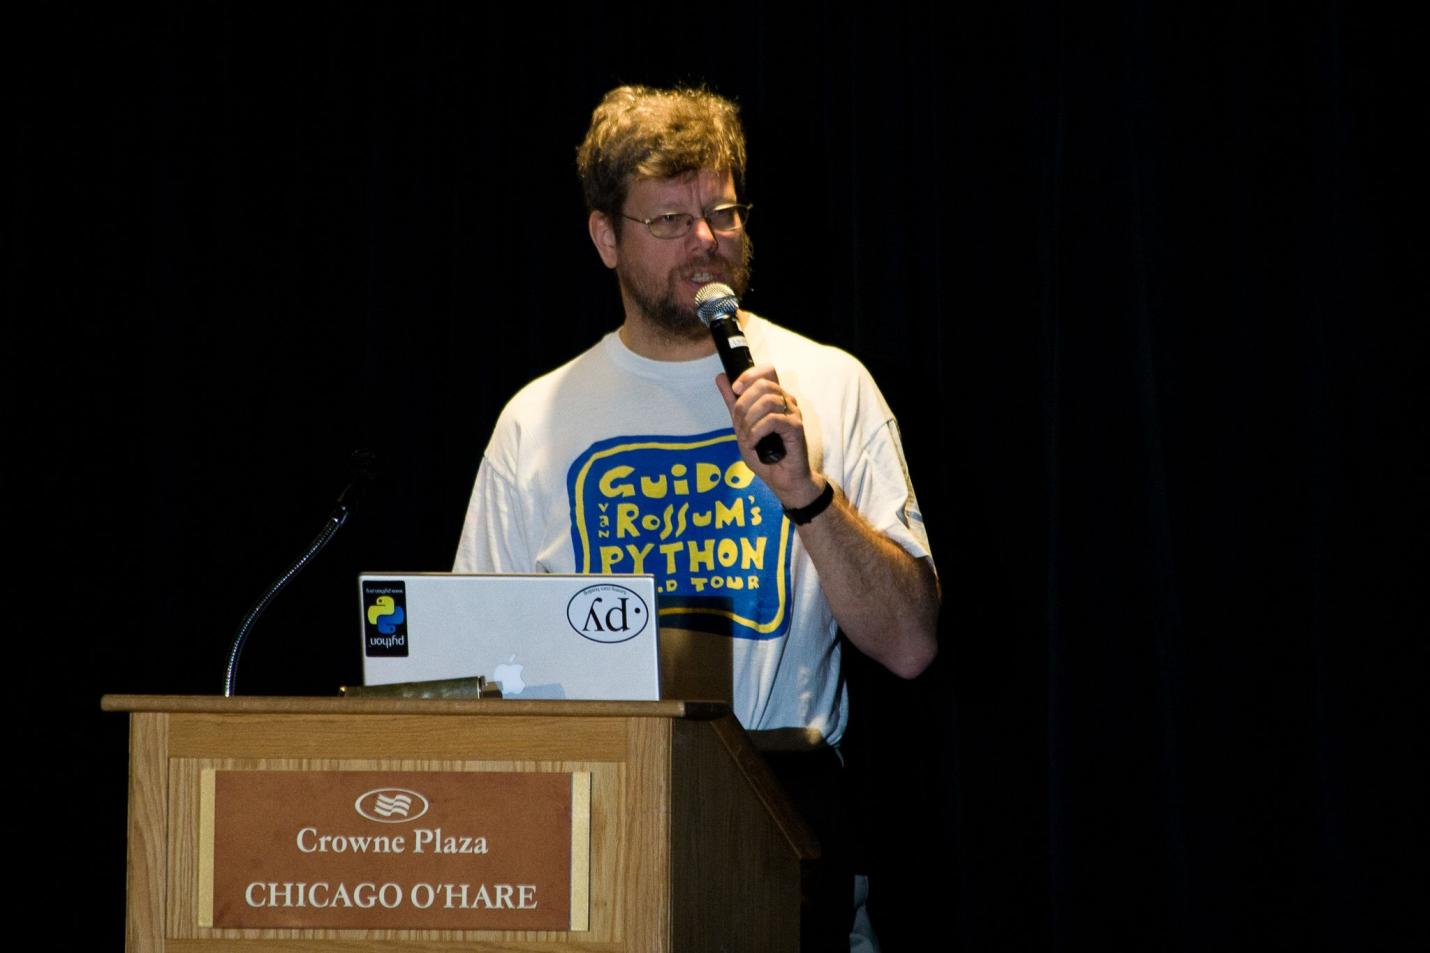
\includegraphics[width=0.6\textwidth]{images/Guido van Rossum.jpg}
    \caption{Guido van Rossum - Tác giả sáng lập Python. (Nguồn: Sauria Associates, LLC / FlickrVision)}
\end{figure}

\section{Tên gọi Python}

Tên gọi "Python" không xuất phát từ loài trăn, mà lấy cảm hứng từ chương trình hài kịch yêu thích của ông trên đài BBC: "Monty Python's Flying Circus".

\section{Hướng dẫn cài đặt Python và Anaconda}

\subsection{Cài đặt Python}
\begin{enumerate}
    \item Truy cập trang chủ Python: \url{https://www.python.org/downloads/}
    \item Tải phiên bản cài đặt (Ví dụ: Python 3.14.7 cho Windows).
    \item Mở file cài đặt. \textbf{Lưu ý quan trọng:} Nhớ tick vào ô "Add python.exe to PATH" trước khi bấm "Install Now".
    \item Bấm "Close" khi cài đặt thành công. Có thể chọn "Disable path length limit" nếu cần.
\end{enumerate}

\begin{figure}[h]
    \centering
    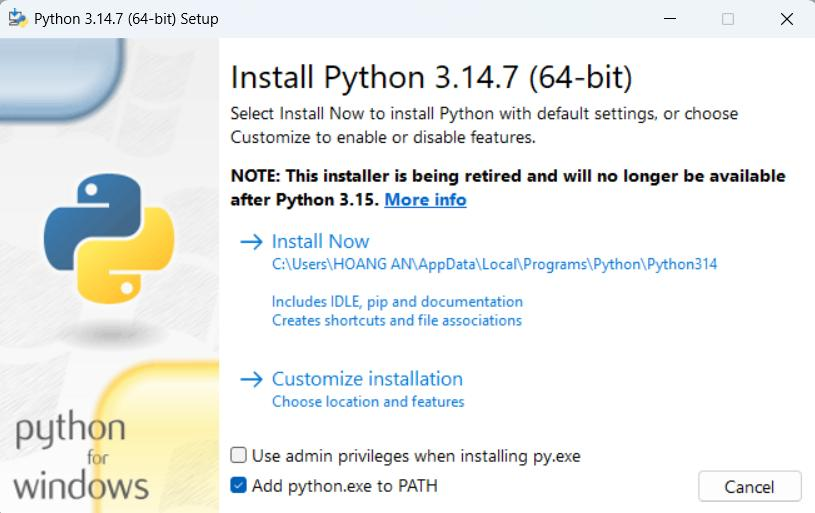
\includegraphics[width=0.6\textwidth]{images/B2.jpg}
    \caption{Tick chọn Add python.exe to PATH trong quá trình cài đặt}
\end{figure}

\subsection{Cài đặt Anaconda/Miniconda}
Anaconda là một nền tảng phân phối Python và R phục vụ cho khoa học dữ liệu.

\begin{enumerate}
    \item Truy cập trang tải Anaconda: \url{https://www.anaconda.com/download}
    \item Tải bản cài đặt Anaconda Distribution hoặc Miniconda.
    \item Mở file cài đặt, chọn "Just Me", chọn đường dẫn lưu (ví dụ: \texttt{C:\textbackslash miniconda3}).
    \item Trong phần Advanced Installation Options, có thể tick chọn "Register Miniconda3 as my default Python".
    \item Nhấn "Install" và đợi quá trình cài đặt hoàn tất.
\end{enumerate}

\subsection{Tạo môi trường Conda}
Sau khi cài đặt Anaconda/Miniconda, mở Anaconda Prompt và sử dụng lệnh sau để tạo một môi trường ảo (ví dụ tên là \texttt{ai}) với phiên bản Python 3.14:
\begin{lstlisting}[language=bash]
conda create -n ai python=3.14 anaconda
\end{lstlisting}
Xác nhận tiến trình cài đặt các gói bằng cách gõ \texttt{y} (yes) khi được yêu cầu. Sau đó kích hoạt môi trường bằng lệnh \texttt{conda activate ai}. Mọi thư viện cài thêm từ lúc này chỉ thuộc về môi trường \texttt{ai}, nhờ vậy các dự án khác nhau không xung đột phiên bản thư viện với nhau.

\subsection{Làm việc với Jupyter Notebook}
\label{sec:jupyter}

Các ví dụ và bài thực hành của giáo trình được viết dưới dạng \textbf{notebook} (tệp \texttt{.ipynb}): một tài liệu tương tác gồm nhiều \textbf{ô} (cell), trong đó ô mã chứa lệnh Python, còn ô văn bản (Markdown) chứa phần giải thích. Jupyter bắt nguồn từ dự án IPython do Fernando Pérez khởi xướng năm 2001 và trở thành Project Jupyter năm 2014 (Kluyver và cộng sự, 2016). Notebook cho phép chạy từng đoạn mã và xem ngay kết quả, kể cả biểu đồ, ở bên dưới. Vì vậy notebook rất phù hợp để khám phá dữ liệu và thử nghiệm mô hình.

\begin{lstlisting}[language=bash, caption={Mở JupyterLab trong môi trường ai}]
conda activate ai
jupyter lab
\end{lstlisting}

Lệnh \texttt{jupyter lab} mở giao diện JupyterLab trên trình duyệt. Một số điểm cần nắm:
\begin{itemize}
    \item Tổ hợp phím \texttt{Shift + Enter} chạy ô hiện tại và chuyển xuống ô kế tiếp.
    \item Biến tạo ở một ô được giữ trong bộ nhớ của \textbf{kernel} và dùng được ở các ô sau, nên thứ tự chạy các ô quyết định kết quả. Trước khi nộp bài, hãy chọn \textit{Restart Kernel and Run All Cells} để chắc chắn notebook chạy đúng từ đầu đến cuối.
    \item Visual Studio Code và Google Colab cũng mở được tệp \texttt{.ipynb} với cách dùng tương tự.
\end{itemize}

\section{Tóm tắt chương}

Trong chương này, chúng ta đã tìm hiểu:
\begin{itemize}
    \item Khái niệm cơ bản về Python và ứng dụng của nó.
    \item Lịch sử hình thành chi tiết qua từng giai đoạn (từ Python 0.9.0 đến Python 3.x).
    \item Tiểu sử của tác giả Guido van Rossum và nguồn gốc tên gọi thú vị của Python.
    \item Các bước cài đặt môi trường lập trình cơ bản với Python và Anaconda.
    \item Cách tạo, kích hoạt môi trường Conda và làm việc với Jupyter Notebook.
\end{itemize}

\section{Bài tập}
\begin{enumerate}
    \item Cài đặt Anaconda hoặc Miniconda, tạo và kích hoạt môi trường \texttt{ai}, rồi kiểm tra phiên bản Python bằng lệnh \texttt{python --version}.
    \item Mở JupyterLab và tạo một notebook gồm một ô Markdown giới thiệu bản thân và một ô mã in ra lời chào. Lưu thành tệp \texttt{.ipynb}, khởi động lại kernel rồi chạy lại toàn bộ notebook.
    \item Trong notebook, chạy lệnh \texttt{import this} để đọc ``The Zen of Python''. Chọn hai nguyên tắc và giải thích ý nghĩa của chúng bằng ví dụ cụ thể.
\end{enumerate}

% ---------------------------------------------------------
\section*{Tài liệu tham khảo của chương}
\addcontentsline{toc}{section}{Tài liệu tham khảo của chương}
% ---------------------------------------------------------
\begin{enumerate}
    \item Kluyver, T. et al. (2016). Jupyter Notebooks -- a publishing format for reproducible computational workflows. In \textit{Positioning and Power in Academic Publishing}, 87--90. IOS Press.
    \item Python Software Foundation. \textit{The Python Tutorial}. \url{https://docs.python.org/3/tutorial/}
\end{enumerate}        % Chương 1
\chapter{Cú pháp Python cơ bản}
\label{chap:python-basics}

Chương này trình bày các khái niệm nền tảng trong lập trình Python: biến, kiểu dữ liệu, toán tử, cấu trúc dữ liệu, cấu trúc điều khiển, vòng lặp và hàm. Đây là các kiến thức bắt buộc trước khi đi vào xử lý dữ liệu và Machine Learning, vì mọi đoạn mã ở các chương sau đều được ghép từ những thành phần này. Các ví dụ được chọn có chủ đích: mỗi ví dụ là hình thức sơ khai của một thao tác sẽ gặp lại trong học máy, như tính độ chính xác, lưu siêu tham số hay lặp Gradient Descent.

\noindent Sau khi học xong chương này, người học có khả năng:
\begin{itemize}
    \item Khai báo biến, nhận biết và chuyển đổi các kiểu dữ liệu cơ bản; định dạng chuỗi bằng f-string.
    \item Sử dụng các toán tử số học, toán tử gán, toán tử so sánh và toán tử logic.
    \item Lựa chọn đúng cấu trúc dữ liệu: list, tuple, dictionary và set.
    \item Viết cấu trúc rẽ nhánh \texttt{if-elif-else}, vòng lặp \texttt{for}, \texttt{while} và list comprehension.
    \item Định nghĩa hàm có tham số mặc định, trả về nhiều giá trị; sử dụng hàm \texttt{lambda}.
    \item Nạp thư viện bằng \texttt{import} và nhận biết các tên viết tắt quy ước \texttt{np}, \texttt{pd}, \texttt{plt}.
\end{itemize}

\section{Biến và Kiểu dữ liệu}

Trong Python, biến được khởi tạo tự động khi gán giá trị. Python là ngôn ngữ \textit{dynamically typed} (định kiểu động): kiểu của biến được xác định từ giá trị gán cho nó, không cần khai báo trước.

\begin{definition}[Biến trong Python]
Biến là tên gọi đại diện cho một vùng nhớ chứa dữ liệu. Giá trị của biến có thể thay đổi trong quá trình thực thi chương trình.
\end{definition}

\subsection{Các kiểu dữ liệu cơ bản}
Dựa trên nền tảng Python Basic, dưới đây là bảng tổng hợp các kiểu dữ liệu cốt lõi thường xuyên được sử dụng:

\begin{table}[H]
\centering
\begin{tabular}{|l|l|l|}
\hline
\textbf{Tên} & \textbf{Kiểu dữ liệu} & \textbf{Ví dụ} \\
\hline
\texttt{str} & Kiểu chuỗi (string) & \texttt{a = 'Thien Thanh'} \\
\hline
\texttt{int} & Kiểu số nguyên & \texttt{a = 79} \\
\hline
\texttt{float} & Kiểu số thực & \texttt{a = 7.6} \\
\hline
\texttt{NoneType} & Kiểu None & \texttt{a = None} \\
\hline
\texttt{bool} & Kiểu luận lý (True, False) & \texttt{a = True} \\
\hline
\texttt{list} & Kiểu danh sách & \texttt{a = [3, 2, 1, 5]} \\
\hline
\texttt{tuple} & Kiểu bộ & \texttt{a = (1, 5, 3)} \\
\hline
\texttt{dict} & Kiểu từ điển & \texttt{b = \{'one': 1, 'four': 4\}} \\
\hline
\texttt{set} & Kiểu tập hợp & \texttt{a = \{1, 3, 5\}} \\
\hline
\end{tabular}
\caption{Các kiểu dữ liệu cơ bản trong Python}
\label{tab:python-types}
\end{table}

Để kiểm tra kiểu dữ liệu của một biến trong Python, ta sử dụng hàm \texttt{type()}. Mọi nội dung đứng sau dấu \texttt{\#} trên một dòng là \textbf{chú thích}, Python bỏ qua khi chạy:

\begin{lstlisting}[caption={Kiểm tra kiểu dữ liệu}]
a = 7
print(type(a))  # Output: <class 'int'>
\end{lstlisting}

\subsection{Chuyển đổi kiểu và định dạng chuỗi}

Các hàm \texttt{int()}, \texttt{float()}, \texttt{str()}, \texttt{bool()} chuyển một giá trị sang kiểu tương ứng. Thao tác này rất thường gặp: dữ liệu đọc từ tệp văn bản luôn ở dạng chuỗi, phải chuyển sang số trước khi tính toán. Để in kết quả, cách gọn nhất là \textbf{f-string}: chuỗi có tiền tố \texttt{f}, trong đó mỗi biểu thức đặt trong cặp ngoặc nhọn được thay bằng giá trị của nó. Phần sau dấu hai chấm quy định cách hiển thị: \texttt{:.3f} là số thực với 3 chữ số thập phân, \texttt{:.2\%} là phần trăm với 2 chữ số thập phân.

\begin{lstlisting}[caption={Chuyển đổi kiểu và f-string}]
s = "3.75"              # du lieu doc tu tep o dang chuoi
x = float(s)            # chuyen sang so thuc
n = int(x)              # cat bo phan thap phan
print(x + 1, n)         # 4.75 3

name = "KNN"
acc = 0.91234
print(f"Mo hinh {name}: do chinh xac = {acc:.2%}")
# Mo hinh KNN: do chinh xac = 91.23%
print(f"MSE = {0.123456:.3f}")      # MSE = 0.123
\end{lstlisting}

\section{Toán tử trong Python}

Toán tử là thành phần không thể thiếu để thực hiện các phép tính từ cơ bản đến phức tạp trong các thuật toán.

\subsection{Toán tử cơ bản}
\begin{table}[H]
\centering
\begin{tabular}{|l|c|l|l|}
\hline
\textbf{Tên toán tử} & \textbf{Ký hiệu} & \textbf{Ví dụ} & \textbf{Kết quả} \\
\hline
Cộng & \texttt{+} & \texttt{3 + 7} & \texttt{10} \\
\hline
Trừ & \texttt{-} & \texttt{7 - 2} & \texttt{5} \\
\hline
Nhân & \texttt{*} & \texttt{2 * 7} & \texttt{14} \\
\hline
Chia & \texttt{/} & \texttt{7 / 5} & \texttt{1.4} \\
\hline
Chia lấy phần nguyên & \texttt{//} & \texttt{10 // 4} & \texttt{2} \\
\hline
Chia lấy phần dư & \texttt{\%} & \texttt{9 \% 5} & \texttt{4} \\
\hline
Lấy mũ & \texttt{**} & \texttt{2 ** 3} & \texttt{8} \\
\hline
\end{tabular}
\caption{Các toán tử số học cơ bản}
\end{table}

\subsection{Toán tử gán mở rộng}
Để mã nguồn ngắn gọn hơn, Python hỗ trợ các toán tử gán mở rộng kết hợp phép tính và phép gán: \texttt{a += 3} tương đương \texttt{a = a + 3}.
\begin{table}[H]
\centering
\begin{tabular}{|l|c|l|l|}
\hline
\textbf{Tên toán tử} & \textbf{Ký hiệu} & \textbf{Ví dụ} & \textbf{Kết quả} \\
\hline
Cộng & \texttt{+=} & \texttt{a = 7; a += 3} & \texttt{10} \\
\hline
Trừ & \texttt{-=} & \texttt{b = 9; b -= 4} & \texttt{5} \\
\hline
Nhân & \texttt{*=} & \texttt{a = 2; a *= 7} & \texttt{14} \\
\hline
Chia & \texttt{/=} & \texttt{a = 7; a /= 5} & \texttt{1.4} \\
\hline
Chia lấy phần nguyên & \texttt{//=} & \texttt{a = 10; a //= 4} & \texttt{2} \\
\hline
Chia lấy phần dư & \texttt{\%=} & \texttt{a = 9; a \%= 5} & \texttt{4} \\
\hline
Lấy mũ & \texttt{**=} & \texttt{a = 2; a **= 3} & \texttt{8} \\
\hline
\end{tabular}
\caption{Các toán tử gán mở rộng}
\end{table}

\subsection{Toán tử so sánh và toán tử logic}

Toán tử so sánh trả về giá trị kiểu \texttt{bool}. Cần phân biệt dấu \texttt{=} (phép gán) với \texttt{==} (phép so sánh bằng). Toán tử logic \texttt{and}, \texttt{or}, \texttt{not} kết hợp nhiều điều kiện. Đây là nền tảng của cấu trúc rẽ nhánh ở Mục~\ref{sec:control-flow} và của phép lọc dữ liệu theo điều kiện ở Chương~\ref{chap:numpy-pandas}.

\begin{table}[H]
\centering
\begin{tabular}{|l|c|l|l|}
\hline
\textbf{Ý nghĩa} & \textbf{Ký hiệu} & \textbf{Ví dụ} & \textbf{Kết quả} \\
\hline
Bằng & \texttt{==} & \texttt{3 == 3.0} & \texttt{True} \\
\hline
Khác & \texttt{!=} & \texttt{2 != 3} & \texttt{True} \\
\hline
Lớn hơn, nhỏ hơn & \texttt{>}, \texttt{<} & \texttt{5 > 7} & \texttt{False} \\
\hline
Lớn hơn hoặc bằng, nhỏ hơn hoặc bằng & \texttt{>=}, \texttt{<=} & \texttt{4 <= 4} & \texttt{True} \\
\hline
Và (đúng khi cả hai đúng) & \texttt{and} & \texttt{True and False} & \texttt{False} \\
\hline
Hoặc (đúng khi ít nhất một vế đúng) & \texttt{or} & \texttt{True or False} & \texttt{True} \\
\hline
Phủ định & \texttt{not} & \texttt{not True} & \texttt{False} \\
\hline
Thuộc về & \texttt{in} & \texttt{2 in [1, 2, 3]} & \texttt{True} \\
\hline
\end{tabular}
\caption{Các toán tử so sánh và toán tử logic}
\end{table}

\begin{lstlisting}[caption={Kết hợp điều kiện bằng toán tử logic}]
acc, f1 = 0.92, 0.78
print(acc > 0.9 and f1 > 0.8)       # False
print(acc > 0.9 or f1 > 0.8)        # True
print(not acc > 0.9)                # False
print("svm" in ["knn", "svm"])      # True
\end{lstlisting}

\section{Hàm toán học trong Python}

Đối với các ứng dụng khoa học dữ liệu, thư viện \texttt{math} cung cấp các hằng số và hàm tính toán nâng cao. Để sử dụng, ta cần import thư viện (cơ chế \texttt{import} được trình bày ở Mục~\ref{sec:python-import}):

\begin{lstlisting}[caption={Import thư viện math}]
import math
\end{lstlisting}

\subsection{Các hằng số toán học}
\begin{itemize}
    \item Số Euler $e$ (cơ số của logarit tự nhiên): \texttt{math.e} $\approx 2{,}718$.
    \item Số $\pi$: \texttt{math.pi} $\approx 3{,}14159$.
\end{itemize}

\subsection{Các hàm toán học thường dùng}
\begin{table}[H]
\centering
\begin{tabular}{|c|l|l|}
\hline
\textbf{Hàm (Toán học)} & \textbf{Mã lệnh Python} & \textbf{Ví dụ} \\
\hline
$\ln x$ & \texttt{math.log(x)} & \texttt{math.log(math.e)} cho \texttt{1.0} \\
\hline
$\log_2 x$ & \texttt{math.log2(x)} & \texttt{math.log2(8)} cho \texttt{3.0} \\
\hline
$\log_{10} x$ & \texttt{math.log10(x)} & \texttt{math.log10(1000)} cho \texttt{3.0} \\
\hline
$e^x$ & \texttt{math.exp(x)} & \texttt{math.exp(0)} cho \texttt{1.0} \\
\hline
$\sqrt{x}$ & \texttt{math.sqrt(x)} & \texttt{math.sqrt(16)} cho \texttt{4.0} \\
\hline
$a^x$ & \texttt{math.pow(a, x)} & \texttt{math.pow(2, 3)} cho \texttt{8.0} \\
\hline
\end{tabular}
\caption{Một số hàm toán học từ thư viện math}
\end{table}

Các hàm của \texttt{math} chỉ nhận \textbf{một số}. Để áp dụng một hàm lên cả mảng hàng nghìn số, ta dùng các hàm cùng tên của NumPy như \texttt{np.log}, \texttt{np.exp} (Chương~\ref{chap:numpy-pandas}).

\section{Cấu trúc dữ liệu nâng cao}

Đối với Machine Learning, ngoài các kiểu số và chuỗi, ta thường sử dụng bốn cấu trúc dữ liệu có sẵn của Python: List, Tuple, Dictionary và Set. Bảng~\ref{tab:python-collections} ở cuối mục so sánh bốn cấu trúc này.

\subsection{List (Danh sách)}
List là tập hợp các phần tử có thứ tự và có thể thay đổi (mutable).

\begin{lstlisting}[caption={Thao tác cơ bản trên List}]
# Khoi tao list
features = [1.2, 3.4, 5.1, 2.8]

# Truy cap va thay doi phan tu
features[0] = 0.9
features.append(4.5)

print("List sau khi cap nhat:", features)
\end{lstlisting}

Chỉ số (index) của list bắt đầu từ 0; chỉ số âm đếm từ cuối. Cú pháp \textbf{cắt lát} (slicing) \texttt{a[i:j]} lấy các phần tử từ vị trí \texttt{i} đến \textbf{trước} vị trí \texttt{j}. Quy tắc này được giữ nguyên cho mảng NumPy và bảng Pandas ở Chương~\ref{chap:numpy-pandas}.

\begin{lstlisting}[caption={Chỉ số, cắt lát và các hàm dựng sẵn trên List}]
scores = [7, 9, 4, 10, 6]
print(scores[0], scores[-1])                     # 7 6
print(scores[1:4])                               # [9, 4, 10]
print(len(scores), sum(scores), max(scores))     # 5 36 10
print(sorted(scores))                            # [4, 6, 7, 9, 10]
\end{lstlisting}

\subsection{Tuple (Bộ)}
Tuple giống list nhưng \textbf{không thể thay đổi} (immutable) sau khi tạo. Tuple thường dùng để biểu diễn những giá trị đi cùng nhau và không được sửa, ví dụ kích thước của một bảng dữ liệu: thuộc tính \texttt{shape} của mảng NumPy chính là một tuple $(n, d)$. Thao tác \textbf{tách tuple} (unpacking) gán từng phần tử cho từng biến.

\begin{lstlisting}[caption={Tuple và phép tách tuple}]
shape = (150, 4)        # (so mau, so dac trung) cua bo du lieu Iris
n, d = shape            # tach tuple
print(n, d)             # 150 4
# shape[0] = 200        # loi TypeError: tuple khong the thay doi
\end{lstlisting}

\subsection{Dictionary (Từ điển)}
Dictionary lưu các cặp \textbf{khóa -- giá trị} (key -- value) và truy xuất giá trị theo khóa thay vì theo vị trí. Trong học máy, dictionary được dùng để lưu bộ siêu tham số của mô hình, lưu lưới siêu tham số cần thử (Chương~\ref{chap:validation}) hay lưu bảng ánh xạ nhãn chữ sang số (Chương~\ref{chap:preprocessing}).

\begin{lstlisting}[caption={Thao tác trên Dictionary}]
params = {"n_neighbors": 5, "weights": "uniform"}
params["n_neighbors"] = 7           # sua gia tri theo khoa
params["metric"] = "euclidean"      # them cap khoa - gia tri moi
print(params["n_neighbors"])        # 7
print(list(params.keys()))          # ['n_neighbors', 'weights', 'metric']
for key, value in params.items():   # duyet tung cap khoa - gia tri
    print(key, "=", value)
\end{lstlisting}

\subsection{Set (Tập hợp)}
Set là tập hợp các phần tử \textbf{không trùng lặp} và không có thứ tự. Set thường dùng để tìm các giá trị khác nhau, ví dụ các lớp xuất hiện trong vector nhãn, hoặc để tính giao, hợp giữa hai tập.

\begin{lstlisting}[caption={Tìm các giá trị khác nhau bằng Set}]
labels = ["spam", "ham", "spam", "ham", "spam"]
classes = set(labels)
print(len(classes), sorted(classes))    # 2 ['ham', 'spam']
print({1, 2, 3} & {2, 3, 4})            # {2, 3}   (phep giao)
\end{lstlisting}

\begin{table}[H]
\centering
\begin{tabular}{|l|c|c|c|p{5.1cm}|}
\hline
\textbf{Cấu trúc} & \textbf{Ký hiệu} & \textbf{Có thứ tự} & \textbf{Sửa được} & \textbf{Dùng trong học máy} \\
\hline
List & \texttt{[ ]} & Có & Có & Danh sách đặc trưng, lịch sử mất mát theo epoch \\
\hline
Tuple & \texttt{( )} & Có & Không & Kích thước mảng $(n, d)$, trả về nhiều giá trị \\
\hline
Dictionary & \texttt{\{k: v\}} & Có\footnotemark & Có & Siêu tham số, ánh xạ nhãn \\
\hline
Set & \texttt{\{ \}} & Không & Có & Tập các lớp, tập từ vựng \\
\hline
\end{tabular}
\caption{So sánh bốn cấu trúc dữ liệu có sẵn của Python}
\label{tab:python-collections}
\end{table}
\footnotetext{Từ Python 3.7, dictionary giữ đúng thứ tự thêm vào của các khóa. Khóa không được trùng nhau.}

\section{Cấu trúc điều khiển và Vòng lặp}
\label{sec:control-flow}

Python dùng \textbf{thụt lề} (thường là 4 dấu cách) để xác định khối lệnh thuộc về một câu lệnh điều kiện, vòng lặp hay hàm, thay cho cặp ngoặc nhọn của C hay Java. Thụt lề sai sẽ gây lỗi \texttt{IndentationError} hoặc làm chương trình chạy sai logic.

\subsection{Câu lệnh điều kiện if-else}
\begin{lstlisting}[caption={Sử dụng cấu trúc điều kiện}]
score = 0.85

if score >= 0.8:
    print("Mo hinh dat do chinh xac cao")
else:
    print("Can can thiep hoac toi uu them")
\end{lstlisting}

Khi có nhiều hơn hai trường hợp, dùng thêm \texttt{elif}. Python kiểm tra lần lượt từ trên xuống và chỉ thực hiện khối lệnh của \textbf{điều kiện đúng đầu tiên}.

\begin{lstlisting}[caption={Nhiều nhánh với if-elif-else}]
bmi = 23.5
if bmi < 18.5:
    group = "thieu can"
elif bmi < 25:
    group = "binh thuong"
elif bmi < 30:
    group = "thua can"
else:
    group = "beo phi"
print(group)        # binh thuong
\end{lstlisting}

Một chuỗi \texttt{if-elif} lồng nhau trên các đặc trưng chính là cách một \textbf{cây quyết định} đưa ra dự đoán. Khác biệt duy nhất là cây quyết định tự học các ngưỡng như 18,5 hay 25 từ dữ liệu (Chương~\ref{chap:classify}).

\subsection{Vòng lặp for}
Vòng lặp \texttt{for} duyệt lần lượt từng phần tử của một dãy. Ba hàm thường đi kèm là: \texttt{range(n)} sinh dãy số $0, 1, \dots, n-1$; \texttt{zip(a, b)} duyệt song song hai dãy; \texttt{enumerate(a)} trả về đồng thời chỉ số và giá trị.

\begin{lstlisting}[caption={Vòng lặp for với zip, range và enumerate}]
y_true = [1, 0, 1, 1, 0]
y_pred = [1, 0, 0, 1, 1]

correct = 0
for t, p in zip(y_true, y_pred):    # duyet song song hai list
    if t == p:
        correct += 1
print("Do chinh xac:", correct / len(y_true))     # Do chinh xac: 0.6

for epoch in range(3):              # epoch = 0, 1, 2
    print("Epoch", epoch)

for i, model in enumerate(["knn", "svm"]):  # chi so va gia tri
    print(i, model)                 # 0 knn, roi 1 svm
\end{lstlisting}

\noindent Đoạn mã đầu tiên tính \textbf{độ chính xác} (accuracy) của một bộ phân lớp: tỉ lệ mẫu có nhãn dự đoán trùng nhãn thật, ở đây là $3/5 = 0{,}6$. Độ đo này được dùng xuyên suốt Chương~\ref{chap:classify} và được phân tích kỹ ở Chương~\ref{chap:validation}.

\subsection{Vòng lặp while, break và continue}
Vòng lặp \texttt{while} lặp lại \textbf{chừng nào điều kiện còn đúng}. Nó phù hợp khi chưa biết trước số lần lặp, ví dụ lặp một thuật toán tối ưu cho đến khi hội tụ. Đoạn mã dưới đây tìm điểm cực tiểu của hàm $f(w) = (w - 3)^2$: mỗi bước dịch $w$ ngược chiều đạo hàm $f'(w) = 2(w - 3)$ một lượng tỉ lệ với hệ số $0{,}1$, và dừng khi bước dịch đủ nhỏ. Đây chính là thuật toán \textbf{Gradient Descent}, sẽ được trình bày đầy đủ ở Chương~\ref{chap:regression}.

\begin{lstlisting}[caption={Vòng lặp while: lặp đến khi hội tụ}]
w, lr = 0.0, 0.1        # diem xuat phat va he so buoc
step = 1.0
n_iter = 0
while abs(step) > 1e-4:
    grad = 2 * (w - 3)  # dao ham cua f(w) = (w - 3)^2
    step = lr * grad
    w = w - step
    n_iter += 1
print(n_iter, round(w, 4))      # 40 2.9996
\end{lstlisting}

\noindent Lệnh \texttt{break} thoát khỏi vòng lặp ngay lập tức; lệnh \texttt{continue} bỏ qua phần còn lại của lượt hiện tại để sang lượt kế tiếp:

\begin{lstlisting}[caption={Điều khiển vòng lặp bằng break và continue}]
for k in [1, 3, 5, 7, 9]:
    if k == 7:
        break           # thoat vong lap
    if k == 3:
        continue        # bo qua k = 3
    print(k)            # in ra 1 roi 5
\end{lstlisting}

\subsection{List comprehension}
List comprehension tạo một list mới từ một dãy trong \textbf{một dòng lệnh}, có thể kèm điều kiện lọc. Cú pháp tổng quát: \texttt{[biểu thức for phần\_tử in dãy if điều\_kiện]}.

\begin{lstlisting}[caption={List comprehension}]
x = [1, 2, 3, 4]
print([v ** 2 for v in x])                  # [1, 4, 9, 16]
print([v for v in x if v % 2 == 0])         # [2, 4]
errors = [(t - p) ** 2 for t, p in zip([3, 5], [2.5, 6])]
print(errors)                               # [0.25, 1]
\end{lstlisting}

\noindent Vòng lặp của Python dễ viết nhưng chậm khi dữ liệu lớn. Ở Chương~\ref{chap:numpy-pandas}, phần lớn các vòng lặp trên sẽ được thay bằng phép toán \textbf{vector hóa} của NumPy, nhanh hơn hàng chục đến hàng trăm lần.

\section{Hàm}
\label{sec:python-functions}

Hàm (function) đóng gói một đoạn mã thành một khối có tên để dùng lại nhiều lần. Hàm được định nghĩa bằng từ khóa \texttt{def}, nhận các \textbf{tham số} và trả kết quả về bằng \texttt{return}. Chuỗi đặt ngay dưới dòng \texttt{def} là \textbf{docstring}, mô tả công dụng của hàm.

\subsection{Định nghĩa hàm}
Hàm dưới đây tính \textbf{sai số bình phương trung bình} (MSE), độ đo cơ bản của bài toán hồi quy ở Chương~\ref{chap:regression}:
\begin{equation*}
    \mathrm{MSE} = \frac{1}{n}\sum_{i=1}^{n}\big(y_i - \hat{y}_i\big)^2 .
\end{equation*}

\begin{lstlisting}[caption={Định nghĩa hàm tính MSE}]
def mse(y_true, y_pred):
    """Tinh sai so binh phuong trung binh."""
    total = 0
    for t, p in zip(y_true, y_pred):
        total += (t - p) ** 2
    return total / len(y_true)

print(mse([3, 5, 2], [2.5, 6, 2]))      # 0.4166666666666667
\end{lstlisting}

\noindent Kiểm tra bằng tay: $\big[(3 - 2{,}5)^2 + (5 - 6)^2 + (2 - 2)^2\big] / 3 = (0{,}25 + 1 + 0)/3 \approx 0{,}4167$.

\subsection{Tham số mặc định và tham số từ khóa}
Tham số có thể được gán \textbf{giá trị mặc định}, khi đó người gọi hàm có thể bỏ qua nó. Khi gọi hàm, có thể truyền tham số theo \textbf{tên} (tham số từ khóa) thay vì theo vị trí. Mọi mô hình của scikit-learn đều nhận siêu tham số theo cách này, ví dụ \texttt{KNeighborsClassifier(n\_neighbors=5)}.

\begin{lstlisting}[caption={Tham số mặc định và tham số từ khóa}]
def scale(x, factor=1.0, shift=0.0):
    return x * factor + shift

print(scale(10))            # 10.0   (dung gia tri mac dinh)
print(scale(10, 0.5))       # 5.0    (truyen theo vi tri)
print(scale(10, shift=-3))  # 7.0    (truyen theo ten)
\end{lstlisting}

\subsection{Trả về nhiều giá trị}
Khi \texttt{return} nhiều giá trị cách nhau bởi dấu phẩy, Python đóng gói chúng thành một tuple. Bên gọi hàm dùng phép tách tuple để nhận từng giá trị. Hàm \texttt{train\_test\_split} của scikit-learn trả về bốn giá trị theo đúng cách này.

\begin{lstlisting}[caption={Hàm trả về nhiều giá trị}]
def min_max(values):
    return min(values), max(values)

lo, hi = min_max([4, 8, 1, 6])
print(lo, hi)               # 1 8
\end{lstlisting}

\subsection{Hàm lambda}
Hàm \texttt{lambda} là hàm ẩn danh viết trên một dòng, thường dùng làm tham số cho một hàm khác. Ví dụ, khóa sắp xếp của \texttt{sorted}, hay hàm áp dụng lên từng phần tử của một cột dữ liệu bằng phương thức \texttt{apply} của Pandas (Chương~\ref{chap:numpy-pandas}).

\begin{lstlisting}[caption={Hàm lambda làm khóa sắp xếp}]
square = lambda v: v ** 2
print(square(4))                                    # 16
results = [("knn", 0.91), ("svm", 0.95), ("tree", 0.88)]
best = sorted(results, key=lambda r: r[1], reverse=True)[0]
print(best)                                         # ('svm', 0.95)
\end{lstlisting}

\section{Module và thư viện}
\label{sec:python-import}

Một \textbf{module} là một tệp mã Python chứa các hàm, lớp và hằng số. Một \textbf{thư viện} (package) gồm nhiều module. Lệnh \texttt{import} nạp module vào chương trình theo ba cách:

\begin{lstlisting}[caption={Ba cách import}]
import math                     # nap ca module, goi qua ten module
from math import sqrt, pi       # chi nap mot so ten
import numpy as np              # dat ten viet tat theo quy uoc

print(math.floor(2.7), sqrt(16), round(pi, 2))   # 2 4.0 3.14
print(np.mean([1, 2, 3, 4]))                     # 2.5
\end{lstlisting}

Cộng đồng Python thống nhất một số tên viết tắt mà mọi tài liệu đều dùng. Giáo trình này tuân theo các quy ước đó:

\begin{table}[H]
\centering
\begin{tabular}{|p{6.4cm}|p{3.6cm}|p{3.8cm}|}
\hline
\textbf{Câu lệnh} & \textbf{Công dụng} & \textbf{Trình bày ở} \\
\hline
\texttt{import numpy as np} & Tính toán trên mảng & Chương~\ref{chap:numpy-pandas} \\
\hline
\texttt{import pandas as pd} & Bảng dữ liệu & Chương~\ref{chap:numpy-pandas} \\
\hline
\texttt{import matplotlib.pyplot as plt} & Vẽ biểu đồ & Chương~\ref{chap:numpy-pandas} \\
\hline
\texttt{from sklearn... import ...} & Các mô hình học máy & Chương~\ref{chap:preprocessing} trở đi \\
\hline
\texttt{import torch} & Tự động tính đạo hàm & Lab 8, Chương~\ref{chap:labs} \\
\hline
\end{tabular}
\caption{Tên viết tắt quy ước của các thư viện dùng trong giáo trình}
\end{table}

Các thư viện này có sẵn trong bộ cài Anaconda (Chương~\ref{chap:intro}). Nếu dùng bản Python cài riêng, có thể cài thêm bằng lệnh \texttt{pip install numpy pandas matplotlib scikit-learn} trong cửa sổ dòng lệnh.

\section{Tóm tắt chương}
Trong chương này, chúng ta đã nắm được:
\begin{itemize}
    \item Cách khai báo biến, các kiểu dữ liệu cơ bản, chuyển đổi kiểu và định dạng chuỗi bằng f-string.
    \item Các toán tử số học, toán tử gán mở rộng, toán tử so sánh và toán tử logic.
    \item Cách sử dụng thư viện \texttt{math} cho các hàm toán học trên từng số.
    \item Bốn cấu trúc dữ liệu: List (có thứ tự, sửa được), Tuple (không sửa được), Dictionary (cặp khóa -- giá trị), Set (không trùng lặp).
    \item Cấu trúc rẽ nhánh \texttt{if-elif-else}; vòng lặp \texttt{for} với \texttt{range}, \texttt{zip}, \texttt{enumerate}; vòng lặp \texttt{while} với \texttt{break}, \texttt{continue}; list comprehension.
    \item Định nghĩa hàm bằng \texttt{def}, tham số mặc định, tham số từ khóa, trả về nhiều giá trị và hàm \texttt{lambda}.
    \item Nạp thư viện bằng \texttt{import} và các tên viết tắt quy ước \texttt{np}, \texttt{pd}, \texttt{plt}.
\end{itemize}

\section{Bài tập}
\begin{enumerate}
    \item Cho list điểm \texttt{[7.5, 8, 6, 9.5, 5]}. Chỉ dùng vòng lặp \texttt{for}, không dùng thư viện, hãy tính điểm trung bình và độ lệch chuẩn $s = \sqrt{\frac{1}{n}\sum_i (x_i - \bar{x})^2}$. In kết quả với hai chữ số thập phân bằng f-string.
    \item Viết hàm \texttt{accuracy(y\_true, y\_pred)} trả về tỉ lệ dự đoán đúng. Kiểm tra với hai list ở ví dụ vòng lặp \texttt{for} (kết quả phải là $0{,}6$), rồi viết lại thân hàm bằng một dòng list comprehension.
    \item Dùng dictionary đếm số lần xuất hiện của mỗi từ trong câu \texttt{"the cat and the hat and the bat"}. Đây là ý tưởng của phương pháp Count Vectorizer ở Chương~\ref{chap:preprocessing}.
    \item Viết hàm \texttt{label\_encode(values)} gán cho mỗi giá trị khác nhau một số nguyên theo thứ tự xuất hiện. Hàm trả về hai giá trị: list mã số và dictionary ánh xạ. Ví dụ: \texttt{["red", "green", "blue", "red"]} cho \texttt{[0, 1, 2, 0]} và \texttt{\{"red": 0, "green": 1, "blue": 2\}}.
    \item Sửa vòng lặp \texttt{while} tìm cực tiểu của $f(w) = (w - 3)^2$ để thử các hệ số bước $0{,}1$; $0{,}5$; $0{,}9$ và $1{,}1$. Thêm điều kiện dừng sau tối đa 1000 bước. Đếm số bước trong từng trường hợp. Với hệ số nào $w$ không tiến về 3? Hãy giải thích bằng cách viết $w - 3$ sau mỗi bước theo $w - 3$ ở bước trước.
    \item Dùng list comprehension tạo list bình phương của các số chẵn từ 0 đến 20. Viết lại bằng vòng lặp \texttt{for} thông thường và so sánh độ dài hai cách viết.
\end{enumerate}

% ---------------------------------------------------------
\section*{Tài liệu tham khảo của chương}
\addcontentsline{toc}{section}{Tài liệu tham khảo của chương}
% ---------------------------------------------------------
\begin{enumerate}
    \item Lutz, M. (2013). \textit{Learning Python} (5th ed.). O'Reilly Media.
    \item Python Software Foundation. \textit{The Python Tutorial}. \url{https://docs.python.org/3/tutorial/}
    \item Sarkar, D., Bali, R., \& Sharma, T. (2018). \textit{Practical Machine Learning with Python}, Chương 2. Apress.
\end{enumerate}
   % Chương 2
\chapter{Lập trình hướng đối tượng trong Python}
\label{chap:oop}

Lập trình hướng đối tượng (Object-Oriented Programming - OOP) là phương pháp luận lập trình đóng vai trò then chốt trong việc thiết kế các thư viện Machine Learning hiện đại như Scikit-Learn, PyTorch và TensorFlow. Chương này trình bày các khái niệm OOP cốt lõi và hướng dẫn cách ứng dụng OOP để tự đóng gói một mô hình Machine Learning.

\section{Lớp và Đối tượng (Class and Object)}

\begin{definition}[Lớp và Đối tượng]
\textbf{Lớp (Class)} là khuôn mẫu định nghĩa các thuộc tính (dữ liệu) và phương thức (hành vi). \textbf{Đối tượng (Object)} là một thể hiện cụ thể được khởi tạo từ lớp đó.
\end{definition}

\begin{example}
Khai báo một lớp cơ bản lưu trữ mẫu dữ liệu:
\end{example}

\begin{lstlisting}[caption={Khai báo Class và tạo Object trong Python}]
class DataSample:
    def __init__(self, feature_name, value):
        self.feature_name = feature_name  # Thuoc tinh
        self.value = value

    def display_info(self):              # Phuong thuc
        print(f"Feature: {self.feature_name}, Value: {self.value}")

# Khoi tao doi tuong
sample = DataSample(feature_name="Age", value=25)
sample.display_info()
\end{lstlisting}

\section{Các phương thức đặc biệt (Magic Methods)}

Các phương thức có cú pháp hai dấu gạch dưới (\texttt{\_\_method\_\_}) giúp tùy biến hành vi của đối tượng trong Python.

\subsection{Phương thức \texttt{\_\_init\_\_} và \texttt{\_\_call\_\_}}
\begin{itemize}
    \item \texttt{\_\_init\_\_}: Hàm khởi tạo (constructor), tự động thực thi khi tạo mới một đối tượng.
    \item \texttt{\_\_call\_\_}: Cho phép gọi trực tiếp một đối tượng giống như một hàm, thường dùng khi thiết kế các Layer trong Neural Network.
\end{itemize}

\begin{lstlisting}[caption={Sử dụng phương thức \_\_call\_\_}]
class Multiplier:
    def __init__(self, factor):
        self.factor = factor

    def __call__(self, x):
        return x * self.factor

# Su dung nhu mot ham
double = Multiplier(factor=2)
print(double(5))  # Output: 10
\end{lstlisting}

\section{Tính Kế thừa (Inheritance)}

Tính kế thừa cho phép tạo một lớp mới dựa trên lớp đã có, giúp tái sử dụng mã nguồn và chuẩn hóa giao diện của các bộ biến đổi dữ liệu (Transformers).

\begin{lstlisting}[caption={Kế thừa lớp BaseTransformer trong tiền xử lý dữ liệu}, language=Python]
class BaseTransformer:
    def fit(self, arr):
        raise NotImplementedError("Phuong thuc fit() bat buoc phai duoc trien khai o lop con.")
        
    def transform(self, arr):
        raise NotImplementedError("Phuong thuc transform() bat buoc phai trien khai o lop con.")
        
    def fit_transform(self, arr):
        self.fit(arr)
        return self.transform(arr)

class MinMaxScaler(BaseTransformer):
    def fit(self, arr):
        self.min_ = min(arr)
        self.max_ = max(arr)
        return self
        
    def transform(self, arr):
        return [(x - self.min_) / (self.max_ - self.min_) for x in arr]
        
    def inverse_transform(self, arr):
        return [x * (self.max_ - self.min_) + self.min_ for x in arr]
\end{lstlisting}

\section{Quản lý thuộc tính: Siêu tham số (Hyperparameters) và Tham số học được (Learned Parameters)}

Trong thiết kế Machine Learning, ta cần phân biệt rõ giữa siêu tham số (cấu hình trước khi huấn luyện) và tham số học được (được sinh ra sau khi gọi hàm \texttt{fit}).

\begin{lstlisting}[caption={Bắt lỗi an toàn khi quản lý tham số học được}, language=Python]
class MinMaxScaler(BaseTransformer):
    def __init__(self, feature_range=(0, 1)):
        self.feature_range = feature_range  # Hyperparameter

    def fit(self, arr):
        self.min = float(min(arr))          # Learned Parameter
        self.max = float(max(arr))          # Learned Parameter
        return self

    def transform(self, arr):
        # Kiem tra an toan: Dam bao mo hinh da duoc fit()
        if not hasattr(self, 'min') or not hasattr(self, 'max'):
            raise RuntimeError("Loi: Ban phai goi ham fit() truoc khi goi transform()!")
            
        low, high = self.feature_range
        std = [(x - self.min) / (self.max - self.min) for x in arr]
        return [x * (high - low) + low for x in std]
\end{lstlisting}

\section{Thiết kế Custom Estimator chuẩn Scikit-Learn}

Trọng tâm ứng dụng OOP trong Machine Learning là đóng gói thuật toán thành một Class có các giao diện chuẩn (\texttt{fit}, \texttt{predict}, \texttt{evaluate}). Dưới đây là triển khai mô hình Hồi quy tuyến tính đơn biến (Simple Linear Regression) bằng công thức đại số.

\begin{lstlisting}[caption={Đóng gói thuật toán Simple Linear Regression}, language=Python]
class SimpleLinearRegression:
    def __init__(self):
        self.w0 = 0  
        self.w1 = 0

    def fit(self, X, y):
        n = len(X)
        mean_x = sum(X) / n
        mean_y = sum(y) / n
        
        numerator = sum((X[i] - mean_x) * (y[i] - mean_y) for i in range(n))
        denominator = sum((X[i] - mean_x) ** 2 for i in range(n))
        
        if denominator == 0:
            raise ValueError("Bao loi: Phuong sai cua X bang 0, khong the tinh toan.")

        self.w1 = numerator / denominator
        self.w0 = mean_y - (self.w1 * mean_x)
        return self

    def predict(self, X):
        return [(self.w1 * x_i + self.w0) for x_i in X]

    def evaluate(self, X, y):
        predictions = self.predict(X)
        mse = sum((predictions[i] - y[i]) ** 2 for i in range(len(y))) / len(y)
        return mse
\end{lstlisting}

\section{Mẫu thiết kế Pipeline}

Pipeline là lớp quản lý chuỗi các bước biến đổi dữ liệu nối tiếp nhau, cho phép tự động hóa toàn bộ quy trình tiền xử lý trước khi đưa vào mô hình dự đoán.

\begin{lstlisting}[caption={Triển khai cấu trúc Pipeline cơ bản}, language=Python]
class Pipeline:
    def __init__(self, steps):
        self.steps = steps

    def fit_transform(self, arr):
        data = arr
        for transformer in self.steps:
            data = transformer.fit_transform(data)
        return data

    def transform(self, arr):
        data = arr
        for transformer in self.steps:
            data = transformer.transform(data)
        return data
\end{lstlisting}

\section{Tóm tắt chương}

\begin{itemize}
    \item Khái niệm Lớp, Đối tượng và tư duy lập trình hướng đối tượng.
    \item Ứng dụng các Magic Methods (\texttt{\_\_init\_\_}, \texttt{\_\_call\_\_}) trong xây dựng Framework.
    \item Nguyên lý Kế thừa giúp tái sử dụng và quản lý mã nguồn linh hoạt.
    \item Đóng gói thuật toán Machine Learning thành Class theo giao diện tiêu chuẩn.
    \item Phân biệt rõ ràng siêu tham số và tham số học được thông qua các thuộc tính của đối tượng.
\end{itemize}

\section{Bài tập}
\begin{enumerate}
    \item Viết lớp \texttt{MeanPredictor} theo giao diện của scikit-learn: \texttt{fit(X, y)} lưu trung bình của \texttt{y} vào thuộc tính \texttt{mean\_}, còn \texttt{predict(X)} trả về một list gồm \texttt{len(X)} giá trị \texttt{mean\_}. Đây là \textbf{mô hình cơ sở} (baseline) mà mọi mô hình hồi quy ở các chương sau phải vượt qua.
    \item Viết lớp \texttt{MedianPredictor} kế thừa \texttt{MeanPredictor} và chỉ ghi đè phương thức \texttt{fit} để dùng trung vị. Giải thích vì sao không cần viết lại \texttt{predict}.
    \item Theo quy ước của scikit-learn, tên của tham số học được kết thúc bằng dấu gạch dưới (\texttt{coef\_}, \texttt{mean\_}). Sửa lớp \texttt{MinMaxScaler} ở Mục ``Quản lý thuộc tính'' theo quy ước này, đồng thời xử lý trường hợp mọi giá trị bằng nhau (\texttt{max} bằng \texttt{min}) để tránh phép chia cho 0.
    \item Trong mẫu thiết kế Pipeline, các bước biến đổi chỉ được \texttt{fit} trên dữ liệu huấn luyện rồi mới áp dụng cho dữ liệu kiểm tra. Giải thích lý do (gợi ý: hiện tượng rò rỉ dữ liệu ở Chương~\ref{chap:preprocessing}).
\end{enumerate}          % Chương 3
% =========================================================
% CHUONG: XU LY DU LIEU VOI NUMPY VA PANDAS
% =========================================================

\chapter{Xử lý và trực quan hóa dữ liệu \\ (NumPy, Pandas, Matplotlib)}
\label{chap:numpy-pandas}

Trong khoa học dữ liệu và học máy, xử lý dữ liệu đóng vai trò nền tảng. Dữ liệu thực tế thường lộn xộn, thiếu sót hoặc không đúng định dạng. Để giải quyết vấn đề này, Python cung cấp một hệ sinh thái thư viện mạnh mẽ, trong đó nổi bật nhất là NumPy và Pandas. Chương này hướng dẫn cách dùng hai thư viện để biểu diễn, truy xuất, biến đổi và tổng hợp dữ liệu --- những thao tác xuất hiện trong mọi chương sau của giáo trình. Phần cuối chương giới thiệu \textbf{Matplotlib} để trực quan hóa dữ liệu và \textbf{SciPy} cho các phép tính thống kê, tối ưu hóa. Đây là hai công cụ được dùng để vẽ hình và kiểm chứng kết quả ở các chương sau.

\noindent Sau khi học xong chương này, người học có khả năng:
\begin{itemize}
    \item Giải thích vì sao mảng NumPy nhanh hơn list của Python; phân biệt \textit{view} và \textit{copy}.
    \item Khởi tạo, cắt, lọc và biến đổi mảng; vận dụng vector hóa, broadcasting và tham số \texttt{axis}.
    \item Giải hệ phương trình tuyến tính bằng \texttt{np.linalg}.
    \item Tạo, đọc và truy xuất \texttt{DataFrame} bằng \texttt{loc}, \texttt{iloc} và điều kiện lọc.
    \item Xử lý dữ liệu thiếu, biến đổi cột, gom nhóm và gộp bảng bằng Pandas.
    \item Vẽ biểu đồ đường, phân tán, tần suất và biểu đồ hộp bằng Matplotlib theo lối hướng đối tượng; chọn đúng loại biểu đồ cho câu hỏi cần trả lời.
    \item Dùng SciPy để tính hệ số tương quan, z-score và cực tiểu hóa một hàm mất mát.
\end{itemize}

% ---------------------------------------------------------
\section{Khởi nguồn của NumPy và Pandas}
% ---------------------------------------------------------

Python vốn không được thiết kế cho tính toán số: mỗi phần tử của một list là một đối tượng riêng nằm rải rác trong bộ nhớ, và mỗi phép cộng đều phải kiểm tra kiểu dữ liệu. Các thư viện Numeric (1995) và Numarray ra đời để khắc phục điều đó. Năm 2005--2006, Travis Oliphant hợp nhất chúng thành \textbf{NumPy} (Numerical Python); bài tổng quan của Harris và cộng sự (2020) trên tạp chí \textit{Nature} ghi nhận NumPy là nền móng của toàn bộ hệ sinh thái Python khoa học, bao gồm SciPy và scikit-learn.

\textbf{Pandas} do Wes McKinney bắt đầu phát triển năm 2008 tại công ty tài chính AQR Capital, nhằm đưa vào Python kiểu làm việc với bảng dữ liệu có nhãn vốn phổ biến trong R và SQL (McKinney, 2010). Pandas được xây dựng trên NumPy: có thể hình dung mỗi cột của một bảng Pandas là một mảng có kèm nhãn.

% ---------------------------------------------------------
\section{Thư viện NumPy -- Tính toán khoa học}
% ---------------------------------------------------------

NumPy cung cấp đối tượng mảng đa chiều \texttt{ndarray}: một khối bộ nhớ liền nhau chứa các phần tử \textbf{cùng kiểu dữ liệu}. Chính hai đặc điểm này cho phép NumPy thực hiện phép tính bằng các vòng lặp đã biên dịch sẵn, nhanh hơn nhiều so với vòng lặp Python.

\subsection{Khởi tạo mảng và kiểm tra thuộc tính}

Mảng được tạo từ list của Python hoặc bằng các hàm khởi tạo những ma trận đặc biệt. Ba thuộc tính cần kiểm tra đầu tiên là \texttt{shape} (kích thước theo từng chiều), \texttt{ndim} (số chiều) và \texttt{dtype} (kiểu phần tử).

\begin{lstlisting}[caption={Khởi tạo mảng NumPy và kiểm tra thuộc tính}]
import numpy as np

arr1D = np.array([1, 2, 3, 4, 5, 6, 7, 8, 9, 10])
print("Shape 1D:", arr1D.shape, "| Dtype:", arr1D.dtype)   # (10,) | int64

arr2D = np.array([[1, 2, 3, 4],
                  [5, 6, 7, 8],
                  [9, 10, 11, 12]])
print("Shape 2D:", arr2D.shape, "| ndim:", arr2D.ndim)     # (3, 4) | 2

arr_zeros = np.zeros((3, 4))          # ma tran 3 x 4 toan so 0
arr_ones = np.ones((2, 5))            # ma tran 2 x 5 toan so 1
arr_eye = np.identity(3)              # ma tran don vi 3 x 3
arr_random = np.random.randn(3, 4)    # phan phoi chuan tac N(0, 1)
\end{lstlisting}

\noindent\textit{Lưu ý:} kiểu \texttt{int64} ở trên có thể khác trên máy khác. Với mã nguồn mới, NumPy khuyến nghị tạo số ngẫu nhiên qua \texttt{rng = np.random.default\_rng(42)} rồi gọi \texttt{rng.standard\_normal((3, 4))}, nhờ đó kết quả tái lập được.

\subsection{Thêm, xóa và sửa phần tử}

Có thể gán trực tiếp giá trị cho một phần tử. Các hàm \texttt{append}, \texttt{insert}, \texttt{delete} thì \textbf{không sửa mảng gốc} mà trả về một mảng mới. Vì kích thước của \texttt{ndarray} là cố định, mỗi lần gọi đều phải cấp phát và sao chép toàn bộ dữ liệu; do đó không nên gọi \texttt{np.append} trong vòng lặp dài, mà nên gom dữ liệu vào list rồi chuyển thành mảng một lần ở cuối.

\begin{lstlisting}[caption={Thêm, xóa và sửa phần tử mảng}]
arr1D[0] = 99                              # sua truc tiep mang goc

arr_appended = np.append(arr1D, [11, 12])  # them vao cuoi -> mang moi
arr_inserted = np.insert(arr1D, 2, 999)    # chen 999 vao vi tri 2 -> mang moi
arr_deleted = np.delete(arr1D, 0)          # xoa phan tu dau -> mang moi
arr1D[0] = 1                               # tra lai gia tri ban dau
\end{lstlisting}

\subsection{Slicing và Boolean Indexing}
\label{sec:boolean-indexing}

\textbf{Slicing} lấy một phần của mảng theo cú pháp \texttt{bắt\_đầu:kết\_thúc} trên từng chiều (không gồm vị trí kết thúc). \textbf{Boolean Indexing} dùng một mảng điều kiện đúng/sai để lọc phần tử; đây là cách lọc dữ liệu thông dụng nhất.

\begin{lstlisting}[caption={Slicing và lọc dữ liệu bằng điều kiện}]
sub_arr = arr2D[:2, :3]              # 2 dong dau, 3 cot dau
print(sub_arr)                       # [[1 2 3]
                                     #  [5 6 7]]

city_data = np.random.randn(5, 3)
pos_values = city_data[city_data > 0]    # mang 1 chieu cac gia tri duong
print("Cac gia tri > 0:", pos_values)

city_data[city_data > 0] = 0             # thay moi gia tri duong bang 0
print(city_data)
\end{lstlisting}

\paragraph{View và copy.} Đây là cái bẫy phổ biến nhất của NumPy: slicing trả về một \textbf{view}, tức một ``cửa sổ'' nhìn vào cùng vùng nhớ, chứ không sao chép dữ liệu. Sửa view đồng nghĩa với sửa mảng gốc. Muốn dữ liệu độc lập, phải gọi \texttt{.copy()}. Ngược lại, Boolean Indexing luôn trả về bản sao.

\begin{lstlisting}[caption={Slicing tạo view, không sao chép dữ liệu}]
v = arr1D[:3]
v[0] = 99
print(arr1D[:3])     # [99  2  3]  -> mang goc bi thay doi!
arr1D[0] = 1

c = arr1D[:3].copy()
c[0] = 99
print(arr1D[:3])     # [1 2 3]     -> mang goc giu nguyen
\end{lstlisting}

\subsection{Vector hóa, broadcasting và tham số axis}

\textbf{Vector hóa} (vectorization) là viết phép tính trên cả mảng thay vì lặp qua từng phần tử: mã nguồn ngắn hơn, gần với công thức toán hơn, và nhanh hơn rất nhiều. Khi thử nhân đôi một triệu số trên máy của nhóm tác giả, vòng lặp Python mất khoảng 320 ms, còn phép tính NumPy khoảng 5 ms; con số cụ thể tùy máy.

\begin{lstlisting}[caption={So sánh vòng lặp Python với vector hóa}]
x = np.arange(1_000_000, dtype=float)
y1 = [i * 2 for i in x.tolist()]     # vong lap Python: cham
y2 = x * 2                           # vector hoa: nhanh
\end{lstlisting}

\textbf{Broadcasting} là quy tắc cho phép tính toán giữa hai mảng khác kích thước: so sánh các chiều từ phải sang trái, hai chiều tương thích khi bằng nhau hoặc một trong hai bằng 1; chiều bằng 1 được ``kéo giãn'' cho khớp. Tham số \texttt{axis} chỉ chiều bị ``gộp lại'' trong phép tổng hợp: \texttt{axis=0} tính theo từng cột, \texttt{axis=1} tính theo từng dòng.

\begin{example}[Chuẩn hóa tâm bằng broadcasting]
Với \texttt{arr2D} có kích thước $(3, 4)$, trung bình theo từng cột \texttt{arr2D.mean(axis=0)} có kích thước $(4,)$ và bằng $(5, 6, 7, 8)$. Phép trừ \texttt{arr2D - arr2D.mean(axis=0)} tự động trừ vector này khỏi cả ba dòng. Đây chính là bước chuẩn hóa tâm của \texttt{StandardScaler} và PCA ở các chương sau.
\end{example}

\begin{lstlisting}[caption={Tổng hợp theo axis và broadcasting}]
print(arr2D.sum(axis=0))     # theo cot:  [15 18 21 24]
print(arr2D.sum(axis=1))     # theo dong: [10 26 42]
print(arr2D.mean())          # toan bo mang: 6.5

print(arr2D - arr2D.mean(axis=0))
# [[-4. -4. -4. -4.]
#  [ 0.  0.  0.  0.]
#  [ 4.  4.  4.  4.]]

print(arr2D.reshape(4, 3).shape, arr2D.T.shape)   # (4, 3) (4, 3)
\end{lstlisting}

\subsection{Đại số tuyến tính}

Mô-đun \texttt{np.linalg} cung cấp các phép tính đại số tuyến tính: định thức, nghịch đảo, trị riêng, SVD và giải hệ phương trình. Toán tử \texttt{@} (hoặc \texttt{np.dot}) là phép nhân ma trận, còn \texttt{*} là phép nhân \textbf{từng phần tử}.

\begin{example}[Giải hệ phương trình tuyến tính]
Giải hệ
\[
\begin{cases}
7x + 5y - 3z = 16 \\
3x - 5y + 2z = -8 \\
5x + 3y - 7z = 0
\end{cases}
\]
Viết dưới dạng $\mathbf{A}\mathbf{x} = \mathbf{b}$, với $\det\mathbf{A} = 256 \neq 0$ nên hệ có nghiệm duy nhất $(x, y, z) = (1, 3, 2)$. Kiểm tra phương trình đầu: $7 \cdot 1 + 5 \cdot 3 - 3 \cdot 2 = 16$.
\end{example}

\begin{lstlisting}[caption={Giải hệ phương trình bằng np.linalg.solve}]
A = np.array([[7, 5, -3],
              [3, -5, 2],
              [5, 3, -7]])
b = np.array([16, -8, 0])

x = np.linalg.solve(A, b)
print("Nghiem x, y, z:", x)                        # [1. 3. 2.]
print("Kiem tra:", np.allclose(np.dot(A, x), b))   # True
\end{lstlisting}

\noindent Nên dùng \texttt{np.linalg.solve} thay vì tính \texttt{np.linalg.inv(A) @ b}: cách này nhanh hơn và ổn định số học hơn. So sánh hai số thực phải dùng \texttt{np.allclose} chứ không dùng \texttt{==}, vì phép tính dấu phẩy động luôn có sai số làm tròn.

% ---------------------------------------------------------
\section{Thư viện Pandas -- Xử lý và phân tích dữ liệu}
% ---------------------------------------------------------

Pandas cung cấp hai cấu trúc dữ liệu: \texttt{Series} (một chiều, có nhãn) và \texttt{DataFrame} (bảng hai chiều, mỗi cột có thể mang một kiểu dữ liệu khác nhau). Đây là khác biệt lớn so với \texttt{ndarray}, và là lý do Pandas phù hợp với dữ liệu dạng bảng ngoài thực tế.

\subsection{Tạo và đọc dữ liệu}
\label{sec:pandas-create}

\texttt{DataFrame} có thể được tạo từ list các dictionary, từ list các list kèm tên cột, hoặc đọc từ tệp bằng \texttt{read\_csv()}. Hàm \texttt{head()} và \texttt{tail()} cho xem nhanh các dòng đầu và cuối. Ví dụ dưới đây dùng \textbf{số liệu mô phỏng} của một mã cổ phiếu, chỉ nhằm minh họa, không phải giá giao dịch thật.

\begin{lstlisting}[caption={Tạo DataFrame, ghi và đọc tệp CSV}]
import pandas as pd

data_dict = [
    {"city": "Delhi", "data": 1000},
    {"city": "Bangalore", "data": 2000},
    {"city": "Mumbai", "data": 1500},
]
df_dict = pd.DataFrame(data_dict)

data_list = [[1, "Apple"], [2, "Banana"]]
df_list = pd.DataFrame(data_list, columns=["ID", "Fruit"])

data_vnm = {
    "Date": ["10-01-2023", "10-02-2023", "10-03-2023", "10-04-2023",
             "10-05-2023", "10-06-2023", "10-07-2023"],
    "Ticker": ["VNM"] * 7,
    "Open": [75.5, 76.0, 75.8, 77.2, 76.5, 78.0, 77.8],
    "Close": [76.0, 75.5, 77.0, 76.5, 78.0, 77.5, 78.2],
    "Volume": [12000, 15000, 13500, 18000, 16000, 20000, 19500],
}
df_mock = pd.DataFrame(data_vnm)
df_mock.to_csv("vinamilk_stock.csv", index=False)   # ghi ra tep CSV

df_stock = pd.read_csv("vinamilk_stock.csv")        # doc lai tu tep
print(df_stock.tail(3))
#          Date Ticker  Open  Close  Volume
# 4  10-05-2023    VNM  76.5   78.0   16000
# 5  10-06-2023    VNM  78.0   77.5   20000
# 6  10-07-2023    VNM  77.8   78.2   19500
\end{lstlisting}

\subsection{Truy xuất và lọc dữ liệu}

Hai cách truy xuất quan trọng là \texttt{loc} (theo \textbf{nhãn}) và \texttt{iloc} (theo \textbf{vị trí số nguyên}). Điểm dễ nhầm: lát cắt của \texttt{iloc} không gồm vị trí cuối, còn lát cắt của \texttt{loc} \textbf{có gồm} nhãn cuối. Điều kiện lọc hoạt động giống Boolean Indexing của NumPy; khi kết hợp nhiều điều kiện phải dùng \texttt{\&}, \texttt{|} và đặt mỗi điều kiện trong ngoặc đơn.

\begin{lstlisting}[caption={Truy xuất bằng iloc, loc và điều kiện lọc}]
print(df_stock.iloc[:2, :3])      # 2 dong dau, 3 cot dau

high = df_stock.loc[df_stock["Volume"] > 16000, ["Date", "Close"]]
print(high)
#          Date  Close
# 3  10-04-2023   76.5
# 5  10-06-2023   77.5
# 6  10-07-2023   78.2
\end{lstlisting}

\subsection{Dữ liệu thiếu và thống kê mô tả}

\texttt{isna().sum()} đếm số ô thiếu (\texttt{NaN}) theo từng cột; \texttt{describe()} và \texttt{info()} mô tả nhanh bộ dữ liệu. Các hàm thống kê của Pandas mặc định \textbf{bỏ qua} \texttt{NaN}, nên số đếm \texttt{count} của cột thiếu sẽ nhỏ hơn số dòng.

\begin{lstlisting}[caption={Phát hiện và điền dữ liệu thiếu}]
df = pd.DataFrame({
    "price": [100, 200, np.nan],
    "quantity_purchased": [10, 20, 32],
    "user_type": ["A", "B", "C"],
    "user_class": ["X", "Y", "X"],
})
print(df.isna().sum())           # cot price thieu 1 gia tri
print(df.describe())             # price: count = 2, mean = 150

mean_price = df["price"].mean()  # 150.0
df["price"] = df["price"].fillna(mean_price)
\end{lstlisting}

\noindent\textit{Lưu ý về phiên bản:} cách viết cũ \texttt{df["price"].fillna(value, inplace=True)} vốn thao tác trên một bản sao của cột, nên từ Pandas 3 không còn thay đổi \texttt{df}. Hãy luôn gán lại kết quả cho cột như trên. Các kỹ thuật điền giá trị thiếu có cơ sở hơn được trình bày ở Chương~\ref{chap:preprocessing}.

\subsection{Thay thế và áp dụng hàm}

\texttt{replace()} thay giá trị theo một bảng ánh xạ; \texttt{apply()} áp dụng một hàm cho từng phần tử của cột. Khi có thể, nên ưu tiên phép tính vector hóa: \texttt{df["price"] * 0.9} cho cùng kết quả với \texttt{apply} dưới đây nhưng nhanh hơn.

\begin{lstlisting}[caption={Biến đổi cột bằng replace và apply}]
df["user_type"] = df["user_type"].replace({"A": "Premium", "B": "Standard"})
df["discounted_price"] = df["price"].apply(lambda x: x * 0.9)
print(df)
#    price  quantity_purchased user_type user_class  discounted_price
# 0  100.0                  10   Premium          X              90.0
# 1  200.0                  20  Standard          Y             180.0
# 2  150.0                  32         C          X             135.0
\end{lstlisting}

\subsection{Gom nhóm và gộp dữ liệu}

\texttt{groupby()} thực hiện quy trình \textbf{tách -- áp dụng -- kết hợp} (split--apply--combine; Wickham, 2011): tách các dòng thành nhóm theo giá trị của một cột, tính toán trên từng nhóm, rồi ghép kết quả. \texttt{concat()} nối các bảng theo chiều dọc hoặc chiều ngang. \texttt{merge()} ghép hai bảng theo cột khóa chung, tương tự phép \texttt{JOIN} của SQL.

\begin{lstlisting}[caption={Gom nhóm bằng groupby, gộp bảng bằng concat và merge}]
grouped = df.groupby("user_class")["quantity_purchased"].agg(["sum", "mean", "count"])
print(grouped)
#             sum  mean  count
# user_class
# X            42  21.0      2
# Y            20  20.0      1

head_tail = pd.concat([df.head(1), df.tail(1)], ignore_index=True)   # noi theo dong

discounts = pd.DataFrame({"user_class": ["X", "Y", "Z"],
                          "discount": [0.1, 0.2, 0.3]})
merged = pd.merge(df[["user_class", "price"]], discounts,
                  on="user_class", how="left")
print(merged)
#   user_class  price  discount
# 0          X  100.0       0.1
# 1          Y  200.0       0.2
# 2          X  150.0       0.1
\end{lstlisting}

\noindent Với \texttt{how="left"}, mọi dòng của bảng bên trái được giữ lại; dòng \texttt{Z} của bảng bên phải bị bỏ vì không có dòng nào khớp.

% ---------------------------------------------------------
\section{Trực quan hóa dữ liệu với Matplotlib}
\label{sec:matplotlib}
% ---------------------------------------------------------

Bảng số cho biết giá trị, còn biểu đồ cho thấy \textbf{hình dạng} của dữ liệu: xu hướng, nhóm, ngoại lai, độ lệch. Trước khi xây dựng bất kỳ mô hình nào, người làm học máy luôn vẽ dữ liệu để kiểm tra các giả định. Bộ tứ của Anscombe (1973) là minh chứng kinh điển: bốn tập dữ liệu có cùng trung bình, cùng phương sai, cùng hệ số tương quan và cùng đường hồi quy, nhưng khi vẽ ra thì có hình dạng hoàn toàn khác nhau.

\textbf{Matplotlib} do John D. Hunter viết năm 2003, ban đầu để hiển thị tín hiệu điện não đồ, với cú pháp mô phỏng MATLAB (Hunter, 2007). Ngày nay đây là thư viện vẽ đồ thị nền tảng của Python. Các công cụ cấp cao hơn như thư viện seaborn hay phương thức \texttt{plot} của Pandas đều vẽ thông qua Matplotlib.

\subsection{Figure, Axes và hai cách viết}

Một hình vẽ của Matplotlib gồm một \textbf{Figure} (khung hình) chứa một hoặc nhiều \textbf{Axes} (vùng vẽ, mỗi vùng có hệ trục riêng). Có hai cách viết lệnh vẽ:
\begin{itemize}
    \item \textbf{Cách viết pyplot}: gọi trực tiếp \texttt{plt.plot(...)}, \texttt{plt.xlabel(...)}. Các lệnh tác động lên vùng vẽ đang được chọn. Cách này ngắn gọn, phù hợp để xem nhanh một biểu đồ.
    \item \textbf{Cách viết hướng đối tượng}: tạo khung hình và các vùng vẽ bằng \texttt{fig, ax = plt.subplots()}, rồi gọi phương thức của từng vùng vẽ như \texttt{ax.plot(...)}, \texttt{ax.set\_xlabel(...)}. Cách này rõ ràng khi có nhiều biểu đồ con, và được dùng trong giáo trình.
\end{itemize}

\begin{table}[H]
\centering
\begin{tabular}{|l|l|p{7cm}|}
\hline
\textbf{Biểu đồ} & \textbf{Phương thức} & \textbf{Câu hỏi biểu đồ trả lời} \\
\hline
Đường & \texttt{ax.plot} & Đại lượng thay đổi thế nào theo thời gian hay theo số vòng lặp (giá cổ phiếu, mất mát theo epoch)? \\ \hline
Phân tán & \texttt{ax.scatter} & Hai biến có quan hệ với nhau không? Các lớp có tách biệt nhau không? \\ \hline
Tần suất & \texttt{ax.hist} & Một biến phân phối ra sao: lệch về một phía, nhiều đỉnh hay có đuôi dài? \\ \hline
Hộp & \texttt{ax.boxplot} & Phân phối khác nhau thế nào giữa các nhóm? Điểm nào là ngoại lai? \\ \hline
Cột & \texttt{ax.bar} & Một đại lượng khác nhau thế nào giữa các hạng mục (độ chính xác của các mô hình)? \\ \hline
Ảnh, ma trận & \texttt{ax.imshow} & Hiển thị ảnh, ma trận tương quan, ma trận nhầm lẫn. \\ \hline
\end{tabular}
\caption{Chọn loại biểu đồ theo câu hỏi cần trả lời}
\label{tab:plot-types}
\end{table}

\subsection{Bốn biểu đồ cơ bản}

Đoạn mã dưới đây vẽ bốn biểu đồ trên cùng một khung hình $2 \times 2$. Biểu đồ đường dùng lại bảng \texttt{df\_stock} tạo ở Mục~\ref{sec:pandas-create}. Ba biểu đồ còn lại dùng dữ liệu mô phỏng 100 sinh viên gồm số giờ tự học mỗi tuần và điểm thi. Điểm thi được sinh theo quan hệ tuyến tính với số giờ tự học, cộng thêm nhiễu ngẫu nhiên. Đây chính là dạng dữ liệu của bài toán hồi quy ở Chương~\ref{chap:regression}. Nếu chuyển điểm thành nhãn đậu hoặc rớt, ta có bài toán phân lớp của Chương~\ref{chap:classify}.

\begin{lstlisting}[caption={Bốn biểu đồ cơ bản với Matplotlib}]
import matplotlib.pyplot as plt

rng = np.random.default_rng(0)
hours = rng.uniform(0, 10, 100)                     # gio tu hoc moi tuan
score = np.clip(2 + 0.7 * hours + rng.normal(0, 1, 100), 0, 10)
passed = score >= 5                                 # dau neu diem >= 5

fig, axes = plt.subplots(2, 2, figsize=(7, 5.2))    # khung hinh 2 x 2

ax = axes[0, 0]                                     # (a) bieu do duong
session = range(1, len(df_stock) + 1)
ax.plot(session, df_stock["Open"], marker="o", label="Open")
ax.plot(session, df_stock["Close"], marker="s", label="Close")
ax.set(title="(a) Gia VNM", xlabel="Phien giao dich", ylabel="Gia")
ax.legend()

ax = axes[0, 1]                                     # (b) bieu do phan tan
ax.scatter(hours[passed], score[passed], label="Dau")
ax.scatter(hours[~passed], score[~passed], marker="x", label="Rot")
ax.axhline(5, color="gray", linestyle="--")         # nguong diem 5
ax.set(title="(b) Gio tu hoc va diem thi",
       xlabel="Gio tu hoc", ylabel="Diem")
ax.legend()

ax = axes[1, 0]                                     # (c) bieu do tan suat
ax.hist(score, bins=10, edgecolor="white")
ax.set(title="(c) Phan phoi diem thi",
       xlabel="Diem", ylabel="So sinh vien")

ax = axes[1, 1]                                     # (d) bieu do hop
ax.boxplot([score[:35], score[35:70], score[70:]])
ax.set_xticks([1, 2, 3], ["Lop A", "Lop B", "Lop C"])
ax.set(title="(d) Diem theo lop", ylabel="Diem")

fig.tight_layout()                                  # tranh chu de len nhau
fig.savefig("bon_bieu_do.png", dpi=150)             # luu ra tep anh
plt.show()
\end{lstlisting}

\hinhchuachen{ch-numpy-matplotlib.png}{Kết quả của đoạn mã trên: (a) biểu đồ đường, (b) biểu đồ phân tán tô màu theo nhãn, (c) biểu đồ tần suất, (d) biểu đồ hộp. Chữ trên hình lấy từ chuỗi ký tự trong mã nguồn nên được viết không dấu.}{fig:matplotlib-demo}

Một số điểm cần lưu ý trong đoạn mã:
\begin{itemize}
    \item \texttt{axes} là một mảng NumPy kích thước $2 \times 2$ chứa các vùng vẽ; \texttt{axes[0, 1]} là vùng ở dòng 0, cột 1.
    \item \texttt{hours[passed]} là phép lọc Boolean indexing ở Mục~\ref{sec:boolean-indexing}; toán tử \texttt{\textasciitilde} đảo ngược mảng logic, nên \texttt{hours[\textasciitilde passed]} lấy các sinh viên rớt.
    \item \texttt{ax.set(...)} đặt nhiều thuộc tính cùng lúc, tương đương gọi lần lượt \texttt{set\_title}, \texttt{set\_xlabel} và \texttt{set\_ylabel}.
    \item Hộp trong biểu đồ (d) trải từ tứ phân vị $Q_1$ đến $Q_3$, đường giữa hộp là trung vị; hai ``râu'' kéo dài tối đa $1{,}5$ lần khoảng tứ phân vị. Điểm nằm ngoài râu được vẽ riêng. Đó chính là quy tắc IQR phát hiện ngoại lai ở Chương~\ref{chap:preprocessing}.
    \item Trong Jupyter Notebook, biểu đồ hiện ngay dưới ô lệnh. Khi chạy tệp \texttt{.py}, lệnh \texttt{plt.show()} mở cửa sổ hiển thị.
\end{itemize}

\paragraph{Vẽ nhanh từ Pandas.} DataFrame có sẵn phương thức \texttt{plot} gọi Matplotlib bên dưới: \texttt{df\_stock.plot(y=["Open", "Close"])} vẽ biểu đồ đường, còn \texttt{df\_stock.hist()} vẽ biểu đồ tần suất cho mọi cột số. Thư viện \textbf{seaborn} (Waskom, 2021) bổ sung các biểu đồ thống kê cấp cao, chẳng hạn bản đồ nhiệt của ma trận tương quan dùng trong các bài thực hành ở Chương~\ref{chap:labs}.

% ---------------------------------------------------------
\section{SciPy: thống kê và tối ưu hóa}
\label{sec:scipy}
% ---------------------------------------------------------

\textbf{SciPy} (Scientific Python) ra đời năm 2001 và được xây dựng trên NumPy (Virtanen và cộng sự, 2020). Thư viện này gom các thuật toán khoa học kinh điển thành nhiều module con. Hai module hữu ích nhất cho học máy là \texttt{scipy.stats} cho thống kê và \texttt{scipy.optimize} cho tối ưu hóa.

\begin{lstlisting}[caption={Tương quan, z-score và cực tiểu hóa hàm mất mát với SciPy}]
from scipy import stats, optimize

x = np.array([2.0, 4.0, 6.0, 8.0])
y = np.array([3.1, 4.9, 7.2, 8.8])
r, p_value = stats.pearsonr(x, y)               # he so tuong quan Pearson
print(round(r, 4))                              # 0.9978
print(stats.zscore([2, 4, 6, 8, 30]).round(2))
# [-0.78 -0.59 -0.39 -0.2   1.96]

def loss(params):                               # MSE cua y = w*x + b
    w, b = params
    return np.mean((y - (w * x + b)) ** 2)

res = optimize.minimize(loss, x0=[0.0, 0.0])    # bat dau tu w = b = 0
print(res.x.round(3))                           # [0.97 1.15]
\end{lstlisting}

Ba kết quả trên sẽ được gặp lại ở các chương sau:
\begin{itemize}
    \item Hệ số tương quan $r = 0{,}9978$ rất gần 1, cho thấy $x$ và $y$ có quan hệ tuyến tính rất chặt. Phân tích tương quan được dùng để lựa chọn đặc trưng ở Chương~\ref{chap:preprocessing}.
    \item Trong cột $(2, 4, 6, 8, 30)$, giá trị 30 khác hẳn các giá trị còn lại nhưng chỉ có $z = 1{,}96$, chưa vượt ngưỡng 3 thường dùng để phát hiện ngoại lai. Chương~\ref{chap:preprocessing} giải thích hiện tượng ``che lấp'' này.
    \item Hàm \texttt{minimize} tìm được $w = 0{,}97$ và $b = 1{,}15$ chỉ từ định nghĩa của hàm mất mát. Đây đúng là nghiệm bình phương tối thiểu: $w = \sum_i (x_i - \bar{x})(y_i - \bar{y}) / \sum_i (x_i - \bar{x})^2 = 19{,}4/20 = 0{,}97$ và $b = \bar{y} - w\bar{x} = 6 - 0{,}97 \times 5 = 1{,}15$. Chương~\ref{chap:regression} xây dựng công thức này, cùng thuật toán Gradient Descent để tự tìm cực tiểu.
\end{itemize}

% ---------------------------------------------------------
\section{Tóm tắt chương}
% ---------------------------------------------------------
\begin{itemize}
    \item \texttt{ndarray} chứa các phần tử cùng kiểu trong vùng nhớ liền nhau, nên tính toán rất nhanh; hãy kiểm tra \texttt{shape}, \texttt{ndim}, \texttt{dtype}.
    \item Slicing trả về view, muốn dữ liệu độc lập phải dùng \texttt{.copy()}; \texttt{append}, \texttt{insert}, \texttt{delete} trả về mảng mới.
    \item Ưu tiên vector hóa và broadcasting thay vì vòng lặp; \texttt{axis=0} tính theo cột, \texttt{axis=1} tính theo dòng.
    \item \texttt{DataFrame} là bảng có nhãn; \texttt{loc} truy xuất theo nhãn, \texttt{iloc} theo vị trí.
    \item Phát hiện dữ liệu thiếu bằng \texttt{isna()}, điền bằng \texttt{fillna()} và gán lại kết quả cho cột.
    \item \texttt{groupby} tổng hợp theo nhóm; \texttt{concat} nối bảng; \texttt{merge} ghép bảng theo khóa.
    \item Matplotlib: một Figure chứa các Axes. Tạo bằng \texttt{fig, ax = plt.subplots()} rồi gọi phương thức của \texttt{ax}. Chọn loại biểu đồ theo câu hỏi cần trả lời (Bảng~\ref{tab:plot-types}); luôn vẽ dữ liệu trước khi xây dựng mô hình.
    \item SciPy bổ sung thống kê (\texttt{scipy.stats}) và tối ưu hóa (\texttt{scipy.optimize}). Cực tiểu hóa một hàm mất mát chính là cách các mô hình học máy được huấn luyện.
\end{itemize}

% ---------------------------------------------------------
\section{Bài tập}
% ---------------------------------------------------------
\begin{enumerate}
    \item Tạo ma trận $5 \times 5$ các số ngẫu nhiên chuẩn tắc với \texttt{default\_rng(0)}. Thay mọi giá trị âm bằng 0, rồi tính tổng theo từng dòng và từng cột.
    \item Giải thích kết quả in ra của đoạn lệnh \texttt{a = np.arange(5); b = a[1:3]; b[0] = 100; print(a)}. Sửa đoạn lệnh để \texttt{a} không bị thay đổi.
    \item Không dùng vòng lặp, chuẩn hóa z-score từng cột của \texttt{arr2D}: trừ trung bình cột rồi chia cho độ lệch chuẩn cột. Kiểm tra lại bằng \texttt{StandardScaler}.
    \item Giải hệ $2x + y = 5$, $x - 3y = -1$ bằng tay và bằng \texttt{np.linalg.solve}.
    \item Với \texttt{df\_stock}, thêm cột \texttt{Change} $=$ \texttt{Close} $-$ \texttt{Open}, rồi lọc các phiên có \texttt{Change} dương và \texttt{Volume} trên 15000.
    \item Tạo bảng đơn hàng gồm mã khách và số tiền, bảng khách hàng gồm mã khách và thành phố. Dùng \texttt{merge} rồi \texttt{groupby} để tính tổng tiền theo thành phố. So sánh kết quả của \texttt{how="inner"} và \texttt{how="left"} khi có đơn hàng không tìm thấy khách.
    \item Vẽ trên cùng một vùng vẽ đường giá \texttt{Close} của \texttt{df\_stock} và đường trung bình trượt 3 phiên \texttt{df\_stock["Close"].rolling(3).mean()}. Thêm tiêu đề, nhãn trục và chú giải. Vì sao đường trung bình trượt thiếu hai điểm đầu?
    \item Với dữ liệu giờ tự học và điểm thi ở Mục~\ref{sec:matplotlib}, tính hệ số tương quan bằng \texttt{stats.pearsonr}, rồi dùng \texttt{optimize.minimize} tìm đường thẳng $y = wx + b$ có MSE nhỏ nhất. Vẽ đường thẳng đó lên biểu đồ phân tán. So sánh $w$ tìm được với hệ số $0{,}7$ đã dùng để sinh dữ liệu.
\end{enumerate}

% ---------------------------------------------------------
\section*{Tài liệu tham khảo của chương}
\addcontentsline{toc}{section}{Tài liệu tham khảo của chương}
% ---------------------------------------------------------
\begin{enumerate}
    \item Anscombe, F. J. (1973). Graphs in Statistical Analysis. \textit{The American Statistician}, 27(1), 17--21.
    \item Harris, C. R. et al. (2020). Array programming with NumPy. \textit{Nature}, 585, 357--362.
    \item Hunter, J. D. (2007). Matplotlib: A 2D Graphics Environment. \textit{Computing in Science \& Engineering}, 9(3), 90--95.
    \item McKinney, W. (2010). Data Structures for Statistical Computing in Python. \textit{Proceedings of the 9th Python in Science Conference}, 56--61.
    \item McKinney, W. (2022). \textit{Python for Data Analysis} (3rd ed.). O'Reilly Media.
    \item Sarkar, D., Bali, R., \& Sharma, T. (2018). \textit{Practical Machine Learning with Python}, Chương 2--3. Apress.
    \item Virtanen, P. et al. (2020). SciPy 1.0: Fundamental Algorithms for Scientific Computing in Python. \textit{Nature Methods}, 17, 261--272.
    \item Waskom, M. L. (2021). seaborn: statistical data visualization. \textit{Journal of Open Source Software}, 6(60), 3021.
    \item Wickham, H. (2011). The Split-Apply-Combine Strategy for Data Analysis. \textit{Journal of Statistical Software}, 40(1), 1--29.
\end{enumerate}
        % Chương 4

\part{Dữ liệu và học có giám sát}
% =========================================================
% CHUONG: TIEN XU LY DU LIEU (DATA PREPROCESSING)
% Ghi chu cho tac gia:
%   - Moi hinh dung lenh \hinhchuachen{ten-file}{chu thich}{nhan}.
%   - Chi can chep anh vao thu muc images/ dung ten file la anh tu hien ra;
%     neu chua co anh, LaTeX ve mot khung "Cho chen hinh" de giu cho.
%   - Du lieu thuc hanh: chep file AmesHousing.txt vao thu muc data/.
% =========================================================

\providecommand{\hinhchuachen}[3]{%
\begin{figure}[H]
    \centering
    \IfFileExists{images/#1}{%
        \includegraphics[width=0.85\textwidth]{images/#1}%
    }{%
        \fbox{\parbox[c][5cm][c]{0.82\textwidth}{\centering
            \textit{[Chỗ chèn hình]}\\[4pt]
            \texttt{images/\detokenize{#1}}}}%
    }
    \caption{#2}
    \label{#3}
\end{figure}}

\chapter{Tiền xử lý dữ liệu \\ (Data Preprocessing)}
\label{chap:preprocessing}

Các thuật toán học máy (Machine Learning -- ML) cổ điển như hồi quy tuyến tính, KNN, K-Means, SVM hay PCA đều được xây dựng trên nền tảng đại số tuyến tính và giải tích: chúng nhận đầu vào là \textbf{các vector số thực} và thực hiện phép cộng, phép nhân, phép tính khoảng cách giữa các vector đó. Trong khi đó, dữ liệu ngoài đời thực lại rất đa dạng: tên màu sắc, tên khu phố, đoạn văn bản bình luận, mức đánh giá ``tốt -- trung bình -- kém'', diện tích nhà tính bằng feet vuông bên cạnh số phòng tắm chỉ từ 0 đến 4\ldots{} Khoảng cách giữa ``dữ liệu thô'' và ``dữ liệu mà mô hình hiểu được'' chính là đối tượng nghiên cứu của chương này.

\begin{quote}
\textit{Nguyên tắc cốt lõi:} Mô hình ML không làm việc được trực tiếp trên văn bản hay nhãn chữ --- \textbf{mọi thứ đều phải được biến đổi thành số}, và phải biến đổi sao cho \textbf{không làm sai lệch ý nghĩa} của dữ liệu.
\end{quote}

\noindent Sau khi học xong chương này, người học có khả năng:
\begin{itemize}
    \item Phát biểu định nghĩa hình thức của học máy, phân biệt ba loại học máy và sử dụng thống nhất hệ thống thuật ngữ, ký hiệu của giáo trình.
    \item Trình bày được nguồn gốc lịch sử và vị trí của tiền xử lý dữ liệu trong quy trình khai phá tri thức (KDD) và CRISP-DM.
    \item Phân biệt các kiểu dữ liệu (định danh, thứ bậc, số, văn bản) và chọn phép biến đổi phù hợp cho từng kiểu.
    \item Xử lý dữ liệu thiếu bằng \textbf{Simple Imputer}, \textbf{KNN Imputer} (khoảng cách nan-Euclid) và \textbf{Iterative Imputer}.
    \item Mã hóa dữ liệu phân loại bằng \textbf{Label Encoder} và \textbf{One Hot Encoder}, hiểu rõ ưu nhược điểm của từng cách.
    \item Chuẩn hóa thang đo đặc trưng bằng \textbf{Min Max Scaler}, \textbf{Max Abs Scaler}, \textbf{Standard Scaler} và \textbf{Robust Scaler}.
    \item Phát hiện ngoại lai bằng z-score, quy tắc IQR và \textbf{Local Outlier Factor}.
    \item Phân biệt ba công đoạn tạo, rút trích và lựa chọn đặc trưng; rút trích đặc trưng từ văn bản bằng \textbf{Count Vectorizer} và \textbf{TF-IDF Vectorizer}, tự tính tay được ma trận TF-IDF.
    \item Xử lý dữ liệu mất cân bằng bằng \textbf{SMOTE} và đặt bước lấy mẫu đúng vị trí trong pipeline.
    \item Xây dựng quy trình tiền xử lý hoàn chỉnh, tránh rò rỉ dữ liệu, trên bộ dữ liệu thực tế \textbf{Ames Housing}.
\end{itemize}

% ---------------------------------------------------------
\section{Học máy: định nghĩa, phân loại và hệ thống ký hiệu}
\label{sec:ml-basics}
% ---------------------------------------------------------

Đây là chương đầu tiên của giáo trình đi vào học máy, vì vậy trước khi bàn đến dữ liệu, cần thống nhất \textit{học máy là gì}, \textit{có những loại bài toán nào} và \textit{các đại lượng được ký hiệu ra sao}. Hệ thống ký hiệu dưới đây được dùng xuyên suốt các chương sau.

\subsection{Định nghĩa học máy}

Thuật ngữ \textit{machine learning} xuất hiện trong công trình của Arthur Samuel (1959) tại IBM về chương trình chơi cờ đam tự cải thiện qua các ván đấu với chính nó. Quan niệm của Samuel thường được tóm lược là: học máy là lĩnh vực nghiên cứu nhằm \textit{cho máy tính khả năng học mà không cần được lập trình một cách tường minh}. Gần bốn thập kỷ sau, Tom Mitchell (1997) đưa ra định nghĩa hình thức được dùng rộng rãi nhất hiện nay:

\begin{definition}[Học máy -- Mitchell, 1997]
Một chương trình máy tính được gọi là \textbf{học} từ kinh nghiệm $E$ đối với một lớp tác vụ $T$ và một độ đo hiệu năng $P$, nếu hiệu năng của nó trên các tác vụ thuộc $T$, đo bằng $P$, được cải thiện nhờ kinh nghiệm $E$.
\end{definition}

\begin{example}[Bộ lọc thư rác theo định nghĩa của Mitchell]
\textbf{Tác vụ} $T$: phân loại một email là thư rác hay thư thường. \textbf{Kinh nghiệm} $E$: tập email đã được người dùng gán nhãn. \textbf{Độ đo} $P$: tỉ lệ email được phân loại đúng, hoặc chính xác hơn là precision và recall (Chương~\ref{chap:validation}). Chương trình ``học'' nếu càng nhận nhiều email có nhãn thì $P$ càng tăng.
\end{example}

Định nghĩa này làm rõ điểm khác biệt căn bản so với lập trình truyền thống (Sarkar và cộng sự, 2018, Chương 1). Trong lập trình truyền thống, con người viết \textbf{quy tắc} và máy tính áp dụng quy tắc lên dữ liệu để sinh kết quả. Trong học máy, con người cung cấp \textbf{dữ liệu cùng kết quả mong muốn}, còn thuật toán tự rút ra quy tắc dưới dạng một \textbf{mô hình}. Cách tiếp cận này đặc biệt có giá trị khi quy tắc quá phức tạp để viết tay (nhận dạng chữ viết), thay đổi theo thời gian (hành vi gian lận), hoặc chưa ai biết trước (phân khúc khách hàng).

\hinhchuachen{ch-preprocessing-ml-paradigm.png}{Lập trình truyền thống (dữ liệu + quy tắc $\rightarrow$ kết quả) so với học máy (dữ liệu + kết quả $\rightarrow$ mô hình).}{fig:ml-paradigm}

\subsection{Ba loại học máy}

Căn cứ vào loại ``kinh nghiệm'' $E$ mà thuật toán nhận được, học máy được chia thành ba loại chính (Raschka và cộng sự, 2022, Chương 1):

\begin{table}[H]
\centering
\begin{tabular}{|p{2.8cm}|p{4.4cm}|p{3.4cm}|p{2.9cm}|}
\hline
\textbf{Loại} & \textbf{Dữ liệu và mục tiêu} & \textbf{Bài toán tiêu biểu} & \textbf{Trong giáo trình} \\
\hline
Học có giám sát (supervised) & Dữ liệu có nhãn $(\mathbf{x}, y)$; học ánh xạ $\mathbf{x} \mapsto y$ để dự đoán cho dữ liệu mới & Phân lớp ($y$ rời rạc), hồi quy ($y$ liên tục) & Chương~\ref{chap:regression}, \ref{chap:classify}, \ref{chap:ensemble} \\ \hline
Học không giám sát (unsupervised) & Chỉ có $\mathbf{x}$, không có nhãn; khám phá cấu trúc ẩn & Phân cụm, giảm chiều, phát hiện bất thường & Chương~\ref{chap:reduce-dimension}, \ref{chap:clustering} \\ \hline
Học tăng cường (reinforcement) & Tác tử tương tác với môi trường, nhận \textbf{phần thưởng}; học chính sách hành động & Chơi cờ, điều khiển robot & Ngoài phạm vi \\ \hline
\end{tabular}
\caption{Ba loại học máy và vị trí của chúng trong giáo trình}
\label{tab:ml-types}
\end{table}

Giữa hai loại đầu còn có \textbf{học bán giám sát} (semi-supervised): chỉ một phần nhỏ dữ liệu có nhãn, phần lớn không có nhãn --- tình huống rất phổ biến vì gán nhãn tốn kém. Ngoài ra, có thể phân loại theo hai tiêu chí khác (Sarkar và cộng sự, 2018): theo cách nhận dữ liệu, gồm \textbf{học theo lô} (batch learning, huấn luyện một lần trên toàn bộ dữ liệu) và \textbf{học trực tuyến} (online learning, cập nhật dần khi dữ liệu mới đến); theo cách tổng quát hóa, gồm \textbf{học dựa trên mẫu} (instance-based, như KNN: ghi nhớ dữ liệu và so sánh) và \textbf{học dựa trên mô hình} (model-based, như hồi quy tuyến tính: rút ra tham số rồi bỏ dữ liệu).

\subsection{Thuật ngữ và ký hiệu}

\begin{table}[H]
\centering
\begin{tabular}{|p{3.2cm}|p{4.2cm}|p{5.6cm}|}
\hline
\textbf{Thuật ngữ} & \textbf{Tiếng Anh (đồng nghĩa)} & \textbf{Ý nghĩa} \\
\hline
Mẫu & sample, instance, observation, example & Một dòng của bảng dữ liệu \\ \hline
Đặc trưng & feature, attribute, predictor, input variable & Một cột dùng làm đầu vào \\ \hline
Nhãn, biến mục tiêu & label, target, response, output & Đại lượng cần dự đoán \\ \hline
Mô hình & model, hypothesis & Hàm $f$ ánh xạ $\mathbf{x}$ thành dự đoán $\hat{y}$ \\ \hline
Tham số & parameter, weight & Đại lượng học từ dữ liệu (trọng số $\mathbf{w}$, hệ số chặn $b$) \\ \hline
Siêu tham số & hyperparameter & Đại lượng chọn trước khi huấn luyện ($K$ của KNN, độ sâu của cây) \\ \hline
Hàm mất mát & loss function, cost function & Đo mức sai khác giữa dự đoán và giá trị thật; huấn luyện là cực tiểu hóa hàm này \\ \hline
\end{tabular}
\caption{Thuật ngữ cơ bản của học máy}
\label{tab:ml-terms}
\end{table}

\noindent\textbf{Quy ước ký hiệu} dùng trong toàn bộ giáo trình:
\begin{itemize}
    \item $n$: số mẫu; $d$: số đặc trưng.
    \item $\mathbf{X} \in \mathbb{R}^{n \times d}$: \textbf{ma trận dữ liệu}, mỗi dòng là một mẫu, mỗi cột là một đặc trưng --- đúng với cấu trúc của \texttt{DataFrame} trong pandas và quy ước \texttt{X} của scikit-learn.
    \item $\mathbf{x}_i \in \mathbb{R}^{d}$: mẫu thứ $i$ (dòng $i$ của $\mathbf{X}$); $x_{ij}$: giá trị đặc trưng $j$ của mẫu $i$.
    \item $\mathbf{y} \in \mathbb{R}^{n}$: vector nhãn; $y_i$: nhãn của mẫu $i$; $\hat{y}_i$: giá trị \textbf{dự đoán}.
    \item Vector được viết in đậm và hiểu là vector cột; $\mathbf{w}^\top\mathbf{x} = \sum_{j} w_j x_j$ là tích vô hướng.
\end{itemize}
Ví dụ, bộ dữ liệu hoa Iris (Fisher, 1936) có $n = 150$ mẫu, $d = 4$ đặc trưng (chiều dài, chiều rộng của đài hoa và cánh hoa), nên $\mathbf{X} \in \mathbb{R}^{150 \times 4}$ và $\mathbf{y} \in \{0, 1, 2\}^{150}$ ứng với ba loài hoa.

\subsection{Lộ trình xây dựng một hệ thống học máy}

Mọi dự án học máy có giám sát đều đi qua bốn giai đoạn (Raschka và cộng sự, 2022). Các chương của giáo trình lần lượt trang bị công cụ cho từng giai đoạn:
\begin{enumerate}
    \item \textbf{Tiền xử lý} (Chương~\ref{chap:preprocessing}): làm sạch, mã hóa, chuẩn hóa, tạo và lựa chọn đặc trưng; chia dữ liệu thành tập huấn luyện và tập kiểm tra.
    \item \textbf{Huấn luyện mô hình} (Chương~\ref{chap:regression}, \ref{chap:classify} và \ref{chap:ensemble}): thử nhiều thuật toán thuộc các họ khác nhau.
    \item \textbf{Đánh giá và lựa chọn mô hình} (Chương~\ref{chap:validation}): tinh chỉnh siêu tham số bằng kiểm định chéo, rồi ước lượng hiệu năng trên dữ liệu chưa từng thấy bằng tập kiểm tra. Chương này được đặt ngay sau hồi quy và phân lớp để mọi mô hình ở các chương sau đều được đánh giá theo cùng một quy trình.
    \item \textbf{Dự đoán}: dùng mô hình cuối cùng cho dữ liệu mới, theo dõi chất lượng khi triển khai.
\end{enumerate}

\hinhchuachen{ch-preprocessing-ml-roadmap.png}{Lộ trình xây dựng hệ thống học máy: tiền xử lý $\rightarrow$ huấn luyện và lựa chọn mô hình $\rightarrow$ đánh giá $\rightarrow$ dự đoán.}{fig:ml-roadmap}

\paragraph{Không có thuật toán tốt nhất cho mọi bài toán.} Định lý \textit{không có bữa trưa miễn phí} (No Free Lunch) của Wolpert (1996) chỉ ra rằng, tính trung bình trên mọi bài toán có thể có, không thuật toán học nào vượt trội hơn thuật toán nào. Một thuật toán chỉ tốt hơn trên những bài toán phù hợp với các giả định ngầm của nó. Hệ quả thực hành, được cả ba tài liệu tham khảo chính nhấn mạnh: \textbf{luôn so sánh nhiều mô hình} (kể cả một mô hình cơ sở đơn giản) bằng quy trình đánh giá đúng đắn, thay vì tin vào một thuật toán ``thần kỳ''. Domingos (2012) bổ sung một nhận xét đúc kết từ thực tiễn: yếu tố quyết định thành bại của phần lớn dự án học máy không phải thuật toán mà là \textbf{đặc trưng} được sử dụng --- đó là lý do chương này dài nhất giáo trình.

% ---------------------------------------------------------
\section{Khởi nguồn và vai trò của tiền xử lý dữ liệu}
% ---------------------------------------------------------

\subsection{``Rác vào, rác ra''}

Ngay từ những ngày đầu của ngành máy tính, giới lập trình viên đã lưu truyền nguyên lý \textit{Garbage In, Garbage Out} (GIGO -- ``rác vào, rác ra''), thường được gán cho George Fuechsel, một kỹ sư IBM vào cuối thập niên 1950. Nguyên lý này nói rằng một chương trình dù đúng đến đâu cũng chỉ cho ra kết quả tốt khi dữ liệu đầu vào tốt. Đối với học máy, nguyên lý này còn nghiêm trọng hơn: mô hình \textit{học} trực tiếp từ dữ liệu, nên mọi sai lệch, nhiễu hay cách mã hóa không phù hợp đều được mô hình ``học thuộc'' và khuếch đại thành dự đoán sai.

\subsection{Tiền xử lý trong quy trình khai phá tri thức (KDD)}

Năm 1996, Fayyad, Piatetsky-Shapiro và Smyth công bố bài báo kinh điển \textit{From Data Mining to Knowledge Discovery in Databases} trên tạp chí \textit{AI Magazine}, chính thức hóa quy trình \textbf{khám phá tri thức từ cơ sở dữ liệu} (Knowledge Discovery in Databases -- KDD). Trong quy trình này, ``khai phá dữ liệu'' (tức bước chạy thuật toán) chỉ là \textbf{một} bước, đứng sau hàng loạt bước chuẩn bị:

\begin{enumerate}
    \item \textbf{Lựa chọn} (Selection): chọn tập dữ liệu, biến quan tâm.
    \item \textbf{Tiền xử lý} (Preprocessing): làm sạch, xử lý nhiễu, xử lý giá trị thiếu.
    \item \textbf{Biến đổi} (Transformation): mã hóa, chuẩn hóa, giảm chiều.
    \item \textbf{Khai phá dữ liệu} (Data Mining): áp dụng thuật toán.
    \item \textbf{Diễn giải / Đánh giá} (Interpretation/Evaluation).
\end{enumerate}

\hinhchuachen{ch-preprocessing-kdd.jpg}{Quy trình KDD theo Fayyad và cộng sự (1996). Tiền xử lý và biến đổi dữ liệu đứng trước bước khai phá dữ liệu.(https://onlinelibrary.wiley.com/doi/epdf/10.1609/aimag.v17i3.1230)}{fig:kdd}

Cùng thời điểm, một liên minh công nghiệp gồm DaimlerChrysler, SPSS và NCR phát triển chuẩn \textbf{CRISP-DM} (Cross-Industry Standard Process for Data Mining, công bố bản 1.0 năm 2000) gồm sáu pha: \textit{Hiểu nghiệp vụ -- Hiểu dữ liệu -- Chuẩn bị dữ liệu -- Mô hình hóa -- Đánh giá -- Triển khai}. Pha \textit{Chuẩn bị dữ liệu} được nhiều tài liệu thực hành ước tính chiếm phần lớn thời gian của một dự án (con số thường được trích dẫn là khoảng 60--80\%). Cuốn \textit{Data Preparation for Data Mining} của Dorian Pyle (1999) là một trong những chuyên khảo đầu tiên dành riêng cho chủ đề này.

\hinhchuachen{ch-preprocessing-crispdm.png}{Sáu pha của CRISP-DM. Pha ``Chuẩn bị dữ liệu'' là nơi diễn ra phần lớn các kỹ thuật trong chương này.(https://rdsic.edu.vn/blog/blog-6/1549734giai-doan-nao-trong-crisp-dm-xem-xet-cac-dinh-dang-du-lieu-cua-nguon-du-lieu-trong-a-to-vi-cb.html}{fig:crispdm}

\subsection{Phân loại các tác vụ tiền xử lý}

Theo Han, Kamber và Pei (\textit{Data Mining: Concepts and Techniques}), tiền xử lý dữ liệu gồm bốn nhóm tác vụ chính:

\begin{table}[H]
\centering
\begin{tabular}{|p{3.2cm}|p{10cm}|}
\hline
\textbf{Nhóm tác vụ} & \textbf{Nội dung} \\
\hline
Làm sạch dữ liệu & Xử lý giá trị thiếu (\textbf{Simple / KNN / Iterative Imputer}), dữ liệu nhiễu, \textbf{ngoại lai} (IQR, LOF), dữ liệu sai định dạng. \\
\hline
Tích hợp dữ liệu & Gộp dữ liệu từ nhiều nguồn, xử lý trùng lặp và mâu thuẫn. \\
\hline
Biến đổi dữ liệu & \textbf{Mã hóa} (Label/One Hot Encoder), \textbf{vector hóa văn bản} (Count/TF-IDF), \textbf{chuẩn hóa thang đo} (các Scaler). \\
\hline
Rút gọn dữ liệu & Giảm số chiều (PCA, SVD -- xem chương Giảm chiều dữ liệu), giảm số mẫu. \\
\hline
\end{tabular}
\caption{Bốn nhóm tác vụ tiền xử lý dữ liệu}
\label{tab:preproc-tasks}
\end{table}

Chương này đi theo đúng trình tự của quy trình KDD: trước hết là nhóm \textbf{làm sạch dữ liệu} (điền giá trị thiếu, phát hiện ngoại lai), sau đó là nhóm \textbf{biến đổi dữ liệu} --- nhóm kỹ thuật mà gần như mọi bài toán ML đều phải dùng --- rồi đến kỹ thuật \textbf{cân bằng dữ liệu} SMOTE, và kết thúc bằng một nghiên cứu tình huống trên dữ liệu thực.

\subsection{Thư viện scikit-learn và giao diện \texttt{fit} / \texttt{transform}}

Toàn bộ kỹ thuật trong chương được cài đặt bằng thư viện \textbf{scikit-learn}. Dự án bắt đầu năm 2007 như một dự án Google Summer of Code của David Cournapeau, sau đó được nhóm nghiên cứu tại INRIA (Pháp) phát triển và phát hành công khai năm 2010; bài báo giới thiệu chính thức của Pedregosa và cộng sự đăng trên \textit{Journal of Machine Learning Research} năm 2011.

Điểm mạnh của scikit-learn là \textbf{giao diện thống nhất} (Buitinck và cộng sự, 2013): mọi bộ biến đổi (transformer) đều có ba phương thức:

\begin{table}[H]
\centering
\begin{tabular}{|l|p{10cm}|}
\hline
\textbf{Phương thức} & \textbf{Ý nghĩa} \\
\hline
\texttt{fit(X)} & \textbf{Học} các tham số từ dữ liệu (từ điển nhãn, min/max, trung bình, độ lệch chuẩn\ldots). \\
\hline
\texttt{transform(X)} & \textbf{Áp dụng} các tham số đã học để biến đổi dữ liệu. \\
\hline
\texttt{fit\_transform(X)} & Gộp hai bước trên (chỉ dùng trên tập huấn luyện). \\
\hline
\texttt{inverse\_transform(X)} & Biến đổi ngược về giá trị gốc (khi phép biến đổi khả nghịch). \\
\hline
\end{tabular}
\caption{Giao diện chung của các bộ biến đổi trong scikit-learn}
\end{table}

\begin{definition}[Rò rỉ dữ liệu -- Data leakage]
Rò rỉ dữ liệu xảy ra khi thông tin từ tập kiểm tra (test) được sử dụng, trực tiếp hay gián tiếp, trong quá trình huấn luyện. Với tiền xử lý, lỗi điển hình là gọi \texttt{fit} trên \textbf{toàn bộ} dữ liệu trước khi chia train/test. Quy tắc đúng: \textbf{chỉ \texttt{fit} trên tập huấn luyện}, sau đó dùng \texttt{transform} cho cả tập huấn luyện và tập kiểm tra.
\end{definition}

% ---------------------------------------------------------
\section{Các kiểu dữ liệu và lựa chọn phép biến đổi}
% ---------------------------------------------------------

Trước khi chọn kỹ thuật, cần xác định \textbf{thang đo} của từng biến. Stevens (1946) phân biệt bốn thang đo: định danh (nominal), thứ bậc (ordinal), khoảng (interval) và tỉ lệ (ratio). Trong thực hành ML, ta gom thành các nhóm sau:

\begin{table}[H]
\centering
\begin{tabular}{|p{2.8cm}|p{4.2cm}|p{3cm}|p{3.4cm}|}
\hline
\textbf{Kiểu dữ liệu} & \textbf{Đặc điểm} & \textbf{Ví dụ} & \textbf{Phép biến đổi} \\
\hline
Định danh (nominal) & Các giá trị chỉ khác nhau, \textbf{không có thứ tự} & màu sắc, khu phố & One Hot Encoder \\
\hline
Thứ bậc (ordinal) & Có \textbf{thứ tự} nhưng khoảng cách không rõ ràng & kém $<$ TB $<$ tốt & Ordinal Encoder \\
\hline
Nhãn đầu ra (target) & Biến cần dự đoán trong phân lớp & ``spam''/``ham'' & Label Encoder \\
\hline
Số (numeric) & Có giá trị và khoảng cách thực & diện tích, giá & Các Scaler \\
\hline
Văn bản (text) & Chuỗi từ có độ dài thay đổi & bình luận, tài liệu & Count / TF-IDF Vectorizer \\
\hline
\end{tabular}
\caption{Kiểu dữ liệu và kỹ thuật tiền xử lý tương ứng}
\label{tab:datatypes}
\end{table}

% ---------------------------------------------------------
\section{Xử lý dữ liệu thiếu (Missing Values)}
\label{sec:missing}
% ---------------------------------------------------------

Dữ liệu thiếu xuất hiện trong hầu hết các bộ dữ liệu thực tế: người được khảo sát bỏ trống câu hỏi, cảm biến mất tín hiệu, dữ liệu ghép từ nhiều nguồn không khớp nhau\ldots{} Trong NumPy và pandas, giá trị thiếu được biểu diễn bằng \texttt{NaN} (\textit{Not a Number} --- một giá trị đặc biệt của chuẩn số thực dấu phẩy động IEEE 754). Phần lớn mô hình của scikit-learn (hồi quy tuyến tính, SVM, KNN, PCA\ldots) sẽ \textbf{báo lỗi} khi gặp \texttt{NaN}, vì vậy xử lý dữ liệu thiếu là bước bắt buộc trước khi huấn luyện.

\subsection{Cơ chế sinh dữ liệu thiếu}

Donald Rubin (1976) đặt nền móng lý thuyết cho bài toán dữ liệu thiếu khi phân biệt ba \textbf{cơ chế thiếu}:

\begin{table}[H]
\centering
\begin{tabular}{|p{3.6cm}|p{5.4cm}|p{4.4cm}|}
\hline
\textbf{Cơ chế} & \textbf{Ý nghĩa} & \textbf{Ví dụ} \\
\hline
MCAR -- Missing Completely At Random & Việc thiếu hoàn toàn ngẫu nhiên, không phụ thuộc vào biến nào & Phiếu khảo sát bị thất lạc ngẫu nhiên \\ \hline
MAR -- Missing At Random & Việc thiếu chỉ phụ thuộc vào các biến \textbf{quan sát được} & Người trẻ ít khai thu nhập hơn (tuổi đã biết) \\ \hline
MNAR -- Missing Not At Random & Việc thiếu phụ thuộc vào chính \textbf{giá trị bị thiếu} & Người thu nhập rất cao từ chối khai thu nhập \\ \hline
\end{tabular}
\caption{Ba cơ chế thiếu dữ liệu theo Rubin (1976)}
\label{tab:missing-mech}
\end{table}

Xóa các dòng có ô trống (\texttt{df.dropna()}) chỉ an toàn khi dữ liệu thiếu kiểu MCAR và chiếm tỉ lệ nhỏ; trong các trường hợp còn lại, xóa dòng vừa lãng phí dữ liệu vừa làm \textbf{lệch} mẫu. Giải pháp phổ biến hơn là \textbf{điền giá trị thiếu} (imputation). scikit-learn cung cấp ba bộ điền với mức độ phức tạp tăng dần: \texttt{SimpleImputer}, \texttt{KNNImputer} và \texttt{IterativeImputer}. Giống mọi bộ biến đổi khác, bộ điền phải được \texttt{fit} \textbf{chỉ trên tập huấn luyện}.

\subsection{Simple Imputer: trung bình, trung vị, giá trị phổ biến}

Cách đơn giản nhất là thay mọi ô thiếu của một cột bằng một \textbf{thống kê của chính cột đó}, tính trên các giá trị quan sát được:
\begin{itemize}
    \item \texttt{strategy="mean"} -- trung bình cộng: phù hợp với dữ liệu gần đối xứng, ít ngoại lai.
    \item \texttt{strategy="median"} -- trung vị: bền vững với ngoại lai và dữ liệu lệch.
    \item \texttt{strategy="most\_frequent"} -- giá trị xuất hiện nhiều nhất (mode): dùng được cho cả cột chữ.
    \item \texttt{strategy="constant"} -- một hằng số do người dùng chọn (ví dụ \texttt{"NA"} hoặc 0).
\end{itemize}

\begin{example}[Điền bằng trung bình và trung vị]
Hai cột dữ liệu, mỗi cột thiếu một giá trị:
\[
    A = (7,\ 3,\ 4,\ 6,\ 2,\ ?), \qquad B = (6,\ 8,\ 9,\ 8,\ 7,\ ?).
\]
\textbf{Cách 1 -- theo trung bình:}
\[
    \bar{A} = \frac{7 + 3 + 4 + 6 + 2}{5} = \frac{22}{5} = 4{,}4, \qquad
    \bar{B} = \frac{6 + 8 + 9 + 8 + 7}{5} = \frac{38}{5} = 7{,}6.
\]
\textbf{Cách 2 -- theo trung vị:} sắp xếp các giá trị quan sát được rồi chọn phần tử ở giữa:
$A \to (2, 3, \mathbf{4}, 6, 7)$, điền 4; \quad $B \to (6, 7, \mathbf{8}, 8, 9)$, điền 8.

Khi số giá trị quan sát được là \textbf{chẵn}, trung vị là trung bình cộng của hai phần tử ở giữa. Ví dụ với $(6, 9, 7, 3, 2, 5)$: sắp xếp thành $(2, 3, \mathbf{5}, \mathbf{6}, 7, 9)$, trung vị bằng $\frac{5 + 6}{2} = 5{,}5$.
\end{example}

\begin{lstlisting}[caption={SimpleImputer với ví dụ trên}]
import numpy as np
from sklearn.impute import SimpleImputer

X = np.array([[7, 6], [3, 8], [4, 9], [6, 8], [2, 7], [np.nan, np.nan]])
for s in ["mean", "median", "most_frequent"]:
    imp = SimpleImputer(strategy=s).fit(X)
    print(s, imp.statistics_)
# mean          [4.4 7.6]
# median        [4.  8. ]
# most_frequent [2.  8. ]  (cot A khong co gia tri lap -> lay gia tri nho nhat)
print(np.median([6, 9, 7, 3, 2, 5]))     # 5.5
\end{lstlisting}

\paragraph{Hạn chế.} Điền bằng một hằng số làm \textbf{giảm phương sai} của cột và \textbf{làm yếu tương quan} giữa các cột, vì mọi ô thiếu nhận cùng một giá trị bất kể các thuộc tính còn lại của bản ghi. Tham số \texttt{add\_indicator=True} bổ sung cột nhị phân đánh dấu ô nào đã được điền --- bản thân sự kiện ``bị thiếu'' nhiều khi cũng mang thông tin có ích cho mô hình.

\subsection{KNN Imputer và khoảng cách nan-Euclid}

Troyanskaya và cộng sự (2001) đề xuất điền giá trị thiếu trong dữ liệu biểu hiện gen bằng các \textbf{láng giềng gần nhất}: hai bản ghi giống nhau ở các cột quan sát được thì nhiều khả năng cũng giống nhau ở cột bị thiếu. Thuật toán KNN được trình bày đầy đủ ở Chương~\ref{chap:classify}; ở đây chỉ cần ý tưởng: \textit{giá trị điền là trung bình của cột đó trên $k$ bản ghi gần nhất}.

Khó khăn là chính các bản ghi cũng có ô trống, nên không tính được khoảng cách Euclid thông thường. Ta dùng khoảng cách \textbf{nan-Euclid}: chỉ cộng trên những tọa độ mà \textbf{cả hai} điểm đều có giá trị, rồi nhân với một hệ số để bù cho các tọa độ bị bỏ qua.

\begin{definition}[Khoảng cách nan-Euclid]
Với hai vector $\mathbf{x}, \mathbf{y} \in \mathbb{R}^d$ có thể chứa giá trị thiếu, gọi $P$ là tập các tọa độ mà cả hai vector cùng có giá trị:
\begin{equation}
    d_{\text{nan}}(\mathbf{x}, \mathbf{y}) = \sqrt{\frac{d}{|P|} \sum_{j \in P} (x_j - y_j)^2},
\end{equation}
trong đó $d$ là \textbf{tổng số chiều} của bài toán và $|P|$ là \textbf{số chiều tính được}.
\end{definition}

\begin{example}[Tính khoảng cách nan-Euclid]
\begin{itemize}
    \item $\mathbf{x} = (5, \text{nan})$ và $\mathbf{y} = (4, 5)$: chỉ tọa độ thứ nhất tính được, $d = 2$, $|P| = 1$:
    \[ d_{\text{nan}} = \sqrt{\tfrac{2}{1}(5 - 4)^2} = \sqrt{2} \approx 1{,}414. \]
    \item $\mathbf{A} = (3, \text{nan}, \text{nan}, 6)$ và $\mathbf{B} = (1, \text{nan}, 4, 5)$: tính được tọa độ 1 và 4, $d = 4$, $|P| = 2$:
    \[ d_{\text{nan}} = \sqrt{\tfrac{4}{2}\big[(3 - 1)^2 + (6 - 5)^2\big]} = \sqrt{10} \approx 3{,}162. \]
\end{itemize}
\end{example}

\begin{example}[Chạy tay KNN Imputer với $k = 3$]
Điền ba ô thiếu trong Bảng~\ref{tab:knn-impute}.
\end{example}

\begin{table}[H]
\centering
\begin{tabular}{|c|c|c|c|}
\hline
\textbf{STT} & $x_1$ & $x_2$ & $x_3$ \\
\hline
1 & 7 & 6 & 4 \\ \hline
2 & \textbf{?} & 4 & 5 \\ \hline
3 & 1 & 5 & \textbf{?} \\ \hline
4 & 3 & 9 & 7 \\ \hline
5 & 8 & \textbf{?} & 8 \\ \hline
\end{tabular}
\caption{Dữ liệu ví dụ cho KNN Imputer}
\label{tab:knn-impute}
\end{table}

\noindent\textbf{Bước 1 -- xác định $X$ và $y$.} Để điền $x_1$ ở dòng 2, coi cột $x_1$ là ``nhãn'' $y$, hai cột còn lại $(x_2, x_3)$ là đặc trưng $X$. Điểm cần dự đoán là $\mathbf{q} = (4, 5)$; các dòng được làm láng giềng phải \textbf{có} giá trị $x_1$ (dòng 1, 3, 4, 5).

\noindent\textbf{Bước 2 -- tính khoảng cách nan-Euclid} trên hai cột $(x_2, x_3)$, $d = 2$:
\begin{align*}
    d(\mathbf{q}, \text{dòng } 1) &= \sqrt{(4 - 6)^2 + (5 - 4)^2} = \sqrt{5} \approx 2{,}236, \\
    d(\mathbf{q}, \text{dòng } 3) &= \sqrt{\tfrac{2}{1}(4 - 5)^2} = \sqrt{2} \approx 1{,}414 && (\text{dòng 3 thiếu } x_3), \\
    d(\mathbf{q}, \text{dòng } 4) &= \sqrt{(4 - 9)^2 + (5 - 7)^2} = \sqrt{29} \approx 5{,}385, \\
    d(\mathbf{q}, \text{dòng } 5) &= \sqrt{\tfrac{2}{1}(5 - 8)^2} = \sqrt{18} \approx 4{,}243 && (\text{dòng 5 thiếu } x_2).
\end{align*}

\noindent\textbf{Bước 3 -- lấy trung bình của $k = 3$ láng giềng gần nhất} (dòng 3, 1, 5): $x_1 = \frac{1 + 7 + 8}{3} \approx 5{,}333$.

Làm tương tự cho hai ô còn lại, ta được bảng tổng hợp:

\begin{table}[H]
\centering
\small
\begin{tabular}{|p{1.6cm}|p{2.2cm}|p{4.7cm}|p{1.5cm}|p{2.5cm}|}
\hline
\textbf{Ô cần điền} & \textbf{Điểm $\mathbf{q}$} & \textbf{Khoảng cách đến các dòng} & \textbf{3 láng giềng} & \textbf{Giá trị điền} \\
\hline
$x_1$, dòng 2 & $(x_2, x_3) = (4, 5)$ & $d_1 = 2{,}236$; $d_3 = 1{,}414$; $d_4 = 5{,}385$; $d_5 = 4{,}243$ & 3, 1, 5 & $\frac{1 + 7 + 8}{3} \approx 5{,}333$ \\ \hline
$x_3$, dòng 3 & $(x_1, x_2) = (1, 5)$ & $d_1 = 6{,}083$; $d_2 = 1{,}414$; $d_4 = 4{,}472$; $d_5 = 9{,}899$ & 2, 4, 1 & $\frac{5 + 7 + 4}{3} \approx 5{,}333$ \\ \hline
$x_2$, dòng 5 & $(x_1, x_3) = (8, 8)$ & $d_1 = 4{,}123$; $d_2 = 4{,}243$; $d_3 = 9{,}899$; $d_4 = 5{,}099$ & 1, 2, 4 & $\frac{6 + 4 + 9}{3} \approx 6{,}333$ \\ \hline
\end{tabular}
\caption{Kết quả chạy tay KNN Imputer ($k = 3$)}
\label{tab:knn-impute-result}
\end{table}

\paragraph{Lưu ý.}
\begin{itemize}
    \item Hệ số $d/|P|$ phải được áp dụng \textbf{mỗi khi} có tọa độ bị thiếu. Quên hệ số này --- chẳng hạn viết $d(\mathbf{q}, \text{dòng } 5) = \sqrt{(5 - 8)^2} = 3$ thay vì $\sqrt{18} \approx 4{,}243$ --- là lỗi hay gặp khi tính tay. Ở ví dụ này lỗi đó tình cờ không làm đổi tập láng giềng, nhưng trong trường hợp tổng quát sẽ cho kết quả sai.
    \item \texttt{KNNImputer} của scikit-learn đo khoảng cách trên \textbf{toàn bộ} 3 cột. Tọa độ đang cần điền của dòng nhận vốn bị thiếu nên tự động bị loại, và hệ số trở thành $3/|P|$ thay vì $2/|P|$. Mọi khoảng cách từ dòng nhận vì thế cùng được nhân với $\sqrt{3/2}$, nên thứ tự láng giềng và giá trị điền \textbf{không đổi}.
    \item KNN Imputer dựa trên khoảng cách nên cần \textbf{chuẩn hóa thang đo} (mục~\ref{sec:scaling}) trước khi dùng; tham số \texttt{weights="distance"} cho láng giềng gần hơn trọng số lớn hơn.
\end{itemize}

\begin{lstlisting}[caption={Khoảng cách nan-Euclid và KNNImputer}]
import numpy as np
from sklearn.impute import KNNImputer
from sklearn.metrics.pairwise import nan_euclidean_distances

nan = np.nan
print(nan_euclidean_distances([[5, nan]], [[4, 5]]))                  # [[1.4142]]
print(nan_euclidean_distances([[3, nan, nan, 6]], [[1, nan, 4, 5]]))  # [[3.1623]]

X = np.array([[7, 6, 4], [nan, 4, 5], [1, 5, nan], [3, 9, 7], [8, nan, 8]])
print(KNNImputer(n_neighbors=3).fit_transform(X).round(3))
# [[7.    6.    4.   ]
#  [5.333 4.    5.   ]
#  [1.    5.    5.333]
#  [3.    9.    7.   ]
#  [8.    6.333 8.   ]]
\end{lstlisting}

\subsection{Iterative Imputer}

Simple Imputer bỏ qua quan hệ giữa các cột; KNN Imputer khai thác quan hệ đó một cách cục bộ. \textbf{Iterative Imputer} đi xa hơn: \textit{mô hình hóa mỗi cột có giá trị thiếu như một hàm hồi quy của các cột còn lại}. Ý tưởng này bắt nguồn từ kỹ thuật \textbf{MICE} (Multivariate Imputation by Chained Equations) của van Buuren và Groothuis-Oudshoorn (2011), vốn phát triển từ khung \textit{điền khuyết bội} (multiple imputation) của Rubin (1987). Trong scikit-learn, lớp \texttt{IterativeImputer} vẫn được xếp vào nhóm thử nghiệm, nên cần khai báo \texttt{from sklearn.experimental import enable\_iterative\_imputer} trước khi dùng.

\noindent\textbf{Thuật toán:}
\begin{enumerate}
    \item \textbf{Khởi tạo}: điền tạm mọi ô thiếu bằng trung bình cột.
    \item Lần lượt với từng cột $x_j$ có ô thiếu: coi $x_j$ là biến mục tiêu $y$, các cột còn lại (với giá trị đang điền tạm) là $X$; huấn luyện mô hình hồi quy trên các dòng mà $x_j$ được quan sát; dự đoán và \textbf{cập nhật} các ô thiếu của $x_j$.
    \item Lặp lại bước 2 cho đến khi các giá trị điền ổn định hoặc đạt số vòng tối đa \texttt{max\_iter}.
\end{enumerate}

Bộ hồi quy ở bước 2 có thể là bất kỳ mô hình nào. Trong ví dụ dưới đây ta dùng hồi quy tuyến tính, giải bằng phương trình chuẩn $\boldsymbol{\beta} = (\mathbf{X}^\top\mathbf{X})^{-1}\mathbf{X}^\top\mathbf{y}$ (Chương~\ref{chap:regression}); cột đầu tiên của $\mathbf{X}$ toàn số 1 ứng với hệ số chặn $\beta_0$.

\begin{example}[Chạy tay một vòng Iterative Imputer]
Điền ba ô thiếu trong Bảng~\ref{tab:iter-impute} theo thứ tự cột $x_1 \to x_2 \to x_3$.
\end{example}

\begin{table}[H]
\centering
\begin{tabular}{|c|c|c|c|}
\hline
\textbf{STT} & $x_1$ & $x_2$ & $x_3$ \\
\hline
1 & 3 & 7 & 1 \\ \hline
2 & \textbf{?} & 4 & 8 \\ \hline
3 & 6 & 3 & 7 \\ \hline
4 & 5 & \textbf{?} & 4 \\ \hline
5 & 1 & 9 & \textbf{?} \\ \hline
\end{tabular}
\caption{Dữ liệu ví dụ cho Iterative Imputer}
\label{tab:iter-impute}
\end{table}

\noindent\textbf{Bước 1 -- khởi tạo bằng trung bình cột:}
\[
    \bar{x}_1 = \frac{3 + 6 + 5 + 1}{4} = 3{,}75, \qquad
    \bar{x}_2 = \frac{7 + 4 + 3 + 9}{4} = 5{,}75, \qquad
    \bar{x}_3 = \frac{1 + 8 + 7 + 4}{4} = 5.
\]

\noindent\textbf{Bước 2 -- dự đoán $x_1$ từ $(x_2, x_3)$.} Dùng bốn dòng có $x_1$ (dòng 4 đang mang giá trị tạm $x_2 = 5{,}75$, dòng 5 mang $x_3 = 5$):
\[
    \mathbf{X} = \begin{pmatrix} 1 & 7 & 1 \\ 1 & 3 & 7 \\ 1 & 5{,}75 & 4 \\ 1 & 9 & 5 \end{pmatrix}, \quad
    \mathbf{y} = \begin{pmatrix} 3 \\ 6 \\ 5 \\ 1 \end{pmatrix}, \quad
    \mathbf{X}^\top\mathbf{X} = \begin{pmatrix} 4 & 24{,}75 & 17 \\ 24{,}75 & 172{,}06 & 96 \\ 17 & 96 & 91 \end{pmatrix}, \quad
    \mathbf{X}^\top\mathbf{y} = \begin{pmatrix} 15 \\ 76{,}75 \\ 70 \end{pmatrix},
\]
\[
    (\mathbf{X}^\top\mathbf{X})^{-1} \approx \begin{pmatrix} 5{,}9563 & -0{,}5735 & -0{,}5077 \\ -0{,}5735 & 0{,}0693 & 0{,}0340 \\ -0{,}5077 & 0{,}0340 & 0{,}0700 \end{pmatrix}, \qquad
    \boldsymbol{\beta} = (\mathbf{X}^\top\mathbf{X})^{-1}\mathbf{X}^\top\mathbf{y} \approx \begin{pmatrix} 9{,}78895 \\ -0{,}90153 \\ -0{,}10841 \end{pmatrix}.
\]
Thay dòng 2 ($x_2 = 4$, $x_3 = 8$): $x_1 = 9{,}78895 - 0{,}90153 \times 4 - 0{,}10841 \times 8 \approx 5{,}3155$.

\noindent\textbf{Bước 3 -- dự đoán $x_2$ từ $(x_1, x_3)$}, thế giá trị vừa điền $x_1 = 5{,}3155$ vào dòng 2 (dòng 5 vẫn mang $x_3 = 5$):
\[
    \mathbf{X} = \begin{pmatrix} 1 & 3 & 1 \\ 1 & 5{,}3155 & 8 \\ 1 & 6 & 7 \\ 1 & 1 & 5 \end{pmatrix}, \quad
    \mathbf{y} = \begin{pmatrix} 7 \\ 4 \\ 3 \\ 9 \end{pmatrix}
    \ \Rightarrow\
    \boldsymbol{\beta} \approx \begin{pmatrix} 10{,}4972 \\ -1{,}1578 \\ -0{,}0598 \end{pmatrix}.
\]
Thay dòng 4 ($x_1 = 5$, $x_3 = 4$): $x_2 = 10{,}4972 - 1{,}1578 \times 5 - 0{,}0598 \times 4 \approx 4{,}469$.

\noindent\textbf{Bước 4 -- dự đoán $x_3$ từ $(x_1, x_2)$} với các giá trị vừa điền (tính với đầy đủ chữ số):
\[
    \mathbf{X} = \begin{pmatrix} 1 & 3 & 7 \\ 1 & 5{,}3155 & 4 \\ 1 & 6 & 3 \\ 1 & 5 & 4{,}4689 \end{pmatrix}, \quad
    \mathbf{y} = \begin{pmatrix} 1 \\ 8 \\ 7 \\ 4 \end{pmatrix}
    \ \Rightarrow\
    \boldsymbol{\beta} \approx \begin{pmatrix} 9{,}7807 \\ 0{,}3487 \\ -1{,}4001 \end{pmatrix}.
\]
Thay dòng 5 ($x_1 = 1$, $x_2 = 9$): $x_3 = 9{,}7807 + 0{,}3487 \times 1 - 1{,}4001 \times 9 \approx -2{,}47$.

Kết thúc vòng thứ nhất: $x_1 \approx 5{,}32$; $x_2 \approx 4{,}47$; $x_3 \approx -2{,}47$.

\paragraph{Phân tích kết quả: bài toán điều kiện xấu.} Giá trị $x_3 \approx -2{,}47$ nằm \textbf{ngoài} miền quan sát $[1;\ 8]$ của cột $x_3$ --- một dấu hiệu cảnh báo. Nguyên nhân nằm ở bốn dòng dùng để hồi quy ở bước 4: tổng $x_1 + x_2$ của chúng lần lượt là $10$; $9{,}32$; $9$; $9{,}47$, tức hai đặc trưng gần như phụ thuộc tuyến tính (\textbf{đa cộng tuyến}). Khi đó $\mathbf{X}^\top\mathbf{X}$ gần suy biến: số điều kiện của nó vào khoảng $1{,}8 \times 10^6$ và phần tử lớn nhất của $(\mathbf{X}^\top\mathbf{X})^{-1}$ lên tới khoảng $9505$. Hệ quả là nghiệm cực kỳ nhạy với sai số làm tròn ở các bước trước:

\begin{table}[H]
\centering
\begin{tabular}{|c|c|c|c|c|c|}
\hline
\textbf{$x_1$ (dòng 2)} & \textbf{$x_2$ (dòng 4)} & $\beta_0$ & $\beta_1$ & $\beta_2$ & \textbf{$x_3$ (dòng 5)} \\
\hline
5,31553\ldots{} (đủ chữ số) & 4,46889\ldots & 9,781 & 0,349 & $-1{,}400$ & $-2{,}47$ \\ \hline
5,316 & 4,469 & 8,852 & 0,460 & $-1{,}316$ & $-2{,}53$ \\ \hline
5,32 & 4,47 & 1,242 & 1,375 & $-0{,}624$ & $-3{,}00$ \\ \hline
5,306 & 4,47 & 32,894 & $-2{,}430$ & $-3{,}501$ & $-1{,}04$ \\ \hline
5,3445 & 4,47 & $-41{,}058$ & 6,445 & 3,224 & $-5{,}59$ \\ \hline
\end{tabular}
\caption{Độ nhạy của bước 4 khi các giá trị điền trước đó bị làm tròn}
\label{tab:iter-sensitivity}
\end{table}

Chỉ cần $x_1$ lệch $0{,}01$ là hệ số chặn $\beta_0$ đã nhảy từ khoảng 9,8 lên 32,9 hay xuống $-41$. Vì vậy, khi tính tay mỗi người làm tròn một kiểu sẽ cho những hệ số rất khác nhau, dù \textbf{không ai tính sai phép tính}. Lặp thêm nhiều vòng cũng không giúp gì: với \texttt{max\_iter=10}, giá trị điền của $x_3$ còn trôi tới khoảng $-28{,}5$.

Bài học thực hành:
\begin{enumerate}
    \item Luôn \textbf{kiểm tra tính hợp lý} của giá trị được điền (so với miền quan sát, ý nghĩa nghiệp vụ).
    \item Giới hạn miền giá trị bằng \texttt{min\_value}, \texttt{max\_value}.
    \item Ưu tiên bộ hồi quy \textbf{có điều chuẩn} --- mặc định của \texttt{IterativeImputer} là \texttt{BayesianRidge} --- vì hệ số ổn định hơn khi có đa cộng tuyến (xem Ridge ở Chương~\ref{chap:regression}). Tuy vậy, điều chuẩn không thay thế được bước kiểm tra: trên chính ví dụ này, \texttt{BayesianRidge} không giới hạn miền vẫn cho $x_3 \approx -2{,}51$.
    \item Chỉ dùng Iterative Imputer khi có \textbf{đủ dữ liệu} để ước lượng quan hệ giữa các cột; với bốn dòng như ví dụ, Simple Imputer hoặc KNN Imputer an toàn hơn.
\end{enumerate}

\begin{lstlisting}[caption={IterativeImputer tái hiện ví dụ tính tay}]
import numpy as np
from sklearn.experimental import enable_iterative_imputer  # bat tinh nang thu nghiem
from sklearn.impute import IterativeImputer
from sklearn.linear_model import LinearRegression

nan = np.nan
X = np.array([[3, 7, 1], [nan, 4, 8], [6, 3, 7], [5, nan, 4], [1, 9, nan]])

# Mot vong, hoi quy tuyen tinh, thu tu cot x1 -> x2 -> x3 (giong tinh tay)
imp = IterativeImputer(estimator=LinearRegression(), initial_strategy="mean",
                       imputation_order="roman", max_iter=1)
print(imp.fit_transform(X).round(4))
# dong 2: x1 = 5.3155 ; dong 4: x2 = 4.4689 ; dong 5: x3 = -2.4715

# Mac dinh BayesianRidge, 10 vong, gioi han mien gia tri theo du lieu quan sat
lo, hi = np.nanmin(X, axis=0), np.nanmax(X, axis=0)
imp = IterativeImputer(max_iter=10, min_value=lo, max_value=hi, random_state=0)
print(imp.fit_transform(X).round(3))
# dong 2: x1 = 4.833 ; dong 4: x2 = 4.5 ; dong 5: x3 = 1.0 (bi chan duoi)
\end{lstlisting}

\begin{table}[H]
\centering
\begin{tabular}{|p{3.1cm}|p{3.7cm}|p{3cm}|p{3.6cm}|}
\hline
\textbf{Bộ điền} & \textbf{Ý tưởng} & \textbf{Ưu điểm} & \textbf{Nhược điểm} \\
\hline
SimpleImputer & Thống kê của chính cột (mean, median, mode) & Nhanh, đơn giản, ổn định & Bỏ qua quan hệ giữa các cột; làm giảm phương sai \\ \hline
KNNImputer & Trung bình của $k$ láng giềng theo khoảng cách nan-Euclid & Tận dụng sự tương đồng giữa các bản ghi & Chậm với dữ liệu lớn; cần chuẩn hóa thang đo \\ \hline
IterativeImputer & Hồi quy lặp từng cột theo các cột còn lại (MICE) & Khai thác quan hệ đa biến & Chậm; có thể ngoại suy phi thực tế; cần kiểm tra kết quả \\ \hline
\end{tabular}
\caption{So sánh ba bộ điền giá trị thiếu}
\label{tab:imputers}
\end{table}

% ---------------------------------------------------------
\section{Mã hóa dữ liệu phân loại}
% ---------------------------------------------------------

\subsection{Label Encoder}

\begin{definition}[Label Encoding]
Cho tập $K$ nhãn phân biệt $\mathcal{C} = \{c_0, c_1, \dots, c_{K-1}\}$. Label Encoding là một song ánh
\begin{equation}
    \phi : \mathcal{C} \rightarrow \{0, 1, \dots, K-1\}, \qquad \phi(c_k) = k,
\end{equation}
gán cho mỗi nhãn một số nguyên duy nhất. Kết quả là một \textbf{từ điển} (dictionary) ánh xạ nhãn $\rightarrow$ số.
\end{definition}

\begin{example}
Cho dãy đầu vào gồm 7 phần tử: \texttt{red}, \texttt{green}, \texttt{blue}, \texttt{red}, \texttt{green}, \texttt{red}, \texttt{orange}. Duyệt dãy từ trái sang phải, mỗi khi gặp một nhãn \textbf{mới} ta cấp cho nó số tiếp theo:
\end{example}

\begin{table}[H]
\centering
\begin{tabular}{|l|c|c|c|c|c|c|c|}
\hline
\textbf{Input}  & red & green & blue & red & green & red & orange \\
\hline
\textbf{Output} & 0 & 1 & 2 & 0 & 1 & 0 & 3 \\
\hline
\end{tabular}
\quad
\begin{tabular}{|l|c|}
\hline
\multicolumn{2}{|c|}{\textbf{Dictionary}} \\
\hline
red & 0 \\ green & 1 \\ blue & 2 \\ orange & 3 \\
\hline
\end{tabular}
\caption{Label Encoding theo thứ tự xuất hiện}
\label{tab:labelenc}
\end{table}

\hinhchuachen{ch-preprocessing-label-encoder.jpg}{Minh họa Label Encoder trên bảng tính: dòng input, dòng output và từ điển ánh xạ.}{fig:labelenc}

Để hiểu bản chất thuật toán, ta tự cài đặt Label Encoder chỉ bằng các cấu trúc đã học ở chương Python cơ bản: \textbf{list, vòng lặp \texttt{for} và dictionary}.

\begin{lstlisting}[caption={Tự cài đặt Label Encoder bằng list, for và dictionary}]
data = ["red", "green", "blue", "red", "green", "red", "orange"]

# Buoc 1: xay dung tu dien nhan -> so (theo thu tu xuat hien)
dictionary = {}
for label in data:
    if label not in dictionary:
        dictionary[label] = len(dictionary)
print(dictionary)
# {'red': 0, 'green': 1, 'blue': 2, 'orange': 3}

# Buoc 2: ma hoa du lieu
encoded = [dictionary[label] for label in data]
print(encoded)          # [0, 1, 2, 0, 1, 0, 3]

# Buoc 3: giai ma (inverse) bang tu dien dao
inverse = {v: k for k, v in dictionary.items()}
print([inverse[v] for v in encoded])
\end{lstlisting}

Trong scikit-learn, lớp \texttt{LabelEncoder} làm việc tương tự nhưng có một điểm khác quan trọng: các nhãn được \textbf{sắp xếp theo thứ tự từ điển (alphabet)} trước khi đánh số, chứ không theo thứ tự xuất hiện.

\begin{lstlisting}[caption={Label Encoder với scikit-learn}]
from sklearn.preprocessing import LabelEncoder

data = ["red", "green", "blue", "red", "green", "red", "orange"]
le = LabelEncoder()
encoded = le.fit_transform(data)

print(le.classes_)    # ['blue' 'green' 'orange' 'red']
print(encoded)        # [3 1 0 3 1 3 2]
print(le.inverse_transform([0, 3]))   # ['blue' 'red']
\end{lstlisting}

\paragraph{Hạn chế của Label Encoder.} Label Encoder tạo ra một \textbf{thứ tự giả} giữa các nhãn. Với từ điển ở Bảng~\ref{tab:labelenc}, khoảng cách Euclid giữa các màu là:
\begin{equation}
    d(\text{red}, \text{green}) = |0 - 1| = 1, \qquad d(\text{red}, \text{orange}) = |0 - 3| = 3 .
\end{equation}
Nghĩa là mô hình sẽ ``hiểu'' rằng màu đỏ giống màu xanh lá hơn màu cam ba lần --- một kết luận hoàn toàn vô nghĩa, chỉ xuất phát từ việc ta đánh số tùy ý. Với các thuật toán dựa trên khoảng cách như \textbf{KNN, K-Means} hoặc các mô hình tuyến tính, đây là nguồn sai lệch nghiêm trọng.

\begin{quote}
\textbf{Lưu ý chuẩn mực:} Trong scikit-learn, \texttt{LabelEncoder} được thiết kế để mã hóa \textbf{biến mục tiêu $y$} (nhãn lớp trong bài toán phân lớp). Với các \textbf{đặc trưng đầu vào} có thứ bậc, dùng \texttt{OrdinalEncoder} (cho phép tự khai báo thứ tự); với đặc trưng định danh, dùng \texttt{OneHotEncoder}.
\end{quote}

\begin{lstlisting}[caption={Ordinal Encoder với thứ tự do người dùng khai báo}]
from sklearn.preprocessing import OrdinalEncoder

quality = [["Po"], ["TA"], ["Gd"], ["Ex"], ["TA"], ["Fa"]]
oe = OrdinalEncoder(categories=[["Po", "Fa", "TA", "Gd", "Ex"]])
print(oe.fit_transform(quality).ravel())
# [0. 2. 3. 4. 2. 1.]   -> Po < Fa < TA < Gd < Ex
\end{lstlisting}

\subsection{One Hot Encoder}

Ý tưởng mã hóa ``một bit bật'' (\textit{one-hot}) xuất phát từ thiết kế mạch số, nơi mỗi trạng thái của máy trạng thái được biểu diễn bằng đúng một flip-flop ở mức 1. Trong thống kê, kỹ thuật tương đương là \textbf{biến giả} (dummy variable), được Suits (1957) phổ biến cho hồi quy với biến phân loại.

\begin{definition}[One Hot Encoding]
Với tập $K$ nhãn $\mathcal{C} = \{c_0, \dots, c_{K-1}\}$, One Hot Encoding ánh xạ nhãn $c_k$ thành vector đơn vị thứ $k$ trong $\mathbb{R}^K$:
\begin{equation}
    \psi(c_k) = \mathbf{e}_k = (0, \dots, 0, \underbrace{1}_{\text{vị trí } k}, 0, \dots, 0) \in \{0,1\}^K .
\end{equation}
Một cột phân loại được thay bằng $K$ cột nhị phân; mỗi hàng có \textbf{đúng một} số 1.
\end{definition}

Ưu điểm then chốt: mọi cặp nhãn khác nhau đều \textbf{cách đều nhau}:
\begin{equation}
    \| \mathbf{e}_i - \mathbf{e}_j \|_2 = \sqrt{2}, \qquad \forall\, i \neq j ,
\end{equation}
nên không còn thứ tự giả. Đây là lý do One Hot Encoder là lựa chọn mặc định cho đặc trưng định danh khi dùng \textbf{K-Means, KNN}, SVM hay hồi quy tuyến tính.

\begin{example}
Cho dãy 9 phần tử (chỉ số 0--8): \texttt{red, blue, red, red, blue, white, red, white, orange}. Từ điển theo thứ tự xuất hiện là \{red: 0, blue: 1, white: 2, orange: 3\}, do đó mỗi phần tử trở thành một vector 4 chiều:
\end{example}

\begin{table}[H]
\centering
\begin{tabular}{|c|l|c|c|c|c|}
\hline
\textbf{Chỉ số} & \textbf{Input} & \textbf{red (0)} & \textbf{blue (1)} & \textbf{white (2)} & \textbf{orange (3)} \\
\hline
0 & red    & 1 & 0 & 0 & 0 \\ \hline
1 & blue   & 0 & 1 & 0 & 0 \\ \hline
2 & red    & 1 & 0 & 0 & 0 \\ \hline
3 & red    & 1 & 0 & 0 & 0 \\ \hline
4 & blue   & 0 & 1 & 0 & 0 \\ \hline
5 & white  & 0 & 0 & 1 & 0 \\ \hline
6 & red    & 1 & 0 & 0 & 0 \\ \hline
7 & white  & 0 & 0 & 1 & 0 \\ \hline
8 & orange & 0 & 0 & 0 & 1 \\ \hline
\end{tabular}
\caption{Ma trận One Hot ($9 \times 4$) cho dãy màu sắc}
\label{tab:onehot}
\end{table}

\hinhchuachen{ch-preprocessing-one-hot-encoder.jpg}{Minh họa One Hot Encoder trên bảng tính: từ điển (Key -- Value) và ma trận đầu ra; ô được tô vàng là vị trí số 1 tương ứng với nhãn của từng hàng.}{fig:onehot}

\begin{lstlisting}[caption={Tự cài đặt One Hot Encoder bằng list, for và dictionary}]
data = ["red", "blue", "red", "red", "blue",
        "white", "red", "white", "orange"]

# Buoc 1: tu dien (Key -> Value)
dictionary = {}
for label in data:
    if label not in dictionary:
        dictionary[label] = len(dictionary)
K = len(dictionary)          # so cot = so nhan phan biet = 4

# Buoc 2: moi phan tu -> vector co dung mot so 1
one_hot = []
for label in data:
    row = [0] * K
    row[dictionary[label]] = 1
    one_hot.append(row)

for i, row in enumerate(one_hot):
    print(i, data[i], row)
# 0 red   [1, 0, 0, 0]
# 1 blue  [0, 1, 0, 0]
# ...
# 8 orange [0, 0, 0, 1]
\end{lstlisting}

\begin{lstlisting}[caption={One Hot Encoder với scikit-learn và pandas}]
import numpy as np
import pandas as pd
from sklearn.preprocessing import OneHotEncoder

data = np.array(["red", "blue", "red", "red", "blue",
                 "white", "red", "white", "orange"]).reshape(-1, 1)

ohe = OneHotEncoder(handle_unknown="ignore")
X = ohe.fit_transform(data)       # ket qua la ma tran thua (sparse)
print(ohe.get_feature_names_out())
# ['x0_blue' 'x0_orange' 'x0_red' 'x0_white']   (sap xep alphabet)
print(X.toarray()[:3])
# [[0. 0. 1. 0.]
#  [1. 0. 0. 0.]
#  [0. 0. 1. 0.]]

# Nhan moi chua tung gap -> vector toan 0 thay vi bao loi
print(ohe.transform([["green"]]).toarray())   # [[0. 0. 0. 0.]]

# Cach nhanh voi pandas
print(pd.get_dummies(pd.Series(data.ravel()), dtype=int).head(3))
\end{lstlisting}

\paragraph{Một số vấn đề cần lưu ý.}
\begin{itemize}
    \item \textbf{Bẫy biến giả} (dummy variable trap): $K$ cột one-hot luôn có tổng bằng 1, tức phụ thuộc tuyến tính hoàn toàn với cột hệ số chặn. Với hồi quy tuyến tính không chính quy hóa, nên bỏ một cột bằng \texttt{OneHotEncoder(drop="first")} hoặc \texttt{pd.get\_dummies(..., drop\_first=True)}.
    \item \textbf{Bùng nổ số chiều}: biến có hàng nghìn giá trị (mã bưu chính, mã sản phẩm) sinh ra hàng nghìn cột. Khi đó cần gộp các nhãn hiếm, dùng ma trận thưa hoặc các kỹ thuật như target encoding, hashing.
    \item \textbf{Nhãn chưa từng gặp} ở tập kiểm tra: dùng \texttt{handle\_unknown="ignore"} để tránh lỗi khi triển khai.
\end{itemize}

\begin{table}[H]
\centering
\begin{tabular}{|p{3.6cm}|p{4.6cm}|p{4.6cm}|}
\hline
\textbf{Tiêu chí} & \textbf{Label / Ordinal Encoder} & \textbf{One Hot Encoder} \\
\hline
Số cột sinh ra & 1 & $K$ (số nhãn) \\
\hline
Tạo thứ tự giả & Có & Không \\
\hline
Phù hợp với & Biến mục tiêu; đặc trưng thứ bậc; mô hình cây & Đặc trưng định danh; KNN, K-Means, SVM, mô hình tuyến tính \\
\hline
Nhược điểm & Sai lệch khoảng cách & Tăng số chiều, ma trận thưa \\
\hline
\end{tabular}
\caption{So sánh Label Encoder và One Hot Encoder}
\end{table}

% ---------------------------------------------------------
\section{Chuẩn hóa thang đo đặc trưng (Feature Scaling)}
\label{sec:scaling}
% ---------------------------------------------------------

\subsection{Vì sao cần chuẩn hóa thang đo?}

Xét hai đặc trưng của một căn nhà: diện tích lô đất (hàng nghìn đến hàng trăm nghìn feet vuông) và số phòng tắm (0 đến 4). Trong khoảng cách Euclid
\begin{equation}
    d(\mathbf{x}, \mathbf{z}) = \sqrt{(x_1 - z_1)^2 + (x_2 - z_2)^2},
\end{equation}
chênh lệch diện tích sẽ áp đảo hoàn toàn chênh lệch số phòng tắm, dù trên thực tế số phòng tắm có thể quan trọng không kém. Chuẩn hóa thang đo đưa mọi đặc trưng về cùng một ``đơn vị'' để:
\begin{itemize}
    \item Các thuật toán dựa trên \textbf{khoảng cách} (KNN, K-Means, SVM với nhân RBF) đối xử công bằng giữa các đặc trưng.
    \item \textbf{Gradient Descent} hội tụ nhanh hơn, vì mặt hàm mất mát bớt bị kéo dài theo một chiều.
    \item \textbf{PCA} không bị chi phối bởi đặc trưng có phương sai lớn chỉ do đơn vị đo.
    \item Các mô hình có \textbf{chính quy hóa} (Ridge, Lasso) phạt các hệ số một cách công bằng.
\end{itemize}
Ngược lại, các mô hình dựa trên \textbf{cây quyết định} (Decision Tree, Random Forest, XGBoost) chỉ so sánh ngưỡng trên từng đặc trưng nên \textbf{không} cần chuẩn hóa.

Ký hiệu một cột đặc trưng là $x = (x_1, \dots, x_n)$. Bốn bộ chuẩn hóa phổ biến trong scikit-learn được định nghĩa như sau.

\subsection{Min Max Scaler}
\begin{equation}
    x'_i = \frac{x_i - \min(x)}{\max(x) - \min(x)} \in [0, 1].
\end{equation}
Tổng quát hơn, với \texttt{feature\_range=(a, b)}: $x''_i = a + x'_i (b - a)$. Phép biến đổi giữ nguyên hình dạng phân phối, nhưng \textbf{rất nhạy với ngoại lai} vì $\min$ và $\max$ chính là các giá trị cực trị.

\subsection{Max Abs Scaler}
\begin{equation}
    x'_i = \frac{x_i}{\max_j |x_j|} \in [-1, 1].
\end{equation}
Max Abs Scaler không dịch chuyển dữ liệu (không trừ đi giá trị nào), nên \textbf{giữ nguyên các số 0}. Đây là lựa chọn phù hợp cho \textbf{ma trận thưa} như ma trận TF-IDF (Mục~\ref{sec:tfidf}): trừ đi trung bình sẽ biến mọi số 0 thành khác 0 và phá vỡ tính thưa.

\subsection{Standard Scaler (chuẩn hóa z-score)}
\begin{equation}
    z_i = \frac{x_i - \mu}{\sigma}, \qquad \mu = \frac{1}{n}\sum_{i=1}^{n} x_i, \qquad \sigma = \sqrt{\frac{1}{n}\sum_{i=1}^{n} (x_i - \mu)^2}.
\end{equation}
Sau biến đổi, cột có trung bình 0 và độ lệch chuẩn 1. Lưu ý scikit-learn dùng độ lệch chuẩn \textbf{tổng thể} (chia cho $n$, tức \texttt{ddof=0}), khác với \texttt{pandas.Series.std()} mặc định chia cho $n-1$. Standard Scaler là lựa chọn mặc định cho hồi quy tuyến tính, hồi quy logistic, SVM, PCA và mạng nơ-ron.

\subsection{Robust Scaler}
\begin{equation}
    x'_i = \frac{x_i - \mathrm{median}(x)}{\mathrm{IQR}(x)}, \qquad \mathrm{IQR} = Q_3 - Q_1,
\end{equation}
trong đó $Q_1$, $Q_3$ là các phân vị 25\% và 75\%. Trung vị và khoảng tứ phân vị \textbf{gần như không bị ảnh hưởng bởi ngoại lai}, nên Robust Scaler phù hợp với dữ liệu lệch hoặc có giá trị bất thường (cách phát hiện ngoại lai được trình bày ở Mục~\ref{sec:outlier}).

\subsection{Ví dụ so sánh bốn bộ chuẩn hóa}

\begin{example}
Cho cột $x = (2, 4, 6, 8, 30)$, trong đó $30$ là một ngoại lai. Các đại lượng cần thiết:
$\min = 2$, $\max = 30$, $\max|x| = 30$, $\mu = 10$, $\sigma = \sqrt{104} \approx 10{,}198$, $\mathrm{median} = 6$, $Q_1 = 4$, $Q_3 = 8$, $\mathrm{IQR} = 4$.
\end{example}

\begin{table}[H]
\centering
\begin{tabular}{|c|c|c|c|c|}
\hline
$x$ & \textbf{MinMax} & \textbf{MaxAbs} & \textbf{Standard} & \textbf{Robust} \\
\hline
2  & 0.0000 & 0.0667 & $-0.7845$ & $-1.0$ \\ \hline
4  & 0.0714 & 0.1333 & $-0.5883$ & $-0.5$ \\ \hline
6  & 0.1429 & 0.2000 & $-0.3922$ & $0.0$ \\ \hline
8  & 0.2143 & 0.2667 & $-0.1961$ & $0.5$ \\ \hline
30 & 1.0000 & 1.0000 & $1.9612$ & $6.0$ \\ \hline
\end{tabular}
\caption{Kết quả của bốn bộ chuẩn hóa trên cột có ngoại lai}
\label{tab:scalers}
\end{table}

Quan sát Bảng~\ref{tab:scalers}: với Min Max Scaler, bốn giá trị ``bình thường'' bị ép vào đoạn $[0;\,0{,}21]$ --- gần như mất khả năng phân biệt --- chỉ vì một ngoại lai. Robust Scaler giữ các giá trị bình thường trải đều trong $[-1;\,0{,}5]$ và đẩy ngoại lai ra xa (6,0), giúp ngoại lai \textbf{dễ nhận diện} thay vì làm méo phần còn lại.

\begin{lstlisting}[caption={So sánh bốn bộ chuẩn hóa trong scikit-learn}]
import numpy as np
from sklearn.preprocessing import (MinMaxScaler, MaxAbsScaler,
                                   StandardScaler, RobustScaler)

x = np.array([2, 4, 6, 8, 30], dtype=float).reshape(-1, 1)

for scaler in [MinMaxScaler(), MaxAbsScaler(),
               StandardScaler(), RobustScaler()]:
    print(type(scaler).__name__, scaler.fit_transform(x).ravel().round(4))
# MinMaxScaler   [0.     0.0714 0.1429 0.2143 1.    ]
# MaxAbsScaler   [0.0667 0.1333 0.2    0.2667 1.    ]
# StandardScaler [-0.7845 -0.5883 -0.3922 -0.1961  1.9612]
# RobustScaler   [-1.  -0.5  0.   0.5  6. ]
\end{lstlisting}

\hinhchuachen{ch-preprocessing-scalers.png}{Năm giá trị của cột $x = (2, 4, 6, 8, 30)$ trước và sau khi áp dụng bốn bộ chuẩn hóa (số liệu của Bảng~\ref{tab:scalers}).}{fig:scalers}

\begin{table}[H]
\centering
\begin{tabular}{|l|c|c|p{5.2cm}|}
\hline
\textbf{Bộ chuẩn hóa} & \textbf{Miền giá trị} & \textbf{Bền với ngoại lai} & \textbf{Khi nào dùng} \\
\hline
MinMaxScaler & $[0, 1]$ & Không & Cần miền cố định (ảnh, mạng nơ-ron), dữ liệu ít ngoại lai \\ \hline
MaxAbsScaler & $[-1, 1]$ & Không & Ma trận thưa (TF-IDF), dữ liệu đã tâm ở 0 \\ \hline
StandardScaler & Không giới hạn & Trung bình & Mặc định cho mô hình tuyến tính, SVM, PCA \\ \hline
RobustScaler & Không giới hạn & Có & Dữ liệu lệch, nhiều ngoại lai \\ \hline
\end{tabular}
\caption{Tóm tắt lựa chọn bộ chuẩn hóa}
\end{table}

% ---------------------------------------------------------
\section{Phát hiện ngoại lai (Outlier Detection)}
\label{sec:outlier}
% ---------------------------------------------------------

Theo định nghĩa kinh điển của Hawkins (1980), \textbf{ngoại lai} (outlier) là \textit{``một quan sát lệch khỏi các quan sát khác nhiều đến mức gợi nghi ngờ rằng nó được sinh ra bởi một cơ chế khác''}. Ngoại lai có thể là lỗi nhập liệu (năm xây garage 2207 trong Ames Housing), lỗi đo đạc, hoặc là hiện tượng có thật nhưng hiếm (một giao dịch gian lận). Vì vậy \textbf{phát hiện} và \textbf{xử lý} là hai quyết định khác nhau: chỉ loại bỏ khi chắc chắn đó là lỗi; trong các trường hợp khác có thể giữ nguyên, biến đổi (lấy logarit), cắt ngưỡng (winsorizing), hoặc dùng mô hình và bộ chuẩn hóa bền vững như \texttt{RobustScaler}.

\subsection{Phương pháp một biến: z-score và quy tắc IQR}

\paragraph{Quy tắc z-score.} Coi điểm có $|z| = |x - \bar{x}|/s > 3$ là ngoại lai. Điểm yếu của quy tắc này là chính ngoại lai kéo lệch $\bar{x}$ và làm $s$ phình to (\textbf{hiệu ứng che lấp} -- masking). Với cột $x = (2, 4, 6, 8, 30)$ đã dùng ở Mục~\ref{sec:scaling}: $\bar{x} = 10$, $s = 10{,}20$ nên $z(30) = 1{,}96 < 3$ --- giá trị 30 \textbf{không} bị phát hiện. Thực ra có thể chứng minh $|z| \leq \sqrt{n - 1}$ (Shiffler, 1988), nên với $n = 5$ không quan sát nào có thể vượt ngưỡng 3.

\paragraph{Quy tắc IQR (Tukey, 1977).} Dựa trên các tứ phân vị $Q_1$, $Q_3$ và khoảng tứ phân vị $\mathrm{IQR} = Q_3 - Q_1$; điểm nằm ngoài khoảng
\begin{equation}
    \big[\,Q_1 - 1{,}5\,\mathrm{IQR},\ \ Q_3 + 1{,}5\,\mathrm{IQR}\,\big]
\end{equation}
là ngoại lai --- đây cũng chính là ``râu'' của biểu đồ hộp (boxplot). Với cùng dữ liệu: $Q_1 = 4$, $Q_3 = 8$, $\mathrm{IQR} = 4$, khoảng hợp lệ là $[-2;\ 14]$, nên 30 bị phát hiện. Tứ phân vị bền vững với ngoại lai nên quy tắc IQR không bị che lấp.

\begin{lstlisting}[caption={z-score và quy tắc IQR}]
import numpy as np

x = np.array([2, 4, 6, 8, 30])
z = (x - x.mean()) / x.std()
print(z.round(2))                                       # [-0.78 -0.59 -0.39 -0.2   1.96]
q1, q3 = np.percentile(x, [25, 75]); iqr = q3 - q1
print(x[(x < q1 - 1.5 * iqr) | (x > q3 + 1.5 * iqr)])  # [30]
\end{lstlisting}

\subsection{Phương pháp nhiều biến: Local Outlier Factor (LOF)}

Trong không gian nhiều chiều, một điểm có thể ``bình thường'' trên từng biến riêng lẻ nhưng bất thường khi xét đồng thời. Breunig, Kriegel, Ng và Sander (2000) đề xuất \textbf{LOF} (Local Outlier Factor): so sánh \textbf{mật độ cục bộ} của một điểm với mật độ của các láng giềng; điểm nằm trong vùng thưa hơn hẳn các láng giềng của nó là ngoại lai. LOF cùng tư tưởng ``dựa trên mật độ'' với thuật toán phân cụm DBSCAN (Chương~\ref{chap:clustering}); hai công trình có chung hai tác giả là Hans-Peter Kriegel và Jörg Sander.

\begin{definition}[Các đại lượng của LOF]
Với số láng giềng $k$ và $N_k(p)$ là tập $k$ láng giềng gần nhất của điểm $p$:
\begin{itemize}
    \item \textbf{$k$-khoảng cách}: $\text{k-dist}(p)$ là khoảng cách từ $p$ đến láng giềng thứ $k$ của nó.
    \item \textbf{Khoảng cách tiếp cận} (reachability distance):
    \[ \text{reach-dist}_k(p, o) = \max\{\text{k-dist}(o),\ d(p, o)\}. \]
    \item \textbf{Mật độ tiếp cận cục bộ} (local reachability density):
    \[ \text{lrd}_k(p) = \left(\frac{1}{k}\sum_{o \in N_k(p)} \text{reach-dist}_k(p, o)\right)^{-1}. \]
    \item \textbf{Hệ số ngoại lai cục bộ}:
    \[ \text{LOF}_k(p) = \frac{1}{k}\sum_{o \in N_k(p)} \frac{\text{lrd}_k(o)}{\text{lrd}_k(p)}. \]
\end{itemize}
$\text{LOF} \approx 1$: mật độ tương đương các láng giềng (điểm bình thường); $\text{LOF} \gg 1$: điểm thưa hơn hẳn láng giềng (ngoại lai).
\end{definition}

Phép lấy $\max$ trong khoảng cách tiếp cận có tác dụng \textbf{làm trơn}: các điểm nằm sâu trong cùng một cụm dày đặc có khoảng cách tiếp cận bằng nhau, nhờ đó LOF không dao động vì những chênh lệch khoảng cách rất nhỏ.

\begin{example}[Tính tay LOF với $k = 3$]
Cho 5 điểm $A(0, 0)$, $B(1, 0)$, $C(0, 1)$, $D(1, 1)$ và $E(5, 4)$ với ma trận khoảng cách Euclid trong Bảng~\ref{tab:lof-dist}.
\end{example}

\begin{table}[H]
\centering
\begin{tabular}{|c|c|c|c|c|c|}
\hline
 & $A$ & $B$ & $C$ & $D$ & $E$ \\
\hline
$A$ & 0 & 1 & 1 & 1,414 & 6,403 \\ \hline
$B$ & 1 & 0 & 1,414 & 1 & 5,657 \\ \hline
$C$ & 1 & 1,414 & 0 & 1 & 5,831 \\ \hline
$D$ & 1,414 & 1 & 1 & 0 & 5 \\ \hline
$E$ & 6,403 & 5,657 & 5,831 & 5 & 0 \\ \hline
\end{tabular}
\caption{Khoảng cách giữa 5 điểm của ví dụ LOF}
\label{tab:lof-dist}
\end{table}

\noindent\textbf{Bước 1 -- $k$-khoảng cách.} Mỗi điểm $A, B, C, D$ có hai láng giềng ở khoảng cách 1 và một láng giềng ở khoảng cách $\sqrt{2}$, nên $\text{k-dist} = 1{,}414$. Ba láng giềng của $E$ là $D, B, C$, nên $\text{k-dist}(E) = 5{,}831$.

\noindent\textbf{Bước 2 -- khoảng cách tiếp cận.} Chẳng hạn $\text{reach-dist}(A, B) = \max\{\text{k-dist}(B),\ d(A, B)\} = \max\{1{,}414;\ 1\} = 1{,}414$: dù $A$ chỉ cách $B$ một đơn vị, khoảng cách tiếp cận vẫn là $1{,}414$. Với $E$, các khoảng cách thật đều lớn hơn $k$-khoảng cách của láng giềng nên được giữ nguyên.

\noindent\textbf{Bước 3 -- mật độ và hệ số LOF} được tổng hợp trong Bảng~\ref{tab:lof}.

\begin{table}[H]
\centering
\small
\begin{tabular}{|c|c|c|c|c|c|c|}
\hline
\textbf{Điểm} & \textbf{3 láng giềng} & \textbf{reach-dist} & \textbf{TB reach-dist} & \textbf{lrd} & \textbf{LOF} & \textbf{Nhãn} \\
\hline
$A$ & $B, C, D$ & 1,414; 1,414; 1,414 & 1,414 & 0,7071 & 1,000 & 1 \\ \hline
$B$ & $A, D, C$ & 1,414; 1,414; 1,414 & 1,414 & 0,7071 & 1,000 & 1 \\ \hline
$C$ & $A, D, B$ & 1,414; 1,414; 1,414 & 1,414 & 0,7071 & 1,000 & 1 \\ \hline
$D$ & $B, C, A$ & 1,414; 1,414; 1,414 & 1,414 & 0,7071 & 1,000 & 1 \\ \hline
$E$ & $D, B, C$ & 5; 5,657; 5,831 & 5,496 & 0,1820 & \textbf{3,886} & $-1$ \\ \hline
\end{tabular}
\caption{Bảng tính LOF ($k = 3$); nhãn theo quy ước của scikit-learn: 1 là điểm bình thường, $-1$ là ngoại lai}
\label{tab:lof}
\end{table}

Chẳng hạn $\text{LOF}(E) = \dfrac{(0{,}7071 + 0{,}7071 + 0{,}7071)/3}{0{,}1820} \approx 3{,}886 \gg 1$, nên $E$ là ngoại lai; các điểm còn lại có $\text{LOF} = 1$. Với \texttt{contamination="auto"}, scikit-learn coi điểm có $\text{LOF} > 1{,}5$ là ngoại lai.

\hinhchuachen{ch-preprocessing-lof.png}{Minh họa LOF: bốn điểm $A, B, C, D$ tạo thành vùng dày đặc; điểm $E$ nằm trong vùng thưa với $\text{LOF} \approx 3{,}89$.}{fig:lof}

\begin{lstlisting}[caption={Local Outlier Factor với scikit-learn}]
import numpy as np
from sklearn.neighbors import LocalOutlierFactor

X = np.array([[0, 0], [1, 0], [0, 1], [1, 1], [5, 4]])
lof = LocalOutlierFactor(n_neighbors=3)
print(lof.fit_predict(X))                       # [ 1  1  1  1 -1]
print(-lof.negative_outlier_factor_.round(4))   # [1.     1.     1.     1.     3.8862]
\end{lstlisting}

Để phát hiện ngoại lai trên \textbf{dữ liệu mới} (sau khi đã huấn luyện), đặt tham số \texttt{novelty=True} cho \texttt{LocalOutlierFactor}. Một lựa chọn khác mở rộng tốt cho dữ liệu lớn là \texttt{IsolationForest} (Liu, Ting \& Zhou, 2008): ngoại lai là những điểm bị cô lập sau rất ít lần chia ngẫu nhiên.

% ---------------------------------------------------------
\section{Kỹ thuật tạo đặc trưng (Feature Engineering)}
\label{sec:feature-eng}
% ---------------------------------------------------------

\textbf{Kỹ thuật tạo đặc trưng} là quá trình vận dụng tri thức chuyên môn để tạo ra, từ dữ liệu thô, những đặc trưng giúp thuật toán học tốt hơn (Sarkar và cộng sự, 2018, Chương 4; Liu, 2019, Chương 9). Đặc trưng có hai nguồn: \textbf{đặc trưng gốc} lấy trực tiếp từ dữ liệu, và \textbf{đặc trưng dẫn xuất} được tính từ các đặc trưng gốc --- chẳng hạn ``tuổi'' tính từ ``ngày sinh'', hay ``giá trên mỗi mét vuông'' tính từ giá và diện tích. Các bộ mã hóa và bộ chuẩn hóa ở các mục trước là những trường hợp riêng của kỹ thuật tạo đặc trưng; mục này bổ sung các kỹ thuật dành cho dữ liệu số và dữ liệu thời gian. Với dữ liệu thô không có dạng bảng như văn bản và ảnh, đặc trưng được rút trích bằng các kỹ thuật ở Mục~\ref{sec:feature-extraction}.

\subsection{Nhị phân hóa và rời rạc hóa}

\paragraph{Nhị phân hóa} (binarization) biến một đặc trưng số thành 0/1 theo một ngưỡng $\theta$: $x' = 1$ nếu $x \geq \theta$, ngược lại $x' = 0$. Kỹ thuật này hữu ích khi điều quan trọng chỉ là \textit{có hay không}, chẳng hạn ``đã từng mua hàng'' thay vì ``số lần mua hàng''. Với thu nhập (USD/tháng) $(600, 800, 1000, 1200, 1500, 2000, 2500, 4000, 8000, 20000)$ và ngưỡng 1500, ta được $(0, 0, 0, 0, 1, 1, 1, 1, 1, 1)$. Lưu ý: lớp \texttt{Binarizer} của scikit-learn dùng phép so sánh \textbf{lớn hơn hẳn} ($x > \theta$).

\paragraph{Rời rạc hóa} (binning, discretization) chia miền giá trị thành các khoảng và thay mỗi giá trị bằng chỉ số khoảng chứa nó. Có ba chiến lược chính:
\begin{itemize}
    \item \textbf{Khoảng đều} (fixed-width): chỉ số khoảng $= \lfloor x / h \rfloor$ với độ rộng $h$.
    \item \textbf{Khoảng theo phân vị} (adaptive, quantile): các mốc là phân vị của dữ liệu, nên mỗi khoảng chứa số mẫu xấp xỉ bằng nhau --- thích hợp cho dữ liệu lệch.
    \item \textbf{Khoảng theo tri thức chuyên môn}: mốc do chuyên gia quy định, ví dụ các nhóm tuổi.
\end{itemize}

\begin{example}[Rời rạc hóa tuổi]
Tuổi của 8 khách hàng: $(12, 25, 37, 41, 58, 63, 70, 19)$.
\begin{itemize}
    \item Khoảng đều $h = 20$: $\lfloor 12/20 \rfloor = 0$, $\lfloor 25/20 \rfloor = 1$, \ldots{} cho $(0, 1, 1, 2, 2, 3, 3, 0)$.
    \item Theo tứ phân vị (\texttt{pd.qcut(q=4)}): các mốc $12$; $23{,}5$; $39$; $59{,}25$; $70$, mỗi khoảng chứa đúng 2 mẫu; nhãn khoảng cũng là $(0, 1, 1, 2, 2, 3, 3, 0)$.
    \item Theo chuyên môn, mốc $(0, 18]$, $(18, 35]$, $(35, 60]$, $(60, 120]$: \textit{trẻ em, thanh niên, trung niên, trung niên, trung niên, cao tuổi, cao tuổi, thanh niên}.
\end{itemize}
\end{example}

Rời rạc hóa giúp mô hình tuyến tính nắm bắt quan hệ phi tuyến (mỗi khoảng có một hệ số riêng sau khi mã hóa One Hot) và giảm ảnh hưởng của ngoại lai; cái giá phải trả là mất thông tin chi tiết bên trong mỗi khoảng. scikit-learn cung cấp \texttt{KBinsDiscretizer} với ba chiến lược \texttt{"uniform"}, \texttt{"quantile"}, \texttt{"kmeans"}.

\subsection{Biến đổi thống kê: logarit và Box-Cox}

Nhiều đại lượng thực tế như thu nhập, giá nhà, diện tích lô đất có phân phối \textbf{lệch phải}: đa số giá trị nhỏ, một số ít rất lớn. Các biến đổi thuộc họ \textbf{biến đổi lũy thừa} (power transform) làm phân phối cân đối hơn, ổn định phương sai, và giúp các mô hình giả định phân phối chuẩn hoạt động tốt hơn (Sarkar và cộng sự, 2018, Chương 4).

\begin{itemize}
    \item \textbf{Biến đổi logarit} $x' = \ln x$ (hoặc $\ln(1 + x)$ khi có giá trị 0): ``nén'' các giá trị lớn và ``giãn'' các giá trị nhỏ.
    \item \textbf{Biến đổi Box-Cox} (Box \& Cox, 1964), áp dụng cho $x > 0$:
    \begin{equation}
        x^{(\lambda)} = \begin{cases} \dfrac{x^{\lambda} - 1}{\lambda} & \lambda \neq 0, \\[6pt] \ln x & \lambda = 0, \end{cases}
    \end{equation}
    trong đó $\lambda$ được ước lượng bằng hợp lý cực đại sao cho dữ liệu sau biến đổi gần chuẩn nhất. Biến đổi logarit là trường hợp riêng $\lambda = 0$.
    \item \textbf{Biến đổi Yeo-Johnson} (Yeo \& Johnson, 2000): mở rộng Box-Cox cho cả giá trị 0 và giá trị âm.
\end{itemize}

\begin{table}[H]
\centering
\begin{tabular}{|l|c|}
\hline
\textbf{Dữ liệu thu nhập (10 giá trị ở trên)} & \textbf{Hệ số bất đối xứng (skewness)} \\
\hline
Dữ liệu gốc & 2,10 \\ \hline
Sau biến đổi logarit & 0,80 \\ \hline
Sau biến đổi Box-Cox ($\hat{\lambda} \approx -0{,}42$) & 0,16 \\ \hline
\end{tabular}
\caption{Hiệu quả của biến đổi lũy thừa; skewness bằng 0 ứng với phân phối đối xứng}
\label{tab:power-transform}
\end{table}

\begin{lstlisting}[caption={Nhị phân hóa, rời rạc hóa và biến đổi lũy thừa}]
import numpy as np
import pandas as pd
from scipy import stats
from sklearn.preprocessing import KBinsDiscretizer, PowerTransformer

income = np.array([600, 800, 1000, 1200, 1500, 2000, 2500, 4000, 8000, 20000.0])
print((income >= 1500).astype(int))                 # nhi phan hoa

age = np.array([12, 25, 37, 41, 58, 63, 70, 19])
print(np.floor(age / 20).astype(int))                # khoang deu h = 20
print(pd.qcut(age, q=4, labels=False))               # theo tu phan vi
print(pd.cut(age, bins=[0, 18, 35, 60, 120],
             labels=["tre em", "thanh nien", "trung nien", "cao tuoi"]))
kb = KBinsDiscretizer(n_bins=4, encode="ordinal", strategy="quantile")
print(kb.fit_transform(age.reshape(-1, 1)).ravel())

print(stats.skew(income), stats.skew(np.log(income)))     # 2.10  0.80
x_bc, lam = stats.boxcox(income)
print(round(lam, 2), stats.skew(x_bc))                    # -0.42  0.16
pt = PowerTransformer(method="yeo-johnson")   # mac dinh chuan hoa luon ve TB 0, DLC 1
income_t = pt.fit_transform(income.reshape(-1, 1))
\end{lstlisting}

\subsection{Đặc trưng tương tác và đa thức}

Mô hình tuyến tính chỉ cộng dồn ảnh hưởng riêng lẻ của từng đặc trưng. Khi ảnh hưởng của đặc trưng này phụ thuộc vào đặc trưng khác --- chẳng hạn diện tích làm tăng giá nhà mạnh hơn khi chất lượng xây dựng cao --- cần bổ sung \textbf{đặc trưng tương tác} $x_j x_k$. \texttt{PolynomialFeatures(degree=p)} sinh mọi đơn thức có bậc không quá $p$; với $d$ đặc trưng, số cột tạo ra (kể cả cột hằng số 1) là $\binom{d + p}{p}$. Với 5 đặc trưng và $p = 2$, đó là $\binom{7}{2} = 21$ cột --- chính là cách Lab 1 (Chương~\ref{chap:labs}) nâng $R^2$ từ 0,78 lên 0,85. Vì số cột tăng theo cấp $d^p$, đặc trưng đa thức thường được dùng kèm chính quy hóa hoặc lựa chọn đặc trưng.

\subsection{Đặc trưng thời gian}

Một cột ngày giờ chưa thể đưa trực tiếp vào mô hình nhưng chứa nhiều thông tin có thể khai thác (Sarkar và cộng sự, 2018, Chương 4):
\begin{itemize}
    \item \textbf{Thành phần lịch}: năm, quý, tháng, ngày trong tuần, cuối tuần hay không, giờ trong ngày.
    \item \textbf{Mã hóa chu kỳ}: tháng 12 và tháng 1 liền nhau nhưng mã số 12 và 1 lại cách xa nhau. Biểu diễn tháng $m$ bằng cặp $\big(\sin\frac{2\pi m}{12}, \cos\frac{2\pi m}{12}\big)$ đặt 12 tháng lên một đường tròn, nhờ đó tháng 12 nằm cạnh tháng 1.
    \item \textbf{Đặc trưng trễ và cửa sổ trượt} cho chuỗi thời gian: giá trị của các phiên trước (Lab 4), trung bình trượt, độ lệch chuẩn trượt (\textbf{độ biến động}), tỉ suất sinh lời. Khi dự báo giá cổ phiếu, Liu (2019, Chương 9) xây dựng trung bình giá theo tuần, tháng, năm, tỉ số giữa các trung bình đó, và độ lệch chuẩn của giá và khối lượng giao dịch.
\end{itemize}

\noindent\textbf{Nguyên tắc vàng của đặc trưng thời gian:} chỉ được dùng thông tin \textbf{đã biết tại thời điểm dự báo}. Liu (2019) nhấn mạnh rằng giá cao nhất, thấp nhất và khối lượng của \textit{chính ngày cần dự báo} không được đưa vào đặc trưng, vì chúng chỉ được biết khi phiên đóng cửa. Trong pandas, phép \texttt{shift(1)} bảo đảm mỗi đặc trưng chỉ dùng dữ liệu đến hết phiên hôm trước.

\begin{lstlisting}[caption={Tạo đặc trưng thời gian và đặc trưng cửa sổ trượt}]
# Du lieu minh hoa: 300 phien giao dich gia lap, chi so la ngay giao dich
idx = pd.bdate_range("2023-01-02", periods=300)     # cac ngay lam viec
rng = np.random.default_rng(0)
df = pd.DataFrame({"Close": 75 * np.exp(np.cumsum(rng.normal(0, 0.01, 300))),
                   "Volume": rng.integers(10000, 20000, 300)}, index=idx)

df["month"] = df.index.month
df["dayofweek"] = df.index.day_of_week              # 0 = thu Hai
df["month_sin"] = np.sin(2 * np.pi * df["month"] / 12)
df["month_cos"] = np.cos(2 * np.pi * df["month"] / 12)

close = df["Close"]
df["ret_1"] = close.pct_change().shift(1)                  # ti suat sinh loi phien truoc
df["ma_5"] = close.rolling(5).mean().shift(1)              # trung binh 1 tuan
df["ma_21"] = close.rolling(21).mean().shift(1)            # trung binh 1 thang
df["ratio_5_21"] = df["ma_5"] / df["ma_21"]                # xu huong ngan / trung han
df["vol_21"] = close.pct_change().rolling(21).std().shift(1)   # do bien dong
df = df.dropna()        # bo cac dong dau chua du du lieu cho cua so
\end{lstlisting}

% ---------------------------------------------------------
\section{Rút trích đặc trưng (Feature Extraction)}
\label{sec:feature-extraction}
% ---------------------------------------------------------

Kỹ thuật tạo đặc trưng ở Mục~\ref{sec:feature-eng} bổ sung cột mới từ các cột số sẵn có. Nhiều loại dữ liệu lại hoàn toàn không có sẵn cột số nào: văn bản là chuỗi ký tự có độ dài tùy ý, ảnh là một lưới điểm ảnh. \textbf{Rút trích đặc trưng} (feature extraction) là quá trình biến dữ liệu thô như vậy thành một vector số có số chiều cố định, đồng thời giữ lại thông tin hữu ích cho bài toán. Rút trích đặc trưng khác với lựa chọn đặc trưng ở Mục~\ref{sec:feature-selection}. Lựa chọn chỉ giữ lại một tập con các cột đã có, còn rút trích tạo ra các cột hoàn toàn mới. Trong scikit-learn, các công cụ rút trích cho văn bản nằm trong module \texttt{sklearn.feature\_extraction}.

\begin{table}[H]
\centering
\begin{tabular}{|p{2.6cm}|p{4.1cm}|p{3.9cm}|p{2.9cm}|}
\hline
\textbf{Dữ liệu thô} & \textbf{Phương pháp rút trích} & \textbf{Đặc trưng thu được} & \textbf{Trình bày ở} \\
\hline
Văn bản & Túi từ (Count Vectorizer), TF-IDF & Tần suất hoặc trọng số của từng từ & Mục này \\ \hline
Ảnh & Làm phẳng lưới điểm ảnh & Độ sáng của từng điểm ảnh & Lab 5, Lab 6 (Chương~\ref{chap:labs}) \\ \hline
Dữ liệu số nhiều chiều & PCA, LDA & Tổ hợp tuyến tính của các cột gốc & Chương~\ref{chap:reduce-dimension} \\ \hline
\end{tabular}
\caption{Các hướng rút trích đặc trưng theo loại dữ liệu}
\label{tab:feature-extraction}
\end{table}

Phần còn lại của mục trình bày chi tiết hướng rút trích phổ biến nhất trong tiền xử lý: \textbf{vector hóa văn bản}.

\subsection{Mô hình túi từ và Count Vectorizer}

Ý tưởng biểu diễn một văn bản bằng \textbf{tần suất các từ} có từ rất sớm: nhà ngôn ngữ học Zellig Harris (1954) trong \textit{Distributional Structure} đã nhắc đến ``túi từ'' (bag of words), và Hans Peter Luhn (1957) tại IBM đề xuất dùng tần suất từ để đánh chỉ mục tài liệu tự động. Năm 1975, Salton, Wong và Yang hệ thống hóa thành \textbf{mô hình không gian vector} (Vector Space Model): mỗi văn bản là một vector trong không gian có số chiều bằng kích thước từ vựng.

\begin{definition}[Count Vectorizer]
Cho kho văn bản (corpus) $D = \{d_1, \dots, d_N\}$ và từ vựng $V = \{t_1, \dots, t_M\}$ gồm mọi từ xuất hiện trong $D$. Count Vectorizer biểu diễn văn bản $d$ bằng vector
\begin{equation}
    \mathbf{x}_d = \big(\mathrm{tf}(t_1, d), \mathrm{tf}(t_2, d), \dots, \mathrm{tf}(t_M, d)\big),
\end{equation}
trong đó $\mathrm{tf}(t, d)$ (term frequency) là số lần từ $t$ xuất hiện trong $d$. Cả kho văn bản trở thành ma trận văn bản -- từ (document-term matrix) kích thước $N \times M$.
\end{definition}

\begin{example}
Xét kho văn bản gồm 3 câu:
\begin{itemize}
    \item $d_1$: ``the cats are in the house''
    \item $d_2$: ``the dogs are in the house and outside''
    \item $d_3$: ``the cats and dogs are friends''
\end{itemize}
Từ vựng (sắp xếp alphabet) gồm $M = 9$ từ: \textit{and, are, cats, dogs, friends, house, in, outside, the}.
\end{example}

\begin{table}[H]
\centering
\begin{tabular}{|l|c|c|c|c|c|c|c|c|c|}
\hline
 & and & are & cats & dogs & friends & house & in & outside & the \\
\hline
$d_1$ & 0 & 1 & 1 & 0 & 0 & 1 & 1 & 0 & 2 \\ \hline
$d_2$ & 1 & 1 & 0 & 1 & 0 & 1 & 1 & 1 & 2 \\ \hline
$d_3$ & 1 & 1 & 1 & 1 & 1 & 0 & 0 & 0 & 1 \\ \hline
$\mathrm{df}(t)$ & 2 & 3 & 2 & 2 & 1 & 2 & 2 & 1 & 3 \\ \hline
\end{tabular}
\caption{Ma trận đếm từ (Count Vectorizer) và tần suất văn bản $\mathrm{df}(t)$}
\label{tab:count}
\end{table}

\begin{lstlisting}[caption={Count Vectorizer với scikit-learn}]
from sklearn.feature_extraction.text import CountVectorizer

corpus = [
    "the cats are in the house",
    "the dogs are in the house and outside",
    "the cats and dogs are friends",
]
cv = CountVectorizer()
X = cv.fit_transform(corpus)

print(cv.vocabulary_)
# {'the': 8, 'cats': 2, 'are': 1, 'in': 6, 'house': 5,
#  'dogs': 3, 'and': 0, 'outside': 7, 'friends': 4}
print(X.toarray())
# [[0 1 1 0 0 1 1 0 2]
#  [1 1 0 1 0 1 1 1 2]
#  [1 1 1 1 1 0 0 0 1]]
\end{lstlisting}

Mặc định \texttt{CountVectorizer} chuyển chữ về chữ thường và tách từ bằng biểu thức chính quy \verb|(?u)\b\w\w+\b|, tức \textbf{bỏ qua các từ chỉ có 1 ký tự}. Các tham số hay dùng: \texttt{stop\_words} (loại từ dừng), \texttt{ngram\_range=(1,2)} (lấy thêm cặp từ), \texttt{min\_df}/\texttt{max\_df} (loại từ quá hiếm/quá phổ biến).

\paragraph{Chuẩn hóa L2.} Văn bản dài có số đếm lớn hơn chỉ vì dài hơn. Để so sánh công bằng, mỗi vector được chia cho chuẩn Euclid của nó:
\begin{equation}
    \hat{\mathbf{x}}_d = \frac{\mathbf{x}_d}{\|\mathbf{x}_d\|_2}, \qquad \|\mathbf{x}_d\|_2 = \sqrt{\textstyle\sum_{j} x_{dj}^2}.
\end{equation}
Với $d_1$: $\|\mathbf{x}_{d_1}\|_2^2 = 1+1+1+1+2^2 = 8$, nên các số 1 trở thành $1/\sqrt{8} \approx 0{,}3536$ và số 2 trở thành $2/\sqrt{8} \approx 0{,}7071$. Tương tự $\|\mathbf{x}_{d_2}\|_2 = \sqrt{10}$ và $\|\mathbf{x}_{d_3}\|_2 = \sqrt{6}$:

\begin{table}[H]
\centering
\small
\begin{tabular}{|l|c|c|c|c|c|c|c|c|c|}
\hline
 & and & are & cats & dogs & friends & house & in & outside & the \\
\hline
$d_1$ & 0 & 0.3536 & 0.3536 & 0 & 0 & 0.3536 & 0.3536 & 0 & 0.7071 \\ \hline
$d_2$ & 0.3162 & 0.3162 & 0 & 0.3162 & 0 & 0.3162 & 0.3162 & 0.3162 & 0.6325 \\ \hline
$d_3$ & 0.4082 & 0.4082 & 0.4082 & 0.4082 & 0.4082 & 0 & 0 & 0 & 0.4082 \\ \hline
\end{tabular}
\caption{Ma trận đếm sau khi chuẩn hóa L2 theo từng hàng}
\label{tab:count-l2}
\end{table}

\subsection{TF-IDF}
\label{sec:tfidf}

Count Vectorizer có một nhược điểm: những từ xuất hiện ở \textbf{mọi} văn bản (như ``the'', ``are'') có số đếm cao nhưng gần như không giúp phân biệt văn bản. Năm 1972, Karen Spärck Jones đề xuất trong bài báo \textit{A statistical interpretation of term specificity and its application in retrieval} (\textit{Journal of Documentation}) rằng trọng số của một từ nên tỉ lệ nghịch với số văn bản chứa nó --- đó là \textbf{tần suất văn bản nghịch đảo} (Inverse Document Frequency -- IDF). Salton và Buckley (1988) sau đó tổng kết các biến thể trọng số TF-IDF, trở thành chuẩn mực của ngành truy hồi thông tin suốt nhiều thập kỷ.

\begin{definition}[TF-IDF]
Với $N$ là số văn bản và $\mathrm{df}(t)$ là số văn bản chứa từ $t$, trọng số TF-IDF của từ $t$ trong văn bản $d$ là
\begin{equation}
    \text{tf-idf}(t, d) = \mathrm{tf}(t, d) \times \mathrm{idf}(t).
\end{equation}
Dạng kinh điển của IDF là $\mathrm{idf}(t) = \ln \dfrac{N}{\mathrm{df}(t)}$. Thư viện scikit-learn dùng hai biến thể có cộng thêm 1 để từ xuất hiện ở mọi văn bản không bị triệt tiêu hoàn toàn:
\begin{align}
    \text{Không làm trơn (\texttt{smooth\_idf=False})}: \quad & \mathrm{idf}(t) = 1 + \ln \frac{N}{\mathrm{df}(t)}, \label{eq:idf-raw}\\
    \text{Làm trơn (\texttt{smooth\_idf=True}, mặc định)}: \quad & \mathrm{idf}(t) = 1 + \ln \frac{N + 1}{\mathrm{df}(t) + 1}. \label{eq:idf-smooth}
\end{align}
Công thức làm trơn tương đương việc thêm một ``văn bản ảo'' chứa mọi từ đúng một lần, giúp tránh phép chia cho 0.
\end{definition}

\begin{example}[Tính tay IDF]
Với $N = 3$ và $\mathrm{df}$ ở Bảng~\ref{tab:count}, chỉ có ba giá trị $\mathrm{df} \in \{1, 2, 3\}$:
\end{example}

\begin{table}[H]
\centering
\begin{tabular}{|c|l|c|c|}
\hline
$\mathrm{df}(t)$ & \textbf{Các từ} & \textbf{IDF không làm trơn (\ref{eq:idf-raw})} & \textbf{IDF làm trơn (\ref{eq:idf-smooth})} \\
\hline
1 & friends, outside & $1 + \ln 3 = 2{,}0986$ & $1 + \ln 2 = 1{,}6931$ \\
\hline
2 & and, cats, dogs, house, in & $1 + \ln 1{,}5 = 1{,}4055$ & $1 + \ln \tfrac{4}{3} = 1{,}2877$ \\
\hline
3 & are, the & $1 + \ln 1 = 1$ & $1 + \ln 1 = 1$ \\
\hline
\end{tabular}
\caption{Giá trị IDF cho kho 3 văn bản}
\label{tab:idf}
\end{table}

Nhân từng cột của ma trận đếm (Bảng~\ref{tab:count}) với IDF tương ứng, ta được ma trận TF-IDF (chưa chuẩn hóa). Chẳng hạn với từ ``cats'' trong $d_1$: $\mathrm{tf} = 1$, $\mathrm{df} = 2$ nên $\text{tf-idf} = 1 \times 1{,}2877 = 1{,}2877$ (làm trơn); với ``the'' trong $d_1$: $2 \times 1 = 2$.

\begin{table}[H]
\centering
\small
\begin{tabular}{|l|c|c|c|c|c|c|c|c|c|}
\hline
 & and & are & cats & dogs & friends & house & in & outside & the \\
\hline
\multicolumn{10}{|c|}{\textit{IDF làm trơn (\texttt{smooth\_idf=True})}} \\
\hline
$d_1$ & 0 & 1 & 1.2877 & 0 & 0 & 1.2877 & 1.2877 & 0 & 2 \\ \hline
$d_2$ & 1.2877 & 1 & 0 & 1.2877 & 0 & 1.2877 & 1.2877 & 1.6931 & 2 \\ \hline
$d_3$ & 1.2877 & 1 & 1.2877 & 1.2877 & 1.6931 & 0 & 0 & 0 & 1 \\ \hline
\multicolumn{10}{|c|}{\textit{IDF không làm trơn (\texttt{smooth\_idf=False})}} \\
\hline
$d_1$ & 0 & 1 & 1.4055 & 0 & 0 & 1.4055 & 1.4055 & 0 & 2 \\ \hline
$d_2$ & 1.4055 & 1 & 0 & 1.4055 & 0 & 1.4055 & 1.4055 & 2.0986 & 2 \\ \hline
$d_3$ & 1.4055 & 1 & 1.4055 & 1.4055 & 2.0986 & 0 & 0 & 0 & 1 \\ \hline
\end{tabular}
\caption{Ma trận TF-IDF chưa chuẩn hóa (\texttt{norm=None})}
\label{tab:tfidf}
\end{table}

\hinhchuachen{ch-preprocessing-tfidf-excel.png}{Tính TF-IDF trên bảng tính (ảnh chụp từ tệp \texttt{Cluster.xlsx}). Phần trên: ma trận đếm, $\mathrm{df}(t)$, $\mathrm{idf}(t,D)$ làm trơn và ma trận TF-IDF. Phần dưới: chuẩn hóa L2 ma trận đếm --- bình phương từng phần tử, rồi chia mỗi dòng cho căn của tổng bình phương.}{fig:tfidf-excel}

\hinhchuachen{ch-preprocessing-tfidf-nosmooth.png}{Ma trận TF-IDF với IDF không làm trơn (giá trị 1,405465 và 2,098612) --- khớp với kết quả \texttt{smooth\_idf=False} của scikit-learn. Các ô đánh dấu là những từ có $\mathrm{df}$ lớn nhất (\textit{are}, \textit{the}) và nhỏ nhất (\textit{friends}, \textit{outside}).}{fig:tfidf-nosmooth}

\paragraph{Chuẩn hóa L2 và độ tương đồng cosine.} Mặc định \texttt{TfidfVectorizer} còn chuẩn hóa L2 từng hàng. Áp dụng cho ma trận làm trơn ở Bảng~\ref{tab:tfidf}:

\begin{table}[H]
\centering
\small
\begin{tabular}{|l|c|c|c|c|c|c|c|c|c|}
\hline
 & and & are & cats & dogs & friends & house & in & outside & the \\
\hline
$d_1$ & 0 & 0.3166 & 0.4077 & 0 & 0 & 0.4077 & 0.4077 & 0 & 0.6333 \\ \hline
$d_2$ & 0.3382 & 0.2626 & 0 & 0.3382 & 0 & 0.3382 & 0.3382 & 0.4447 & 0.5252 \\ \hline
$d_3$ & 0.4105 & 0.3188 & 0.4105 & 0.4105 & 0.5397 & 0 & 0 & 0 & 0.3188 \\ \hline
\end{tabular}
\caption{Ma trận TF-IDF mặc định của scikit-learn (\texttt{smooth\_idf=True}, \texttt{norm="l2"})}
\label{tab:tfidf-l2}
\end{table}

Vì mỗi hàng có độ dài 1, tích vô hướng giữa hai hàng chính là \textbf{độ tương đồng cosine}:
\begin{equation}
    \cos(d_i, d_j) = \hat{\mathbf{x}}_{d_i} \cdot \hat{\mathbf{x}}_{d_j}.
\end{equation}
Ta có $\cos(d_1, d_2) \approx 0{,}6915$, $\cos(d_1, d_3) \approx 0{,}4702$, $\cos(d_2, d_3) \approx 0{,}5288$: hai câu cùng nói về ``in the house'' ($d_1$, $d_2$) giống nhau nhất --- phù hợp với trực giác.

\begin{lstlisting}[caption={TF-IDF Vectorizer với các cấu hình khác nhau}]
from sklearn.feature_extraction.text import TfidfVectorizer
from sklearn.metrics.pairwise import cosine_similarity

corpus = [
    "the cats are in the house",
    "the dogs are in the house and outside",
    "the cats and dogs are friends",
]

# 1) Chi dem tu (tuong duong CountVectorizer)
v = TfidfVectorizer(use_idf=False, smooth_idf=False, norm=None)
print(v.fit_transform(corpus).toarray())

# 2) TF-IDF khong lam tron, chua chuan hoa -> 1.4055, 2.0986
v = TfidfVectorizer(use_idf=True, smooth_idf=False, norm=None)
print(v.fit_transform(corpus).toarray().round(4))

# 3) TF-IDF lam tron, chua chuan hoa -> 1.2877, 1.6931
v = TfidfVectorizer(use_idf=True, smooth_idf=True, norm=None)
print(v.fit_transform(corpus).toarray().round(4))
print(v.idf_.round(4))
# [1.2877 1.     1.2877 1.2877 1.6931 1.2877 1.2877 1.6931 1.    ]

# 4) Cau hinh mac dinh: lam tron + chuan hoa L2
v = TfidfVectorizer()
X = v.fit_transform(corpus)
print(X.toarray().round(4))
print(cosine_similarity(X).round(4))
# [[1.     0.6915 0.4702]
#  [0.6915 1.     0.5288]
#  [0.4702 0.5288 1.    ]]
\end{lstlisting}

\begin{table}[H]
\centering
\begin{tabular}{|l|c|c|c|}
\hline
\textbf{Cấu hình} & \texttt{use\_idf} & \texttt{smooth\_idf} & \texttt{norm} \\
\hline
Đếm từ thuần túy & False & -- & None \\ \hline
Đếm từ chuẩn hóa L2 & False & -- & \texttt{"l2"} \\ \hline
TF-IDF thô & True & False & None \\ \hline
TF-IDF mặc định & True & True & \texttt{"l2"} \\ \hline
\end{tabular}
\caption{Các cấu hình của \texttt{TfidfVectorizer} dùng trong chương}
\end{table}

% ---------------------------------------------------------
\section{Lựa chọn đặc trưng (Feature Selection)}
\label{sec:feature-selection}
% ---------------------------------------------------------

Tạo thêm đặc trưng làm tăng thông tin, nhưng cũng làm tăng số chiều. Những đặc trưng \textbf{không liên quan} hoặc \textbf{dư thừa} làm mô hình dễ quá khớp, tốn chi phí tính toán, khó diễn giải, và đặc biệt gây hại cho các thuật toán dựa trên khoảng cách như KNN (lời nguyền số chiều, Chương~\ref{chap:reduce-dimension}). Có hai hướng giảm số chiều (Raschka và cộng sự, 2022, Chương 4):
\begin{itemize}
    \item \textbf{Lựa chọn đặc trưng}: giữ lại một \textbf{tập con} các cột gốc, nên vẫn giữ nguyên ý nghĩa của từng cột --- nội dung của mục này.
    \item \textbf{Rút trích đặc trưng}: tạo các cột \textbf{mới} từ dữ liệu gốc (Mục~\ref{sec:feature-extraction}); với dữ liệu số, các cột mới là tổ hợp của cột gốc (PCA, LDA --- Chương~\ref{chap:reduce-dimension}).
\end{itemize}
Tìm tập con tốt nhất bằng vét cạn là bất khả thi: $d$ đặc trưng có $2^d - 1$ tập con khác rỗng, tức 8191 tập con khi $d = 13$ và khoảng $10^{15}$ tập con khi $d = 50$. Guyon và Elisseeff (2003) phân các phương pháp thực tế thành ba họ:

\begin{table}[H]
\centering
\begin{tabular}{|p{2.4cm}|p{4.6cm}|p{2.9cm}|p{3.2cm}|}
\hline
\textbf{Họ} & \textbf{Nguyên lý} & \textbf{Ví dụ} & \textbf{Ưu / nhược} \\
\hline
Lọc (filter) & Chấm điểm từng đặc trưng bằng một thống kê, \textbf{độc lập với mô hình} & Ngưỡng phương sai, kiểm định F, $\chi^2$, thông tin tương hỗ & Rất nhanh / bỏ qua tương tác và dư thừa \\ \hline
Bao gói (wrapper) & Tìm kiếm tập con, đánh giá bằng \textbf{hiệu năng của chính mô hình} & SBS, SFS, RFE & Chính xác / tốn kém \\ \hline
Nhúng (embedded) & Lựa chọn diễn ra \textbf{trong quá trình huấn luyện} & Chính quy hóa L1, độ quan trọng của rừng ngẫu nhiên & Cân bằng / phụ thuộc mô hình \\ \hline
\end{tabular}
\caption{Ba họ phương pháp lựa chọn đặc trưng (Guyon \& Elisseeff, 2003)}
\label{tab:fs-families}
\end{table}

Để minh họa, ta dùng bộ dữ liệu \textbf{Wine} của UCI --- cũng là bộ dữ liệu Raschka và cộng sự (2022) dùng cho chủ đề này: 178 mẫu rượu vang thuộc 3 giống nho (59, 71 và 48 mẫu), mô tả bởi 13 đặc trưng hóa học như nồng độ cồn (\texttt{alcohol}), \texttt{flavanoids}, \texttt{proline}, cường độ màu (\texttt{color\_intensity})\ldots{} Dữ liệu được chia phân tầng 70/30 thành 124 mẫu huấn luyện và 54 mẫu kiểm tra (\texttt{random\_state=0}).

\subsection{Phương pháp lọc}

\paragraph{Ngưỡng phương sai.} Đặc trưng gần như hằng số không mang thông tin phân biệt. \texttt{VarianceThreshold} loại các cột có phương sai nhỏ hơn một ngưỡng. Với một đặc trưng nhị phân nhận giá trị 1 với tỉ lệ $p$, phương sai bằng $p(1 - p)$; ngưỡng $0{,}8 \times 0{,}2 = 0{,}16$ vì thế loại các cột mà một giá trị chiếm trên 80\% số mẫu.

\begin{example}[Ngưỡng phương sai]
Ma trận $\mathbf{X} = \begin{pmatrix} 0 & 2 & 0 & 3 \\ 0 & 1 & 4 & 3 \\ 0 & 1 & 1 & 3 \\ 1 & 1 & 0 & 3 \end{pmatrix}$ có phương sai các cột là $(0{,}1875;\ 0{,}1875;\ 2{,}6875;\ 0)$. Cột 1 là cột nhị phân với $p = 0{,}25$, nên $p(1 - p) = 0{,}1875$. Với ngưỡng 0,2, chỉ cột 3 được giữ lại; cột 4 là hằng số nên chắc chắn bị loại.
\end{example}

\noindent Vì phương sai phụ thuộc đơn vị đo, ngưỡng phương sai chỉ nên dùng cho các cột cùng thang đo, chẳng hạn các cột nhị phân.

\paragraph{Kiểm định đơn biến.} Mỗi đặc trưng được chấm điểm theo mức độ liên hệ với nhãn: \textbf{thống kê F của ANOVA} (\texttt{f\_classif}) cho đặc trưng số và nhãn phân loại; \textbf{$\chi^2$} (\texttt{chi2}) cho đặc trưng không âm như tần suất từ; \textbf{thông tin tương hỗ} (\texttt{mutual\_info\_classif}) đo được cả quan hệ phi tuyến. \texttt{SelectKBest} giữ lại $k$ đặc trưng điểm cao nhất. Trên Wine, năm đặc trưng có điểm F cao nhất là \texttt{alcohol}, \texttt{flavanoids}, \texttt{hue}, \texttt{od280/od315} và \texttt{proline}; năm đặc trưng có thông tin tương hỗ cao nhất là \texttt{flavanoids} (0,760), \texttt{od280/od315} (0,589), \texttt{proline} (0,546), \texttt{color\_intensity} (0,510) và \texttt{alcohol} (0,465). Hai tiêu chí đồng thuận ở bốn trên năm đặc trưng. Điểm yếu chung của phương pháp lọc là xét \textbf{từng đặc trưng riêng lẻ}: hai đặc trưng tương quan mạnh với nhau đều được điểm cao dù đặc trưng thứ hai không mang thêm thông tin, còn hai đặc trưng chỉ có ích \textit{khi đi cùng nhau} thì đều bị bỏ sót.

\subsection{Phương pháp bao gói: lựa chọn tuần tự lùi (SBS)}

Thuật toán lựa chọn tuần tự lùi (Sequential Backward Selection -- SBS) là một thuật toán \textbf{tham lam}: tại mỗi bước, nó chọn phương án tốt nhất cục bộ thay vì xét mọi tổ hợp (Raschka và cộng sự, 2022, Chương 4; xem so sánh các biến thể trong Ferri và cộng sự, 1994). Gọi $J$ là hàm tiêu chí, chẳng hạn độ chính xác kiểm định chéo của mô hình trên tập đặc trưng đang xét:
\begin{enumerate}
    \item Khởi tạo $k = d$ với tập đặc trưng đầy đủ $X_d$.
    \item Tìm đặc trưng $x^{-}$ mà việc loại bỏ nó làm \textbf{giảm hiệu năng ít nhất}: $x^{-} = \arg\max_{x \in X_k} J(X_k \setminus \{x\})$.
    \item Loại bỏ: $X_{k-1} = X_k \setminus \{x^{-}\}$, gán $k \leftarrow k - 1$.
    \item Dừng nếu $k$ bằng số đặc trưng mong muốn; ngược lại quay lại bước 2.
\end{enumerate}
Đi từ $d$ xuống 1, SBS chỉ đánh giá $d + (d - 1) + \dots + 2 = \frac{d(d+1)}{2} - 1$ tập con --- 90 tập con với $d = 13$, so với 8191 nếu vét cạn. Biến thể \textbf{lựa chọn tuần tự tiến} (SFS) xuất phát từ tập rỗng và thêm dần; \textbf{loại bỏ đặc trưng đệ quy} (Recursive Feature Elimination -- RFE; Guyon và cộng sự, 2002) rẻ hơn nữa vì loại đặc trưng có hệ số hoặc độ quan trọng nhỏ nhất thay vì huấn luyện lại cho mọi khả năng.

\begin{table}[H]
\centering
\small
\begin{tabular}{|c|p{7.6cm}|c|c|}
\hline
\textbf{$k$} & \textbf{Tập đặc trưng do SBS chọn} & \textbf{CV (train)} & \textbf{Test} \\
\hline
13 & toàn bộ & 0,944 & 0,963 \\ \hline
8 & alcohol, ash, alcalinity\_of\_ash, magnesium, flavanoids, color\_intensity, hue, proline & 0,976 & 0,982 \\ \hline
5 & alcohol, ash, flavanoids, hue, proline & 0,984 & 0,982 \\ \hline
3 & alcohol, flavanoids, proline & 0,968 & 0,889 \\ \hline
2 & flavanoids, proline & 0,927 & 0,870 \\ \hline
1 & flavanoids & 0,783 & 0,704 \\ \hline
\end{tabular}
\caption{SBS cho KNN ($K = 5$, đã chuẩn hóa) trên Wine: độ chính xác kiểm định chéo 5-fold trên tập huấn luyện và trên tập kiểm tra}
\label{tab:sbs-wine}
\end{table}

Bảng~\ref{tab:sbs-wine} cho hai nhận xét. Thứ nhất, \textbf{bỏ bớt đặc trưng có thể cải thiện mô hình}: chỉ với 5 trên 13 đặc trưng, KNN đạt độ chính xác kiểm tra 0,982, cao hơn mức 0,963 khi dùng đủ 13 đặc trưng, vì các đặc trưng không liên quan làm méo khoảng cách. Thứ hai, bỏ quá nhiều thì mô hình \textbf{thiếu khớp}. Cột CV là ước lượng \textbf{lạc quan}, vì chính nó đã được dùng để chọn tập con; ước lượng khách quan là cột Test, nơi tập kiểm tra chỉ được dùng một lần.

\subsection{Phương pháp nhúng: chính quy hóa L1 và rừng ngẫu nhiên}

\paragraph{Chính quy hóa L1.} Như đã thấy với Lasso (Tibshirani, 1996; Chương~\ref{chap:regression}), số hạng phạt $\lambda\|\mathbf{w}\|_1$ đẩy nhiều hệ số về \textbf{đúng bằng 0}. Về mặt hình học, cực tiểu hàm mất mát với ràng buộc $\|\mathbf{w}\|_1 \leq t$ có miền ràng buộc là hình thoi với các đỉnh nằm trên trục tọa độ, nên đường đồng mức của hàm mất mát thường chạm miền ràng buộc tại một đỉnh, nơi một số tọa độ bằng 0. Ràng buộc L2 có miền hình tròn, không có đỉnh, nên hệ số chỉ nhỏ đi chứ hiếm khi bằng 0 (Raschka và cộng sự, 2022, Chương 4).

\hinhchuachen{ch-preprocessing-l1-l2.png}{Diễn giải hình học: miền ràng buộc L1 (hình thoi) cho nghiệm thưa tại đỉnh, miền ràng buộc L2 (hình tròn) thì không.}{fig:l1-l2}

\begin{table}[H]
\centering
\begin{tabular}{|c|c|c|}
\hline
$C$ (nghịch đảo mức phạt) & \textbf{Số hệ số khác 0 (trên 39)} & \textbf{Độ chính xác test} \\
\hline
0,01 & 0 & 0,389 \\ \hline
0,05 & 6 & 0,944 \\ \hline
0,1 & 7 & 0,982 \\ \hline
0,5 & 13 & 1,000 \\ \hline
1 & 14 & 1,000 \\ \hline
10 & 18 & 1,000 \\ \hline
\end{tabular}
\caption{Hồi quy logistic với phạt L1 trên Wine (3 lớp $\times$ 13 đặc trưng $= 39$ hệ số)}
\label{tab:l1-wine}
\end{table}

Phạt quá mạnh ($C = 0{,}01$) đưa mọi hệ số về 0: mô hình chỉ còn đoán lớp đông nhất, đạt độ chính xác $21/54 \approx 0{,}389$. Chỉ cần 7 hệ số khác 0, mô hình đã đạt 0,982. Một lưu ý về phiên bản: từ scikit-learn 1.8, tham số \texttt{penalty} bị khai tử; phạt L1 được khai báo bằng \texttt{l1\_ratio=1.0} với \texttt{solver="saga"}. Các phiên bản cũ hơn dùng \texttt{penalty="l1"}.

\paragraph{Độ quan trọng từ rừng ngẫu nhiên.} Rừng ngẫu nhiên (Breiman, 2001; Chương~\ref{chap:ensemble}) đo độ quan trọng của một đặc trưng bằng \textbf{mức giảm độ hỗn tạp trung bình} của mọi nút chia theo đặc trưng đó, trên mọi cây. Với 500 cây trên Wine, thứ hạng là \texttt{proline} (0,185), \texttt{flavanoids} (0,175), \texttt{color\_intensity} (0,144), \texttt{od280/od315} (0,136), \texttt{alcohol} (0,119), \texttt{hue} (0,059)\ldots{} Thước đo này có hai hạn chế cần biết (Strobl và cộng sự, 2007): nó thiên vị các đặc trưng liên tục hoặc có nhiều giá trị khác nhau, và các đặc trưng tương quan với nhau phải ``chia nhau'' độ quan trọng. Độ quan trọng hoán vị (\texttt{permutation\_importance}) khắc phục được hạn chế thứ nhất. Lớp \texttt{SelectFromModel} biến bất kỳ mô hình nào có \texttt{coef\_} hoặc \texttt{feature\_importances\_} thành một bộ lựa chọn đặc trưng.

\paragraph{Đối chiếu kết quả.} Ba đặc trưng \texttt{proline}, \texttt{flavanoids} và \texttt{alcohol} xuất hiện trong nhóm đầu ở \textbf{mọi} phương pháp --- lọc, bao gói lẫn nhúng. Sự đồng thuận giữa các phương pháp có nguyên lý khác nhau là bằng chứng đáng tin cậy hơn kết quả của bất kỳ phương pháp riêng lẻ nào.

\begin{lstlisting}[caption={Ba họ phương pháp lựa chọn đặc trưng trên bộ dữ liệu Wine}]
import pandas as pd
from sklearn.datasets import load_wine
from sklearn.model_selection import train_test_split, cross_val_score
from sklearn.pipeline import make_pipeline
from sklearn.preprocessing import StandardScaler
from sklearn.neighbors import KNeighborsClassifier
from sklearn.linear_model import LogisticRegression
from sklearn.ensemble import RandomForestClassifier
from sklearn.feature_selection import (VarianceThreshold, SelectKBest, f_classif,
                                       mutual_info_classif, SequentialFeatureSelector)

X, y = load_wine(return_X_y=True, as_frame=True)
X_tr, X_te, y_tr, y_te = train_test_split(X, y, test_size=0.3, stratify=y,
                                          random_state=0)

# 1) Loc: kiem dinh F va thong tin tuong ho
skb = SelectKBest(f_classif, k=5).fit(X_tr, y_tr)
print(list(X.columns[skb.get_support()]))
mi = pd.Series(mutual_info_classif(X_tr, y_tr, random_state=0), index=X.columns)
print(mi.sort_values(ascending=False).head(5).round(3))

# 2) Bao goi: SBS cho KNN
knn = make_pipeline(StandardScaler(), KNeighborsClassifier(n_neighbors=5))
sbs = SequentialFeatureSelector(knn, n_features_to_select=5,
                                direction="backward", cv=5).fit(X_tr, y_tr)
cols = list(X.columns[sbs.get_support()])
print(cols, knn.fit(X_tr[cols], y_tr).score(X_te[cols], y_te))   # 0.9815

# 3) Nhung: phat L1 (scikit-learn >= 1.8) va rung ngau nhien
l1 = make_pipeline(StandardScaler(),
                   LogisticRegression(l1_ratio=1.0, C=0.1, solver="saga", max_iter=50000))
l1.fit(X_tr, y_tr)
print("He so khac 0:", (l1[-1].coef_ != 0).sum(), "/", l1[-1].coef_.size)
rf = RandomForestClassifier(n_estimators=500, random_state=1).fit(X_tr, y_tr)
print(pd.Series(rf.feature_importances_, index=X.columns)
        .sort_values(ascending=False).head(5).round(3))
\end{lstlisting}

\subsection{Lựa chọn đặc trưng phải nằm trong quy trình kiểm định}

Đây là một trong những lỗi phương pháp luận nghiêm trọng và phổ biến nhất. Ambroise và McLachlan (2002) phân tích lại các nghiên cứu phân loại ung thư từ dữ liệu biểu hiện gen (vài chục mẫu, hàng nghìn gen) và chỉ ra rằng nhiều tỉ lệ lỗi gần 0\% được công bố là do \textbf{chọn gen trên toàn bộ dữ liệu trước rồi mới kiểm định chéo}. Khi đó các mẫu kiểm định đã góp phần vào việc chọn đặc trưng: đây là rò rỉ dữ liệu dưới dạng \textbf{thiên lệch lựa chọn} (selection bias). Cách làm đúng là đặt bước lựa chọn vào \texttt{Pipeline}, để nó được thực hiện lại trên phần huấn luyện của từng fold:

\begin{lstlisting}[caption={Lựa chọn đặc trưng đúng cách: bên trong Pipeline}]
pipe = make_pipeline(StandardScaler(), SelectKBest(f_classif, k=5),
                     KNeighborsClassifier(n_neighbors=5))
print(cross_val_score(pipe, X_tr, y_tr, cv=5).mean())   # uoc luong khong thien lech
\end{lstlisting}

% ---------------------------------------------------------
\section{Dữ liệu mất cân bằng và SMOTE}
\label{sec:smote}
% ---------------------------------------------------------

Trong nhiều bài toán phân lớp, lớp quan trọng nhất lại là lớp \textbf{hiếm}: giao dịch gian lận (thường dưới 1\%), bệnh hiếm, thiết bị sắp hỏng. Mô hình huấn luyện trên dữ liệu như vậy có xu hướng ``bỏ qua'' lớp thiểu số mà vẫn đạt accuracy cao --- \textit{nghịch lý accuracy} sẽ được phân tích ở Chương~\ref{chap:validation}. Có ba nhóm giải pháp:
\begin{itemize}
    \item \textbf{Ở mức thuật toán}: gán trọng số lớn hơn cho lỗi trên lớp thiểu số, ví dụ đặt tham số \texttt{class\_weight} bằng \texttt{"balanced"}.
    \item \textbf{Giảm mẫu lớp đa số} (undersampling): bỏ bớt mẫu của lớp đông --- đơn giản nhưng mất thông tin.
    \item \textbf{Tăng mẫu lớp thiểu số} (oversampling): nhân bản ngẫu nhiên các mẫu hiếm dễ gây quá khớp, vì mô hình gặp đi gặp lại đúng những điểm đó.
\end{itemize}

\textbf{SMOTE} (Synthetic Minority Over-sampling Technique), do Chawla, Bowyer, Hall và Kegelmeyer công bố năm 2002, khắc phục nhược điểm của việc nhân bản: thay vì sao chép, SMOTE \textbf{tổng hợp mẫu mới} nằm trên đoạn thẳng nối một mẫu thiểu số với một láng giềng cùng lớp của nó.

\begin{definition}[Sinh mẫu SMOTE]
Với mỗi mẫu thiểu số $\mathbf{x}_i$: tìm $k$ láng giềng gần nhất \textbf{trong lớp thiểu số}; chọn ngẫu nhiên một láng giềng $\mathbf{x}_{nn}$ và một số $\lambda \sim U(0, 1)$; mẫu mới là
\begin{equation}
    \mathbf{x}_{\text{mới}} = \mathbf{x}_i + \lambda\,(\mathbf{x}_{nn} - \mathbf{x}_i).
\end{equation}
\end{definition}

\begin{example}[Tạo một mẫu SMOTE]
Lớp thiểu số gồm $P_1(2, 3)$, $P_2(4, 4)$, $P_3(3, 6)$; chọn $k = 2$. Hai láng giềng của $P_1$ là $P_2$ ($d = \sqrt{5} \approx 2{,}236$) và $P_3$ ($d = \sqrt{10} \approx 3{,}162$). Giả sử lần rút ngẫu nhiên chọn được $P_2$ và $\lambda = 0{,}4$:
\[
    \mathbf{x}_{\text{mới}} = (2, 3) + 0{,}4 \times \big[(4, 4) - (2, 3)\big] = (2, 3) + (0{,}8;\ 0{,}4) = (2{,}8;\ 3{,}4).
\]
Điểm mới nằm trên đoạn $P_1P_2$, bên trong vùng của lớp thiểu số, và không trùng với mẫu nào đã có.
\end{example}

\hinhchuachen{ch-preprocessing-smote.png}{SMOTE sinh mẫu tổng hợp trên đoạn thẳng nối các mẫu thiểu số với láng giềng cùng lớp. Trái: ví dụ tính tay; phải: dữ liệu 90/10 của đoạn code bên dưới, chiếu lên hai đặc trưng có điểm F cao nhất.}{fig:smote}

SMOTE được cài đặt trong thư viện \texttt{imbalanced-learn} (Lemaître, Nogueira \& Aridas, 2017), cài bằng lệnh \texttt{pip install imbalanced-learn}. Các biến thể đáng chú ý: \textbf{Borderline-SMOTE} (Han và cộng sự, 2005) chỉ sinh mẫu gần biên quyết định; \textbf{ADASYN} (He và cộng sự, 2008) sinh nhiều mẫu hơn ở vùng khó học; \textbf{SMOTE-NC} xử lý dữ liệu có cột định danh.

\begin{lstlisting}[caption={SMOTE với imbalanced-learn}]
from collections import Counter
from sklearn.datasets import make_classification
from imblearn.over_sampling import SMOTE

X, y = make_classification(n_samples=1000, n_features=4, n_informative=2,
                           weights=[0.9, 0.1], random_state=42)
print(Counter(y))                    # lop 0: 895, lop 1: 105
X_res, y_res = SMOTE(k_neighbors=5, random_state=42).fit_resample(X, y)
print(Counter(y_res))                # lop 0: 895, lop 1: 895
\end{lstlisting}

\noindent\textbf{Nguyên tắc vàng:} chỉ áp dụng SMOTE trên \textbf{tập huấn luyện}. Nếu sinh mẫu trước khi chia dữ liệu, các mẫu tổng hợp được nội suy từ chính những điểm sẽ rơi vào tập kiểm tra, khiến kết quả đánh giá lạc quan giả tạo (rò rỉ dữ liệu). Thư viện \texttt{imbalanced-learn} cung cấp \texttt{Pipeline} riêng, trong đó bước lấy mẫu \textbf{chỉ chạy khi \texttt{fit}}, tức chỉ trên phần huấn luyện của mỗi fold kiểm định chéo:

\begin{lstlisting}[caption={So sánh các cách xử lý mất cân bằng trong Pipeline của imbalanced-learn}]
from imblearn.pipeline import Pipeline as ImbPipeline
from sklearn.preprocessing import StandardScaler
from sklearn.linear_model import LogisticRegression
from sklearn.model_selection import cross_validate

models = {
    "khong xu ly": ImbPipeline([("scale", StandardScaler()),
                                ("clf", LogisticRegression())]),
    "class_weight": ImbPipeline([("scale", StandardScaler()),
                                 ("clf", LogisticRegression(class_weight="balanced"))]),
    "smote": ImbPipeline([("scale", StandardScaler()),
                          ("smote", SMOTE(random_state=42)),   # chi chay khi fit
                          ("clf", LogisticRegression())]),
}
for name, m in models.items():
    r = cross_validate(m, X, y, cv=5, scoring=["recall", "precision", "f1"])
    print(name, {k[5:]: round(v.mean(), 3) for k, v in r.items() if k.startswith("test")})
\end{lstlisting}

\begin{table}[H]
\centering
\begin{tabular}{|l|c|c|c|}
\hline
\textbf{Cách xử lý} & \textbf{Recall} & \textbf{Precision} & \textbf{F1} \\
\hline
Không xử lý & 0,486 & 0,807 & 0,589 \\ \hline
\texttt{class\_weight="balanced"} & 0,838 & 0,437 & 0,572 \\ \hline
SMOTE trong pipeline & 0,838 & 0,441 & 0,575 \\ \hline
\end{tabular}
\caption{Hồi quy logistic trên dữ liệu tỉ lệ 90/10, kiểm định chéo 5-fold; lớp dương là lớp thiểu số}
\label{tab:smote-compare}
\end{table}

Kết quả cho một bài học quan trọng: SMOTE giúp mô hình tìm ra nhiều mẫu thiểu số hơn hẳn (recall tăng từ 0,486 lên 0,838), nhưng phải trả giá bằng nhiều báo động nhầm hơn (precision giảm từ 0,807 xuống 0,441); F1 gần như không đổi, và hiệu quả tương đương cách đơn giản \texttt{class\_weight="balanced"}. SMOTE vì vậy \textbf{không phải phép màu}: nó dịch chuyển điểm cân bằng giữa precision và recall, và nên được chọn khi \textbf{bỏ sót lớp thiểu số đắt hơn báo động nhầm} (sàng lọc bệnh, phát hiện gian lận). Việc so sánh phải dựa trên độ đo phù hợp với bài toán (Chương~\ref{chap:validation}), không phải accuracy.

% ---------------------------------------------------------
\section{Kết hợp các bước: Pipeline và ColumnTransformer}
% ---------------------------------------------------------

Dữ liệu thực tế thường có \textbf{nhiều kiểu cột cùng lúc}. scikit-learn cung cấp:
\begin{itemize}
    \item \texttt{ColumnTransformer}: áp dụng các bộ biến đổi khác nhau cho các nhóm cột khác nhau rồi ghép kết quả.
    \item \texttt{Pipeline}: xâu chuỗi các bước tiền xử lý và mô hình thành một đối tượng duy nhất. Khi gọi \texttt{pipeline.fit(X\_train, y\_train)}, mọi bước \texttt{fit} chỉ nhìn thấy tập huấn luyện --- đây là cách tự động \textbf{tránh rò rỉ dữ liệu}.
\end{itemize}

\hinhchuachen{ch-preprocessing-pipeline.png}{Sơ đồ ColumnTransformer: cột số đi qua SimpleImputer + Scaler, cột định danh qua One Hot Encoder, cột thứ bậc qua Ordinal Encoder, sau đó ghép lại thành ma trận đặc trưng.}{fig:pipeline}

% ---------------------------------------------------------
\section{Nghiên cứu tình huống: bộ dữ liệu Ames Housing}
\label{sec:ames-case}
% ---------------------------------------------------------

\subsection{Giới thiệu bộ dữ liệu}

Bộ dữ liệu \textbf{Ames Housing} do Dean De Cock (Đại học Truman State) công bố năm 2011 trên \textit{Journal of Statistics Education}, như một lựa chọn thay thế hiện đại cho bộ dữ liệu giá nhà Boston kinh điển. Dữ liệu ghi nhận các giao dịch bán nhà ở thành phố Ames, bang Iowa (Hoa Kỳ) trong giai đoạn 2006--2010, lấy từ Văn phòng Định giá Tài sản của thành phố.

File \texttt{data/AmesHousing.txt} (phân tách bằng ký tự tab) gồm \textbf{2930 dòng} và \textbf{82 cột}: hai cột định danh bản ghi (\texttt{Order}, \texttt{PID}), biến mục tiêu \texttt{SalePrice} (giá bán, USD) và 79 biến mô tả căn nhà. Đây là bộ dữ liệu lý tưởng cho chương này vì nó chứa \textbf{đủ mọi kiểu dữ liệu} đã học:

\begin{table}[H]
\centering
\begin{tabular}{|p{2.8cm}|p{5.4cm}|p{4.8cm}|}
\hline
\textbf{Kiểu} & \textbf{Ví dụ cột} & \textbf{Giá trị mẫu} \\
\hline
Định danh & \texttt{MS Zoning}, \texttt{Neighborhood}, \texttt{Street}, \texttt{Bldg Type} & RL, RM, FV; NAmes, Gilbert; Pave, Grvl \\ \hline
Định danh mã hóa bằng số & \texttt{MS SubClass} & 020, 060, 120 (mã loại nhà, \textbf{không phải} đại lượng) \\ \hline
Thứ bậc & \texttt{Exter Qual}, \texttt{Kitchen Qual}, \texttt{Bsmt Qual} & Po $<$ Fa $<$ TA $<$ Gd $<$ Ex \\ \hline
Số rời rạc & \texttt{Full Bath}, \texttt{Garage Cars}, \texttt{Yr Sold} & 0--4; 0--5; 2006--2010 \\ \hline
Số liên tục & \texttt{Lot Area}, \texttt{Gr Liv Area}, \texttt{SalePrice} & \texttt{Lot Area} tối đa 215245 ft$^2$ \\ \hline
\end{tabular}
\caption{Các kiểu dữ liệu trong Ames Housing}
\end{table}

\subsection{Những ``cái bẫy'' khi đọc dữ liệu}

Quan sát kỹ file dữ liệu cho thấy nhiều vấn đề rất điển hình mà người làm ML phải xử lý:

\begin{enumerate}
    \item \textbf{``NA'' không phải lúc nào cũng là thiếu dữ liệu.} Ở các cột \texttt{Alley}, \texttt{Fence}, \texttt{Pool QC}, \texttt{Fireplace Qu}, \texttt{Garage Type}, \texttt{Bsmt Qual}\ldots, chuỗi \texttt{NA} mang nghĩa \textit{``không có''} (không có hẻm, không có hàng rào, không có garage). Nếu đọc bằng \texttt{pd.read\_csv} mặc định, pandas sẽ biến tất cả \texttt{NA} thành \texttt{NaN} và ta \textbf{đánh mất thông tin}. Trong khi đó, ô \textbf{rỗng} (ví dụ \texttt{Lot Frontage} ở nhiều dòng, \texttt{Mas Vnr Type} ở một số dòng) mới thực sự là dữ liệu thiếu.
    \item \textbf{Khoảng trắng thừa:} cột \texttt{Sale Type} có giá trị \texttt{"WD "} (có dấu cách cuối). Không làm sạch thì \texttt{"WD"} và \texttt{"WD "} bị coi là hai nhãn khác nhau khi One Hot.
    \item \textbf{Số nhưng là phân loại:} \texttt{MS SubClass} (020, 060\ldots) là mã loại nhà; dùng trực tiếp như số sẽ gây thứ tự giả giống hệt vấn đề của Label Encoder.
    \item \textbf{Lỗi nhập liệu:} có bản ghi với \texttt{Garage Yr Blt} = 2207 --- một năm không thể xảy ra (nhiều khả năng là 2007).
    \item \textbf{Ngoại lai:} một vài căn có \texttt{Gr Liv Area} trên 4000 ft$^2$ nhưng giá bán thấp bất thường (giao dịch bán từng phần). Chính De Cock khuyến nghị loại các căn nhà trên 4000 ft$^2$ khi dùng dữ liệu cho giảng dạy. Cột \texttt{Lot Area} cũng lệch phải rất mạnh (tối đa 215245 ft$^2$).
\end{enumerate}

\subsection{Đọc và khảo sát dữ liệu}

\begin{lstlisting}[caption={Đọc Ames Housing và giữ nguyên ý nghĩa của ``NA''}]
import pandas as pd

# keep_default_na=False: KHONG bien "NA" thanh NaN
# na_values=[""]       : chi o rong moi la du lieu thieu
df = pd.read_csv("data/AmesHousing.txt", sep="\t",
                 keep_default_na=False, na_values=[""])
print(df.shape)                       # (2930, 82)

# Lam sach khoang trang thua o cac cot chu
obj_cols = df.select_dtypes("object").columns
df[obj_cols] = df[obj_cols].apply(lambda s: s.str.strip())

# MS SubClass la ma phan loai -> doi sang kieu chuoi
df["MS SubClass"] = df["MS SubClass"].astype(str)

# Thong ke du lieu thieu that su
missing = df.isna().sum()
print(missing[missing > 0].sort_values(ascending=False))

# Sua loi nhap lieu va loai ngoai lai theo khuyen nghi cua De Cock
df.loc[df["Garage Yr Blt"] > 2010, "Garage Yr Blt"] = None
df = df[df["Gr Liv Area"] <= 4000]
print(df.shape)

print(df["Exter Qual"].value_counts())
print(df[["Lot Area", "Gr Liv Area", "SalePrice"]].describe())
\end{lstlisting}

\hinhchuachen{ch-preprocessing-ames-outliers.png}{Biểu đồ phân tán \texttt{Gr Liv Area} -- \texttt{SalePrice} của Ames Housing; các điểm bên phải ngưỡng 4000 ft$^2$ là ngoại lai. Trong đó 3 căn giá thấp là giao dịch bán từng phần (\texttt{Sale Condition} = Partial).}{fig:ames-outliers}

\subsection{Xây dựng quy trình tiền xử lý hoàn chỉnh}

Ta chọn một tập con đặc trưng đại diện cho từng kiểu dữ liệu và áp dụng đúng kỹ thuật đã học cho từng nhóm:

\begin{lstlisting}[caption={Pipeline tiền xử lý cho Ames Housing}]
import numpy as np
from sklearn.model_selection import train_test_split
from sklearn.compose import ColumnTransformer
from sklearn.pipeline import Pipeline
from sklearn.impute import SimpleImputer
from sklearn.preprocessing import (OneHotEncoder, OrdinalEncoder,
                                   StandardScaler, RobustScaler)

nominal = ["MS Zoning", "Neighborhood", "Bldg Type", "MS SubClass",
           "Alley", "Garage Type"]
quality = ["Exter Qual", "Kitchen Qual", "Bsmt Qual", "Fireplace Qu"]
numeric = ["Gr Liv Area", "Total Bsmt SF", "Garage Cars",
           "Full Bath", "Year Built", "Overall Qual"]
skewed  = ["Lot Area", "Lot Frontage"]

# "NA" o cac cot chat luong = khong co -> muc thap nhat
levels = ["NA", "Po", "Fa", "TA", "Gd", "Ex"]

X = df[nominal + quality + numeric + skewed]
y = np.log(df["SalePrice"])      # log giup giam do lech cua gia

X_train, X_test, y_train, y_test = train_test_split(
    X, y, test_size=0.2, random_state=42)

preprocess = ColumnTransformer([
    ("nom", Pipeline([
        ("impute", SimpleImputer(strategy="most_frequent")),
        ("onehot", OneHotEncoder(handle_unknown="ignore")),
    ]), nominal),
    ("ord", Pipeline([
        ("impute", SimpleImputer(strategy="constant", fill_value="NA")),
        ("ordinal", OrdinalEncoder(categories=[levels] * len(quality))),
    ]), quality),
    ("num", Pipeline([
        ("impute", SimpleImputer(strategy="median")),
        ("scale", StandardScaler()),
    ]), numeric),
    ("skew", Pipeline([
        ("impute", SimpleImputer(strategy="median")),
        ("scale", RobustScaler()),
    ]), skewed),
])

# CHI fit tren tap huan luyen, transform cho ca hai tap
X_train_t = preprocess.fit_transform(X_train)
X_test_t  = preprocess.transform(X_test)
print(X_train_t.shape, X_test_t.shape)
print(preprocess.get_feature_names_out()[:10])
\end{lstlisting}

Ma trận \texttt{X\_train\_t} thu được chỉ gồm các số thực, đã đồng nhất thang đo và không còn giá trị thiếu --- sẵn sàng cho các mô hình hồi quy ở chương tiếp theo. Khi ghép \texttt{preprocess} với một mô hình trong cùng một \texttt{Pipeline}, toàn bộ quy trình có thể được đánh giá bằng kiểm định chéo mà không lo rò rỉ dữ liệu:

\begin{lstlisting}[caption={Ghép tiền xử lý với mô hình trong một Pipeline}]
from sklearn.linear_model import LinearRegression
from sklearn.model_selection import cross_val_score

model = Pipeline([("prep", preprocess), ("reg", LinearRegression())])
scores = cross_val_score(model, X_train, y_train, cv=5, scoring="r2")
print(scores.mean().round(3))
\end{lstlisting}

% ---------------------------------------------------------
\section{Tóm tắt chương}
% ---------------------------------------------------------
\begin{itemize}
    \item Học máy là quá trình cải thiện hiệu năng $P$ trên tác vụ $T$ nhờ kinh nghiệm $E$ (Mitchell, 1997); có ba loại chính: có giám sát, không giám sát và tăng cường. Dữ liệu được ký hiệu thống nhất là $\mathbf{X} \in \mathbb{R}^{n \times d}$ và $\mathbf{y} \in \mathbb{R}^{n}$. Theo định lý No Free Lunch, không có thuật toán tốt nhất cho mọi bài toán.
    \item Tiền xử lý dữ liệu là bước nền tảng trong quy trình KDD (Fayyad và cộng sự, 1996) và pha Chuẩn bị dữ liệu của CRISP-DM; nguyên lý ``rác vào, rác ra'' nhắc rằng chất lượng mô hình bị giới hạn bởi chất lượng dữ liệu.
    \item Dữ liệu thiếu có ba cơ chế MCAR, MAR, MNAR (Rubin, 1976). \textbf{Simple Imputer} điền bằng trung bình/trung vị/mode; \textbf{KNN Imputer} lấy trung bình $k$ láng giềng theo khoảng cách nan-Euclid $\sqrt{\frac{d}{|P|}\sum_{j \in P}(x_j - y_j)^2}$; \textbf{Iterative Imputer} hồi quy lặp từng cột theo các cột còn lại --- mạnh nhưng có thể ngoại suy phi thực tế khi dữ liệu ít hoặc đa cộng tuyến, nên luôn phải kiểm tra giá trị điền.
    \item Ngoại lai: z-score dễ bị che lấp; quy tắc IQR của Tukey bền vững hơn; \textbf{LOF} so sánh mật độ cục bộ của một điểm với láng giềng, $\text{LOF} \gg 1$ là ngoại lai.
    \item Mô hình ML chỉ làm việc với số: dữ liệu chữ phải được mã hóa sao cho \textbf{không tạo ra quan hệ giả}.
    \item \textbf{Label Encoder} ánh xạ nhãn $\rightarrow$ số nguyên, gọn nhẹ nhưng tạo thứ tự giả; dùng cho biến mục tiêu. \textbf{Ordinal Encoder} dùng cho đặc trưng thứ bậc.
    \item \textbf{One Hot Encoder} biến mỗi nhãn thành một vector đơn vị, mọi nhãn cách đều $\sqrt{2}$; phù hợp với KNN, K-Means, mô hình tuyến tính.
    \item \textbf{Count Vectorizer} biểu diễn văn bản bằng số lần xuất hiện của từ; \textbf{TF-IDF} (Spärck Jones, 1972) giảm trọng số của các từ phổ biến; chuẩn hóa L2 cho phép đo độ tương đồng cosine bằng tích vô hướng.
    \item Bốn bộ chuẩn hóa \textbf{MinMax, MaxAbs, Standard, Robust} khác nhau về miền giá trị, khả năng giữ tính thưa và độ bền với ngoại lai.
    \item \textbf{Tạo đặc trưng}: nhị phân hóa, rời rạc hóa (khoảng đều, phân vị, chuyên môn), biến đổi lũy thừa (logarit, Box-Cox, Yeo-Johnson) cho dữ liệu lệch, đặc trưng tương tác và đa thức, đặc trưng thời gian (mã hóa chu kỳ, cửa sổ trượt với \texttt{shift(1)} để không dùng thông tin tương lai).
    \item \textbf{Lựa chọn đặc trưng} gồm ba họ: lọc (ngưỡng phương sai, F, $\chi^2$, thông tin tương hỗ), bao gói (SBS, SFS, RFE) và nhúng (L1, độ quan trọng của rừng ngẫu nhiên). Bước lựa chọn phải nằm trong pipeline để tránh thiên lệch lựa chọn.
    \item \textbf{SMOTE} sinh mẫu thiểu số bằng nội suy $\mathbf{x}_i + \lambda(\mathbf{x}_{nn} - \mathbf{x}_i)$; chỉ áp dụng trên tập huấn luyện (dùng Pipeline của imbalanced-learn) và đánh giá bằng recall, precision, F1 thay vì accuracy.
    \item Luôn \texttt{fit} trên tập huấn luyện; dùng \texttt{Pipeline} và \texttt{ColumnTransformer} để quy trình gọn gàng và tránh rò rỉ dữ liệu.
\end{itemize}

% ---------------------------------------------------------
\section{Bài tập}
% ---------------------------------------------------------
\begin{enumerate}
    \item Cho dãy gồm các phần tử \texttt{cat}, \texttt{dog}, \texttt{fish}, \texttt{dog}, \texttt{cat}, \texttt{bird}. Hãy (a) tự cài đặt Label Encoder theo thứ tự xuất hiện; (b) so sánh với kết quả của \texttt{LabelEncoder} trong scikit-learn và giải thích vì sao khác nhau.
    \item Với dãy ở bài 1, tự cài đặt One Hot Encoder bằng list, for và dictionary. Chứng minh rằng khoảng cách Euclid giữa hai vector one-hot khác nhau bất kỳ luôn bằng $\sqrt{2}$.
    \item Thêm câu $d_4$ = ``the birds are outside'' vào kho văn bản ở mục TF-IDF. Tính tay $\mathrm{df}(t)$ và $\mathrm{idf}(t)$ (làm trơn) cho các từ \textit{are, outside, the, birds}, sau đó kiểm tra bằng \texttt{TfidfVectorizer}.
    \item Dùng bảng tính (Excel/Google Sheets) dựng lại toàn bộ Bảng~\ref{tab:count}--\ref{tab:tfidf-l2}. Gợi ý: hàm \texttt{LN}, \texttt{SQRT}, \texttt{SUMSQ}.
    \item Cho cột $x = (10, 12, 11, 13, 12, 100)$. Tính tay kết quả của bốn bộ chuẩn hóa và nhận xét bộ nào phù hợp nhất. Vì sao?
    \item Giải thích vì sao gọi \texttt{StandardScaler().fit(X)} trên toàn bộ dữ liệu trước khi chia train/test là rò rỉ dữ liệu. Thiết kế thí nghiệm trên Ames Housing để minh họa.
    \item Với Ames Housing: đếm số lượng giá trị \texttt{NA} (``không có'') và ô rỗng (thiếu thật sự) trong từng cột; bổ sung các cột \texttt{Heating QC}, \texttt{Garage Finish}, \texttt{Foundation} vào pipeline với kỹ thuật mã hóa phù hợp.
    \item Cho cột $(5, 8, ?, 6, 100, 7)$. Điền giá trị thiếu bằng trung bình và bằng trung vị. Cách nào hợp lý hơn? Vì sao? (Đáp số: 25,2 và 7.)
    \item Tính khoảng cách nan-Euclid giữa $(1, \text{nan}, 3, 4)$ và $(2, 5, \text{nan}, 6)$, rồi kiểm tra bằng \texttt{nan\_euclidean\_distances}.
    \item Với Bảng~\ref{tab:knn-impute}, chạy tay lại KNN Imputer với $k = 2$, sau đó với $k = 3$ và trọng số $1/d$. So sánh với \texttt{KNNImputer(n\_neighbors=2)} và \texttt{KNNImputer(n\_neighbors=3, weights="distance")}.
    \item Tiếp tục ví dụ Iterative Imputer thêm một vòng nữa (bắt đầu từ các giá trị điền của vòng 1), rồi so sánh với \texttt{IterativeImputer(estimator=LinearRegression(), imputation\_order="roman", max\_iter=2)}. Giải thích vì sao giá trị của $x_3$ không hội tụ về miền $[1;\ 8]$.
    \item Thêm điểm $F(2, 2)$ vào ví dụ LOF và tính lại bảng LOF với $k = 3$. Hệ số LOF của $E$ thay đổi thế nào?
    \item Trên \texttt{load\_breast\_cancer}, giữ lại toàn bộ lớp lành tính và chỉ 10\% lớp ác tính để tạo dữ liệu mất cân bằng. So sánh recall, precision, F1 của hồi quy logistic khi: không xử lý, \texttt{class\_weight="balanced"}, SMOTE trong pipeline, và SMOTE áp dụng \textbf{sai} lên toàn bộ dữ liệu trước khi kiểm định chéo.
    \item Theo định nghĩa của Mitchell, hãy xác định $T$, $E$, $P$ cho ba bài toán: dự đoán giá nhà Ames, phân khúc khách hàng, và chương trình chơi cờ vua. Bài toán nào là học có giám sát, không giám sát, tăng cường?
    \item Với cột \texttt{Lot Area} của Ames Housing: vẽ histogram trước và sau biến đổi logarit, Box-Cox, Yeo-Johnson; báo cáo skewness và $\hat{\lambda}$. Rời rạc hóa cột này thành 5 khoảng theo hai chiến lược \texttt{"uniform"} và \texttt{"quantile"}; vì sao chiến lược thứ nhất cho các khoảng gần như rỗng?
    \item Cài đặt thuật toán SBS từ đầu (không dùng \texttt{SequentialFeatureSelector}) cho KNN trên Wine và vẽ độ chính xác theo số đặc trưng $k = 1, \dots, 13$. So sánh tập 5 đặc trưng tìm được với Bảng~\ref{tab:sbs-wine}.
    \item Thí nghiệm thiên lệch lựa chọn: sinh 50 mẫu với 5000 đặc trưng ngẫu nhiên và nhãn ngẫu nhiên. So sánh độ chính xác kiểm định chéo khi (a) chọn 20 đặc trưng bằng \texttt{SelectKBest} trên toàn bộ dữ liệu rồi mới kiểm định chéo, (b) đặt \texttt{SelectKBest} trong pipeline. Giá trị đúng phải xấp xỉ bao nhiêu?
\end{enumerate}

% ---------------------------------------------------------
\section*{Tài liệu tham khảo của chương}
\addcontentsline{toc}{section}{Tài liệu tham khảo của chương}
% ---------------------------------------------------------
\begin{enumerate}
    \item Ambroise, C., \& McLachlan, G. J. (2002). Selection bias in gene extraction on the basis of microarray gene-expression data. \textit{Proceedings of the National Academy of Sciences}, 99(10), 6562--6566.
    \item Box, G. E. P., \& Cox, D. R. (1964). An Analysis of Transformations. \textit{Journal of the Royal Statistical Society, Series B}, 26(2), 211--252.
    \item Breiman, L. (2001). Random Forests. \textit{Machine Learning}, 45(1), 5--32.
    \item Breunig, M. M., Kriegel, H.-P., Ng, R. T., \& Sander, J. (2000). LOF: Identifying Density-Based Local Outliers. \textit{Proceedings of ACM SIGMOD 2000}, 93--104.
    \item Buitinck, L. et al. (2013). API design for machine learning software: experiences from the scikit-learn project. \textit{ECML PKDD Workshop: Languages for Data Mining and Machine Learning}.
    \item Chawla, N. V., Bowyer, K. W., Hall, L. O., \& Kegelmeyer, W. P. (2002). SMOTE: Synthetic Minority Over-sampling Technique. \textit{Journal of Artificial Intelligence Research}, 16, 321--357.
    \item De Cock, D. (2011). Ames, Iowa: Alternative to the Boston Housing Data as an End of Semester Regression Project. \textit{Journal of Statistics Education}, 19(3).
    \item Domingos, P. (2012). A Few Useful Things to Know about Machine Learning. \textit{Communications of the ACM}, 55(10), 78--87.
    \item Fayyad, U., Piatetsky-Shapiro, G., \& Smyth, P. (1996). From Data Mining to Knowledge Discovery in Databases. \textit{AI Magazine}, 17(3), 37--54.
    \item Ferri, F. J., Pudil, P., Hatef, M., \& Kittler, J. (1994). Comparative study of techniques for large-scale feature selection. \textit{Pattern Recognition in Practice IV}, 403--413.
    \item Fisher, R. A. (1936). The use of multiple measurements in taxonomic problems. \textit{Annals of Eugenics}, 7(2), 179--188.
    \item Guyon, I., \& Elisseeff, A. (2003). An Introduction to Variable and Feature Selection. \textit{Journal of Machine Learning Research}, 3, 1157--1182.
    \item Guyon, I., Weston, J., Barnhill, S., \& Vapnik, V. (2002). Gene Selection for Cancer Classification using Support Vector Machines. \textit{Machine Learning}, 46, 389--422.
    \item Han, J., Kamber, M., \& Pei, J. (2011). \textit{Data Mining: Concepts and Techniques} (3rd ed.), Chương 3: Data Preprocessing. Morgan Kaufmann.
    \item Han, H., Wang, W.-Y., \& Mao, B.-H. (2005). Borderline-SMOTE: A New Over-Sampling Method in Imbalanced Data Sets Learning. \textit{Advances in Intelligent Computing (ICIC 2005)}, LNCS 3644, 878--887.
    \item Harris, Z. S. (1954). Distributional Structure. \textit{Word}, 10(2--3), 146--162.
    \item Hawkins, D. M. (1980). \textit{Identification of Outliers}. Chapman and Hall.
    \item He, H., Bai, Y., Garcia, E. A., \& Li, S. (2008). ADASYN: Adaptive Synthetic Sampling Approach for Imbalanced Learning. \textit{Proceedings of IJCNN 2008}, 1322--1328.
    \item Lemaître, G., Nogueira, F., \& Aridas, C. K. (2017). Imbalanced-learn: A Python Toolbox to Tackle the Curse of Imbalanced Datasets in Machine Learning. \textit{Journal of Machine Learning Research}, 18(17), 1--5.
    \item Liu, F. T., Ting, K. M., \& Zhou, Z.-H. (2008). Isolation Forest. \textit{Proceedings of the 8th IEEE International Conference on Data Mining (ICDM)}, 413--422.
    \item Liu, Y. (H.) (2019). \textit{Python Machine Learning By Example} (2nd ed.). Packt Publishing.
    \item Luhn, H. P. (1957). A Statistical Approach to Mechanized Encoding and Searching of Literary Information. \textit{IBM Journal of Research and Development}, 1(4), 309--317.
    \item Mitchell, T. M. (1997). \textit{Machine Learning}. McGraw-Hill.
    \item Pedregosa, F. et al. (2011). Scikit-learn: Machine Learning in Python. \textit{Journal of Machine Learning Research}, 12, 2825--2830.
    \item Pyle, D. (1999). \textit{Data Preparation for Data Mining}. Morgan Kaufmann.
    \item Raschka, S., Liu, Y. (H.), \& Mirjalili, V. (2022). \textit{Machine Learning with PyTorch and Scikit-Learn}. Packt Publishing.
    \item Rubin, D. B. (1976). Inference and Missing Data. \textit{Biometrika}, 63(3), 581--592.
    \item Rubin, D. B. (1987). \textit{Multiple Imputation for Nonresponse in Surveys}. Wiley.
    \item Salton, G., Wong, A., \& Yang, C. S. (1975). A Vector Space Model for Automatic Indexing. \textit{Communications of the ACM}, 18(11), 613--620.
    \item Salton, G., \& Buckley, C. (1988). Term-weighting approaches in automatic text retrieval. \textit{Information Processing \& Management}, 24(5), 513--523.
    \item Samuel, A. L. (1959). Some Studies in Machine Learning Using the Game of Checkers. \textit{IBM Journal of Research and Development}, 3(3), 210--229.
    \item Sarkar, D., Bali, R., \& Sharma, T. (2018). \textit{Practical Machine Learning with Python: A Problem-Solver's Guide to Building Real-World Intelligent Systems}. Apress.
    \item Shiffler, R. E. (1988). Maximum Z Scores and Outliers. \textit{The American Statistician}, 42(1), 79--80.
    \item Spärck Jones, K. (1972). A statistical interpretation of term specificity and its application in retrieval. \textit{Journal of Documentation}, 28(1), 11--21.
    \item Stevens, S. S. (1946). On the Theory of Scales of Measurement. \textit{Science}, 103(2684), 677--680.
    \item Strobl, C., Boulesteix, A.-L., Zeileis, A., \& Hothorn, T. (2007). Bias in random forest variable importance measures: Illustrations, sources and a solution. \textit{BMC Bioinformatics}, 8, 25.
    \item Suits, D. B. (1957). Use of Dummy Variables in Regression Equations. \textit{Journal of the American Statistical Association}, 52(280), 548--551.
    \item Tibshirani, R. (1996). Regression Shrinkage and Selection via the Lasso. \textit{Journal of the Royal Statistical Society, Series B}, 58(1), 267--288.
    \item Troyanskaya, O., Cantor, M., Sherlock, G., Brown, P., Hastie, T., Tibshirani, R., Botstein, D., \& Altman, R. B. (2001). Missing value estimation methods for DNA microarrays. \textit{Bioinformatics}, 17(6), 520--525.
    \item Tukey, J. W. (1977). \textit{Exploratory Data Analysis}. Addison-Wesley.
    \item van Buuren, S., \& Groothuis-Oudshoorn, K. (2011). mice: Multivariate Imputation by Chained Equations in R. \textit{Journal of Statistical Software}, 45(3), 1--67.
    \item Wirth, R., \& Hipp, J. (2000). CRISP-DM: Towards a Standard Process Model for Data Mining. \textit{Proceedings of the 4th International Conference on the Practical Applications of Knowledge Discovery and Data Mining}.
    \item Wolpert, D. H. (1996). The Lack of A Priori Distinctions Between Learning Algorithms. \textit{Neural Computation}, 8(7), 1341--1390.
    \item Yeo, I.-K., \& Johnson, R. A. (2000). A new family of power transformations to improve normality or symmetry. \textit{Biometrika}, 87(4), 954--959.
\end{enumerate}
       % Chương 5
% =========================================================
% CHUONG: HOI QUY (REGRESSION)
% Hinh: chep anh vao images/ dung ten trong \hinhchuachen la tu hien.
% =========================================================

\chapter{Hồi quy \\ (Regression)}
\label{chap:regression}

Hồi quy (regression) là bài toán \textbf{học có giám sát} (supervised learning) trong đó biến cần dự đoán là một \textbf{giá trị số liên tục}: giá nhà, nhiệt độ ngày mai, doanh thu tháng tới, lượng điện tiêu thụ\ldots{} Trong bảng phân công kế hoạch, nhóm thuật toán này gồm \textbf{Linear Regression} và mở rộng sang \textbf{chuỗi thời gian} (time series). Đây cũng là chương đầu tiên ta sử dụng dữ liệu đã được tiền xử lý ở Chương~\ref{chap:preprocessing} để huấn luyện một mô hình thực sự.

\noindent Sau khi học xong chương này, người học có khả năng:
\begin{itemize}
    \item Trình bày nguồn gốc lịch sử của phương pháp bình phương tối thiểu và khái niệm ``hồi quy''.
    \item Xây dựng mô hình hồi quy tuyến tính đơn biến, đa biến; tự tính tay nghiệm bình phương tối thiểu.
    \item Hiểu và cài đặt Gradient Descent ở ba dạng batch, stochastic, mini-batch; tính tay một epoch theo từng phần tử và theo dạng ma trận; nhận biết và khắc phục hiện tượng phân kỳ.
    \item Nhận biết quá khớp và áp dụng hồi quy đa thức, Ridge, Lasso.
    \item Xử lý ngoại lai bằng hồi quy bền vững (RANSAC, Huber) và chẩn đoán mô hình bằng biểu đồ phần dư.
    \item Xây dựng mô hình dự báo chuỗi thời gian bằng đặc trưng trễ (lag features).
    \item Hoàn thiện mô hình dự đoán giá nhà trên bộ dữ liệu Ames Housing.
\end{itemize}

% ---------------------------------------------------------
\section{Khởi nguồn của hồi quy}
% ---------------------------------------------------------

\subsection{Phương pháp bình phương tối thiểu}

Năm 1805, nhà toán học Pháp Adrien-Marie Legendre công bố \textit{phương pháp bình phương tối thiểu} (méthode des moindres carrés) trong phụ lục của một công trình xác định quỹ đạo sao chổi. Năm 1809, Carl Friedrich Gauss trình bày cùng phương pháp trong \textit{Theoria Motus} và khẳng định đã dùng nó từ năm 1795 để dự đoán vị trí tiểu hành tinh Ceres; cuộc tranh chấp quyền ưu tiên giữa hai ông là một trong những tranh chấp nổi tiếng nhất lịch sử toán học. Gauss còn chỉ ra rằng nếu sai số tuân theo phân phối chuẩn thì nghiệm bình phương tối thiểu chính là ước lượng hợp lý nhất --- nền tảng thống kê của hồi quy hiện đại.

\subsection{Vì sao gọi là ``hồi quy''?}

Thuật ngữ \textit{regression} đến từ nhà khoa học Anh Francis Galton. Năm 1886, khi nghiên cứu chiều cao của cha mẹ và con cái, Galton nhận thấy con của những cha mẹ rất cao thường thấp hơn cha mẹ, còn con của những cha mẹ rất thấp thường cao hơn --- chiều cao có xu hướng ``quay về mức trung bình'' (\textit{regression towards mediocrity}). Học trò của ông là Karl Pearson sau đó hình thức hóa hệ số tương quan và hồi quy tuyến tính. Ngày nay, ``hồi quy'' chỉ chung mọi bài toán dự đoán giá trị liên tục, bất kể có hiện tượng ``quay về trung bình'' hay không.

\hinhchuachen{ch-regression-galton.png}{Dữ liệu chiều cao cha mẹ -- con cái của Galton (1886), gồm 928 cặp (số liệu từ gói \texttt{HistData} của R), và đường hồi quy có hệ số góc 0,65 --- nhỏ hơn 1 nên con của cha mẹ rất cao hoặc rất thấp có xu hướng quay về mức trung bình. Các điểm được rải nhẹ vì số liệu gốc đã làm tròn theo khoảng.}{fig:galton}

% ---------------------------------------------------------
\section{Hồi quy tuyến tính đơn biến}
% ---------------------------------------------------------

\begin{definition}[Hồi quy tuyến tính đơn biến]
Cho tập dữ liệu $\{(x_i, y_i)\}_{i=1}^{n}$. Mô hình hồi quy tuyến tính đơn biến giả định
\begin{equation}
    y = w_0 + w_1 x + \varepsilon,
\end{equation}
trong đó $w_0$ là hệ số chặn (intercept), $w_1$ là hệ số góc (slope) và $\varepsilon$ là sai số ngẫu nhiên. Giá trị dự đoán là $\hat{y} = w_0 + w_1 x$.
\end{definition}

\subsection{Hàm mất mát và nghiệm bình phương tối thiểu}

Để chọn $(w_0, w_1)$, ta cực tiểu tổng bình phương sai số (Sum of Squared Errors -- SSE):
\begin{equation}
    \mathrm{SSE}(w_0, w_1) = \sum_{i=1}^{n} \big(y_i - (w_0 + w_1 x_i)\big)^2 .
\end{equation}
Lấy đạo hàm riêng theo $w_0$, $w_1$ và cho bằng 0, ta được nghiệm dạng đóng:
\begin{equation}
    w_1 = \frac{\sum_{i}(x_i - \bar{x})(y_i - \bar{y})}{\sum_{i}(x_i - \bar{x})^2} = \frac{S_{xy}}{S_{xx}}, \qquad
    w_0 = \bar{y} - w_1 \bar{x}.
    \label{eq:ols-simple}
\end{equation}

\begin{example}[Tính tay hồi quy tuyến tính]
Cho 5 điểm dữ liệu:
\end{example}

\begin{table}[H]
\centering
\begin{tabular}{|c|c|c|c|c|c|c|}
\hline
$i$ & $x_i$ & $y_i$ & $x_i - \bar{x}$ & $y_i - \bar{y}$ & $(x_i - \bar{x})(y_i - \bar{y})$ & $(x_i - \bar{x})^2$ \\
\hline
1 & 1 & 2.1 & $-2$ & $-3.94$ & 7.88 & 4 \\ \hline
2 & 2 & 3.9 & $-1$ & $-2.14$ & 2.14 & 1 \\ \hline
3 & 3 & 6.1 & 0 & 0.06 & 0 & 0 \\ \hline
4 & 4 & 8.2 & 1 & 2.16 & 2.16 & 1 \\ \hline
5 & 5 & 9.9 & 2 & 3.86 & 7.72 & 4 \\ \hline
\multicolumn{5}{|r|}{\textbf{Tổng}} & $S_{xy} = 19.9$ & $S_{xx} = 10$ \\
\hline
\end{tabular}
\caption{Bảng tính hồi quy tuyến tính đơn biến ($\bar{x} = 3$, $\bar{y} = 6{,}04$)}
\label{tab:ols}
\end{table}

Theo (\ref{eq:ols-simple}): $w_1 = 19{,}9/10 = 1{,}99$ và $w_0 = 6{,}04 - 1{,}99 \times 3 = 0{,}07$. Mô hình thu được là $\hat{y} = 0{,}07 + 1{,}99x$, và dự đoán cho $x = 6$ là $\hat{y} = 12{,}01$. Tổng bình phương sai số còn lại $\mathrm{SSE} = 0{,}071$, tức $\mathrm{MSE} = 0{,}0142$; hệ số xác định $R^2 \approx 0{,}9982$ cho thấy đường thẳng giải thích gần như toàn bộ biến thiên của $y$.

\begin{lstlisting}[caption={Hồi quy tuyến tính: tự tính và dùng scikit-learn}]
import numpy as np
from sklearn.linear_model import LinearRegression

x = np.array([1, 2, 3, 4, 5], dtype=float)
y = np.array([2.1, 3.9, 6.1, 8.2, 9.9])

# 1) Tu tinh theo cong thuc binh phuong toi thieu
w1 = ((x - x.mean()) * (y - y.mean())).sum() / ((x - x.mean())**2).sum()
w0 = y.mean() - w1 * x.mean()
print(w0, w1)                    # 0.07  1.99

# 2) scikit-learn (X phai la ma tran 2 chieu)
model = LinearRegression()
model.fit(x.reshape(-1, 1), y)
print(model.intercept_, model.coef_)   # 0.07  [1.99]
print(model.predict([[6]]))            # [12.01]
print(model.score(x.reshape(-1, 1), y))  # R^2 = 0.9982
\end{lstlisting}

\hinhchuachen{ch-regression-line.png}{Năm điểm dữ liệu và đường hồi quy $\hat{y} = 0{,}07 + 1{,}99x$; các đoạn thẳng đứng là phần dư $y_i - \hat{y}_i$. Hình bên phải phóng to các phần dư vì chúng rất nhỏ so với thang đo của $y$.}{fig:reg-line}

% ---------------------------------------------------------
\section{Hồi quy tuyến tính đa biến}
% ---------------------------------------------------------

Khi có $d$ đặc trưng, mô hình trở thành
\begin{equation}
    \hat{y} = w_0 + w_1 x_1 + \dots + w_d x_d = \mathbf{w}^\top \tilde{\mathbf{x}},
\end{equation}
với $\tilde{\mathbf{x}} = (1, x_1, \dots, x_d)$. Gom $n$ mẫu thành ma trận thiết kế $\mathbf{X} \in \mathbb{R}^{n \times (d+1)}$ (cột đầu toàn số 1), hàm mất mát $\|\mathbf{y} - \mathbf{X}\mathbf{w}\|^2$ có nghiệm theo \textbf{phương trình chuẩn} (normal equation):
\begin{equation}
    \mathbf{w}^{*} = (\mathbf{X}^\top \mathbf{X})^{-1} \mathbf{X}^\top \mathbf{y}.
    \label{eq:normal}
\end{equation}
Trong thực tế, thư viện không nghịch đảo ma trận trực tiếp mà dùng phân rã QR hoặc SVD (xem chương Giảm chiều dữ liệu) để ổn định số học. Khi các đặc trưng tương quan mạnh với nhau (đa cộng tuyến), $\mathbf{X}^\top\mathbf{X}$ gần suy biến và hệ số trở nên rất bất ổn --- đó là động lực của Ridge ở mục sau. Đây cũng là lý do bẫy biến giả (Chương~\ref{chap:preprocessing}) gây lỗi: các cột one-hot cộng lại bằng cột hệ số chặn.

\begin{example}[Tính tay phương trình chuẩn với hai đặc trưng]
Cho 4 mẫu trong Bảng~\ref{tab:normal-eq}. Tìm mô hình $\hat{y} = \beta_0 + \beta_1 x_1 + \beta_2 x_2$ và dự đoán $y$ tại $x_1 = 3$, $x_2 = 7$.
\end{example}

\begin{table}[H]
\centering
\begin{tabular}{|c|c|c|c|}
\hline
\textbf{bias} & $x_1$ & $x_2$ & $y$ \\
\hline
1 & 7 & 3 & 9 \\ \hline
1 & 4 & 1 & 15 \\ \hline
1 & 5 & 6 & 21 \\ \hline
1 & 9 & 8 & 37 \\ \hline
\end{tabular}
\caption{Dữ liệu ví dụ phương trình chuẩn; cột bias toàn số 1 ứng với hệ số chặn $\beta_0$}
\label{tab:normal-eq}
\end{table}

\noindent\textbf{Bước 1 -- lập các ma trận.} Các phần tử của $\mathbf{X}^\top\mathbf{X}$ và $\mathbf{X}^\top\mathbf{y}$ chính là các tổng quen thuộc: $n = 4$, $\sum x_1 = 25$, $\sum x_2 = 18$, $\sum x_1^2 = 171$, $\sum x_1 x_2 = 127$, $\sum x_2^2 = 110$, $\sum y = 82$, $\sum x_1 y = 561$, $\sum x_2 y = 464$:
\[
    \mathbf{X}^\top\mathbf{X} =
    \begin{pmatrix} 1 & 1 & 1 & 1 \\ 7 & 4 & 5 & 9 \\ 3 & 1 & 6 & 8 \end{pmatrix}
    \begin{pmatrix} 1 & 7 & 3 \\ 1 & 4 & 1 \\ 1 & 5 & 6 \\ 1 & 9 & 8 \end{pmatrix}
    = \begin{pmatrix} 4 & 25 & 18 \\ 25 & 171 & 127 \\ 18 & 127 & 110 \end{pmatrix}, \qquad
    \mathbf{X}^\top\mathbf{y} = \begin{pmatrix} 82 \\ 561 \\ 464 \end{pmatrix}.
\]

\noindent\textbf{Bước 2 -- nghịch đảo.} Với $\det(\mathbf{X}^\top\mathbf{X}) = 870$, nghịch đảo bằng ma trận phụ hợp chia cho định thức:
\[
    (\mathbf{X}^\top\mathbf{X})^{-1} = \frac{1}{870}\begin{pmatrix} 2681 & -464 & 97 \\ -464 & 116 & -58 \\ 97 & -58 & 59 \end{pmatrix}
    \approx \begin{pmatrix} 3{,}0816 & -0{,}5333 & 0{,}1115 \\ -0{,}5333 & 0{,}1333 & -0{,}0667 \\ 0{,}1115 & -0{,}0667 & 0{,}0678 \end{pmatrix}.
\]
\textit{Kiểm tra nhanh:} $\mathbf{X}^\top\mathbf{X}$ đối xứng và xác định dương, nên nghịch đảo của nó cũng \textbf{đối xứng} và có mọi phần tử trên \textbf{đường chéo dương}. Nếu tính ra một phần tử chéo âm (chẳng hạn $-0{,}0678$ thay vì $0{,}0678$) thì chắc chắn đã có sai sót.

\noindent\textbf{Bước 3 -- hệ số:}
\[
    \boldsymbol{\beta} = (\mathbf{X}^\top\mathbf{X})^{-1}\mathbf{X}^\top\mathbf{y}
    = \frac{1}{870}\begin{pmatrix} 4546 \\ 116 \\ 2792 \end{pmatrix}
    \approx \begin{pmatrix} 5{,}2253 \\ 0{,}1333 \\ 3{,}2092 \end{pmatrix}.
\]

\noindent\textbf{Bước 4 -- dự đoán:} $\hat{y} = 5{,}2253 + 0{,}1333 \times 3 + 3{,}2092 \times 7 \approx 28{,}09$.

Với chỉ 4 mẫu và 3 tham số, mô hình giải thích được $R^2 \approx 0{,}716$ phương sai của $y$ trên chính tập huấn luyện --- ví dụ chỉ nhằm minh họa quy trình tính, không nhằm đánh giá chất lượng mô hình.

\begin{lstlisting}[caption={Kiểm tra ví dụ phương trình chuẩn}]
import numpy as np
from sklearn.linear_model import LinearRegression

X = np.array([[7, 3], [4, 1], [5, 6], [9, 8]])
y = np.array([9, 15, 21, 37])
Xb = np.c_[np.ones(len(X)), X]               # them cot 1 cho he so chan
print(Xb.T @ Xb)                             # [[4 25 18] [25 171 127] [18 127 110]]
beta = np.linalg.solve(Xb.T @ Xb, Xb.T @ y)  # on dinh hon np.linalg.inv
print(beta.round(4))                         # [5.2253 0.1333 3.2092]
print(beta @ [1, 3, 7])                      # 28.0897

model = LinearRegression().fit(X, y)
print(model.intercept_, model.coef_, model.predict([[3, 7]]))
print(model.score(X, y))                     # R^2 = 0.7157
\end{lstlisting}

\paragraph{Diễn giải hệ số.} $w_j$ là mức thay đổi trung bình của $\hat{y}$ khi $x_j$ tăng 1 đơn vị và các đặc trưng khác giữ nguyên. Nếu các đặc trưng đã được chuẩn hóa bằng \texttt{StandardScaler}, độ lớn $|w_j|$ có thể dùng để so sánh mức ảnh hưởng tương đối giữa các đặc trưng.

\paragraph{Các giả định kinh điển.} (1) Quan hệ tuyến tính; (2) sai số độc lập; (3) phương sai sai số không đổi (homoscedasticity); (4) sai số có phân phối chuẩn (cần cho kiểm định thống kê); (5) không có đa cộng tuyến hoàn hảo. Biểu đồ phần dư -- giá trị dự đoán là công cụ trực quan để kiểm tra các giả định này.

% ---------------------------------------------------------
\section{Gradient Descent}
% ---------------------------------------------------------

Với dữ liệu lớn hoặc mô hình không có nghiệm đóng (hồi quy logistic, mạng nơ-ron), ta dùng \textbf{Gradient Descent} --- phương pháp do Augustin-Louis Cauchy đề xuất từ năm 1847. Ý tưởng: đứng tại một điểm trên mặt hàm mất mát, đi một bước nhỏ theo hướng \textbf{ngược gradient} (hướng giảm nhanh nhất).

Với hàm mất mát $J(w_0, w_1) = \frac{1}{2n}\sum_i (\hat{y}_i - y_i)^2$ và tốc độ học $\eta$:
\begin{align}
    \frac{\partial J}{\partial w_0} &= \frac{1}{n}\sum_i (\hat{y}_i - y_i), &
    \frac{\partial J}{\partial w_1} &= \frac{1}{n}\sum_i (\hat{y}_i - y_i)\, x_i, \\
    w_0 &\leftarrow w_0 - \eta \frac{\partial J}{\partial w_0}, &
    w_1 &\leftarrow w_1 - \eta \frac{\partial J}{\partial w_1}.
\end{align}

\begin{example}[Ba bước Gradient Descent]
Với dữ liệu ở Bảng~\ref{tab:ols}, khởi tạo $w_0 = w_1 = 0$ và $\eta = 0{,}05$:
\end{example}

\begin{table}[H]
\centering
\begin{tabular}{|c|c|c|c|c|}
\hline
\textbf{Bước} & $\partial J / \partial w_0$ & $\partial J / \partial w_1$ & $w_0$ mới & $w_1$ mới \\
\hline
1 & $-6.0400$ & $-22.1000$ & 0.3020 & 1.1050 \\ \hline
2 & $-2.4230$ & $-9.0390$ & 0.4232 & 1.5570 \\ \hline
3 & $-0.9460$ & $-3.7041$ & 0.4704 & 1.7422 \\ \hline
$\vdots$ & & & $\to 0.07$ & $\to 1.99$ \\ \hline
\end{tabular}
\caption{Gradient Descent hội tụ dần về nghiệm bình phương tối thiểu}
\end{table}

\begin{lstlisting}[caption={Cài đặt Gradient Descent cho hồi quy tuyến tính}]
import numpy as np

x = np.array([1, 2, 3, 4, 5], dtype=float)
y = np.array([2.1, 3.9, 6.1, 8.2, 9.9])
w0, w1, lr = 0.0, 0.0, 0.05

for step in range(2000):
    error = (w0 + w1 * x) - y
    w0 -= lr * error.mean()
    w1 -= lr * (error * x).mean()
    if step < 3:
        print(step + 1, round(w0, 4), round(w1, 4))
print(round(w0, 4), round(w1, 4))     # ~0.07  ~1.99
\end{lstlisting}

\paragraph{Chọn tốc độ học.} $\eta$ quá nhỏ: hội tụ rất chậm; $\eta$ quá lớn: dao động hoặc phân kỳ. Các đặc trưng có thang đo chênh lệch làm mặt hàm mất mát bị ``kéo dài'', buộc phải chọn $\eta$ nhỏ --- đây là lý do thực tiễn quan trọng nhất của việc chuẩn hóa dữ liệu ở Chương~\ref{chap:preprocessing}. Các biến thể phổ biến: \textit{Stochastic GD} (mỗi bước dùng 1 mẫu, \texttt{SGDRegressor}) và \textit{Mini-batch GD} (mỗi bước dùng một nhóm nhỏ mẫu, dùng nhiều trong học sâu).

\hinhchuachen{ch-regression-gd.png}{Đường đồng mức của hàm mất mát $J(w_0, w_1)$ và quỹ đạo của Gradient Descent với các tốc độ học khác nhau; ngôi sao là nghiệm tối ưu. Với dữ liệu này, Gradient Descent chỉ hội tụ khi $\eta < 0{,}169$.}{fig:gd}

\subsection{Ba biến thể: batch, stochastic và mini-batch}
\label{sec:gd-variants}

Công thức cập nhật ở trên không đổi; các biến thể chỉ khác nhau ở \textbf{số mẫu dùng để ước lượng gradient} trong mỗi bước:
\begin{itemize}
    \item \textbf{Batch Gradient Descent}: mỗi bước dùng toàn bộ $n$ mẫu. Hướng đi chính xác nhất, nhưng mỗi bước tốn kém và cần toàn bộ dữ liệu trong bộ nhớ.
    \item \textbf{Stochastic Gradient Descent} (SGD): mỗi bước dùng 1 mẫu. Mỗi bước rất rẻ nhưng hướng đi nhiễu; phù hợp với học trực tuyến.
    \item \textbf{Mini-batch Gradient Descent}: mỗi bước dùng một \textbf{lô} (batch) gồm $B$ mẫu, tham số \texttt{batch\_size}. Đây là cách dung hòa: gradient ít nhiễu hơn SGD, tận dụng được phép tính ma trận, và là cách huấn luyện mặc định của mạng nơ-ron (thường $B$ từ 32 đến 256).
\end{itemize}
Một \textbf{epoch} là một lượt duyệt hết dữ liệu huấn luyện: với $n$ mẫu và lô $B$ mẫu, mỗi epoch gồm $\lceil n/B \rceil$ bước cập nhật. Batch Gradient Descent và SGD là hai trường hợp riêng của mini-batch, với $B = n$ và $B = 1$.

\subsection{Ví dụ tính tay: mini-batch Gradient Descent với hai đặc trưng}
\label{sec:minibatch-gd}

\begin{example}[Mini-batch Gradient Descent cho hồi quy tuyến tính]
Huấn luyện mô hình $\hat{y} = b + w_1 x_1 + w_2 x_2$ trên 5 mẫu ở Bảng~\ref{tab:minibatch-data} với \texttt{batch\_size} $= 3$: lô 1 gồm 3 mẫu đầu, lô 2 gồm 2 mẫu cuối. Khởi tạo $b = 0{,}3$; $w_1 = 0{,}2$; $w_2 = 0{,}1$; tốc độ học $\alpha = 0{,}1$.
\end{example}

\begin{table}[H]
\centering
\begin{tabular}{|c|c|c|c|c|c|}
\hline
\textbf{Lô} & \textbf{bias} & $x_1$ & $x_2$ & $y$ \textbf{(hồi quy)} & $y$ \textbf{(phân lớp)} \\
\hline
1 & 1 & 1 & 3 & 4 & 0 \\
1 & 1 & 2 & 1 & 3 & 0 \\
1 & 1 & 1 & 1 & 1 & 0 \\ \hline
2 & 1 & 7 & 8 & 9 & 1 \\
2 & 1 & 6 & 4 & 7 & 1 \\ \hline
\end{tabular}
\caption{Dữ liệu ví dụ mini-batch Gradient Descent. Cột bias luôn bằng 1, ứng với hệ số chặn $b$; cột nhãn phân lớp được dùng ở Chương~\ref{chap:classify}}
\label{tab:minibatch-data}
\end{table}

Hàm mất mát là sai số bình phương trung bình trên một lô gồm $n$ mẫu, và đạo hàm theo từng tham số là
\begin{gather}
    L = \frac{1}{n}\sum_{i=1}^{n}(\hat{y}_i - y_i)^2, \\
    \frac{\partial L}{\partial b} = \frac{2}{n}\sum_{i=1}^{n}(\hat{y}_i - y_i), \qquad
    \frac{\partial L}{\partial w_j} = \frac{2}{n}\sum_{i=1}^{n}(\hat{y}_i - y_i)\,x_{ij}.
\end{gather}
Hệ số 2 xuất hiện vì ở đây dùng $\frac{1}{n}$ thay cho $\frac{1}{2n}$ như mục trước. Hai cách viết chỉ khác nhau một hằng số, tương đương với việc nhân đôi tốc độ học.

\noindent\textbf{Lô 1 -- Bước 1: dự đoán.} $\hat{y}_1 = 0{,}3 \cdot 1 + 0{,}2 \cdot 1 + 0{,}1 \cdot 3 = 0{,}8$; tương tự $\hat{y}_2 = 0{,}8$ và $\hat{y}_3 = 0{,}6$. Sai lệch $\hat{y} - y = (-3{,}2;\ -2{,}2;\ -0{,}4)$.

\noindent\textbf{Lô 1 -- Bước 2: tính gradient} ($n = 3$):
\begin{align*}
    \frac{\partial L}{\partial b} &= \tfrac{2}{3}\big[(-3{,}2) + (-2{,}2) + (-0{,}4)\big] = \tfrac{2}{3}(-5{,}8) \approx -3{,}8667,\\
    \frac{\partial L}{\partial w_1} &= \tfrac{2}{3}\big[1 \cdot (-3{,}2) + 2 \cdot (-2{,}2) + 1 \cdot (-0{,}4)\big] = \tfrac{2}{3}(-8) \approx -5{,}3333,\\
    \frac{\partial L}{\partial w_2} &= \tfrac{2}{3}\big[3 \cdot (-3{,}2) + 1 \cdot (-2{,}2) + 1 \cdot (-0{,}4)\big] = \tfrac{2}{3}(-12{,}2) \approx -8{,}1333.
\end{align*}

\noindent\textbf{Lô 1 -- Bước 3: cập nhật} theo quy tắc $\theta \leftarrow \theta - \alpha\,\partial L/\partial\theta$:
\[
    b = 0{,}3 + 0{,}3867 = 0{,}6867, \qquad
    w_1 = 0{,}2 + 0{,}5333 = 0{,}7333, \qquad
    w_2 = 0{,}1 + 0{,}8133 = 0{,}9133.
\]
Mọi gradient đều âm nên mọi trọng số đều tăng --- đúng hướng, vì mô hình đang dự đoán thấp hơn giá trị thật.

\noindent\textbf{Lô 2} ($n = 2$, nên hệ số $\frac{2}{n} = 1$), dùng trọng số vừa cập nhật:
\begin{align*}
    \hat{y}_4 &= 0{,}6867 + 0{,}7333 \cdot 7 + 0{,}9133 \cdot 8 = 13{,}1267, & \hat{y}_4 - y_4 &= 4{,}1267,\\
    \hat{y}_5 &= 0{,}6867 + 0{,}7333 \cdot 6 + 0{,}9133 \cdot 4 = 8{,}7400, & \hat{y}_5 - y_5 &= 1{,}7400,
\end{align*}
\begin{align*}
    \frac{\partial L}{\partial b} &= 4{,}1267 + 1{,}74 = 5{,}8667,\\
    \frac{\partial L}{\partial w_1} &= 7 \cdot 4{,}1267 + 6 \cdot 1{,}74 = 39{,}3267,\\
    \frac{\partial L}{\partial w_2} &= 8 \cdot 4{,}1267 + 4 \cdot 1{,}74 = 39{,}9733.
\end{align*}
Cập nhật: $b = 0{,}6867 - 0{,}5867 = 0{,}1000$; $w_1 = 0{,}7333 - 3{,}9327 = -3{,}1993$; $w_2 = 0{,}9133 - 3{,}9973 = -3{,}0840$. Hai lô đã đi qua toàn bộ dữ liệu, nên đây là kết thúc epoch thứ nhất.

\noindent\textit{Về làm tròn:} nếu làm tròn trọng số sau lô 1 thành 0,686; 0,73; 0,913 như khi tính tay, lô 2 cho $b = 0{,}1042$; $w_1 = -3{,}1708$; $w_2 = -3{,}0542$. Chênh lệch này chỉ do làm tròn, không phải do phương pháp.

\paragraph{Dạng ma trận.} Ghép các mẫu của một lô thành ma trận $\mathbf{X}_B$ ($B$ dòng, cột đầu toàn số 1) và gom tham số thành $\mathbf{w} = (b, w_1, w_2)^\top$. Ba bước trên trở thành ba phép toán ma trận, đúng với mọi số đặc trưng:
\begin{equation}
    \hat{\mathbf{y}} = \mathbf{X}_B\mathbf{w}, \qquad
    \nabla L = \frac{2}{B}\,\mathbf{X}_B^\top(\hat{\mathbf{y}} - \mathbf{y}_B), \qquad
    \mathbf{w} \leftarrow \mathbf{w} - \alpha\,\nabla L .
\end{equation}
Với lô 1:
\[
    \begin{pmatrix} 1 & 1 & 3 \\ 1 & 2 & 1 \\ 1 & 1 & 1 \end{pmatrix}
    \begin{pmatrix} 0{,}3 \\ 0{,}2 \\ 0{,}1 \end{pmatrix}
    = \begin{pmatrix} 0{,}8 \\ 0{,}8 \\ 0{,}6 \end{pmatrix}, \qquad
    \frac{2}{3}
    \begin{pmatrix} 1 & 1 & 1 \\ 1 & 2 & 1 \\ 3 & 1 & 1 \end{pmatrix}
    \begin{pmatrix} -3{,}2 \\ -2{,}2 \\ -0{,}4 \end{pmatrix}
    = \begin{pmatrix} -3{,}8667 \\ -5{,}3333 \\ -8{,}1333 \end{pmatrix}.
\]
Ma trận thứ hai là $\mathbf{X}_B^\top$: mỗi dòng của nó là một cột đặc trưng, nên một phép nhân tính được $\sum_i(\hat{y}_i - y_i)\,x_{ij}$ cho mọi $j$ cùng lúc.

\subsection{Đánh giá mô hình sau mỗi lần cập nhật}
\label{sec:minibatch-eval}

Để biết mỗi bước cập nhật có thực sự cải thiện mô hình hay không, ta đánh giá mô hình bằng MSE trên cả 5 mẫu sau mỗi lần cập nhật: trước khi học là 16,7; sau lô 1 giảm còn 4,373; nhưng sau lô 2 vọt lên 1016,3. Lô 2 có giá trị đặc trưng lớn (7 và 8) nên gradient lớn (khoảng 39), và với $\alpha = 0{,}1$ bước nhảy đi quá xa điểm cực tiểu: $w_1$ đổi từ $+0{,}73$ thành $-3{,}20$.

Với hàm mất mát bậc hai, một bước Gradient Descent chỉ làm mất mát giảm ổn định khi
\begin{equation}
    \alpha < \frac{2}{\lambda_{\max}},
\end{equation}
trong đó $\lambda_{\max}$ là trị riêng lớn nhất của ma trận Hessian $\frac{2}{n}\mathbf{X}^\top\mathbf{X}$ --- đại lượng đo độ ``dốc'' nhất của mặt mất mát (xem trị riêng ở Chương~\ref{chap:reduce-dimension}). Lô 1 có $\lambda_{\max} \approx 11{,}84$, nên cần $\alpha < 0{,}169$: tốc độ học 0,1 an toàn. Lô 2 có $\lambda_{\max} \approx 164{,}5$, nên cần $\alpha < 0{,}0122$: tốc độ học 0,1 lớn gấp khoảng 8 lần ngưỡng. Ngưỡng ổn định phụ thuộc vào thang đo của dữ liệu --- đây là cơ sở toán học của lời khuyên chuẩn hóa đặc trưng.

\begin{table}[H]
\centering
\begin{tabular}{|l|c|c|c|c|c|}
\hline
\textbf{Cấu hình} & \textbf{Epoch 0} & \textbf{Epoch 1} & \textbf{Epoch 2} & \textbf{Epoch 3} & \textbf{Epoch 50} \\
\hline
Dữ liệu gốc, $\alpha = 0{,}1$ & 16,70 & 1016,33 & 1560,54 & 633,12 & $\approx 1{,}7 \times 10^{24}$ \\ \hline
Dữ liệu gốc, $\alpha = 0{,}01$ & 16,70 & 4,39 & 2,78 & 0,82 & 0,507 \\ \hline
Chuẩn hóa z-score, $\alpha = 0{,}1$ & 26,89 & 6,59 & 2,85 & 1,38 & 0,461 \\ \hline
\end{tabular}
\caption{MSE trên toàn bộ 5 mẫu theo epoch. Nghiệm bình phương tối thiểu có MSE nhỏ nhất bằng 0,451; MSE ban đầu của dòng cuối khác vì cùng trọng số khởi tạo nhưng đặc trưng đã đổi thang đo}
\label{tab:minibatch-epochs}
\end{table}

\hinhchuachen{ch-regression-minibatch.png}{MSE theo epoch của ví dụ mini-batch (thang log): với dữ liệu gốc, $\alpha = 0{,}1$ làm thuật toán phân kỳ; giảm $\alpha$ còn 0,01 hoặc chuẩn hóa đặc trưng đều giúp hội tụ về gần mức nhỏ nhất.}{fig:minibatch}

Có hai cách khắc phục: \textbf{giảm tốc độ học}, hoặc \textbf{chuẩn hóa đặc trưng} (Chương~\ref{chap:preprocessing}) --- sau khi chuẩn hóa, cùng $\alpha = 0{,}1$ lại hội tụ nhanh. Trong thực tế còn dùng lịch giảm dần tốc độ học, hoặc các bộ tối ưu thích nghi như Adam (Kingma và Ba, 2015). Ví dụ này cũng không xáo trộn dữ liệu giữa các epoch; ảnh hưởng của việc đó được phân tích ở ví dụ phân lớp (Chương~\ref{chap:classify}).

\begin{lstlisting}[caption={Mini-batch Gradient Descent dạng ma trận cho hồi quy tuyến tính}]
import numpy as np

# Cot dau toan so 1 ung voi he so chan b
X = np.array([[1, 1, 3], [1, 2, 1], [1, 1, 1], [1, 7, 8], [1, 6, 4]], dtype=float)
y = np.array([4, 3, 1, 9, 7], dtype=float)

def minibatch_gd(X, y, w, lr=0.1, batch_size=3, epochs=1, verbose=False):
    n = len(y)
    for epoch in range(epochs):
        for start in range(0, n, batch_size):
            Xb = X[start:start + batch_size]
            yb = y[start:start + batch_size]
            y_hat = Xb @ w                              # buoc 1: du doan
            grad = 2 / len(yb) * Xb.T @ (y_hat - yb)    # buoc 2: gradient cua MSE
            w = w - lr * grad                           # buoc 3: cap nhat
            if verbose:
                print("grad", grad.round(4), "-> w", w.round(4))
    return w

def mse(X, w):
    return ((X @ w - y) ** 2).mean()

w0 = np.array([0.3, 0.2, 0.1])                          # b, w1, w2
w = minibatch_gd(X, y, w0, verbose=True)
# grad [-3.8667 -5.3333 -8.1333] -> w [0.6867 0.7333 0.9133]
# grad [ 5.8667 39.3267 39.9733] -> w [ 0.1    -3.1993 -3.084 ]
print(round(mse(X, w), 2))                              # 1016.33: phan ky

w = minibatch_gd(X, y, w0, lr=0.01, epochs=50)
print(round(mse(X, w), 3))                              # 0.507: hoi tu

Xs = X.copy()                                           # chuan hoa z-score hai cot dac trung
Xs[:, 1:] = (X[:, 1:] - X[:, 1:].mean(axis=0)) / X[:, 1:].std(axis=0)
w = minibatch_gd(Xs, y, w0, lr=0.1, epochs=50)
print(round(mse(Xs, w), 3))                             # 0.461: hoi tu
\end{lstlisting}

\noindent Trong đoạn mã trên, công thức gradient được viết tay. Ở Lab 8 (Mục~\ref{sec:torch-autograd}, Chương~\ref{chap:labs}), cùng ví dụ này được chạy lại bằng PyTorch: chỉ khai báo hàm mất mát MSE, máy tự tính gradient và cho đúng từng con số của lời giải tay ở trên.

% ---------------------------------------------------------
\section{Hồi quy đa thức, quá khớp và chính quy hóa}
% ---------------------------------------------------------

\subsection{Hồi quy đa thức}

Khi quan hệ không tuyến tính, ta tạo thêm đặc trưng $x^2, x^3, \dots$ rồi vẫn dùng hồi quy tuyến tính (tuyến tính theo \textit{tham số}):
\begin{equation}
    \hat{y} = w_0 + w_1 x + w_2 x^2 + \dots + w_p x^p .
\end{equation}

\begin{lstlisting}[caption={Hồi quy đa thức với PolynomialFeatures}]
import numpy as np
from sklearn.model_selection import train_test_split
from sklearn.pipeline import make_pipeline
from sklearn.preprocessing import PolynomialFeatures, StandardScaler
from sklearn.linear_model import LinearRegression

rng = np.random.default_rng(0)              # 40 diem mo phong y = sin(x) + nhieu
x = rng.uniform(0, 2 * np.pi, (40, 1))
y_sin = np.sin(x[:, 0]) + rng.normal(0, 0.3, 40)
x_tr, x_te, y_tr, y_te = train_test_split(x, y_sin, random_state=0)

for p in (1, 3, 15):                        # thieu khop, vua khop, qua khop
    m = make_pipeline(PolynomialFeatures(degree=p), StandardScaler(),
                      LinearRegression()).fit(x_tr, y_tr)
    print(p, round(m.score(x_tr, y_tr), 3), round(m.score(x_te, y_te), 3))
# 1 0.337 0.169  |  3 0.821 0.766  |  15 0.853 0.696   (R2 train, R2 test)

poly_model = make_pipeline(PolynomialFeatures(degree=3), StandardScaler(),
                           LinearRegression()).fit(x_tr, y_tr)
\end{lstlisting}

\subsection{Quá khớp và thiếu khớp}

Bậc $p$ quá thấp, mô hình không nắm bắt được xu hướng (\textbf{thiếu khớp} -- underfitting); bậc quá cao, mô hình ``học thuộc'' cả nhiễu, sai số huấn luyện rất nhỏ nhưng dự đoán dữ liệu mới rất kém (\textbf{quá khớp} -- overfitting). Kết quả của đoạn mã trên cho thấy đúng hai hiện tượng này qua hệ số $R^2$. Với bậc 1, $R^2$ thấp trên cả hai tập. Từ bậc 3 lên bậc 15, $R^2$ trên tập huấn luyện tăng từ 0,821 lên 0,853, nhưng trên tập kiểm tra lại giảm từ 0,766 xuống 0,696. Cách phát hiện và lựa chọn độ phức tạp phù hợp được trình bày chi tiết ở Chương~\ref{chap:validation}.

\hinhchuachen{ch-regression-poly.png}{Hồi quy đa thức bậc 1, 3 và 15 trên cùng một tập dữ liệu: thiếu khớp, vừa khớp và quá khớp (20 điểm mô phỏng từ $y = \sin x$ cộng nhiễu; RMSE kiểm tra tính trên 2000 điểm mới).}{fig:poly}

\subsection{Ridge và Lasso}

\textbf{Chính quy hóa} (regularization) thêm vào hàm mất mát một khoản phạt độ lớn của hệ số:
\begin{align}
    \text{Ridge (Hoerl \& Kennard, 1970)}: \quad & \min_{\mathbf{w}} \|\mathbf{y} - \mathbf{X}\mathbf{w}\|^2 + \alpha \|\mathbf{w}\|_2^2, \\
    \text{Lasso (Tibshirani, 1996)}: \quad & \min_{\mathbf{w}} \tfrac{1}{2n}\|\mathbf{y} - \mathbf{X}\mathbf{w}\|^2 + \alpha \|\mathbf{w}\|_1 .
\end{align}
Ridge co các hệ số về gần 0 và có nghiệm đóng $\mathbf{w}^* = (\mathbf{X}^\top\mathbf{X} + \alpha\mathbf{I})^{-1}\mathbf{X}^\top\mathbf{y}$, luôn khả nghịch khi $\alpha > 0$ --- khắc phục đa cộng tuyến. Lasso có thể đưa nhiều hệ số về \textbf{đúng bằng 0}, tức tự động \textbf{chọn đặc trưng}. ElasticNet (Zou \& Hastie, 2005) kết hợp cả hai khoản phạt. Tham số $\alpha$ được chọn bằng kiểm định chéo (\texttt{RidgeCV}, \texttt{LassoCV}). Vì khoản phạt phụ thuộc độ lớn hệ số, \textbf{bắt buộc phải chuẩn hóa dữ liệu} trước khi dùng Ridge/Lasso.

% ---------------------------------------------------------
\section{Hồi quy bền vững và phân tích phần dư}
\label{sec:robust-regression}
% ---------------------------------------------------------

Bình phương tối thiểu cực tiểu tổng \textbf{bình phương} phần dư, nên một điểm có phần dư bằng 10 đóng góp 100 đơn vị vào hàm mất mát --- gấp trăm lần một điểm có phần dư bằng 1. Vì vậy chỉ vài ngoại lai cũng đủ ``kéo lệch'' toàn bộ đường hồi quy. Nói theo ngôn ngữ thống kê, \textbf{điểm sụp đổ} (breakdown point) của OLS bằng 0: chỉ một điểm dữ liệu tồi tệ tùy ý cũng có thể làm ước lượng sai lệch tùy ý (Raschka và cộng sự, 2022, Chương 9).

\begin{example}[Ngoại lai kéo lệch đường hồi quy]
Mười điểm được sinh từ quan hệ $y \approx 2x + 1$ với $x = 0, 1, \dots, 9$ (có nhiễu nhỏ), cộng thêm ba điểm ngoại lai do lỗi nhập liệu $(7{,}5;\ 2{,}0)$, $(8{,}5;\ 1{,}0)$, $(9{,}5;\ 3{,}0)$. Dữ liệu của 13 điểm cho trong Bảng~\ref{tab:ransac-data}.
\end{example}

\begin{table}[H]
\centering
\small
\begin{tabular}{|c|ccccccccccccc|}
\hline
$x$ & 0 & 1 & 2 & 3 & 4 & 5 & 6 & 7 & 8 & 9 & 7,5 & 8,5 & 9,5 \\ \hline
$y$ & 1,06 & 2,93 & 5,32 & 7,05 & 8,73 & 11,18 & 13,65 & 15,47 & 16,65 & 18,37 & \textbf{2,0} & \textbf{1,0} & \textbf{3,0} \\ \hline
\end{tabular}
\caption{Dữ liệu ví dụ hồi quy bền vững; ba cột cuối là ngoại lai}
\label{tab:ransac-data}
\end{table}

Hồi quy OLS trên cả 13 điểm cho $\hat{y} = 4{,}205 + 0{,}734\,x$: hệ số góc bị kéo từ khoảng 2 xuống còn 0,73, tức ba điểm sai đã làm hỏng mô hình của mười điểm đúng.

\subsection{RANSAC}

RANSAC (RANdom SAmple Consensus) được Fischler và Bolles (1981) đề xuất cho thị giác máy tính, nơi dữ liệu đo đạc chứa rất nhiều điểm sai. Thay vì giảm trọng số ngoại lai, RANSAC \textbf{tìm và loại bỏ} chúng (Raschka và cộng sự, 2022, Chương 9):
\begin{enumerate}
    \item Chọn ngẫu nhiên một tập con nhỏ nhất đủ để khớp mô hình (với đường thẳng là 2 điểm), coi là các điểm ``trong'' (inlier) giả định, và khớp mô hình.
    \item Tính phần dư của mọi điểm còn lại; điểm nào có $|y_i - \hat{y}_i| \leq t$ (ngưỡng do người dùng chọn) được thêm vào tập điểm trong --- gọi là \textbf{tập đồng thuận}.
    \item Khớp lại mô hình trên toàn bộ tập điểm trong.
    \item Đánh giá sai số của mô hình trên tập điểm trong.
    \item Lặp lại một số lần cố định hoặc đến khi đạt ngưỡng hiệu năng; giữ mô hình có tập đồng thuận tốt nhất.
\end{enumerate}

\paragraph{Cần bao nhiêu lần lặp?} Gọi $\varepsilon$ là tỉ lệ ngoại lai, $s$ là kích thước tập con tối thiểu và $p$ là xác suất mong muốn có ít nhất một lần rút được tập con \textbf{toàn điểm trong}. Mỗi lần rút thành công với xác suất $(1 - \varepsilon)^s$, nên số lần lặp cần thiết là
\begin{equation}
    N = \frac{\ln(1 - p)}{\ln\big(1 - (1 - \varepsilon)^s\big)} .
\end{equation}
Với ví dụ trên, $\varepsilon = 3/13$, $s = 2$, $p = 0{,}99$: $(1 - \varepsilon)^2 = (10/13)^2 \approx 0{,}592$, nên $N = \ln 0{,}01 / \ln 0{,}408 \approx 5{,}14$, tức chỉ cần 6 lần lặp. Mặc định của scikit-learn là 100 lần lặp (\texttt{max\_trials}).

Với ngưỡng $t = 1{,}5$, RANSAC xác định đúng ba điểm cuối là ngoại lai và cho $\hat{y} = 1{,}185 + 1{,}968\,x$ --- \textbf{trùng hoàn toàn} với OLS khi chỉ chạy trên mười điểm sạch.

\subsection{Hàm mất mát Huber}

Huber (1964) đề xuất một hàm mất mát lai: bậc hai với phần dư nhỏ, \textbf{tuyến tính} với phần dư lớn:
\begin{equation}
    L_\delta(r) = \begin{cases} \tfrac{1}{2}r^2 & |r| \leq \delta, \\[3pt] \delta\big(|r| - \tfrac{1}{2}\delta\big) & |r| > \delta. \end{cases}
\end{equation}
Vì phần tuyến tính tăng chậm hơn hẳn phần bậc hai, ảnh hưởng của mỗi ngoại lai bị \textbf{chặn}. Khác với RANSAC, Huber không loại điểm nào mà chỉ giảm ảnh hưởng của chúng. \texttt{HuberRegressor} (tham số \texttt{epsilon=1.35} mặc định) cho $\hat{y} = 1{,}392 + 1{,}863\,x$.

\begin{table}[H]
\centering
\begin{tabular}{|l|c|c|}
\hline
\textbf{Phương pháp} & \textbf{Hệ số góc} & \textbf{Hệ số chặn} \\
\hline
Quan hệ sinh dữ liệu & 2 & 1 \\ \hline
OLS trên 13 điểm (có ngoại lai) & 0,734 & 4,205 \\ \hline
OLS trên 10 điểm sạch (tham chiếu) & 1,968 & 1,185 \\ \hline
RANSAC ($t = 1{,}5$) & 1,968 & 1,185 \\ \hline
Huber ($\varepsilon = 1{,}35$) & 1,863 & 1,392 \\ \hline
\end{tabular}
\caption{So sánh OLS và hai phương pháp hồi quy bền vững}
\label{tab:robust}
\end{table}

\hinhchuachen{ch-regression-ransac.png}{Đường OLS bị ba ngoại lai kéo lệch, so với đường RANSAC (điểm trong và ngoại lai được tô màu khác nhau) và đường Huber.}{fig:ransac}

\begin{lstlisting}[caption={OLS, RANSAC và Huber trên dữ liệu có ngoại lai}]
import numpy as np
from sklearn.linear_model import LinearRegression, RANSACRegressor, HuberRegressor

rng = np.random.default_rng(0)
x = np.arange(10, dtype=float)
y = 2 * x + 1 + rng.normal(0, 0.5, 10)
x = np.r_[x, 7.5, 8.5, 9.5]                 # them 3 ngoai lai
y = np.r_[y, 2.0, 1.0, 3.0]
X = x.reshape(-1, 1)

ols = LinearRegression().fit(X, y)
ransac = RANSACRegressor(LinearRegression(), residual_threshold=1.5,
                         random_state=0).fit(X, y)
huber = HuberRegressor().fit(X, y)
print(ols.coef_, ols.intercept_)                                  # [0.734] 4.205
print(ransac.estimator_.coef_, ransac.estimator_.intercept_)      # [1.968] 1.185
print(np.where(~ransac.inlier_mask_)[0])                          # [10 11 12]
print(huber.coef_, huber.intercept_)                              # [1.863] 1.392
\end{lstlisting}

\noindent\textit{Lưu ý thực hành.} Ngưỡng $t$ phụ thuộc thang đo của $y$; nếu không chỉ định, scikit-learn dùng độ lệch tuyệt đối trung vị (MAD) của $y$. RANSAC có tính ngẫu nhiên nên cần cố định \texttt{random\_state}. Cả hai phương pháp đều không thay thế được việc \textbf{tìm hiểu nguyên nhân} của ngoại lai (Chương~\ref{chap:preprocessing}): ngoại lai do lỗi nhập liệu thì nên sửa hoặc loại, còn ngoại lai là hiện tượng thật thì có thể chính là điều cần nghiên cứu.

\subsection{Phân tích phần dư}

Với nhiều đặc trưng, không thể vẽ đường hồi quy trong không gian nhiều chiều, nhưng luôn vẽ được \textbf{biểu đồ phần dư}: trục hoành là giá trị dự đoán $\hat{y}_i$, trục tung là phần dư $e_i = y_i - \hat{y}_i$ (Raschka và cộng sự, 2022, Chương 9). Với một mô hình tốt, các điểm phân tán \textbf{ngẫu nhiên} quanh đường $e = 0$ với độ rộng không đổi. Mọi \textbf{khuôn mẫu} trong biểu đồ đều là thông tin mà mô hình chưa nắm bắt được:

\begin{table}[H]
\centering
\begin{tabular}{|p{3.6cm}|p{4.2cm}|p{5cm}|}
\hline
\textbf{Khuôn mẫu} & \textbf{Chẩn đoán} & \textbf{Cách xử lý} \\
\hline
Hình cong (chữ U) & Quan hệ phi tuyến chưa được mô hình hóa & Thêm đặc trưng đa thức, biến đổi đặc trưng, dùng mô hình phi tuyến \\ \hline
Hình phễu (độ rộng tăng theo $\hat{y}$) & Phương sai sai số thay đổi (heteroscedasticity) & Biến đổi logarit biến mục tiêu, như với giá nhà Ames \\ \hline
Vài điểm nằm xa đường 0 & Ngoại lai, điểm có ảnh hưởng lớn & Kiểm tra dữ liệu, dùng hồi quy bền vững \\ \hline
Khuôn mẫu theo thứ tự thời gian & Tự tương quan của sai số & Thêm đặc trưng trễ, dùng mô hình chuỗi thời gian \\ \hline
\end{tabular}
\caption{Đọc biểu đồ phần dư}
\label{tab:residual-patterns}
\end{table}

\hinhchuachen{ch-regression-residual-patterns.png}{Bốn dạng biểu đồ phần dư điển hình: ngẫu nhiên (tốt), hình cong, hình phễu và có ngoại lai.}{fig:residual-patterns}

\begin{lstlisting}[caption={Vẽ biểu đồ phần dư bằng scikit-learn}]
from sklearn.metrics import PredictionErrorDisplay

y_pred = poly_model.predict(x_te)       # mo hinh bac 3 o muc Hoi quy da thuc
PredictionErrorDisplay.from_predictions(y_te, y_pred, kind="residual_vs_predicted")
PredictionErrorDisplay.from_predictions(y_te, y_pred, kind="actual_vs_predicted")
\end{lstlisting}

% ---------------------------------------------------------
\section{Hồi quy cho chuỗi thời gian}
% ---------------------------------------------------------

\begin{definition}[Chuỗi thời gian]
Chuỗi thời gian là dãy quan sát $y_1, y_2, \dots, y_T$ được ghi nhận theo thứ tự thời gian, thường cách đều (ngày, tháng, quý). Bài toán dự báo là ước lượng $y_{T+1}, y_{T+2}, \dots$ từ các giá trị quá khứ.
\end{definition}

Các mô hình thống kê kinh điển như ARIMA được Box và Jenkins hệ thống hóa năm 1970. Tuy nhiên, có thể giải bài toán dự báo bằng chính hồi quy tuyến tính thông qua \textbf{đặc trưng trễ} (lag features): dùng $y_{t-1}, y_{t-2}, \dots, y_{t-p}$ làm đầu vào để dự đoán $y_t$ --- tương đương mô hình tự hồi quy AR($p$). Có thể bổ sung đặc trưng lịch (tháng, thứ trong tuần), trung bình trượt và xu hướng theo thời gian.

\paragraph{Ba nguyên tắc riêng của chuỗi thời gian.}
\begin{enumerate}
    \item \textbf{Không xáo trộn dữ liệu} khi chia train/test: tập kiểm tra phải nằm \textit{sau} tập huấn luyện về thời gian.
    \item Đặc trưng chỉ được tính từ \textbf{quá khứ}; dùng giá trị tương lai là rò rỉ dữ liệu.
    \item Kiểm định chéo dùng \texttt{TimeSeriesSplit}: các fold huấn luyện luôn đứng trước fold kiểm tra.
\end{enumerate}

\begin{lstlisting}[caption={Dự báo chuỗi thời gian bằng đặc trưng trễ}]
import numpy as np
import pandas as pd
from sklearn.linear_model import LinearRegression
from sklearn.metrics import mean_absolute_error

# Du lieu mo phong: doanh so thang co xu huong + mua vu + nhieu
rng = np.random.default_rng(0)
t = np.arange(60)
sales = 100 + 2 * t + 15 * np.sin(2 * np.pi * t / 12) + rng.normal(0, 5, 60)
df = pd.DataFrame({"sales": sales})

# Tao dac trung tre va dac trung lich
for lag in [1, 2, 12]:
    df[f"lag_{lag}"] = df["sales"].shift(lag)
df["month"] = t % 12
df["trend"] = t
df = df.dropna()

# Chia theo thoi gian: 12 thang cuoi lam tap kiem tra
train, test = df.iloc[:-12], df.iloc[-12:]
features = ["lag_1", "lag_2", "lag_12", "trend"]
model = LinearRegression().fit(train[features], train["sales"])
pred = model.predict(test[features])
print("MAE:", mean_absolute_error(test["sales"], pred))
\end{lstlisting}

\hinhchuachen{ch-regression-timeseries.png}{Chuỗi doanh số theo tháng, phần huấn luyện, phần kiểm tra và đường dự báo bằng đặc trưng trễ (kết quả chạy đoạn code trên; dữ liệu mô phỏng).}{fig:timeseries}

% ---------------------------------------------------------
\section{Nghiên cứu tình huống: dự đoán giá nhà Ames}
% ---------------------------------------------------------

Tiếp nối Chương~\ref{chap:preprocessing}, ta dùng bộ tiền xử lý \texttt{preprocess} (ColumnTransformer) đã xây dựng và gắn thêm mô hình hồi quy. Biến mục tiêu được lấy logarit, $y = \ln(\text{SalePrice})$, vì giá nhà lệch phải: sai số trên thang log tương ứng với sai số \textit{tương đối} (phần trăm), công bằng giữa nhà rẻ và nhà đắt.

\begin{lstlisting}[caption={So sánh Linear Regression, Ridge và Lasso trên Ames Housing}]
import numpy as np
from sklearn.pipeline import Pipeline
from sklearn.linear_model import LinearRegression, RidgeCV, LassoCV
from sklearn.model_selection import cross_val_score
from sklearn.metrics import mean_squared_error

# Can chay truoc ma nguon o muc Nghien cuu tinh huong Ames (Chuong 5):
# muc do tao X_train, X_test, y_train, y_test va bo tien xu ly preprocess
models = {
    "Linear": LinearRegression(),
    "Ridge":  RidgeCV(alphas=np.logspace(-3, 3, 20)),
    "Lasso":  LassoCV(alphas=np.logspace(-4, 0, 20), max_iter=10000),
}
for name, reg in models.items():
    pipe = Pipeline([("prep", preprocess), ("reg", reg)])
    cv = cross_val_score(pipe, X_train, y_train, cv=5,
                         scoring="neg_root_mean_squared_error")
    pipe.fit(X_train, y_train)
    rmse = mean_squared_error(y_test, pipe.predict(X_test)) ** 0.5
    print(f"{name:7s} CV-RMSE={-cv.mean():.4f}  Test-RMSE={rmse:.4f}")

# RMSE tren thang log ~ sai so tuong doi, vd 0.12 ~ khoang 12%
# Doi du doan ve don vi USD:
price_pred = np.exp(pipe.predict(X_test[:5]))
\end{lstlisting}

\hinhchuachen{ch-regression-ames-residual.png}{Biểu đồ giá trị thực -- giá trị dự đoán (thang log) của mô hình Ridge trên tập kiểm tra Ames Housing.}{fig:ames-pred}

% ---------------------------------------------------------
\section{Tóm tắt chương}
% ---------------------------------------------------------
\begin{itemize}
    \item Phương pháp bình phương tối thiểu (Legendre 1805, Gauss 1809) là nền tảng của hồi quy; thuật ngữ ``hồi quy'' bắt nguồn từ nghiên cứu của Galton (1886).
    \item Hồi quy tuyến tính có nghiệm đóng $w_1 = S_{xy}/S_{xx}$, $w_0 = \bar{y} - w_1\bar{x}$; dạng đa biến $\mathbf{w}^* = (\mathbf{X}^\top\mathbf{X})^{-1}\mathbf{X}^\top\mathbf{y}$.
    \item Gradient Descent cập nhật tham số ngược hướng gradient; tốc độ học và chuẩn hóa dữ liệu quyết định tốc độ hội tụ.
    \item Mini-batch Gradient Descent cập nhật sau mỗi lô $B$ mẫu: $\hat{\mathbf{y}} = \mathbf{X}_B\mathbf{w}$, $\nabla L = \frac{2}{B}\mathbf{X}_B^\top(\hat{\mathbf{y}} - \mathbf{y}_B)$. Mỗi bước chỉ ổn định khi $\alpha < 2/\lambda_{\max}$, nên đặc trưng có thang đo lớn dễ gây phân kỳ; khắc phục bằng cách giảm $\alpha$ hoặc chuẩn hóa đặc trưng.
    \item Hồi quy đa thức tăng độ linh hoạt nhưng dễ quá khớp; Ridge và Lasso kiểm soát độ phức tạp, Lasso còn chọn đặc trưng.
    \item OLS có điểm sụp đổ bằng 0. RANSAC tìm và loại ngoại lai bằng tập đồng thuận, cần $N = \ln(1 - p)/\ln(1 - (1 - \varepsilon)^s)$ lần lặp; mất mát Huber chặn ảnh hưởng của phần dư lớn. Biểu đồ phần dư chẩn đoán quan hệ phi tuyến, phương sai thay đổi, ngoại lai và tự tương quan.
    \item Với chuỗi thời gian: dùng đặc trưng trễ, chia dữ liệu theo thời gian, không xáo trộn.
\end{itemize}

% ---------------------------------------------------------
\section{Bài tập}
% ---------------------------------------------------------
\begin{enumerate}
    \item Cho $x = (1, 2, 3, 4)$, $y = (3, 5, 7, 10)$. Tính tay $w_0$, $w_1$, SSE và $R^2$; kiểm tra bằng \texttt{LinearRegression}.
    \item Chứng minh công thức (\ref{eq:ols-simple}) bằng cách lấy đạo hàm SSE theo $w_0$ và $w_1$.
    \item Chạy Gradient Descent cho bài 1 với $\eta \in \{0{,}01;\ 0{,}05;\ 0{,}2\}$. Vẽ giá trị hàm mất mát theo số bước và nhận xét.
    \item Với ví dụ mini-batch ở Bảng~\ref{tab:minibatch-data}, tính tay epoch đầu tiên khi $\alpha = 0{,}01$. MSE trên toàn bộ dữ liệu sau epoch là bao nhiêu? (Đáp số: 4,39.) Lặp lại với \texttt{batch\_size} $= 1$ (SGD) và \texttt{batch\_size} $= 5$ (batch); so sánh số bước cập nhật trong một epoch.
    \item Sinh dữ liệu $y = \sin(x) + \text{nhiễu}$ với 20 điểm. Khớp đa thức bậc 1, 3, 9, 15 và so sánh sai số trên tập huấn luyện và tập kiểm tra.
    \item Trên Ames Housing, dùng \texttt{LassoCV} và liệt kê 10 đặc trưng có hệ số lớn nhất (theo trị tuyệt đối). Bao nhiêu hệ số bị đưa về 0?
    \item Với ví dụ RANSAC (Bảng~\ref{tab:ransac-data}), chạy lại với ngưỡng $t \in \{0{,}5;\ 1{,}5;\ 5;\ 15\}$. Ngưỡng nào quá chặt (loại cả điểm đúng), ngưỡng nào quá lỏng (giữ cả ngoại lai)? Tính số lần lặp $N$ cần thiết khi tỉ lệ ngoại lai là 50\% và $p = 0{,}999$.
    \item Theo Raschka và cộng sự (2022, Chương 9), khớp \texttt{SalePrice} theo \texttt{Gr Liv Area} của Ames Housing bằng OLS và RANSAC; vẽ các điểm trong, ngoại lai và hai đường hồi quy. Sau đó vẽ biểu đồ phần dư của mô hình đa biến ở mục nghiên cứu tình huống và chẩn đoán theo Bảng~\ref{tab:residual-patterns}.
    \item Vì sao không được dùng \texttt{train\_test\_split(shuffle=True)} cho chuỗi thời gian? Viết lại ví dụ dự báo doanh số với \texttt{TimeSeriesSplit}.
\end{enumerate}

% ---------------------------------------------------------
\section*{Tài liệu tham khảo của chương}
\addcontentsline{toc}{section}{Tài liệu tham khảo của chương}
% ---------------------------------------------------------
\begin{enumerate}
    \item Box, G. E. P., \& Jenkins, G. M. (1970). \textit{Time Series Analysis: Forecasting and Control}. Holden-Day.
    \item Cauchy, A.-L. (1847). Méthode générale pour la résolution des systèmes d'équations simultanées. \textit{Comptes Rendus de l'Académie des Sciences}, 25, 536--538.
    \item Fischler, M. A., \& Bolles, R. C. (1981). Random Sample Consensus: A Paradigm for Model Fitting with Applications to Image Analysis and Automated Cartography. \textit{Communications of the ACM}, 24(6), 381--395.
    \item Galton, F. (1886). Regression towards mediocrity in hereditary stature. \textit{Journal of the Anthropological Institute}, 15, 246--263.
    \item Gauss, C. F. (1809). \textit{Theoria Motus Corporum Coelestium}. Hamburg: Perthes \& Besser.
    \item Hastie, T., Tibshirani, R., \& Friedman, J. (2009). \textit{The Elements of Statistical Learning} (2nd ed.), Chương 3. Springer.
    \item Hoerl, A. E., \& Kennard, R. W. (1970). Ridge Regression: Biased Estimation for Nonorthogonal Problems. \textit{Technometrics}, 12(1), 55--67.
    \item Huber, P. J. (1964). Robust Estimation of a Location Parameter. \textit{The Annals of Mathematical Statistics}, 35(1), 73--101.
    \item Legendre, A.-M. (1805). \textit{Nouvelles méthodes pour la détermination des orbites des comètes}. Paris: Firmin Didot.
    \item Liu, Y. (H.) (2019). \textit{Python Machine Learning By Example} (2nd ed.), Chương 9: Stock Price Prediction with Regression Algorithms. Packt Publishing.
    \item Raschka, S., Liu, Y. (H.), \& Mirjalili, V. (2022). \textit{Machine Learning with PyTorch and Scikit-Learn}, Chương 9: Predicting Continuous Target Variables with Regression Analysis. Packt Publishing.
    \item Tibshirani, R. (1996). Regression Shrinkage and Selection via the Lasso. \textit{Journal of the Royal Statistical Society, Series B}, 58(1), 267--288.
    \item Zou, H., \& Hastie, T. (2005). Regularization and variable selection via the elastic net. \textit{Journal of the Royal Statistical Society, Series B}, 67(2), 301--320.
\end{enumerate}
          % Chương 6
% =========================================================
% CHUONG: PHAN LOP (CLASSIFICATION)
% =========================================================

\chapter{Phân lớp \\ (Classification)}
\label{chap:classify}

Phân lớp (classification) là bài toán học có giám sát trong đó đầu ra là một \textbf{nhãn rời rạc}: thư rác hay không, khối u lành hay ác tính, khách hàng có rời bỏ dịch vụ hay không, chữ số viết tay là 0 hay 9\ldots{} Nếu chỉ có hai nhãn ta có \textbf{phân lớp nhị phân}; nhiều hơn hai nhãn là \textbf{phân lớp đa lớp}. Theo kế hoạch giảng dạy, chương này trình bày các thuật toán nền tảng: \textbf{KNN, Naive Bayes, Logistic Regression, Decision Tree, SVM}; các phương pháp kết hợp (Random Forest, AdaBoost, XGBoost) được trình bày ở chương kế tiếp.

\noindent Sau khi học xong chương này, người học có khả năng:
\begin{itemize}
    \item Trình bày ý tưởng, lịch sử và giả định của năm họ thuật toán phân lớp kinh điển.
    \item Tự tính tay một bước dự đoán của KNN (bỏ phiếu đều, có trọng số, và KNN cho hồi quy), Naive Bayes, Logistic Regression và một lần chia nút của cây quyết định.
    \item Suy ra hàm mất mát logistic từ nguyên lý hợp lý cực đại, tính tay một bước Gradient Descent và giải thích vai trò của tham số chính quy hóa $C$.
    \item Cài đặt và so sánh các thuật toán bằng scikit-learn trên dữ liệu thực.
    \item Lựa chọn thuật toán và bước tiền xử lý phù hợp cho từng loại dữ liệu.
\end{itemize}

% ---------------------------------------------------------
\section{Bài toán phân lớp}
% ---------------------------------------------------------

\begin{definition}[Bài toán phân lớp]
Cho tập huấn luyện $\{(\mathbf{x}_i, y_i)\}_{i=1}^{n}$ với $\mathbf{x}_i \in \mathbb{R}^d$ và $y_i \in \{1, \dots, K\}$. Cần học hàm $f: \mathbb{R}^d \to \{1, \dots, K\}$ sao cho $f(\mathbf{x})$ dự đoán đúng nhãn của các điểm \textbf{chưa từng thấy}. Nhiều thuật toán còn ước lượng xác suất $P(y = k \mid \mathbf{x})$ và chọn nhãn có xác suất lớn nhất.
\end{definition}

Về mặt hình học, bộ phân lớp chia không gian đặc trưng thành các vùng; ranh giới giữa các vùng gọi là \textbf{biên quyết định} (decision boundary). Các thuật toán khác nhau tạo ra biên có hình dạng khác nhau: tuyến tính (Logistic Regression, SVM tuyến tính), các đoạn song song trục (Decision Tree), hay biên phức tạp tùy dữ liệu (KNN, SVM với nhân).

\hinhchuachen{ch-classify-boundaries.png}{Biên quyết định của KNN, Logistic Regression, Decision Tree và SVM (nhân RBF) trên cùng một tập dữ liệu hai chiều (\texttt{make\_moons}, 300 mẫu; độ chính xác tính trên 30\% dữ liệu giữ lại để kiểm tra).}{fig:boundaries}

Xuyên suốt chương, ta minh họa bằng bộ dữ liệu \textbf{Iris} do Ronald Fisher công bố năm 1936: 150 bông hoa thuộc 3 loài (\textit{setosa}, \textit{versicolor}, \textit{virginica}), mỗi bông có 4 đặc trưng: chiều dài, chiều rộng của đài hoa và cánh hoa (cm).

\begin{lstlisting}[caption={Chuẩn bị dữ liệu Iris}]
from sklearn.datasets import load_iris
from sklearn.model_selection import train_test_split

iris = load_iris()
X, y = iris.data, iris.target
print(X.shape, iris.target_names)   # (150, 4) ['setosa' 'versicolor' 'virginica']

# stratify=y: giu nguyen ti le cac lop trong tap train va test
X_train, X_test, y_train, y_test = train_test_split(
    X, y, test_size=0.3, random_state=42, stratify=y)
\end{lstlisting}

% ---------------------------------------------------------
\section{K láng giềng gần nhất (KNN)}
% ---------------------------------------------------------

KNN (K-Nearest Neighbors) được Evelyn Fix và Joseph Hodges đề xuất năm 1951 trong một báo cáo cho Không quân Hoa Kỳ; năm 1967, Cover và Hart chứng minh rằng khi số mẫu tiến ra vô cùng, sai số của luật 1-NN không vượt quá \textbf{hai lần} sai số Bayes tối ưu. KNN là thuật toán \textbf{lười} (lazy learning): không học tham số nào, chỉ ghi nhớ dữ liệu và trì hoãn mọi tính toán đến lúc dự đoán.

\begin{definition}[Thuật toán KNN]
Để phân lớp điểm mới $\mathbf{q}$:
\begin{enumerate}
    \item Tính khoảng cách từ $\mathbf{q}$ đến mọi điểm huấn luyện, thường dùng khoảng cách Euclid $d(\mathbf{q}, \mathbf{x}) = \sqrt{\sum_j (q_j - x_j)^2}$.
    \item Chọn $K$ điểm gần nhất.
    \item Gán nhãn chiếm đa số trong $K$ điểm đó (có thể bỏ phiếu có trọng số $1/d$).
\end{enumerate}
\end{definition}

\begin{example}[Tính tay KNN phân lớp]
Cho 5 mẫu huấn luyện có hai đặc trưng $x_1, x_2$ và nhãn $y \in \{0, 1\}$ (Bảng~\ref{tab:knn-class}). Dự đoán nhãn của mẫu mới $\mathbf{q} = (2, 4)$ với khoảng cách Euclid $d = \sqrt{(x_1 - 2)^2 + (x_2 - 4)^2}$.
\end{example}

\begin{table}[H]
\centering
\begin{tabular}{|c|c|c|c|c|c|}
\hline
\textbf{STT} & $x_1$ & $x_2$ & $y$ & \textbf{Khoảng cách đến $\mathbf{q} = (2, 4)$} & \textbf{Thứ hạng} \\
\hline
1 & 7 & 6 & 0 & $\sqrt{5^2 + 2^2} = \sqrt{29} \approx 5{,}385$ & 4 \\ \hline
2 & 2 & 4 & 1 & $\sqrt{0^2 + 0^2} = 0$ & 1 \\ \hline
3 & 1 & 5 & 1 & $\sqrt{1^2 + 1^2} = \sqrt{2} \approx 1{,}414$ & 2 \\ \hline
4 & 3 & 9 & 1 & $\sqrt{1^2 + 5^2} = \sqrt{26} \approx 5{,}099$ & 3 \\ \hline
5 & 8 & 7 & 0 & $\sqrt{6^2 + 3^2} = \sqrt{45} \approx 6{,}708$ & 5 \\ \hline
\end{tabular}
\caption{Dữ liệu huấn luyện và khoảng cách đến điểm cần dự đoán}
\label{tab:knn-class}
\end{table}

Với $K = 3$: ba mẫu gần nhất là 2, 3, 4, đều có nhãn 1 $\Rightarrow$ $\hat{y} = 1$. Với $K = 4$: thêm mẫu 1 (nhãn 0), kết quả bỏ phiếu $3 : 1$, vẫn dự đoán $\hat{y} = 1$.

\subsection{KNN có trọng số}

Bỏ phiếu đều coi láng giềng gần nhất và láng giềng thứ $K$ như nhau, dù một điểm có thể rất gần còn điểm kia khá xa. Dudani (1976) đề xuất \textbf{bỏ phiếu có trọng số}: láng giềng càng gần, lá phiếu càng nặng. Trọng số phổ biến nhất là nghịch đảo khoảng cách:
\begin{equation}
    w_i = \frac{1}{d(\mathbf{q}, \mathbf{x}_i) + \varepsilon}, \qquad
    \hat{y} = \arg\max_{c} \sum_{i \in N_K(\mathbf{q}),\ y_i = c} w_i,
\end{equation}
trong đó $\varepsilon$ là một số rất nhỏ (ví dụ $10^{-5}$) để tránh chia cho 0 khi $\mathbf{q}$ trùng với một điểm huấn luyện.

\begin{example}[Trọng số khi điểm cần dự đoán trùng một mẫu]
Tiếp ví dụ trên với $K = 4$ và $\varepsilon = 10^{-5}$:
\[
    w_2 = \frac{1}{0 + 10^{-5}} = 100\,000, \qquad
    w_3 = \frac{1}{1{,}414} \approx 0{,}707,
\]
\[
    w_4 = \frac{1}{5{,}099} \approx 0{,}196, \qquad
    w_1 = \frac{1}{5{,}385} \approx 0{,}186.
\]
Tổng trọng số của lớp 1 là $100\,000 + 0{,}707 + 0{,}196 \approx 100\,000{,}9$, của lớp 0 là $0{,}186$. Chuẩn hóa về tỉ lệ: lớp 0 chiếm $\frac{0{,}186}{100\,001{,}09} \approx 1{,}86 \times 10^{-6} \approx 0$, lớp 1 chiếm $\approx 1$. Mẫu trùng khớp gần như quyết định toàn bộ kết quả. Chú ý $\frac{1}{0 + 10^{-5}} = 10^5$ chứ không phải 1 --- một nhầm lẫn hay gặp khi tính tay. Trong scikit-learn, nếu có láng giềng cách đúng 0 thì \texttt{weights="distance"} chỉ tính các láng giềng đó.
\end{example}

\begin{example}[Trọng số phá thế hòa phiếu]
Cũng với dữ liệu ở Bảng~\ref{tab:knn-class}, xét $\mathbf{q} = (5, 6)$ và $K = 4$. Khoảng cách đến các mẫu 1, 5, 2, 4 lần lượt là $2$; $\sqrt{10} \approx 3{,}162$; $\sqrt{13} \approx 3{,}606$; $\sqrt{13} \approx 3{,}606$ (mẫu 3 xa nhất, $\sqrt{17} \approx 4{,}123$). Bỏ phiếu đều cho kết quả \textbf{hòa $2 : 2$}: mẫu 1, 5 nhãn 0; mẫu 2, 4 nhãn 1. Với trọng số $1/d$:
\[
    W_0 = \frac{1}{2} + \frac{1}{3{,}162} \approx 0{,}816, \qquad
    W_1 = \frac{1}{3{,}606} + \frac{1}{3{,}606} \approx 0{,}555
    \ \Rightarrow\ \hat{y} = 0 .
\]
Khi hòa phiếu, scikit-learn với \texttt{weights="uniform"} chọn lớp có nhãn nhỏ hơn --- một quy ước tùy ý; trọng số khoảng cách cho lời giải có cơ sở hơn. Đây là lý do khi $K$ chẵn (dễ hòa phiếu) nên dùng KNN có trọng số.
\end{example}

\subsection{KNN cho bài toán hồi quy}

KNN dùng được cho cả hồi quy: thay vì bỏ phiếu, ta lấy \textbf{trung bình} (hoặc trung bình có trọng số) \textbf{giá trị mục tiêu} của $K$ láng giềng:
\begin{equation}
    \hat{y} = \frac{1}{K}\sum_{i \in N_K(\mathbf{q})} y_i
    \qquad\text{hoặc}\qquad
    \hat{y} = \frac{\sum_{i \in N_K(\mathbf{q})} w_i\, y_i}{\sum_{i \in N_K(\mathbf{q})} w_i}, \quad w_i = \frac{1}{d(\mathbf{q}, \mathbf{x}_i)}.
\end{equation}

\begin{example}[Tính tay KNN hồi quy với $K = 4$]
Cùng 5 mẫu như Bảng~\ref{tab:knn-class} nhưng $y$ là số thực. Dự đoán cho $\mathbf{q} = (3, 4)$.
\end{example}

\begin{table}[H]
\centering
\begin{tabular}{|c|c|c|c|c|c|}
\hline
\textbf{STT} & $x_1$ & $x_2$ & $y$ & $d(\mathbf{q}, \mathbf{x}_i)$ & $w_i = 1/d$ \\
\hline
1 & 7 & 6 & 7,3 & $\sqrt{4^2 + 2^2} \approx 4{,}472$ & 0,224 \\ \hline
2 & 2 & 4 & 5,4 & $\sqrt{1^2 + 0^2} = 1$ & 1 \\ \hline
3 & 1 & 5 & 4,2 & $\sqrt{2^2 + 1^2} \approx 2{,}236$ & 0,447 \\ \hline
4 & 3 & 9 & 5,1 & $\sqrt{0^2 + 5^2} = 5$ & 0,2 \\ \hline
5 & 8 & 7 & 9,6 & $\sqrt{5^2 + 3^2} \approx 5{,}831$ & (không thuộc $K = 4$) \\ \hline
\end{tabular}
\caption{KNN hồi quy: khoảng cách và trọng số đến $\mathbf{q} = (3, 4)$}
\label{tab:knn-reg}
\end{table}

Bốn láng giềng gần nhất là mẫu 2, 3, 1, 4.
\begin{itemize}
    \item Trung bình đều: $\hat{y} = \dfrac{5{,}4 + 4{,}2 + 7{,}3 + 5{,}1}{4} = \dfrac{22}{4} = 5{,}5$.
    \item Trung bình có trọng số: $\hat{y} = \dfrac{5{,}4 \times 1 + 4{,}2 \times 0{,}447 + 7{,}3 \times 0{,}224 + 5{,}1 \times 0{,}2}{1 + 0{,}447 + 0{,}224 + 0{,}2} \approx 5{,}31$.
\end{itemize}
Lưu ý: phép trung bình lấy trên \textbf{giá trị mục tiêu} $y_i$ của các láng giềng, không phải trên khoảng cách. Đây cũng chính là cơ chế của KNN Imputer ở mục~\ref{sec:missing}: cột cần điền đóng vai trò $y$.

\paragraph{Lưu ý thực hành.}
\begin{itemize}
    \item KNN dựa hoàn toàn vào khoảng cách nên \textbf{bắt buộc chuẩn hóa dữ liệu} và \textbf{mã hóa One Hot} cho biến định danh (Chương~\ref{chap:preprocessing}).
    \item $K$ nhỏ: biên quyết định gồ ghề, nhạy với nhiễu; $K$ lớn: biên mượt nhưng có thể thiếu khớp. Với bài toán hai lớp nên chọn $K$ lẻ để tránh hòa phiếu.
    \item Chi phí dự đoán lớn với dữ liệu nhiều mẫu; chất lượng giảm mạnh khi số chiều cao (\textit{lời nguyền số chiều}, xem chương Giảm chiều dữ liệu).
\end{itemize}

\begin{lstlisting}[caption={KNN với scikit-learn}]
from sklearn.pipeline import make_pipeline
from sklearn.preprocessing import StandardScaler
from sklearn.neighbors import KNeighborsClassifier

knn = make_pipeline(StandardScaler(), KNeighborsClassifier(n_neighbors=5))
knn.fit(X_train, y_train)
print("Accuracy:", knn.score(X_test, y_test))

# Cac vi du tinh tay o tren
import numpy as np
from sklearn.neighbors import KNeighborsRegressor

X5 = np.array([[7, 6], [2, 4], [1, 5], [3, 9], [8, 7]])
y5 = np.array([0, 1, 1, 1, 0])
print(KNeighborsClassifier(3).fit(X5, y5).predict([[2, 4]]))          # [1]
knn_w = KNeighborsClassifier(4, weights="distance").fit(X5, y5)
print(knn_w.predict_proba([[5, 6]]).round(4))                         # [[0.5954 0.4046]]

y_reg = np.array([7.3, 5.4, 4.2, 5.1, 9.6])
for w in ["uniform", "distance"]:
    reg = KNeighborsRegressor(4, weights=w).fit(X5, y_reg)
    print(w, reg.predict([[3, 4]]).round(4))                          # 5.5 ; 5.3082
\end{lstlisting}

% ---------------------------------------------------------
\section{Naive Bayes}
% ---------------------------------------------------------

Định lý Bayes do mục sư Thomas Bayes đề xuất và được công bố sau khi ông mất (1763), sau đó Pierre-Simon Laplace phát triển độc lập và tổng quát hóa. Năm 1961, Maron dùng mô hình Bayes ``ngây thơ'' để phân loại tài liệu tự động; đến cuối thập niên 1990, Naive Bayes trở thành phương pháp lọc thư rác kinh điển.

\begin{definition}[Bộ phân lớp Naive Bayes]
Theo định lý Bayes:
\begin{equation}
    P(y \mid \mathbf{x}) = \frac{P(y)\, P(\mathbf{x} \mid y)}{P(\mathbf{x})} \propto P(y)\, P(\mathbf{x} \mid y).
\end{equation}
Giả định ``ngây thơ'' (naive): các đặc trưng \textbf{độc lập có điều kiện} khi biết lớp, nên $P(\mathbf{x} \mid y) = \prod_{j=1}^{d} P(x_j \mid y)$. Nhãn dự đoán là
\begin{equation}
    \hat{y} = \arg\max_{k} \; P(y = k) \prod_{j=1}^{d} P(x_j \mid y = k).
\end{equation}
\end{definition}

\begin{example}[Lọc thư rác]
Một hộp thư có 6 email: 3 spam, 3 không spam (ham). Từ ``free'' xuất hiện trong 2/3 email spam và 1/3 email ham; từ ``meeting'' xuất hiện trong 1/3 email spam và 2/3 email ham. Phân lớp một email \textbf{có} ``free'' và \textbf{không có} ``meeting'':
\begin{align*}
    \text{Spam}: \quad & P(\text{spam}) \cdot P(\text{free} \mid \text{spam}) \cdot P(\neg\text{meeting} \mid \text{spam}) = \tfrac{1}{2} \cdot \tfrac{2}{3} \cdot \tfrac{2}{3} = 0{,}2222, \\
    \text{Ham}: \quad & P(\text{ham}) \cdot P(\text{free} \mid \text{ham}) \cdot P(\neg\text{meeting} \mid \text{ham}) = \tfrac{1}{2} \cdot \tfrac{1}{3} \cdot \tfrac{1}{3} = 0{,}0556.
\end{align*}
Chuẩn hóa: $P(\text{spam} \mid \mathbf{x}) = 0{,}2222 / (0{,}2222 + 0{,}0556) = 0{,}8$. Email được dự đoán là \textbf{spam} với xác suất 80\%.
\end{example}

\paragraph{Các biến thể.} \texttt{GaussianNB} (đặc trưng liên tục, giả định phân phối chuẩn trong mỗi lớp), \texttt{MultinomialNB} (đặc trưng đếm --- rất hợp với ma trận Count/TF-IDF ở Chương~\ref{chap:preprocessing}), \texttt{BernoulliNB} (đặc trưng nhị phân có/không). Để tránh xác suất bằng 0 khi một từ chưa từng xuất hiện trong một lớp, dùng \textbf{làm trơn Laplace}: $P(x_j \mid y) = \frac{\text{đếm} + \alpha}{\text{tổng} + \alpha \cdot |V|}$ (tham số \texttt{alpha}).

\begin{lstlisting}[caption={Naive Bayes cho phân loại văn bản kết hợp TF-IDF}]
from sklearn.feature_extraction.text import TfidfVectorizer
from sklearn.naive_bayes import MultinomialNB, GaussianNB
from sklearn.pipeline import make_pipeline

texts = ["free money now", "win a free prize", "free offer today",
         "meeting at noon", "project meeting notes", "lunch meeting free"]
labels = ["spam", "spam", "spam", "ham", "ham", "ham"]

spam_filter = make_pipeline(TfidfVectorizer(), MultinomialNB(alpha=1.0))
spam_filter.fit(texts, labels)
print(spam_filter.predict(["free prize money", "notes from the meeting"]))
print(spam_filter.predict_proba(["free prize money"]).round(3))

# Du lieu so lien tuc: GaussianNB
print(GaussianNB().fit(X_train, y_train).score(X_test, y_test))
\end{lstlisting}

Dù giả định độc lập hiếm khi đúng, Naive Bayes thường cho kết quả tốt bất ngờ với văn bản, huấn luyện cực nhanh và cần ít dữ liệu. Nhược điểm: xác suất ước lượng thường bị ``quá tự tin'' (gần 0 hoặc 1).

% ---------------------------------------------------------
\section{Hồi quy logistic (Logistic Regression)}
% ---------------------------------------------------------

Hàm logistic được nhà toán học Bỉ Pierre-François Verhulst dùng từ thập niên 1830--1840 để mô tả tăng trưởng dân số. Năm 1958, David Cox đề xuất mô hình hồi quy logistic cho biến đầu ra nhị phân. Dù tên gọi có chữ ``hồi quy'', đây là \textbf{thuật toán phân lớp}.

\begin{definition}[Hồi quy logistic nhị phân]
Mô hình ước lượng xác suất thuộc lớp dương:
\begin{equation}
    P(y = 1 \mid \mathbf{x}) = \sigma(\mathbf{w}^\top\mathbf{x} + b), \qquad \sigma(z) = \frac{1}{1 + e^{-z}},
\end{equation}
và dự đoán $\hat{y} = 1$ khi xác suất $\geq 0{,}5$, tức khi $\mathbf{w}^\top\mathbf{x} + b \geq 0$. Do đó biên quyết định là một \textbf{siêu phẳng}.
\end{definition}

\begin{table}[H]
\centering
\begin{tabular}{|c|c|c|c|c|}
\hline
$z$ & $-2$ & 0 & 1 & 2 \\ \hline
$\sigma(z)$ & 0.1192 & 0.5 & 0.7311 & 0.8808 \\ \hline
\end{tabular}
\caption{Một số giá trị của hàm sigmoid}
\end{table}

\paragraph{Hàm mất mát.} Tham số được tìm bằng cách cực tiểu \textbf{entropy chéo} (log loss), tương đương cực đại hợp lý:
\begin{equation}
    J(\mathbf{w}, b) = -\frac{1}{n}\sum_{i=1}^{n}\Big[y_i \ln \hat{p}_i + (1 - y_i)\ln(1 - \hat{p}_i)\Big], \qquad \hat{p}_i = \sigma(\mathbf{w}^\top\mathbf{x}_i + b).
\end{equation}
Hàm này lồi, không có nghiệm đóng, nên được giải bằng Gradient Descent hoặc các phương pháp tối ưu bậc hai (thuật toán \texttt{lbfgs} mặc định của scikit-learn). Gradient có dạng rất gọn: $\nabla_{\mathbf{w}} J = \frac{1}{n}\sum_i (\hat{p}_i - y_i)\,\mathbf{x}_i$ --- giống hệt hồi quy tuyến tính, chỉ thay $\hat{y}$ bằng $\hat{p}$.

\subsection{Suy ra hàm mất mát từ nguyên lý hợp lý cực đại}

Vì sao lại là entropy chéo mà không phải bình phương sai số như hồi quy tuyến tính? Câu trả lời đến từ \textbf{ước lượng hợp lý cực đại} (Maximum Likelihood Estimation -- MLE) của Fisher (Raschka và cộng sự, 2022, Chương 3). Với mỗi mẫu, mô hình cho xác suất $\hat{p}_i = P(y_i = 1 \mid \mathbf{x}_i)$, nên xác suất quan sát được đúng nhãn $y_i \in \{0, 1\}$ viết gọn thành $\hat{p}_i^{\,y_i}(1 - \hat{p}_i)^{1 - y_i}$ (bằng $\hat{p}_i$ khi $y_i = 1$ và bằng $1 - \hat{p}_i$ khi $y_i = 0$). Giả sử các mẫu độc lập, \textbf{hàm hợp lý} của toàn bộ dữ liệu là
\begin{equation}
    \mathcal{L}(\mathbf{w}, b) = \prod_{i=1}^{n} \hat{p}_i^{\,y_i}\,(1 - \hat{p}_i)^{1 - y_i} .
\end{equation}
Cực đại $\mathcal{L}$ tương đương cực đại $\ln\mathcal{L}$ (logarit đơn điệu tăng và biến tích thành tổng, tránh tràn số khi nhân nhiều xác suất nhỏ), và tương đương \textbf{cực tiểu} $-\frac{1}{n}\ln\mathcal{L}$ --- chính là hàm $J$ ở trên. Đạo hàm theo $w_j$ dùng tính chất $\sigma'(z) = \sigma(z)(1 - \sigma(z))$:
\begin{equation}
    \frac{\partial J}{\partial w_j} = \frac{1}{n}\sum_{i=1}^{n}(\hat{p}_i - y_i)\,x_{ij}, \qquad
    \frac{\partial J}{\partial b} = \frac{1}{n}\sum_{i=1}^{n}(\hat{p}_i - y_i).
\end{equation}

\begin{example}[Một bước Gradient Descent cho hồi quy logistic]
Bốn mẫu một chiều $x = (1, 2, 3, 4)$ với nhãn $y = (0, 0, 1, 1)$; khởi tạo $w = 0$, $b = 0$, tốc độ học $\eta = 1$.
\begin{itemize}
    \item Lan truyền xuôi: $z_i = 0$ nên $\hat{p}_i = \sigma(0) = 0{,}5$ với mọi $i$; mất mát $J = -\ln 0{,}5 = \ln 2 \approx 0{,}6931$.
    \item Gradient: $\frac{\partial J}{\partial w} = \frac{1}{4}\big[0{,}5 \cdot 1 + 0{,}5 \cdot 2 + (-0{,}5) \cdot 3 + (-0{,}5) \cdot 4\big] = \frac{-2}{4} = -0{,}5$, còn $\frac{\partial J}{\partial b} = \frac{1}{4}(0{,}5 + 0{,}5 - 0{,}5 - 0{,}5) = 0$.
    \item Cập nhật: $w \leftarrow 0 - 1 \times (-0{,}5) = 0{,}5$, $b \leftarrow 0$.
    \item Sau một bước: $\hat{p} = \sigma(0{,}5 x) = (0{,}6225;\ 0{,}7311;\ 0{,}8176;\ 0{,}8808)$ và $J$ giảm còn $0{,}6539$.
\end{itemize}
Xác suất của hai mẫu lớp 1 đã tăng như mong muốn; xác suất của hai mẫu lớp 0 cũng tăng vì $b$ chưa kịp điều chỉnh --- các bước tiếp theo sẽ đẩy $b$ về giá trị âm để tách hai lớp.
\end{example}

Điểm đáng chú ý: gradient của hồi quy logistic có \textbf{cùng dạng} với gradient của hồi quy tuyến tính (Chương~\ref{chap:regression}), chỉ khác ở chỗ $\hat{p}_i$ đi qua hàm sigmoid. Raschka và cộng sự (2022) tận dụng điều này để biến bản cài đặt Gradient Descent của hồi quy tuyến tính thành hồi quy logistic chỉ bằng cách thay hàm kích hoạt và hàm mất mát.

\subsection{Ví dụ: mini-batch Gradient Descent cho phân lớp}
\label{sec:minibatch-logreg}

\begin{example}[Mini-batch Gradient Descent cho hồi quy logistic]
Dùng lại đặc trưng, cách chia lô và trọng số khởi tạo của ví dụ mini-batch ở mục~\ref{sec:minibatch-gd} (Bảng~\ref{tab:minibatch-data}), nhưng với nhãn lớp $y = (0, 0, 0, 1, 1)$: ba mẫu đầu thuộc lớp 0, hai mẫu cuối thuộc lớp 1. \texttt{batch\_size} $= 3$; $b = 0{,}3$; $w_1 = 0{,}2$; $w_2 = 0{,}1$; $\alpha = 0{,}1$.
\end{example}

So với hồi quy tuyến tính chỉ có hai thay đổi:
\begin{itemize}
    \item Dự đoán đi qua hàm sigmoid: $z = b + w_1 x_1 + w_2 x_2$ và $\hat{y} = \sigma(z) = \dfrac{1}{1 + e^{-z}}$.
    \item Mất mát là entropy chéo nên gradient \textbf{không có hệ số 2}: $\dfrac{\partial L}{\partial w_j} = \dfrac{1}{n}\sum_i(\hat{y}_i - y_i)\,x_{ij}$, dạng ma trận $\nabla L = \dfrac{1}{B}\mathbf{X}_B^\top(\hat{\mathbf{y}} - \mathbf{y}_B)$.
\end{itemize}

\noindent\textbf{Lô 1.} $z = (0{,}8;\ 0{,}8;\ 0{,}6)$ --- trùng với $\hat{y}$ của ví dụ hồi quy --- nên $\hat{y} = \sigma(z) = (0{,}6900;\ 0{,}6900;\ 0{,}6457)$. Cả ba mẫu có nhãn 0, nên $\hat{y} - y = \hat{y}$:
\begin{align*}
    \frac{\partial L}{\partial b} &= \tfrac{1}{3}(0{,}69 + 0{,}69 + 0{,}6457) = 0{,}6752,\\
    \frac{\partial L}{\partial w_1} &= \tfrac{1}{3}(1 \cdot 0{,}69 + 2 \cdot 0{,}69 + 1 \cdot 0{,}6457) = 0{,}9052,\\
    \frac{\partial L}{\partial w_2} &= \tfrac{1}{3}(3 \cdot 0{,}69 + 1 \cdot 0{,}69 + 1 \cdot 0{,}6457) = 1{,}1352.
\end{align*}
Cập nhật: $b = 0{,}3 - 0{,}0675 = 0{,}2325$; $w_1 = 0{,}2 - 0{,}0905 = 0{,}1095$; $w_2 = 0{,}1 - 0{,}1135 = -0{,}0135$. Lưu ý $\sigma(0{,}6) = 0{,}6457$; nếu làm tròn xuống 0,64 thì gradient thành 0,673; 0,903; 1,133 --- lệch ở chữ số thứ ba.

\noindent\textbf{Lô 2} ($n = 2$, cả hai mẫu có nhãn 1):
\begin{align*}
    z_4 &= 0{,}2325 + 0{,}1095 \cdot 7 - 0{,}0135 \cdot 8 = 0{,}8907, & \hat{y}_4 &= 0{,}7090, & \hat{y}_4 - y_4 &= -0{,}2910,\\
    z_5 &= 0{,}2325 + 0{,}1095 \cdot 6 - 0{,}0135 \cdot 4 = 0{,}8353, & \hat{y}_5 &= 0{,}6975, & \hat{y}_5 - y_5 &= -0{,}3025.
\end{align*}
\begin{align*}
    \frac{\partial L}{\partial b} &= \tfrac{1}{2}(-0{,}2910 - 0{,}3025) = -0{,}2967,\\
    \frac{\partial L}{\partial w_1} &= \tfrac{1}{2}\big[7 \cdot (-0{,}2910) + 6 \cdot (-0{,}3025)\big] = -1{,}9260,\\
    \frac{\partial L}{\partial w_2} &= \tfrac{1}{2}\big[8 \cdot (-0{,}2910) + 4 \cdot (-0{,}3025)\big] = -1{,}7689.
\end{align*}
Cập nhật: $b = 0{,}2325 + 0{,}0297 = 0{,}2622$; $w_1 = 0{,}1095 + 0{,}1926 = 0{,}3021$; $w_2 = -0{,}0135 + 0{,}1769 = 0{,}1634$.

\paragraph{Gradient bị chặn nên không phân kỳ.} Vì $\sigma(z)$ luôn nằm trong khoảng $(0;\,1)$, sai lệch $\hat{y} - y$ luôn nằm trong $(-1;\,1)$. Gradient vì vậy không thể bùng nổ như ở ví dụ hồi quy, dù đặc trưng lớn tới 7 và 8: ở lô 2, $w_1$ chỉ thay đổi 0,19 thay vì 3,93.

\paragraph{Lô chỉ chứa một lớp: vì sao phải xáo trộn dữ liệu.} Entropy chéo trên cả 5 mẫu là 0,7196 trước khi học, giảm còn 0,6732 sau lô 1, nhưng \textbf{tăng} lên 0,7796 sau lô 2. Lô 1 toàn lớp 0 nên kéo mọi xác suất xuống; lô 2 toàn lớp 1 nên đẩy mọi xác suất lên, kể cả xác suất lớp 1 của ba mẫu lớp 0 (từ khoảng 0,69 lên 0,74). Gradient của một lô chỉ là ước lượng tốt cho gradient của toàn bộ dữ liệu khi lô đó \textbf{đại diện} cho dữ liệu. Vì vậy trong thực hành luôn \textbf{xáo trộn} dữ liệu trước mỗi epoch; \texttt{SGDClassifier} của scikit-learn và hàm \texttt{fit} của Keras đều làm điều này theo mặc định.

\begin{table}[H]
\centering
\begin{tabular}{|l|c|c|c|c|c|c|c|}
\hline
\textbf{Epoch} & 0 & 1 & 2 & 5 & 10 & 50 & 200 \\
\hline
Không xáo trộn & 0,7196 & 0,7796 & 0,7319 & 0,6767 & 0,5952 & 0,2789 & 0,0849 \\ \hline
Xáo trộn mỗi epoch & 0,7196 & 0,6683 & 0,6483 & 0,6005 & 0,5333 & 0,2492 & 0,0771 \\ \hline
\end{tabular}
\caption{Entropy chéo trên toàn bộ 5 mẫu theo epoch ($\alpha = 0{,}1$). Sau 200 epoch, cả hai cách đều phân lớp đúng 5/5 mẫu, nhưng cách xáo trộn giảm đều ngay từ đầu}
\label{tab:minibatch-shuffle}
\end{table}

\hinhchuachen{ch-classify-minibatch.png}{Entropy chéo trên toàn bộ dữ liệu sau từng bước cập nhật (mỗi epoch gồm 2 bước). Không xáo trộn, đường mất mát dao động răng cưa vì hai lô kéo trọng số về hai phía ngược nhau.}{fig:minibatch-shuffle}

\begin{lstlisting}[caption={Mini-batch Gradient Descent cho hồi quy logistic, có và không xáo trộn}]
import numpy as np

X = np.array([[1, 1, 3], [1, 2, 1], [1, 1, 1], [1, 7, 8], [1, 6, 4]], dtype=float)
y = np.array([0, 0, 0, 1, 1], dtype=float)

def sigmoid(z):
    return 1 / (1 + np.exp(-z))

def cross_entropy(w):
    p = sigmoid(X @ w)
    return -np.mean(y * np.log(p) + (1 - y) * np.log(1 - p))

def minibatch_logreg(w, lr=0.1, batch_size=3, epochs=1, shuffle=False, seed=0):
    rng = np.random.default_rng(seed)
    for epoch in range(epochs):
        idx = rng.permutation(len(y)) if shuffle else np.arange(len(y))
        for start in range(0, len(y), batch_size):
            b = idx[start:start + batch_size]
            p = sigmoid(X[b] @ w)                    # xac suat thuoc lop 1
            grad = X[b].T @ (p - y[b]) / len(b)      # entropy cheo: khong co he so 2
            w = w - lr * grad
    return w

w0 = np.array([0.3, 0.2, 0.1])                       # b, w1, w2
w = minibatch_logreg(w0)
print(w.round(4), round(cross_entropy(w), 4))       # [0.2622 0.3021 0.1634] 0.7796

for shuffle in (False, True):
    w = minibatch_logreg(w0, epochs=200, shuffle=shuffle)
    print(shuffle, round(cross_entropy(w), 4), (sigmoid(X @ w) >= 0.5).astype(int))
# False 0.0849 [0 0 0 1 1]
# True 0.0771 [0 0 0 1 1]
\end{lstlisting}

\noindent Công thức gradient $\frac{1}{B}\mathbf{X}_B^\top(\hat{\mathbf{y}} - \mathbf{y})$ ở trên được suy ra bằng tay. Lab 8 (Mục~\ref{sec:torch-autograd}, Chương~\ref{chap:labs}) kiểm chứng lại toàn bộ ví dụ này bằng cơ chế tự động tính đạo hàm của PyTorch. Ở đó chỉ cần khai báo hàm mất mát entropy chéo, máy tự tìm ra đúng các gradient $(0{,}6752;\ 0{,}9052;\ 1{,}1352)$ và $(-0{,}2967;\ -1{,}9260;\ -1{,}7689)$ đã tính ở trên.

\subsection{Chính quy hóa và tham số $C$}

Khi dữ liệu tách được tuyến tính, cực đại hợp lý đẩy $\|\mathbf{w}\| \to \infty$ (sigmoid tiến tới hàm bước để xác suất tiến tới đúng 0 và 1), khiến mô hình quá tự tin và quá khớp. scikit-learn mặc định thêm khoản phạt L2, với $C$ là \textbf{nghịch đảo} của độ mạnh chính quy hóa:
\begin{equation}
    \min_{\mathbf{w}, b}\ \ \frac{1}{2}\|\mathbf{w}\|_2^2 + C\sum_{i=1}^{n}\Big[-y_i\ln\hat{p}_i - (1 - y_i)\ln(1 - \hat{p}_i)\Big].
\end{equation}

\begin{table}[H]
\centering
\begin{tabular}{|c|c|c|c|}
\hline
$C$ & $\|\mathbf{w}\|_2$ & \textbf{Accuracy train} & \textbf{Accuracy test} \\
\hline
0,001 & 0,287 & 0,899 & 0,881 \\ \hline
0,01 & 0,813 & 0,953 & 0,951 \\ \hline
0,1 & 1,787 & 0,988 & 0,958 \\ \hline
1 & 3,594 & 0,991 & 0,958 \\ \hline
100 & 23,754 & 0,998 & 0,951 \\ \hline
\end{tabular}
\caption{Ảnh hưởng của $C$ với hồi quy logistic trên \texttt{load\_breast\_cancer} (30 đặc trưng đã chuẩn hóa; chia 75/25 phân tầng, \texttt{random\_state=0})}
\label{tab:logreg-C}
\end{table}

Bảng~\ref{tab:logreg-C} cho thấy đúng bức tranh bias -- variance (Chương~\ref{chap:validation}): $C$ quá nhỏ làm hệ số bị co mạnh và mô hình thiếu khớp (độ chính xác thấp trên cả hai tập); $C$ quá lớn làm chuẩn của $\mathbf{w}$ phình to gấp gần 7 lần, độ chính xác train tăng nhưng test giảm --- dấu hiệu quá khớp. Giá trị $C$ tốt được chọn bằng kiểm định chéo (\texttt{LogisticRegressionCV} hoặc \texttt{GridSearchCV}). Muốn phạt L1 để có hệ số thưa (lựa chọn đặc trưng, Chương~\ref{chap:preprocessing}), dùng \texttt{l1\_ratio=1.0} với \texttt{solver="saga"}.

\begin{lstlisting}[caption={Đường chính quy hóa của hồi quy logistic}]
import numpy as np
from sklearn.datasets import load_breast_cancer
from sklearn.model_selection import train_test_split
from sklearn.pipeline import make_pipeline
from sklearn.preprocessing import StandardScaler
from sklearn.linear_model import LogisticRegression

Xb, yb = load_breast_cancer(return_X_y=True)
Xb_tr, Xb_te, yb_tr, yb_te = train_test_split(Xb, yb, test_size=0.25,
                                              stratify=yb, random_state=0)
for C in [0.001, 0.01, 0.1, 1, 100]:
    m = make_pipeline(StandardScaler(), LogisticRegression(C=C, max_iter=5000))
    m.fit(Xb_tr, yb_tr)
    print(C, np.linalg.norm(m[-1].coef_).round(3),
          round(m.score(Xb_tr, yb_tr), 3), round(m.score(Xb_te, yb_te), 3))
\end{lstlisting}

\paragraph{Diễn giải.} $\ln\frac{p}{1-p} = \mathbf{w}^\top\mathbf{x} + b$: mỗi khi $x_j$ tăng 1 đơn vị, \textit{odds} (tỉ số $p/(1-p)$) được nhân với $e^{w_j}$. Đây là lý do hồi quy logistic được ưa chuộng trong y khoa và tài chính, nơi cần giải thích mô hình.

\paragraph{Đa lớp.} Với $K$ lớp, dùng hàm \textbf{softmax}: $P(y = k \mid \mathbf{x}) = \frac{e^{z_k}}{\sum_{j} e^{z_j}}$ với $z_k = \mathbf{w}_k^\top\mathbf{x} + b_k$. Tham số \texttt{C} trong scikit-learn là nghịch đảo của mức chính quy hóa L2 (giống Ridge): $C$ nhỏ $\Rightarrow$ chính quy hóa mạnh.

\begin{lstlisting}[caption={Logistic Regression với scikit-learn}]
from sklearn.linear_model import LogisticRegression

logreg = make_pipeline(StandardScaler(), LogisticRegression(C=1.0, max_iter=1000))
logreg.fit(X_train, y_train)
print("Accuracy:", logreg.score(X_test, y_test))
print(logreg.predict_proba(X_test[:3]).round(3))   # xac suat 3 lop
print(logreg[-1].coef_.round(2))                   # he so cho tung lop
\end{lstlisting}

\hinhchuachen{ch-classify-sigmoid.png}{Đồ thị hàm sigmoid $\sigma(z)$ và ngưỡng quyết định 0,5.}{fig:sigmoid}

% ---------------------------------------------------------
\section{Cây quyết định (Decision Tree)}
% ---------------------------------------------------------

Cây quyết định mô phỏng cách con người ra quyết định bằng chuỗi câu hỏi ``nếu -- thì''. Hai dòng thuật toán kinh điển: \textbf{CART} (Classification and Regression Trees) của Breiman, Friedman, Olshen và Stone (1984), và \textbf{ID3} (1986) cùng hậu duệ C4.5 (1993) của Ross Quinlan. scikit-learn cài đặt phiên bản tối ưu của CART.

\subsection{Độ đo độ hỗn tạp}

Tại mỗi nút có tỉ lệ các lớp $p_1, \dots, p_K$, độ ``hỗn tạp'' (impurity) được đo bằng:
\begin{align}
    \text{Gini (CART)}: \quad & G = 1 - \sum_{k=1}^{K} p_k^2, \\
    \text{Entropy (ID3/C4.5)}: \quad & H = -\sum_{k=1}^{K} p_k \log_2 p_k .
\end{align}
Nút ``thuần'' (chỉ một lớp) có $G = H = 0$; với hai lớp cân bằng, $G = 0{,}5$ và $H = 1$. Thuật toán chọn câu hỏi chia nút làm \textbf{giảm độ hỗn tạp nhiều nhất}, tính theo trung bình có trọng số của các nút con. Với entropy, mức giảm này gọi là \textbf{độ lợi thông tin} (Information Gain):
\begin{equation}
    \mathrm{IG} = H(\text{cha}) - \sum_{c \in \text{con}} \frac{n_c}{n} H(c).
\end{equation}

\begin{example}[Tính một lần chia nút]
Nút cha có 10 mẫu: 6 ``Có'', 4 ``Không''. Một câu hỏi chia thành nút trái 4 mẫu (4 Có, 0 Không) và nút phải 6 mẫu (2 Có, 4 Không).
\begin{itemize}
    \item Gini cha: $1 - (0{,}6^2 + 0{,}4^2) = 0{,}48$.
    \item Gini trái: $0$; Gini phải: $1 - \big((2/6)^2 + (4/6)^2\big) = 0{,}4444$.
    \item Gini sau chia: $0{,}4 \times 0 + 0{,}6 \times 0{,}4444 = 0{,}2667$ $\Rightarrow$ giảm $0{,}2133$.
    \item Entropy cha: $0{,}9710$; entropy phải: $0{,}9183$; $\mathrm{IG} = 0{,}9710 - 0{,}6 \times 0{,}9183 = 0{,}4200$.
\end{itemize}
Thuật toán thử mọi đặc trưng và mọi ngưỡng, rồi chọn phép chia có mức giảm lớn nhất.
\end{example}

\paragraph{Kiểm soát quá khớp.} Cây phát triển hết cỡ sẽ có lá thuần, khớp hoàn hảo dữ liệu huấn luyện nhưng tổng quát kém. Các tham số giới hạn: \texttt{max\_depth}, \texttt{min\_samples\_split}, \texttt{min\_samples\_leaf}, hoặc cắt tỉa sau bằng \texttt{ccp\_alpha}.

\paragraph{Ưu điểm.} Dễ diễn giải, vẽ được; không cần chuẩn hóa dữ liệu; xử lý được quan hệ phi tuyến và tương tác. \textbf{Nhược điểm:} không ổn định (đổi dữ liệu một chút, cây thay đổi nhiều), dễ quá khớp --- được khắc phục bởi Random Forest ở chương sau.

\begin{lstlisting}[caption={Cây quyết định và trực quan hóa}]
from sklearn.tree import DecisionTreeClassifier, export_text, plot_tree
import matplotlib.pyplot as plt

tree = DecisionTreeClassifier(criterion="gini", max_depth=3, random_state=42)
tree.fit(X_train, y_train)
print("Accuracy:", tree.score(X_test, y_test))
print(export_text(tree, feature_names=iris.feature_names))

plt.figure(figsize=(12, 6))
plot_tree(tree, feature_names=iris.feature_names,
          class_names=iris.target_names, filled=True)
plt.show()
\end{lstlisting}

\hinhchuachen{ch-classify-tree.png}{Cây quyết định độ sâu 3 trên dữ liệu Iris (kết quả của \texttt{plot\_tree}).}{fig:tree}

% ---------------------------------------------------------
\section{Máy vector hỗ trợ (SVM)}
% ---------------------------------------------------------

Ý tưởng siêu phẳng lề cực đại được Vladimir Vapnik và Alexey Chervonenkis phát triển tại Liên Xô từ thập niên 1960. Năm 1992, Boser, Guyon và Vapnik kết hợp với \textbf{thủ thuật nhân} (kernel trick) để tạo biên phi tuyến; năm 1995, Cortes và Vapnik đề xuất phiên bản \textbf{lề mềm} (soft margin) dùng phổ biến đến ngày nay.

\subsection{Lề cực đại}

Với dữ liệu hai lớp $y_i \in \{-1, +1\}$ tách được tuyến tính, có vô số siêu phẳng $\mathbf{w}^\top\mathbf{x} + b = 0$ phân tách hai lớp. SVM chọn siêu phẳng có \textbf{lề} (khoảng cách đến điểm gần nhất của mỗi lớp) lớn nhất. Độ rộng lề bằng $2/\|\mathbf{w}\|$, nên bài toán là:
\begin{equation}
    \min_{\mathbf{w}, b} \frac{1}{2}\|\mathbf{w}\|^2 \quad \text{với} \quad y_i(\mathbf{w}^\top\mathbf{x}_i + b) \geq 1, \;\forall i.
\end{equation}
Các điểm nằm đúng trên biên của lề gọi là \textbf{vector hỗ trợ} (support vectors); chỉ chúng quyết định siêu phẳng --- bỏ các điểm khác đi, kết quả không đổi.

\subsection{Lề mềm và tham số C}

Dữ liệu thực thường không tách được hoàn toàn. Lề mềm cho phép vi phạm với biến bù $\xi_i \geq 0$:
\begin{equation}
    \min_{\mathbf{w}, b, \boldsymbol{\xi}} \frac{1}{2}\|\mathbf{w}\|^2 + C\sum_{i=1}^{n}\xi_i \quad \text{với} \quad y_i(\mathbf{w}^\top\mathbf{x}_i + b) \geq 1 - \xi_i .
\end{equation}
$C$ lớn: phạt vi phạm nặng, lề hẹp, dễ quá khớp; $C$ nhỏ: lề rộng, chấp nhận sai một số điểm, tổng quát tốt hơn.

\subsection{Thủ thuật nhân}

Ý tưởng: ánh xạ dữ liệu sang không gian nhiều chiều hơn, nơi chúng tách được tuyến tính. Vì bài toán đối ngẫu của SVM chỉ cần tích vô hướng giữa các điểm, ta thay tích vô hướng bằng một \textbf{hàm nhân} $k(\mathbf{x}, \mathbf{z})$ mà không cần tính ánh xạ tường minh:
\begin{itemize}
    \item Tuyến tính: $k(\mathbf{x}, \mathbf{z}) = \mathbf{x}^\top\mathbf{z}$.
    \item Đa thức: $k(\mathbf{x}, \mathbf{z}) = (\gamma\,\mathbf{x}^\top\mathbf{z} + r)^p$.
    \item RBF (Gauss): $k(\mathbf{x}, \mathbf{z}) = \exp(-\gamma\|\mathbf{x} - \mathbf{z}\|^2)$ --- mặc định trong scikit-learn; $\gamma$ lớn cho biên càng ``uốn lượn''.
\end{itemize}

\hinhchuachen{ch-classify-svm.png}{SVM tuyến tính: siêu phẳng phân tách, lề cực đại và các vector hỗ trợ (khoanh tròn).}{fig:svm}

\begin{lstlisting}[caption={SVM với tìm kiếm tham số C và gamma}]
from sklearn.svm import SVC
from sklearn.model_selection import GridSearchCV

svm = make_pipeline(StandardScaler(), SVC(kernel="rbf"))
grid = GridSearchCV(svm, {"svc__C": [0.1, 1, 10, 100],
                          "svc__gamma": [0.01, 0.1, 1]}, cv=5)
grid.fit(X_train, y_train)
print(grid.best_params_, grid.score(X_test, y_test))
print("So vector ho tro:", grid.best_estimator_[-1].n_support_)
\end{lstlisting}

SVM cần \textbf{chuẩn hóa dữ liệu} (vì dựa trên khoảng cách và tích vô hướng), hoạt động tốt trên dữ liệu số chiều cao như văn bản, nhưng huấn luyện chậm khi số mẫu lớn (độ phức tạp cỡ $O(n^2)$ đến $O(n^3)$) và không trực tiếp cho xác suất.

% ---------------------------------------------------------
\section{So sánh các thuật toán}
% ---------------------------------------------------------

\begin{lstlisting}[caption={So sánh năm thuật toán bằng kiểm định chéo}]
from sklearn.model_selection import cross_val_score

X, y = load_iris(return_X_y=True)     # tro lai bo du lieu Iris
models = {
    "KNN":         make_pipeline(StandardScaler(), KNeighborsClassifier(5)),
    "NaiveBayes":  GaussianNB(),
    "Logistic":    make_pipeline(StandardScaler(), LogisticRegression(max_iter=1000)),
    "DecisionTree": DecisionTreeClassifier(max_depth=3, random_state=42),
    "SVM":         make_pipeline(StandardScaler(), SVC()),
}
for name, m in models.items():
    s = cross_val_score(m, X, y, cv=5)
    print(f"{name:12s} {s.mean():.3f} +/- {s.std():.3f}")
\end{lstlisting}

\begin{table}[H]
\centering
\small
\begin{tabular}{|p{2.4cm}|p{2cm}|p{2cm}|p{3.4cm}|p{3.4cm}|}
\hline
\textbf{Thuật toán} & \textbf{Biên quyết định} & \textbf{Cần chuẩn hóa} & \textbf{Ưu điểm} & \textbf{Nhược điểm} \\
\hline
KNN & Linh hoạt & Có & Đơn giản, không cần huấn luyện & Chậm khi dự đoán, kém ở số chiều cao \\ \hline
Naive Bayes & Tuyến tính/bậc 2 & Không & Rất nhanh, tốt với văn bản & Giả định độc lập, xác suất quá tự tin \\ \hline
Logistic Regression & Tuyến tính & Có & Cho xác suất, dễ diễn giải & Không nắm bắt phi tuyến nếu không tạo đặc trưng \\ \hline
Decision Tree & Song song trục & Không & Dễ giải thích, xử lý dữ liệu hỗn hợp & Dễ quá khớp, không ổn định \\ \hline
SVM & Tuyến tính hoặc theo nhân & Có & Mạnh ở số chiều cao, lề tối ưu & Chậm với dữ liệu lớn, khó chọn tham số \\ \hline
\end{tabular}
\caption{So sánh các thuật toán phân lớp cơ bản}
\end{table}

Các chỉ số đánh giá như ma trận nhầm lẫn, precision, recall, F1 và ROC-AUC được trình bày ở chương Đánh giá mô hình.

% ---------------------------------------------------------
\section{Tóm tắt chương}
% ---------------------------------------------------------
\begin{itemize}
    \item KNN gán nhãn theo đa số của $K$ láng giềng gần nhất; bỏ phiếu có trọng số $1/(d + \varepsilon)$ giúp phá thế hòa; với hồi quy, KNN lấy trung bình (có trọng số) giá trị mục tiêu của láng giềng. Cần chuẩn hóa dữ liệu và chọn $K$ phù hợp.
    \item Naive Bayes áp dụng định lý Bayes với giả định độc lập có điều kiện; rất hiệu quả cho văn bản.
    \item Logistic Regression ước lượng xác suất qua hàm sigmoid/softmax, tối ưu entropy chéo; biên tuyến tính, dễ diễn giải. Khi huấn luyện bằng mini-batch Gradient Descent, gradient là $\frac{1}{B}\mathbf{X}_B^\top(\hat{\mathbf{y}} - \mathbf{y}_B)$, bị chặn nhờ hàm sigmoid; phải xáo trộn dữ liệu trước mỗi epoch để mỗi lô đại diện cho dữ liệu.
    \item Cây quyết định chia nút theo Gini hoặc Entropy; dễ giải thích nhưng dễ quá khớp.
    \item SVM tìm siêu phẳng lề cực đại; thủ thuật nhân cho phép biên phi tuyến.
\end{itemize}

% ---------------------------------------------------------
\section{Bài tập}
% ---------------------------------------------------------
\begin{enumerate}
    \item Cho 6 điểm $P_1(1, 1)$, $P_2(2, 1)$, $P_3(1, 2)$ thuộc lớp A và $P_4(5, 5)$, $P_5(6, 5)$, $P_6(5, 6)$ thuộc lớp B. (a) Phân lớp $\mathbf{q} = (2{,}5;\ 2{,}5)$ với $K = 3$ (đáp số: A). (b) Phân lớp $\mathbf{q} = (4, 4)$ với $K = 1, 3, 5$. Khi $K = 5$, kết quả có thay đổi nếu dùng bỏ phiếu có trọng số $1/d$ không?
    \item Với dữ liệu Bảng~\ref{tab:knn-reg}, dự đoán $y$ tại $\mathbf{q} = (6, 6)$ bằng KNN hồi quy với $K = 2$ và $K = 3$, theo cả trung bình đều và trung bình có trọng số. Kiểm tra bằng \texttt{KNeighborsRegressor}.
    \item Trong ví dụ lọc thư rác, tính lại xác suất spam khi email có cả ``free'' và ``meeting''.
    \item Một nút có 8 mẫu (5 A, 3 B) được chia thành hai nút (4 A, 0 B) và (1 A, 3 B). Tính Gini, Entropy trước và sau chia và độ lợi thông tin.
    \item Chứng minh $\sigma'(z) = \sigma(z)(1 - \sigma(z))$ và suy ra công thức gradient của hàm log loss.
    \item Với ví dụ mini-batch phân lớp (Bảng~\ref{tab:minibatch-data}), tính tay epoch thứ hai khi không xáo trộn, bắt đầu từ $b = 0{,}2622$; $w_1 = 0{,}3021$; $w_2 = 0{,}1634$. Sau đó đổi thứ tự lô thành \{1, 4, 2\} và \{3, 5\} (mỗi lô có cả hai lớp) rồi tính lại epoch đầu tiên. Entropy chéo có còn tăng sau lô thứ hai không?
    \item Trên bộ dữ liệu \texttt{load\_breast\_cancer}, so sánh năm thuật toán có và không có \texttt{StandardScaler}. Thuật toán nào nhạy với chuẩn hóa nhất? Giải thích.
    \item Dùng \texttt{TfidfVectorizer} kết hợp \texttt{MultinomialNB} và \texttt{LinearSVC} trên bộ dữ liệu 20 Newsgroups (hàm \texttt{fetch\_20newsgroups}, chọn 4 chủ đề). So sánh độ chính xác và thời gian huấn luyện.
\end{enumerate}

% ---------------------------------------------------------
\section*{Tài liệu tham khảo của chương}
\addcontentsline{toc}{section}{Tài liệu tham khảo của chương}
% ---------------------------------------------------------
\begin{enumerate}
    \item Bayes, T. (1763). An Essay towards Solving a Problem in the Doctrine of Chances. \textit{Philosophical Transactions of the Royal Society of London}, 53, 370--418.
    \item Boser, B. E., Guyon, I. M., \& Vapnik, V. N. (1992). A training algorithm for optimal margin classifiers. \textit{Proceedings of COLT '92}, 144--152.
    \item Breiman, L., Friedman, J., Olshen, R., \& Stone, C. (1984). \textit{Classification and Regression Trees}. Wadsworth.
    \item Cortes, C., \& Vapnik, V. (1995). Support-vector networks. \textit{Machine Learning}, 20(3), 273--297.
    \item Cover, T., \& Hart, P. (1967). Nearest neighbor pattern classification. \textit{IEEE Transactions on Information Theory}, 13(1), 21--27.
    \item Cox, D. R. (1958). The Regression Analysis of Binary Sequences. \textit{Journal of the Royal Statistical Society, Series B}, 20(2), 215--242.
    \item Dudani, S. A. (1976). The Distance-Weighted k-Nearest-Neighbor Rule. \textit{IEEE Transactions on Systems, Man, and Cybernetics}, SMC-6(4), 325--327.
    \item Fisher, R. A. (1936). The use of multiple measurements in taxonomic problems. \textit{Annals of Eugenics}, 7(2), 179--188.
    \item Fix, E., \& Hodges, J. L. (1951). \textit{Discriminatory Analysis. Nonparametric Discrimination: Consistency Properties}. USAF School of Aviation Medicine, Randolph Field, Texas.
    \item Liu, Y. (H.) (2019). \textit{Python Machine Learning By Example} (2nd ed.), Chương 4--5 (Naive Bayes, SVM) và Chương 7 (Logistic Regression). Packt Publishing.
    \item Maron, M. E. (1961). Automatic Indexing: An Experimental Inquiry. \textit{Journal of the ACM}, 8(3), 404--417.
    \item Quinlan, J. R. (1986). Induction of decision trees. \textit{Machine Learning}, 1(1), 81--106.
    \item Raschka, S., Liu, Y. (H.), \& Mirjalili, V. (2022). \textit{Machine Learning with PyTorch and Scikit-Learn}, Chương 3: A Tour of Machine Learning Classifiers Using Scikit-Learn. Packt Publishing.
\end{enumerate}
            % Chương 7
% =========================================================
% CHUONG: DANH GIA VA LUA CHON MO HINH (VALIDATION)
% =========================================================

\chapter{Đánh giá và lựa chọn mô hình \\ (Validation)}
\label{chap:validation}

Hai chương trước đã giới thiệu nhiều mô hình hồi quy và phân lớp, mỗi mô hình lại có nhiều siêu tham số. Câu hỏi trung tâm của chương này là: \textbf{làm sao biết một mô hình tốt đến đâu trên dữ liệu nó chưa từng thấy}, và \textbf{làm sao chọn được mô hình và siêu tham số tốt nhất} mà không tự lừa mình. Đánh giá sai là nguyên nhân phổ biến nhất khiến mô hình đạt kết quả rất cao trong phòng thí nghiệm nhưng thất bại khi triển khai. Chương này được đặt ngay sau hồi quy và phân lớp vì từ đây trở đi, mọi mô hình của giáo trình, từ học kết hợp đến phân cụm, đều được đánh giá và tinh chỉnh theo quy trình xây dựng ở chương này.

\noindent Sau khi học xong chương này, người học có khả năng:
\begin{itemize}
    \item Giải thích lỗi tổng quát hóa, quá khớp, dưới khớp và đánh đổi bias -- variance.
    \item Thiết kế đúng việc chia dữ liệu: train / validation / test, k-fold, stratified, time series split.
    \item Tính tay và diễn giải các độ đo phân lớp (ma trận nhầm lẫn, precision, recall, F1, ROC -- AUC) và hồi quy (MAE, MSE, RMSE, $R^2$).
    \item Tìm siêu tham số bằng \texttt{GridSearchCV}, \texttt{RandomizedSearchCV}, phương pháp chia đôi liên tiếp (successive halving), và tránh rò rỉ dữ liệu.
\end{itemize}

% ---------------------------------------------------------
\section{Lỗi tổng quát hóa}
% ---------------------------------------------------------

Mục tiêu của học máy không phải là khớp dữ liệu huấn luyện mà là \textbf{tổng quát hóa} (generalization): dự đoán tốt trên dữ liệu mới lấy từ cùng phân phối. Gọi $\mathcal{D}$ là phân phối dữ liệu và $L$ là hàm mất mát; \textbf{lỗi tổng quát hóa} (rủi ro thực) của mô hình $f$ là
\begin{equation}
    R(f) = \mathbb{E}_{(\mathbf{x}, y) \sim \mathcal{D}}\big[L(y, f(\mathbf{x}))\big].
\end{equation}
Ta không biết $\mathcal{D}$, nên chỉ có thể \textbf{ước lượng} $R(f)$ bằng trung bình mất mát trên một tập dữ liệu \textbf{độc lập} với quá trình huấn luyện. Lỗi trên tập huấn luyện luôn là ước lượng \textbf{quá lạc quan}.

\begin{table}[H]
\centering
\begin{tabular}{|l|c|c|p{5.5cm}|}
\hline
\textbf{Tình trạng} & \textbf{Lỗi train} & \textbf{Lỗi test} & \textbf{Cách khắc phục} \\
\hline
Dưới khớp (underfitting) & Cao & Cao & Mô hình phức tạp hơn, thêm đặc trưng, giảm điều chuẩn \\ \hline
Vừa khớp & Thấp & Thấp & --- \\ \hline
Quá khớp (overfitting) & Rất thấp & Cao & Thêm dữ liệu, điều chuẩn, giảm độ phức tạp, ensemble \\ \hline
\end{tabular}
\caption{Chẩn đoán qua lỗi huấn luyện và lỗi kiểm tra}
\end{table}

Đối với mất mát bình phương, sai số kỳ vọng tại một điểm phân tích được thành (Geman và cộng sự, 1992):
\begin{equation}
    \label{eq:bias-variance}
    \mathbb{E}\big[(y - \hat{f}(\mathbf{x}))^2\big] =\underbrace{\big(\mathbb{E}[\hat{f}(\mathbf{x})] - f(\mathbf{x})\big)^2}_{\text{Bias}^2} + \underbrace{\mathrm{Var}[\hat{f}(\mathbf{x})]}_{\text{Variance}} + \underbrace{\sigma^2}_{\text{nhiễu}} .
\end{equation}
Mô hình đơn giản có bias cao, mô hình phức tạp có variance cao; điểm tối ưu nằm ở giữa.

\hinhchuachen{ch-validation-bias-variance.png}{Lỗi huấn luyện và lỗi kiểm tra theo độ phức tạp của mô hình: vùng dưới khớp, vùng tối ưu và vùng quá khớp. Hồi quy đa thức trên 30 điểm mô phỏng ($y = \sin$ cộng nhiễu), lấy trung vị của 300 lần lặp.}{fig:bias-variance}

% ---------------------------------------------------------
\section{Chiến lược chia dữ liệu}
% ---------------------------------------------------------

\subsection{Hold-out: train / validation / test}

\begin{itemize}
    \item \textbf{Tập huấn luyện} (train): học tham số mô hình.
    \item \textbf{Tập kiểm định} (validation): so sánh mô hình, chọn siêu tham số.
    \item \textbf{Tập kiểm tra} (test): đánh giá \textbf{một lần duy nhất} ở cuối. Nếu dùng tập test để chọn mô hình, nó trở thành tập validation và ước lượng không còn khách quan.
\end{itemize}
Tỉ lệ thường dùng là 60/20/20 hoặc 70/15/15; với dữ liệu rất lớn, tập test chỉ cần 1\%. Với bài toán phân lớp, dùng \texttt{stratify=y} để giữ tỉ lệ các lớp.

\begin{lstlisting}[caption={Chia dữ liệu ba phần}]
from sklearn.datasets import load_breast_cancer
from sklearn.model_selection import train_test_split

X, y = load_breast_cancer(return_X_y=True)
X_tmp, X_test, y_tmp, y_test = train_test_split(
    X, y, test_size=0.2, stratify=y, random_state=42)
X_train, X_val, y_train, y_val = train_test_split(
    X_tmp, y_tmp, test_size=0.25, stratify=y_tmp, random_state=42)  # 0.25*0.8 = 0.2
print(len(X_train), len(X_val), len(X_test))   # 341 114 114
\end{lstlisting}

\subsection{Kiểm định chéo k-fold}

Hold-out lãng phí dữ liệu và kết quả phụ thuộc vào cách chia ngẫu nhiên. \textbf{Kiểm định chéo} (cross-validation), được Stone (1974) và Geisser (1975) hình thức hóa, khắc phục điều này:
\begin{enumerate}
    \item Chia dữ liệu thành $k$ phần (fold) gần bằng nhau.
    \item Lần lượt dùng mỗi phần làm tập validation, $k - 1$ phần còn lại làm tập huấn luyện.
    \item Điểm cuối cùng là trung bình (và độ lệch chuẩn) của $k$ lần đánh giá.
\end{enumerate}
Mỗi mẫu được dùng để kiểm định đúng một lần. $k = 5$ hoặc $10$ là lựa chọn phổ biến (Kohavi, 1995). Trường hợp $k = n$ gọi là \textbf{Leave-One-Out} (LOOCV): ít bias nhưng tốn kém và có variance cao.

\hinhchuachen{ch-validation-kfold.png}{Sơ đồ kiểm định chéo 5-fold: mỗi lượt một fold (tô đậm) làm tập kiểm định.}{fig:kfold}

\begin{table}[H]
\centering
\begin{tabular}{|l|p{8.5cm}|}
\hline
\textbf{Bộ chia} & \textbf{Khi nào dùng} \\
\hline
\texttt{KFold} & Hồi quy, dữ liệu độc lập cùng phân phối \\ \hline
\texttt{StratifiedKFold} & Phân lớp (mặc định của \texttt{cross\_val\_score} khi mô hình là bộ phân lớp), đặc biệt khi lớp mất cân bằng \\ \hline
\texttt{GroupKFold} & Nhiều mẫu từ cùng một đối tượng (bệnh nhân, khách hàng): mọi mẫu của một nhóm phải nằm cùng phía \\ \hline
\texttt{TimeSeriesSplit} & Chuỗi thời gian: luôn huấn luyện trên quá khứ, kiểm định trên tương lai (Chương~\ref{chap:regression}) \\ \hline
\end{tabular}
\caption{Các bộ chia dữ liệu trong scikit-learn}
\end{table}

\begin{lstlisting}[caption={Kiểm định chéo với cross\_val\_score và cross\_validate}]
from sklearn.model_selection import cross_val_score, cross_validate, StratifiedKFold
from sklearn.pipeline import make_pipeline
from sklearn.preprocessing import StandardScaler
from sklearn.linear_model import LogisticRegression

model = make_pipeline(StandardScaler(), LogisticRegression(max_iter=1000))
cv = StratifiedKFold(n_splits=5, shuffle=True, random_state=42)

scores = cross_val_score(model, X_tmp, y_tmp, cv=cv, scoring="accuracy")
print(scores.round(4), scores.mean().round(4), scores.std().round(4))

res = cross_validate(model, X_tmp, y_tmp, cv=cv,
                     scoring=["accuracy", "f1", "roc_auc"], return_train_score=True)
print({k: v.mean().round(4) for k, v in res.items() if "test" in k})
\end{lstlisting}

\noindent\textbf{Quan trọng:} bộ tiền xử lý (scaler, encoder, PCA, \dots) phải nằm \textbf{trong pipeline} để được \texttt{fit} lại trên từng fold huấn luyện. Nếu chuẩn hóa toàn bộ dữ liệu trước rồi mới kiểm định chéo, thông tin của fold kiểm định đã rò rỉ vào quá trình huấn luyện (xem Chương~\ref{chap:preprocessing}).

% ---------------------------------------------------------
\section{Độ đo cho bài toán phân lớp}
% ---------------------------------------------------------

\subsection{Ma trận nhầm lẫn}

Với bài toán hai lớp (lớp \textbf{dương} là lớp ta quan tâm: có bệnh, thư rác, gian lận \dots), mọi dự đoán rơi vào một trong bốn ô:

\begin{table}[H]
\centering
\begin{tabular}{|c|c|c|}
\hline
 & \textbf{Dự đoán dương} & \textbf{Dự đoán âm} \\
\hline
\textbf{Thực tế dương} & TP (True Positive) & FN (False Negative) \\ \hline
\textbf{Thực tế âm} & FP (False Positive) & TN (True Negative) \\ \hline
\end{tabular}
\caption{Ma trận nhầm lẫn (confusion matrix)}
\end{table}

\begin{table}[H]
\centering
\begin{tabular}{|l|c|p{6cm}|}
\hline
\textbf{Độ đo} & \textbf{Công thức} & \textbf{Ý nghĩa} \\
\hline
Accuracy & $\frac{TP + TN}{TP + TN + FP + FN}$ & Tỉ lệ dự đoán đúng \\[4pt] \hline
Precision & $\frac{TP}{TP + FP}$ & Trong các mẫu báo dương, bao nhiêu là dương thật \\[4pt] \hline
Recall (Sensitivity) & $\frac{TP}{TP + FN}$ & Trong các mẫu dương thật, tìm ra được bao nhiêu \\[4pt] \hline
Specificity & $\frac{TN}{TN + FP}$ & Trong các mẫu âm thật, nhận đúng bao nhiêu \\[4pt] \hline
F1-score & $\frac{2 \cdot P \cdot R}{P + R}$ & Trung bình điều hòa của precision và recall \\[4pt] \hline
\end{tabular}
\caption{Các độ đo phân lớp}
\end{table}

\begin{example}[Tính tay các độ đo]
Một mô hình sàng lọc bệnh được thử trên 100 người: 50 người có bệnh, 50 người không. Kết quả: $TP = 40$, $FN = 10$, $FP = 5$, $TN = 45$.
\begin{align*}
    \text{Accuracy} &= \tfrac{40 + 45}{100} = 0{,}85, &
    \text{Precision} &= \tfrac{40}{45} = 0{,}8889, \\
    \text{Recall} &= \tfrac{40}{50} = 0{,}80, &
    \text{Specificity} &= \tfrac{45}{50} = 0{,}90, \\
    F_1 &= \tfrac{2 \times 0{,}8889 \times 0{,}80}{0{,}8889 + 0{,}80} = 0{,}8421 .
\end{align*}
Mô hình bỏ sót 10 trong 50 người bệnh (recall 80\%) --- với bài toán y tế, đây là điều cần cải thiện dù accuracy khá cao.
\end{example}

\paragraph{Nghịch lý accuracy.} Với dữ liệu mất cân bằng (ví dụ 1\% giao dịch gian lận), mô hình luôn đoán ``không gian lận'' đạt accuracy 99\% nhưng recall bằng 0. Khi đó phải dùng precision, recall, F1 hoặc AUC. Việc ưu tiên precision hay recall tùy vào \textbf{chi phí} của từng loại lỗi: lọc thư rác ưu tiên precision (không muốn chặn nhầm thư quan trọng), sàng lọc ung thư ưu tiên recall (không muốn bỏ sót).

\paragraph{Bài toán nhiều lớp.} Tính độ đo cho từng lớp (một lớp là dương, còn lại là âm) rồi lấy trung bình: \textbf{macro} (trung bình cộng, mỗi lớp như nhau), \textbf{weighted} (trọng số theo số mẫu), \textbf{micro} (cộng dồn TP, FP, FN của mọi lớp).

\subsection{Đường ROC và AUC}

Hầu hết bộ phân lớp đưa ra \textbf{điểm số} hoặc xác suất (\texttt{predict\_proba}), sau đó so với \textbf{ngưỡng} (mặc định 0,5). Thay đổi ngưỡng sẽ đổi precision lấy recall. Đường \textbf{ROC} (Receiver Operating Characteristic) --- bắt nguồn từ lý thuyết phát hiện tín hiệu radar trong Thế chiến II --- vẽ $TPR = \text{Recall}$ theo $FPR = 1 - \text{Specificity}$ khi ngưỡng chạy từ cao đến thấp. \textbf{AUC} là diện tích dưới đường ROC: bằng 1 với bộ phân lớp hoàn hảo, 0,5 với đoán ngẫu nhiên. AUC có một diễn giải xác suất đẹp (Hanley \& McNeil, 1982): \textit{AUC là xác suất một mẫu dương ngẫu nhiên được chấm điểm cao hơn một mẫu âm ngẫu nhiên.}

\begin{example}[Tính AUC bằng cách đếm cặp]
Bốn mẫu có nhãn $y = (0, 0, 1, 1)$ và điểm số $s = (0{,}1;\ 0{,}4;\ 0{,}35;\ 0{,}8)$. Có $2 \times 2 = 4$ cặp (dương, âm):
\begin{itemize}
    \item $(0{,}35 \text{ vs } 0{,}1)$: đúng thứ tự; $(0{,}35 \text{ vs } 0{,}4)$: \textbf{sai} thứ tự;
    \item $(0{,}8 \text{ vs } 0{,}1)$: đúng; $(0{,}8 \text{ vs } 0{,}4)$: đúng.
\end{itemize}
$\text{AUC} = 3/4 = 0{,}75$.
\end{example}

\begin{lstlisting}[caption={Ma trận nhầm lẫn, báo cáo phân lớp và ROC}]
from sklearn.metrics import (confusion_matrix, classification_report,
                             roc_auc_score, RocCurveDisplay, ConfusionMatrixDisplay)

print(roc_auc_score([0, 0, 1, 1], [0.1, 0.4, 0.35, 0.8]))   # 0.75

model.fit(X_train, y_train)
y_pred = model.predict(X_test)
y_score = model.predict_proba(X_test)[:, 1]

print(confusion_matrix(y_test, y_pred))
print(classification_report(y_test, y_pred, digits=4))
print("AUC:", roc_auc_score(y_test, y_score))

ConfusionMatrixDisplay.from_predictions(y_test, y_pred)
RocCurveDisplay.from_predictions(y_test, y_score)
\end{lstlisting}

\hinhchuachen{ch-validation-roc.png}{Đường ROC của mô hình Logistic Regression trên tập ung thư vú so với đường chéo của bộ đoán ngẫu nhiên.}{fig:roc}

Với dữ liệu mất cân bằng nặng, đường \textbf{Precision -- Recall} và diện tích dưới nó (Average Precision) thường phản ánh chất lượng mô hình rõ hơn ROC (Saito \& Rehmsmeier, 2015).

% ---------------------------------------------------------
\section{Độ đo cho bài toán hồi quy}
% ---------------------------------------------------------

\begin{table}[H]
\centering
\begin{tabular}{|l|c|p{6cm}|}
\hline
\textbf{Độ đo} & \textbf{Công thức} & \textbf{Ghi chú} \\
\hline
MAE & $\frac{1}{n}\sum |y_i - \hat{y}_i|$ & Cùng đơn vị với $y$, ít nhạy với ngoại lai \\[4pt] \hline
MSE & $\frac{1}{n}\sum (y_i - \hat{y}_i)^2$ & Phạt nặng sai số lớn \\[4pt] \hline
RMSE & $\sqrt{\text{MSE}}$ & Cùng đơn vị với $y$ \\[4pt] \hline
$R^2$ & $1 - \frac{\sum (y_i - \hat{y}_i)^2}{\sum (y_i - \bar{y})^2}$ & Tỉ lệ phương sai được giải thích; có thể âm \\[4pt] \hline
MAPE & $\frac{1}{n}\sum \left|\frac{y_i - \hat{y}_i}{y_i}\right|$ & Sai số tương đối; không dùng khi $y_i \approx 0$ \\[4pt] \hline
\end{tabular}
\caption{Các độ đo hồi quy}
\end{table}

\begin{example}[Tính tay độ đo hồi quy]
$y = (3;\ -0{,}5;\ 2;\ 7)$, $\hat{y} = (2{,}5;\ 0;\ 2;\ 8)$. Sai số: $(0{,}5;\ -0{,}5;\ 0;\ -1)$.
\[
    \text{MAE} = \tfrac{0{,}5 + 0{,}5 + 0 + 1}{4} = 0{,}5, \quad
    \text{MSE} = \tfrac{0{,}25 + 0{,}25 + 0 + 1}{4} = 0{,}375, \quad
    \text{RMSE} = 0{,}6124 .
\]
$\bar{y} = 2{,}875$, $\sum (y_i - \bar{y})^2 = 29{,}1875$, nên $R^2 = 1 - 1{,}5 / 29{,}1875 = 0{,}9486$.
\end{example}

\begin{lstlisting}[caption={Độ đo hồi quy trong scikit-learn}]
from sklearn.metrics import (mean_absolute_error, mean_squared_error,
                             root_mean_squared_error, r2_score)
y_true, y_hat = [3, -0.5, 2, 7], [2.5, 0.0, 2, 8]
print(mean_absolute_error(y_true, y_hat))       # 0.5
print(mean_squared_error(y_true, y_hat))        # 0.375
print(root_mean_squared_error(y_true, y_hat))   # 0.6124
print(r2_score(y_true, y_hat))                  # 0.9486
\end{lstlisting}

\noindent\textit{Lưu ý:} trong \texttt{cross\_val\_score}, scikit-learn quy ước ``điểm càng lớn càng tốt'', nên các độ đo sai số có dạng âm như \texttt{scoring="neg\_root\_mean\_squared\_error"}.

% ---------------------------------------------------------
\section{Tìm siêu tham số}
% ---------------------------------------------------------

\textbf{Tham số} (trọng số hồi quy, ngưỡng chia của cây) được học từ dữ liệu; \textbf{siêu tham số} (\texttt{alpha} của Ridge, \texttt{n\_neighbors} của KNN, \texttt{max\_depth} của cây) phải được chọn trước khi huấn luyện. Ta chọn siêu tham số bằng cách tối ưu điểm kiểm định chéo.

\begin{itemize}
    \item \textbf{Grid search}: thử mọi tổ hợp trên lưới giá trị --- đầy đủ nhưng chi phí tăng theo cấp số nhân với số siêu tham số.
    \item \textbf{Random search}: lấy mẫu ngẫu nhiên $N$ tổ hợp từ các phân phối. Bergstra và Bengio (2012) chỉ ra rằng với cùng ngân sách, random search thường tốt hơn vì chỉ vài siêu tham số thực sự quan trọng.
    \item \textbf{Tối ưu Bayes} (Optuna, scikit-optimize): dùng kết quả các lần thử trước để chọn điểm thử tiếp theo.
\end{itemize}

\begin{lstlisting}[caption={GridSearchCV và RandomizedSearchCV}]
from sklearn.model_selection import GridSearchCV, RandomizedSearchCV
from sklearn.svm import SVC
from scipy.stats import loguniform

pipe = make_pipeline(StandardScaler(), SVC())
param_grid = {"svc__C": [0.1, 1, 10, 100],
              "svc__gamma": [0.001, 0.01, 0.1, 1],
              "svc__kernel": ["rbf"]}
grid = GridSearchCV(pipe, param_grid, cv=5, scoring="f1", n_jobs=-1)
grid.fit(X_tmp, y_tmp)                       # 16 to hop x 5 fold = 80 lan fit
print(grid.best_params_, round(grid.best_score_, 4))
print("Test F1:", round(grid.score(X_test, y_test), 4))   # danh gia 1 lan cuoi

rand = RandomizedSearchCV(pipe, {"svc__C": loguniform(1e-2, 1e3),
                                 "svc__gamma": loguniform(1e-4, 1e0)},
                          n_iter=30, cv=5, scoring="f1", random_state=0, n_jobs=-1)
rand.fit(X_tmp, y_tmp)
print(rand.best_params_)
\end{lstlisting}

\hinhchuachen{ch-validation-grid-heatmap.png}{Bản đồ nhiệt điểm F1 kiểm định chéo theo \texttt{C} và \texttt{gamma} của SVM. Ô viền cam là tổ hợp tốt nhất ($C = 10$, \texttt{gamma} = 0,01).}{fig:grid-heatmap}

\paragraph{Chia đôi liên tiếp (successive halving).} Grid search và random search dành cùng một lượng tài nguyên cho mọi ứng viên, kể cả những ứng viên tồi lộ rõ ngay từ đầu. Phương pháp \textbf{chia đôi liên tiếp} (Jamieson \& Talwalkar, 2016; nền tảng của Hyperband -- Li và cộng sự, 2018) phân bổ tài nguyên thích nghi, giống một giải đấu loại trực tiếp (Raschka và cộng sự, 2022, Chương 6):
\begin{enumerate}
    \item Đánh giá \textbf{rất nhiều} ứng viên với tài nguyên \textbf{nhỏ}, chẳng hạn chỉ dùng một ít mẫu huấn luyện.
    \item Giữ lại $1/\eta$ ứng viên tốt nhất (\texttt{factor}, thường $\eta = 3$), nhân tài nguyên lên $\eta$ lần.
    \item Lặp lại đến khi còn một ứng viên hoặc dùng hết tài nguyên.
\end{enumerate}
Với 81 ứng viên và $\eta = 3$: các vòng có $81 \to 27 \to 9 \to 3 \to 1$ ứng viên, với tài nguyên $r \to 3r \to 9r \to 27r \to 81r$. Tổng chi phí là $5 \times 81r = 405r$, so với $81 \times 81r = 6561r$ nếu đánh giá mọi ứng viên với tài nguyên đầy đủ --- rẻ hơn khoảng 16 lần. Giả định ngầm của phương pháp là thứ hạng của các ứng viên khi có ít tài nguyên phản ánh đúng thứ hạng khi có đủ tài nguyên; điều này không phải lúc nào cũng đúng, nhất là khi tài nguyên ban đầu quá nhỏ.

\begin{lstlisting}[caption={Tìm siêu tham số bằng HalvingRandomSearchCV}]
from sklearn.experimental import enable_halving_search_cv  # noqa: F401 (tinh nang thu nghiem)
from sklearn.model_selection import HalvingRandomSearchCV

halving = HalvingRandomSearchCV(pipe, {"svc__C": loguniform(1e-2, 1e3),
                                       "svc__gamma": loguniform(1e-4, 1e0)},
                                factor=3, resource="n_samples", scoring="f1",
                                random_state=0, n_jobs=-1)
halving.fit(X_tmp, y_tmp)
print(halving.n_candidates_)    # [22, 8, 3]   so ung vien moi vong
print(halving.n_resources_)     # [20, 60, 180] so mau huan luyen moi vong
print(halving.best_params_, round(halving.score(X_test, y_test), 4))   # F1 test ~0.986
\end{lstlisting}

\paragraph{Kiểm định chéo lồng nhau.} \texttt{best\_score\_} của GridSearchCV là ước lượng \textbf{lạc quan}, vì chính nó đã được dùng để chọn siêu tham số (Cawley \& Talbot, 2010). Để ước lượng khách quan khi không có tập test riêng, dùng \textbf{nested CV}: vòng ngoài đánh giá, vòng trong tìm siêu tham số.
\begin{lstlisting}[caption={Nested cross-validation}]
outer = cross_val_score(GridSearchCV(pipe, param_grid, cv=3),
                        X, y, cv=5, scoring="f1")
print(outer.mean().round(4), outer.std().round(4))
\end{lstlisting}

\subsection{Đường cong học và đường cong kiểm định}

\begin{itemize}
    \item \textbf{Learning curve}: điểm train và validation theo \textbf{kích thước tập huấn luyện}. Hai đường cách xa nhau là dấu hiệu quá khớp, thêm dữ liệu sẽ có ích; hai đường hội tụ ở mức thấp là dưới khớp.
    \item \textbf{Validation curve}: điểm theo \textbf{một siêu tham số}, cho thấy vùng dưới khớp -- quá khớp.
\end{itemize}

\begin{lstlisting}[caption={Learning curve và validation curve}]
import numpy as np
from sklearn.model_selection import LearningCurveDisplay, ValidationCurveDisplay
from sklearn.tree import DecisionTreeClassifier

LearningCurveDisplay.from_estimator(pipe, X, y, cv=5,
                                    train_sizes=np.linspace(0.1, 1.0, 8))
ValidationCurveDisplay.from_estimator(DecisionTreeClassifier(random_state=0), X, y,
                                      param_name="max_depth",
                                      param_range=range(1, 15), cv=5)
\end{lstlisting}

\hinhchuachen{ch-validation-curves.png}{Trái: learning curve; phải: validation curve theo \texttt{max\_depth} của cây quyết định. Vùng tô là $\pm 1$ độ lệch chuẩn giữa các fold.}{fig:val-curves}

% ---------------------------------------------------------
\section{Những sai lầm thường gặp}
% ---------------------------------------------------------
\begin{enumerate}
    \item \textbf{Rò rỉ dữ liệu}: tiền xử lý, chọn đặc trưng hoặc cân bằng lớp (SMOTE) trên toàn bộ dữ liệu trước khi chia. Cách tránh: mọi bước đặt trong \texttt{Pipeline}.
    \item \textbf{Đặc trưng chứa thông tin tương lai}: ví dụ dùng ``ngày xuất viện'' để dự đoán ``có nhập viện không''.
    \item \textbf{Xáo trộn chuỗi thời gian} khi kiểm định chéo.
    \item \textbf{Trùng lặp mẫu} giữa train và test (cùng một bệnh nhân, ảnh gần giống nhau).
    \item \textbf{Nhìn tập test nhiều lần} để chỉnh mô hình.
    \item \textbf{Chỉ báo accuracy} với dữ liệu mất cân bằng; không báo độ lệch chuẩn giữa các fold.
\end{enumerate}

% ---------------------------------------------------------
\section{Tóm tắt chương}
% ---------------------------------------------------------
\begin{itemize}
    \item Mục tiêu là lỗi tổng quát hóa; lỗi huấn luyện luôn lạc quan. Cân bằng bias và variance.
    \item Chia train / validation / test; tập test chỉ dùng một lần. Kiểm định chéo k-fold cho ước lượng ổn định hơn; chọn bộ chia phù hợp (stratified, group, time series).
    \item Phân lớp: ma trận nhầm lẫn, precision, recall, F1, ROC -- AUC; hồi quy: MAE, MSE, RMSE, $R^2$.
    \item Chia đôi liên tiếp (successive halving) loại dần ứng viên kém khi tài nguyên còn nhỏ, rẻ hơn grid search nhiều lần.
    \item Tìm siêu tham số bằng Grid/Random search trên pipeline; dùng nested CV để có ước lượng khách quan.
\end{itemize}

% ---------------------------------------------------------
\section{Bài tập}
% ---------------------------------------------------------
\begin{enumerate}
    \item Một bộ lọc thư rác trên 1000 email (100 thư rác) cho $TP = 80$, $FP = 30$. Lập ma trận nhầm lẫn và tính accuracy, precision, recall, F1, specificity.
    \item Tính AUC bằng cách đếm cặp cho $y = (1, 0, 1, 0, 1)$, $s = (0{,}9;\ 0{,}8;\ 0{,}7;\ 0{,}3;\ 0{,}2)$, rồi kiểm tra bằng \texttt{roc\_auc\_score}.
    \item Chứng minh rằng $R^2$ của mô hình luôn dự đoán $\bar{y}$ bằng 0. Khi nào $R^2 < 0$?
    \item So sánh điểm accuracy của KNN ($K = 5$) trên tập Iris khi đánh giá bằng hold-out với 10 seed khác nhau và bằng 10-fold CV. Nhận xét về độ biến động.
    \item Chứng minh bằng thực nghiệm hiện tượng rò rỉ dữ liệu: sinh dữ liệu ngẫu nhiên $X$ (100 mẫu, 10\,000 cột) và nhãn ngẫu nhiên; chọn 20 cột tương quan cao nhất với $y$ \textit{trên toàn bộ dữ liệu} rồi mới kiểm định chéo. So sánh với việc đặt \texttt{SelectKBest} trong pipeline.
    \item Trên Ames Housing, dùng \texttt{GridSearchCV} để chọn \texttt{alpha} cho Ridge và Lasso (thang log), báo cáo RMSE kiểm định chéo và RMSE trên tập test.
\end{enumerate}

% ---------------------------------------------------------
\section*{Tài liệu tham khảo của chương}
\addcontentsline{toc}{section}{Tài liệu tham khảo của chương}
% ---------------------------------------------------------
\begin{enumerate}
    \item Bergstra, J., \& Bengio, Y. (2012). Random Search for Hyper-Parameter Optimization. \textit{Journal of Machine Learning Research}, 13, 281--305.
    \item Cawley, G. C., \& Talbot, N. L. C. (2010). On Over-fitting in Model Selection and Subsequent Selection Bias in Performance Evaluation. \textit{Journal of Machine Learning Research}, 11, 2079--2107.
    \item Fawcett, T. (2006). An introduction to ROC analysis. \textit{Pattern Recognition Letters}, 27(8), 861--874.
    \item Geisser, S. (1975). The Predictive Sample Reuse Method with Applications. \textit{Journal of the American Statistical Association}, 70(350), 320--328.
    \item Geman, S., Bienenstock, E., \& Doursat, R. (1992). Neural Networks and the Bias/Variance Dilemma. \textit{Neural Computation}, 4(1), 1--58.
    \item Hanley, J. A., \& McNeil, B. J. (1982). The meaning and use of the area under a receiver operating characteristic (ROC) curve. \textit{Radiology}, 143(1), 29--36.
    \item Hastie, T., Tibshirani, R., \& Friedman, J. (2009). \textit{The Elements of Statistical Learning} (2nd ed.), Chapter 7. Springer.
    \item Jamieson, K., \& Talwalkar, A. (2016). Non-stochastic Best Arm Identification and Hyperparameter Optimization. \textit{Proceedings of AISTATS 2016}, 240--248.
    \item Kohavi, R. (1995). A Study of Cross-Validation and Bootstrap for Accuracy Estimation and Model Selection. \textit{Proceedings of IJCAI '95}, 1137--1143.
    \item Li, L., Jamieson, K., DeSalvo, G., Rostamizadeh, A., \& Talwalkar, A. (2018). Hyperband: A Novel Bandit-Based Approach to Hyperparameter Optimization. \textit{Journal of Machine Learning Research}, 18(185), 1--52.
    \item Liu, Y. (H.) (2019). \textit{Python Machine Learning By Example} (2nd ed.), Chương 10: Machine Learning Best Practices. Packt Publishing.
    \item Raschka, S., Liu, Y. (H.), \& Mirjalili, V. (2022). \textit{Machine Learning with PyTorch and Scikit-Learn}, Chương 6: Learning Best Practices for Model Evaluation and Hyperparameter Tuning. Packt Publishing.
    \item Saito, T., \& Rehmsmeier, M. (2015). The Precision-Recall Plot Is More Informative than the ROC Plot When Evaluating Binary Classifiers on Imbalanced Datasets. \textit{PLoS ONE}, 10(3), e0118432.
    \item Sarkar, D., Bali, R., \& Sharma, T. (2018). \textit{Practical Machine Learning with Python}, Chương 5: Building, Tuning, and Deploying Models. Apress.
    \item Stone, M. (1974). Cross-Validatory Choice and Assessment of Statistical Predictions. \textit{Journal of the Royal Statistical Society: Series B}, 36(2), 111--147.
\end{enumerate}
          % Chương 8
% =========================================================
% CHUONG: HOC KET HOP (ENSEMBLE LEARNING)
% =========================================================

\chapter{Học kết hợp \\ (Ensemble Learning)}
\label{chap:ensemble}

Một cây quyết định đơn lẻ dễ quá khớp và không ổn định; một mô hình tuyến tính có thể quá đơn giản. \textbf{Học kết hợp} (ensemble learning) xây dựng \textbf{nhiều mô hình} rồi gộp dự đoán của chúng, thường cho kết quả tốt hơn bất kỳ mô hình thành phần nào. Trong kế hoạch giảng dạy, các thuật toán \textbf{Random Forest, AdaBoost, XGBoost} thuộc nhóm phân lớp; chúng cũng dùng được cho hồi quy. Trên dữ liệu dạng bảng (tabular), các phương pháp boosting hiện vẫn là lựa chọn hàng đầu trong nhiều cuộc thi khoa học dữ liệu.

\noindent Sau khi học xong chương này, người học có khả năng:
\begin{itemize}
    \item Giải thích vì sao kết hợp nhiều mô hình yếu lại cho mô hình mạnh (định lý bồi thẩm đoàn Condorcet, phân rã độ chệch -- phương sai).
    \item Phân biệt hai chiến lược chính: \textbf{bagging} (song song, giảm phương sai) và \textbf{boosting} (tuần tự, giảm độ chệch).
    \item Tự tính một vòng cập nhật trọng số của AdaBoost.
    \item Cài đặt và tinh chỉnh Random Forest, AdaBoost, Gradient Boosting, XGBoost; đọc mức độ quan trọng của đặc trưng.
\end{itemize}

% ---------------------------------------------------------
\section{Trí tuệ đám đông}
% ---------------------------------------------------------

Năm 1785, Hầu tước de Condorcet phát biểu \textbf{định lý bồi thẩm đoàn}: nếu mỗi thành viên độc lập đưa ra quyết định đúng với xác suất $p > 0{,}5$, thì xác suất quyết định theo đa số là đúng sẽ tăng dần về 1 khi số thành viên tăng. Năm 1907, Francis Galton quan sát 787 người dự đoán cân nặng một con bò tại hội chợ: giá trị \textit{trung vị} các dự đoán chỉ lệch khoảng 1\% so với cân nặng thật --- chính xác hơn hầu hết từng cá nhân.

\begin{example}
Ba bộ phân lớp \textbf{độc lập}, mỗi bộ đúng với xác suất $0{,}7$. Bỏ phiếu đa số đúng khi có ít nhất 2 trong 3 bộ đúng:
\begin{equation*}
    P(\text{đa số đúng}) = 0{,}7^3 + 3 \times 0{,}7^2 \times 0{,}3 = 0{,}343 + 0{,}441 = 0{,}784 > 0{,}7 .
\end{equation*}
\end{example}

Điều kiện then chốt là các mô hình phải \textbf{đủ tốt} (tốt hơn đoán ngẫu nhiên) và \textbf{đa dạng} (sai ở những chỗ khác nhau). Nếu cả ba mô hình giống hệt nhau, bỏ phiếu chẳng cải thiện gì. Mọi phương pháp ensemble đều là các cách khác nhau để tạo ra sự đa dạng.

\subsection{Độ chệch và phương sai}

Nhắc lại phân rã độ chệch -- phương sai ở Chương~\ref{chap:validation} (phương trình~\eqref{eq:bias-variance}, Hình~\ref{fig:bias-variance}): sai số kỳ vọng của một mô hình trên dữ liệu mới bằng
\begin{equation}
    \text{Sai số} = \text{Độ chệch}^2 + \text{Phương sai} + \text{Nhiễu không thể giảm}.
\end{equation}
\textbf{Độ chệch} (bias) cao: mô hình quá đơn giản, thiếu khớp. \textbf{Phương sai} (variance) cao: mô hình thay đổi mạnh theo dữ liệu huấn luyện, quá khớp. Học kết hợp tác động trực tiếp lên hai thành phần này: bagging giảm phương sai, boosting giảm độ chệch. Lấy trung bình $B$ mô hình có phương sai $\sigma^2$, tương quan đôi một $\rho$, phương sai của trung bình là
\begin{equation}
    \rho\,\sigma^2 + \frac{1 - \rho}{B}\,\sigma^2 ,
\end{equation}
nên \textbf{giảm tương quan $\rho$} giữa các mô hình là chìa khóa --- đây chính là ý tưởng của Random Forest.

\hinhchuachen{ch-ensemble-bagging-boosting.png}{So sánh hai chiến lược: bagging huấn luyện song song trên các mẫu bootstrap rồi bỏ phiếu; boosting huấn luyện tuần tự, mỗi mô hình tập trung vào lỗi của mô hình trước.}{fig:bag-boost}

% ---------------------------------------------------------
\section{Bagging và Random Forest}
% ---------------------------------------------------------

\subsection{Bagging}

\textbf{Bagging} (Bootstrap AGGregatING) do Leo Breiman đề xuất năm 1996:
\begin{enumerate}
    \item Tạo $B$ \textbf{mẫu bootstrap}: mỗi mẫu gồm $n$ điểm được rút \textbf{có hoàn lại} từ $n$ điểm huấn luyện (kỹ thuật bootstrap của Efron, 1979).
    \item Huấn luyện một mô hình (thường là cây quyết định sâu) trên mỗi mẫu.
    \item Dự đoán bằng bỏ phiếu đa số (phân lớp) hoặc lấy trung bình (hồi quy).
\end{enumerate}
Xác suất một điểm \textbf{không} được chọn vào một mẫu bootstrap là $(1 - 1/n)^n \approx e^{-1} \approx 0{,}368$. Như vậy mỗi cây chỉ thấy khoảng 63,2\% dữ liệu; 36,8\% còn lại gọi là \textbf{dữ liệu ngoài túi} (out-of-bag, OOB) và được dùng để ước lượng sai số miễn phí, không cần tập kiểm tra riêng.

\subsection{Random Forest}

Năm 2001, Breiman đề xuất \textbf{Random Forest}: bagging cây quyết định, và thêm một nguồn ngẫu nhiên --- \textbf{tại mỗi nút}, chỉ xét một tập con ngẫu nhiên gồm $m$ đặc trưng để chọn phép chia (thường $m = \sqrt{d}$ cho phân lớp). Nhờ vậy, dù có một đặc trưng rất mạnh, không phải cây nào cũng dùng nó ở gốc; các cây ít tương quan hơn và phương sai của rừng giảm mạnh.

\begin{table}[H]
\centering
\begin{tabular}{|l|p{9.2cm}|}
\hline
\textbf{Tham số} & \textbf{Ý nghĩa} \\
\hline
\texttt{n\_estimators} & Số cây; càng nhiều càng ổn định (không gây quá khớp), chỉ tốn thời gian. \\ \hline
\texttt{max\_features} & Số đặc trưng xét ở mỗi nút (\texttt{"sqrt"}, \texttt{"log2"}, số thực); nhỏ $\Rightarrow$ cây đa dạng hơn. \\ \hline
\texttt{max\_depth}, \texttt{min\_samples\_leaf} & Giới hạn độ sâu và kích thước lá của từng cây. \\ \hline
\texttt{oob\_score} & Tính độ chính xác trên dữ liệu ngoài túi. \\ \hline
\texttt{n\_jobs=-1} & Huấn luyện song song trên mọi nhân CPU. \\ \hline
\end{tabular}
\caption{Các tham số chính của \texttt{RandomForestClassifier}}
\end{table}

\paragraph{Mức độ quan trọng của đặc trưng.} Random Forest cung cấp \texttt{feature\_importances\_}: tổng mức giảm Gini do mỗi đặc trưng đóng góp, lấy trung bình qua các cây. Chỉ số này thiên vị đặc trưng có nhiều giá trị; \textbf{permutation importance} (xáo trộn một cột và đo mức giảm độ chính xác trên tập kiểm tra) đáng tin cậy hơn.

\begin{lstlisting}[caption={Random Forest trên dữ liệu ung thư vú Wisconsin}]
from sklearn.datasets import load_breast_cancer
from sklearn.model_selection import train_test_split
from sklearn.ensemble import RandomForestClassifier
from sklearn.inspection import permutation_importance
import pandas as pd

data = load_breast_cancer()
X, y = data.data, data.target              # 569 mau, 30 dac trung
X_train, X_test, y_train, y_test = train_test_split(
    X, y, test_size=0.25, random_state=42, stratify=y)

rf = RandomForestClassifier(n_estimators=300, max_features="sqrt",
                            oob_score=True, n_jobs=-1, random_state=42)
rf.fit(X_train, y_train)
print("OOB score :", rf.oob_score_)
print("Test score:", rf.score(X_test, y_test))

imp = pd.Series(rf.feature_importances_, index=data.feature_names)
print(imp.sort_values(ascending=False).head(5))

perm = permutation_importance(rf, X_test, y_test, n_repeats=10, random_state=0)
print(pd.Series(perm.importances_mean, index=data.feature_names)
        .sort_values(ascending=False).head(5))
\end{lstlisting}

\hinhchuachen{ch-ensemble-rf-importance.png}{Mức độ quan trọng của 10 đặc trưng hàng đầu theo Random Forest trên dữ liệu ung thư vú.}{fig:rf-imp}

% ---------------------------------------------------------
\section{AdaBoost}
% ---------------------------------------------------------

Năm 1988, Michael Kearns và Leslie Valiant đặt câu hỏi: liệu có thể ``khuếch đại'' một tập các bộ học \textbf{yếu} (chỉ tốt hơn đoán ngẫu nhiên một chút) thành một bộ học \textbf{mạnh}? Robert Schapire trả lời khẳng định năm 1990, và năm 1997 Yoav Freund cùng Schapire công bố \textbf{AdaBoost} (Adaptive Boosting) --- công trình được trao giải Gödel năm 2003.

\begin{definition}[Thuật toán AdaBoost nhị phân, $y_i \in \{-1, +1\}$]
\begin{enumerate}
    \item Khởi tạo trọng số các mẫu $w_i = 1/n$.
    \item Với $t = 1, \dots, T$:
    \begin{enumerate}
        \item Huấn luyện bộ học yếu $h_t$ (thường là \textbf{gốc cây} -- decision stump, cây độ sâu 1) trên dữ liệu có trọng số $w$.
        \item Tính sai số có trọng số $\varepsilon_t = \sum_{i:\, h_t(\mathbf{x}_i) \neq y_i} w_i$.
        \item Tính trọng số của bộ học: $\alpha_t = \frac{1}{2}\ln\frac{1 - \varepsilon_t}{\varepsilon_t}$.
        \item Cập nhật: $w_i \leftarrow w_i \cdot e^{-\alpha_t y_i h_t(\mathbf{x}_i)}$, rồi chuẩn hóa để $\sum_i w_i = 1$.
    \end{enumerate}
    \item Dự đoán: $H(\mathbf{x}) = \mathrm{sign}\Big(\sum_{t=1}^{T} \alpha_t h_t(\mathbf{x})\Big)$.
\end{enumerate}
\end{definition}

Mẫu bị đoán sai được nhân với $e^{\alpha_t} > 1$ (tăng trọng số), mẫu đoán đúng nhân với $e^{-\alpha_t} < 1$ (giảm trọng số). Bộ học kế tiếp vì thế phải ``chú ý'' nhiều hơn đến các mẫu khó. Bộ học có sai số nhỏ có $\alpha_t$ lớn, tức tiếng nói lớn hơn trong lần bỏ phiếu cuối.

\begin{example}[Một vòng AdaBoost]
Có 10 mẫu, trọng số ban đầu $0{,}1$. Bộ học yếu đầu tiên đoán sai 3 mẫu:
\begin{itemize}
    \item $\varepsilon_1 = 3 \times 0{,}1 = 0{,}3$; \quad $\alpha_1 = \frac{1}{2}\ln\frac{0{,}7}{0{,}3} = 0{,}4236$.
    \item Mẫu sai: $0{,}1 \times e^{0{,}4236} = 0{,}1 \times 1{,}5275 = 0{,}15275$.
    \item Mẫu đúng: $0{,}1 \times e^{-0{,}4236} = 0{,}1 \times 0{,}6547 = 0{,}06547$.
    \item Hằng số chuẩn hóa: $Z = 3 \times 0{,}15275 + 7 \times 0{,}06547 = 0{,}9165$.
    \item Trọng số mới: mẫu sai $0{,}15275/0{,}9165 = 0{,}1667$; mẫu đúng $0{,}06547/0{,}9165 = 0{,}0714$.
\end{itemize}
Tổng trọng số của các mẫu sai bây giờ là $3 \times 0{,}1667 = 0{,}5$: đối với trọng số mới, bộ học vừa rồi chỉ còn ngang đoán ngẫu nhiên, buộc bộ học tiếp theo phải khác nó.
\end{example}

\begin{lstlisting}[caption={AdaBoost với gốc cây}]
from sklearn.ensemble import AdaBoostClassifier
from sklearn.tree import DecisionTreeClassifier

ada = AdaBoostClassifier(
    estimator=DecisionTreeClassifier(max_depth=1),   # decision stump
    n_estimators=200, learning_rate=0.5, random_state=42)
ada.fit(X_train, y_train)
print("Test score:", ada.score(X_test, y_test))
print(ada.estimator_weights_[:5].round(3))    # cac alpha_t dau tien
\end{lstlisting}

AdaBoost nhạy với \textbf{nhiễu nhãn và ngoại lai}: các mẫu bị gán nhãn sai liên tục được tăng trọng số và kéo mô hình lệch đi.

% ---------------------------------------------------------
\section{Gradient Boosting và XGBoost}
% ---------------------------------------------------------

\subsection{Gradient Boosting}

Năm 2001, Jerome Friedman tổng quát hóa boosting thành \textbf{Gradient Boosting}: xây dựng mô hình cộng $F_M(\mathbf{x}) = F_0 + \sum_{m=1}^{M} \eta\, h_m(\mathbf{x})$, trong đó mỗi cây mới $h_m$ được huấn luyện để khớp với \textbf{gradient âm của hàm mất mát} (gọi là \textit{giả phần dư}) tại mô hình hiện tại:
\begin{equation}
    r_{im} = -\left[\frac{\partial L(y_i, F(\mathbf{x}_i))}{\partial F(\mathbf{x}_i)}\right]_{F = F_{m-1}} .
\end{equation}
Với mất mát bình phương $L = \frac{1}{2}(y - F)^2$, giả phần dư chính là \textbf{phần dư} $y_i - F_{m-1}(\mathbf{x}_i)$: mỗi cây mới học cách sửa sai số còn lại của các cây trước. Đây là Gradient Descent trong \textit{không gian hàm}. Tốc độ học $\eta$ (\texttt{learning\_rate}, thường 0,01--0,1) càng nhỏ càng cần nhiều cây nhưng tổng quát càng tốt.

\begin{example}[Ý tưởng phần dư]
Cần dự đoán giá ba căn nhà (nghìn USD): 150, 200, 250. Mô hình khởi đầu $F_0$ = trung bình = 200, phần dư là $(-50, 0, +50)$. Cây thứ nhất học phần dư này, giả sử dự đoán được $(-40, 0, +40)$; với $\eta = 0{,}5$, mô hình mới là $200 + 0{,}5 \times (-40, 0, 40) = (180, 200, 220)$, phần dư còn $(-30, 0, 30)$. Cây thứ hai tiếp tục học phần dư mới, cứ thế sai số giảm dần.
\end{example}

\subsection{XGBoost}

\textbf{XGBoost} (eXtreme Gradient Boosting) do Tianqi Chen và Carlos Guestrin công bố năm 2016, trở nên nổi tiếng nhờ thống trị các cuộc thi Kaggle. So với Gradient Boosting gốc, XGBoost:
\begin{itemize}
    \item Thêm \textbf{chính quy hóa} vào hàm mục tiêu: $\mathcal{L} = \sum_i L(y_i, \hat{y}_i) + \sum_m \Big(\gamma T_m + \frac{1}{2}\lambda \|\mathbf{w}_m\|^2\Big)$, với $T_m$ là số lá và $\mathbf{w}_m$ là giá trị các lá của cây $m$.
    \item Dùng \textbf{khai triển Taylor bậc hai} (gradient $g_i$ và hessian $h_i$), cho công thức tối ưu tường minh của giá trị lá $w_j^* = -\frac{\sum_{i \in j} g_i}{\sum_{i \in j} h_i + \lambda}$ và độ lợi khi chia nút:
    \begin{equation}
        \text{Gain} = \frac{1}{2}\left[\frac{G_L^2}{H_L + \lambda} + \frac{G_R^2}{H_R + \lambda} - \frac{(G_L + G_R)^2}{H_L + H_R + \lambda}\right] - \gamma .
    \end{equation}
    \item Tự xử lý \textbf{giá trị thiếu} (học hướng đi mặc định ở mỗi nút), lấy mẫu con theo hàng và theo cột, tính toán song song và tối ưu bộ nhớ đệm.
\end{itemize}
Các thư viện cùng họ: \textbf{LightGBM} (Microsoft, 2017) và \textbf{CatBoost} (Yandex, 2017, xử lý biến phân loại trực tiếp). scikit-learn có \texttt{HistGradientBoostingClassifier} với ý tưởng tương tự LightGBM.

\begin{lstlisting}[caption={Gradient Boosting và XGBoost}]
from sklearn.ensemble import GradientBoostingClassifier, HistGradientBoostingClassifier

gb = GradientBoostingClassifier(n_estimators=300, learning_rate=0.05,
                                max_depth=3, subsample=0.8, random_state=42)
gb.fit(X_train, y_train)
print("GradientBoosting:", gb.score(X_test, y_test))

hgb = HistGradientBoostingClassifier(max_iter=300, learning_rate=0.05)
print("HistGB:", hgb.fit(X_train, y_train).score(X_test, y_test))

# pip install xgboost
from xgboost import XGBClassifier
xgb = XGBClassifier(n_estimators=500, learning_rate=0.05, max_depth=4,
                    subsample=0.8, colsample_bytree=0.8,
                    reg_lambda=1.0, eval_metric="logloss",
                    early_stopping_rounds=30)
xgb.fit(X_train, y_train, eval_set=[(X_test, y_test)], verbose=False)
print("XGBoost:", xgb.score(X_test, y_test), "so cay:", xgb.best_iteration)
\end{lstlisting}

\begin{quote}
\textbf{Lưu ý:} Ví dụ trên dùng tập kiểm tra để dừng sớm cho gọn. Trong thực tế cần tách thêm một \textbf{tập kiểm định} (validation) riêng; dùng tập kiểm tra để chọn số cây là một dạng rò rỉ dữ liệu (xem chương Đánh giá mô hình).
\end{quote}

\hinhchuachen{ch-ensemble-boosting-curve.png}{Sai số trên tập huấn luyện và tập kiểm định theo số cây của Gradient Boosting; điểm dừng sớm (early stopping) là nơi sai số kiểm định nhỏ nhất. Dùng cùng siêu tham số với đoạn code trên nhưng tăng lên 1500 cây; tập kiểm định được tách riêng từ tập huấn luyện.}{fig:boost-curve}

% ---------------------------------------------------------
\section{Voting và Stacking}
% ---------------------------------------------------------

Ngoài việc dùng nhiều phiên bản của cùng một thuật toán, ta có thể kết hợp các thuật toán \textbf{khác loại}:
\begin{itemize}
    \item \textbf{Voting}: bỏ phiếu cứng (đa số nhãn) hoặc mềm (trung bình xác suất) giữa các mô hình như Logistic Regression, SVM, Random Forest.
    \item \textbf{Stacking} (Wolpert, 1992): dùng dự đoán của các mô hình tầng 1 làm đầu vào cho một \textbf{mô hình tầng 2} (meta-learner); các dự đoán này phải lấy từ kiểm định chéo để tránh rò rỉ.
\end{itemize}

\begin{lstlisting}[caption={Voting và Stacking}]
from sklearn.ensemble import VotingClassifier, StackingClassifier
from sklearn.linear_model import LogisticRegression
from sklearn.svm import SVC
from sklearn.pipeline import make_pipeline
from sklearn.preprocessing import StandardScaler

base = [
    ("lr",  make_pipeline(StandardScaler(), LogisticRegression(max_iter=1000))),
    ("svm", make_pipeline(StandardScaler(), SVC(probability=True))),
    ("rf",  RandomForestClassifier(n_estimators=200, random_state=42)),
]
vote = VotingClassifier(base, voting="soft").fit(X_train, y_train)
stack = StackingClassifier(base, final_estimator=LogisticRegression(), cv=5)
stack.fit(X_train, y_train)
print("Voting:", vote.score(X_test, y_test), "Stacking:", stack.score(X_test, y_test))
\end{lstlisting}

% ---------------------------------------------------------
\section{Tổng kết so sánh}
% ---------------------------------------------------------

\begin{table}[H]
\centering
\small
\begin{tabular}{|p{2.4cm}|p{2.2cm}|p{2.4cm}|p{3.2cm}|p{3cm}|}
\hline
\textbf{Phương pháp} & \textbf{Chiến lược} & \textbf{Giảm chủ yếu} & \textbf{Ưu điểm} & \textbf{Nhược điểm} \\
\hline
Bagging / Random Forest & Song song & Phương sai & Ổn định, ít cần tinh chỉnh, có OOB & Mô hình lớn, khó diễn giải \\ \hline
AdaBoost & Tuần tự & Độ chệch & Đơn giản, lý thuyết đẹp & Nhạy nhiễu và ngoại lai \\ \hline
Gradient Boosting / XGBoost & Tuần tự & Độ chệch (và phương sai nhờ chính quy hóa) & Độ chính xác cao nhất trên dữ liệu bảng & Nhiều tham số, dễ quá khớp nếu không dừng sớm \\ \hline
Voting / Stacking & Kết hợp khác loại & Cả hai & Tận dụng thế mạnh từng mô hình & Tốn tài nguyên \\ \hline
\end{tabular}
\caption{So sánh các phương pháp học kết hợp}
\end{table}

% ---------------------------------------------------------
\section{Tóm tắt chương}
% ---------------------------------------------------------
\begin{itemize}
    \item Ensemble dựa trên ``trí tuệ đám đông'': các mô hình tốt hơn ngẫu nhiên và đa dạng, khi kết hợp sẽ cho kết quả tốt hơn.
    \item Bagging huấn luyện trên các mẫu bootstrap, giảm phương sai; Random Forest thêm chọn đặc trưng ngẫu nhiên ở mỗi nút để giảm tương quan giữa các cây.
    \item AdaBoost tăng trọng số các mẫu bị đoán sai; $\alpha_t = \frac{1}{2}\ln\frac{1 - \varepsilon_t}{\varepsilon_t}$.
    \item Gradient Boosting khớp từng cây với gradient âm của hàm mất mát; XGBoost bổ sung chính quy hóa, đạo hàm bậc hai và nhiều tối ưu kỹ thuật.
\end{itemize}

% ---------------------------------------------------------
\section{Bài tập}
% ---------------------------------------------------------
\begin{enumerate}
    \item Tính xác suất bỏ phiếu đa số đúng với 5 bộ phân lớp độc lập, mỗi bộ đúng với xác suất 0,6. So sánh với trường hợp 1 bộ phân lớp.
    \item Mô phỏng bằng Python: rút 1000 mẫu bootstrap từ $n = 100$ điểm và kiểm chứng tỉ lệ điểm ngoài túi xấp xỉ 36,8\%.
    \item Làm tiếp ví dụ AdaBoost: ở vòng 2, bộ học yếu đoán sai 2 mẫu vốn được đoán đúng ở vòng 1. Tính $\varepsilon_2$, $\alpha_2$ và trọng số mới.
    \item Trên dữ liệu ung thư vú, vẽ độ chính xác của Random Forest theo \texttt{n\_estimators} $\in \{1, 5, 10, 50, 100, 300\}$ và theo \texttt{max\_features}. Nhận xét.
    \item So sánh Decision Tree, Random Forest, AdaBoost, Gradient Boosting và XGBoost trên Ames Housing (bài toán hồi quy, dùng các lớp \texttt{...Regressor}). Mô hình nào có RMSE thấp nhất?
\end{enumerate}

% ---------------------------------------------------------
\section*{Tài liệu tham khảo của chương}
\addcontentsline{toc}{section}{Tài liệu tham khảo của chương}
% ---------------------------------------------------------
\begin{enumerate}
    \item Breiman, L. (1996). Bagging Predictors. \textit{Machine Learning}, 24(2), 123--140.
    \item Breiman, L. (2001). Random Forests. \textit{Machine Learning}, 45(1), 5--32.
    \item Chen, T., \& Guestrin, C. (2016). XGBoost: A Scalable Tree Boosting System. \textit{Proceedings of KDD '16}, 785--794.
    \item Condorcet, M. de (1785). \textit{Essai sur l'application de l'analyse à la probabilité des décisions rendues à la pluralité des voix}. Paris.
    \item Efron, B. (1979). Bootstrap Methods: Another Look at the Jackknife. \textit{The Annals of Statistics}, 7(1), 1--26.
    \item Freund, Y., \& Schapire, R. E. (1997). A Decision-Theoretic Generalization of On-Line Learning and an Application to Boosting. \textit{Journal of Computer and System Sciences}, 55(1), 119--139.
    \item Friedman, J. H. (2001). Greedy Function Approximation: A Gradient Boosting Machine. \textit{The Annals of Statistics}, 29(5), 1189--1232.
    \item Galton, F. (1907). Vox Populi. \textit{Nature}, 75, 450--451.
    \item Ke, G. et al. (2017). LightGBM: A Highly Efficient Gradient Boosting Decision Tree. \textit{Advances in Neural Information Processing Systems 30}.
    \item Liu, Y. (H.) (2019). \textit{Python Machine Learning By Example} (2nd ed.), Chương 6: Predicting Online Ad Click-Through with Tree-Based Algorithms. Packt Publishing.
    \item Raschka, S., Liu, Y. (H.), \& Mirjalili, V. (2022). \textit{Machine Learning with PyTorch and Scikit-Learn}, Chương 7: Combining Different Models for Ensemble Learning. Packt Publishing.
    \item Schapire, R. E. (1990). The Strength of Weak Learnability. \textit{Machine Learning}, 5(2), 197--227.
    \item Wolpert, D. H. (1992). Stacked Generalization. \textit{Neural Networks}, 5(2), 241--259.
\end{enumerate}
            % Chương 9

\part{Học không giám sát}
% =========================================================
% CHUONG: GIAM CHIEU DU LIEU (DIMENSIONALITY REDUCTION)
% =========================================================

\chapter{Giảm chiều dữ liệu \\ (Dimensionality Reduction)}
\label{chap:reduce-dimension}

Dữ liệu thực tế thường có rất nhiều đặc trưng: một ảnh $28 \times 28$ có 784 chiều, một văn bản sau khi qua TF-IDF (Chương~\ref{chap:preprocessing}) có hàng chục nghìn chiều, dữ liệu gen có hàng triệu chiều. Số chiều lớn gây ra nhiều khó khăn mà Richard Bellman (1957) gọi chung là \textbf{lời nguyền số chiều} (curse of dimensionality). \textbf{Giảm chiều dữ liệu} là quá trình biểu diễn dữ liệu bằng ít chiều hơn nhưng giữ lại phần lớn thông tin.

Chương này mở đầu phần \textbf{học không giám sát} và đóng vai trò cầu nối với các chương trước. PCA tìm cấu trúc của ma trận $\mathbf{X}$ mà không cần nhãn. Ngược lại, LDA ở cuối chương dùng nhãn lớp giống như một bộ phân lớp (Chương~\ref{chap:classify}). Số thành phần giữ lại được chọn bằng kiểm định chéo (Chương~\ref{chap:validation}). PCA còn được dùng ngay ở Chương~\ref{chap:clustering} để trực quan hóa các cụm trên mặt phẳng.

Theo kế hoạch giảng dạy, chương này tập trung vào hai kỹ thuật nền tảng: \textbf{SVD} (phân tích giá trị suy biến) và \textbf{PCA} (phân tích thành phần chính).

\noindent Sau khi học xong chương này, người học có khả năng:
\begin{itemize}
    \item Giải thích lời nguyền số chiều và phân biệt lựa chọn đặc trưng với trích xuất đặc trưng.
    \item Tính tay phương sai, hiệp phương sai, hệ số tương quan và cặp trị riêng -- vector riêng của ma trận $2 \times 2$.
    \item Tính tay SVD của ma trận nhỏ và xấp xỉ hạng thấp.
    \item Tính tay PCA (chuẩn hóa tâm, ma trận hiệp phương sai, trị riêng, chiếu dữ liệu).
    \item Dùng \texttt{PCA}, \texttt{TruncatedSVD} của scikit-learn và chọn số thành phần theo phương sai giải thích.
    \item Tính tay biệt thức tuyến tính Fisher (LDA), phân biệt giảm chiều có giám sát và không giám sát; sử dụng Kernel PCA và t-SNE đúng mục đích.
\end{itemize}

% ---------------------------------------------------------
\section{Lời nguyền số chiều}
% ---------------------------------------------------------

Khi số chiều $d$ tăng:
\begin{itemize}
    \item \textbf{Dữ liệu trở nên thưa}: để phủ đều khối lập phương đơn vị với mật độ 10 điểm mỗi trục cần $10^d$ điểm --- 100 điểm cho $d = 2$, nhưng $10^{10}$ điểm cho $d = 10$.
    \item \textbf{Khoảng cách mất ý nghĩa}: trong không gian nhiều chiều, khoảng cách từ một điểm đến láng giềng gần nhất và xa nhất gần bằng nhau (Beyer và cộng sự, 1999), khiến các thuật toán dựa trên khoảng cách như KNN (Chương~\ref{chap:classify}) và K-Means (Chương~\ref{chap:clustering}) kém hiệu quả.
    \item \textbf{Quá khớp}: số tham số tăng theo $d$, mô hình dễ học thuộc nhiễu khi số mẫu không đủ.
    \item \textbf{Chi phí} lưu trữ và tính toán tăng; không thể trực quan hóa trên 3 chiều.
\end{itemize}

\begin{table}[H]
\centering
\begin{tabular}{|p{3.6cm}|p{5.2cm}|p{4.2cm}|}
\hline
\textbf{Hướng tiếp cận} & \textbf{Ý tưởng} & \textbf{Ví dụ} \\
\hline
Lựa chọn đặc trưng (feature selection) & Giữ lại một tập con các cột gốc & Lọc theo phương sai, tương quan, Lasso, \texttt{SelectKBest} \\ \hline
Trích xuất đặc trưng tuyến tính & Tạo cột mới là tổ hợp tuyến tính các cột gốc & \textbf{PCA}, \textbf{SVD}, LDA \\ \hline
Trích xuất phi tuyến (manifold learning) & Bảo toàn cấu trúc lân cận cục bộ & Kernel PCA, t-SNE, UMAP, Autoencoder \\ \hline
\end{tabular}
\caption{Các hướng giảm chiều dữ liệu}
\end{table}

% ---------------------------------------------------------
\section{Kiến thức nền: phương sai, hiệp phương sai và trị riêng}
\label{sec:linalg-review}
% ---------------------------------------------------------

Cả SVD và PCA đều được xây dựng trên ba khái niệm: phương sai, hiệp phương sai và cặp trị riêng -- vector riêng. Mục này ôn lại chúng qua các ví dụ tính tay.

\subsection{Phương sai}

\begin{definition}[Phương sai]
Phương sai (variance) đo mức độ phân tán của dữ liệu quanh giá trị trung bình:
\begin{equation}
    \mathrm{Var}(A) = \frac{1}{n}\sum_{i=1}^{n}(a_i - \bar{a})^2 .
\end{equation}
Khi ước lượng phương sai của tổng thể từ một mẫu, người ta thường chia cho $n - 1$ thay vì $n$ (hiệu chỉnh Bessel) để được ước lượng không chệch. Độ lệch chuẩn $\sigma$ là căn bậc hai của phương sai.
\end{definition}

\begin{example}[Tính phương sai]
$A = (3, 7, 5)$ có $\bar{a} = \frac{3 + 7 + 5}{3} = 5$ và
\[
    \mathrm{Var}(A) = \frac{(3 - 5)^2 + (7 - 5)^2 + (5 - 5)^2}{3} = \frac{8}{3} \approx 2{,}67 .
\]
Nếu chia cho $n - 1$ thì được $\frac{8}{2} = 4$.
\end{example}

\noindent\textit{Lưu ý khi lập trình:} \texttt{np.var} mặc định chia cho $n$ (\texttt{ddof=0}), còn \texttt{pandas.Series.var} và \texttt{np.cov} mặc định chia cho $n - 1$ (\texttt{ddof=1}). Với mẫu nhỏ, hai quy ước cho kết quả khác nhau đáng kể, nên cần ghi rõ quy ước đang dùng.

\subsection{Hiệp phương sai và hệ số tương quan}

\begin{definition}[Hiệp phương sai và hệ số tương quan]
Hiệp phương sai (covariance) đo mức độ \textbf{cùng biến thiên} của hai biến:
\begin{equation}
    \mathrm{Cov}(A, B) = \frac{1}{n}\sum_{i=1}^{n}(a_i - \bar{a})(b_i - \bar{b}).
\end{equation}
$\mathrm{Cov} > 0$: hai biến có xu hướng cùng tăng; $\mathrm{Cov} < 0$: biến này tăng thì biến kia giảm; $\mathrm{Cov} \approx 0$: không có quan hệ tuyến tính. Vì độ lớn của hiệp phương sai phụ thuộc đơn vị đo, Karl Pearson (1896) chuẩn hóa nó thành \textbf{hệ số tương quan}
\begin{equation}
    r = \frac{\mathrm{Cov}(A, B)}{\sigma_A\,\sigma_B} \in [-1, 1].
\end{equation}
\end{definition}

\begin{example}[Tính hiệp phương sai và hệ số tương quan]
$A = (2, 8, 4)$ và $B = (6, 1, 5)$ có $\bar{a} = \frac{14}{3} \approx 4{,}67$, $\bar{b} = \frac{12}{3} = 4$:
\begin{align*}
    \mathrm{Cov}(A, B) &= \tfrac{1}{3}\big[(2 - 4{,}67)(6 - 4) + (8 - 4{,}67)(1 - 4) + (4 - 4{,}67)(5 - 4)\big] \\
    &= \tfrac{1}{3}\,(-5{,}33 - 10 - 0{,}67) = -\tfrac{16}{3} \approx -5{,}33.
\end{align*}
Dấu \textbf{âm} cho biết khi $A$ tăng thì $B$ giảm: quan sát thứ hai có $A$ lớn nhất nhưng $B$ nhỏ nhất. Với $\sigma_A^2 = \frac{56}{9} \approx 6{,}22$ và $\sigma_B^2 = \frac{14}{3} \approx 4{,}67$:
\[
    r = \frac{-5{,}33}{\sqrt{6{,}22 \times 4{,}67}} \approx -0{,}99,
\]
tức hai biến có quan hệ tuyến tính nghịch rất mạnh. Khi tính tay cần giữ đúng \textbf{dấu} của từng tích $(a_i - \bar{a})(b_i - \bar{b})$: bỏ sót dấu âm sẽ đảo ngược hoàn toàn ý nghĩa của kết quả.
\end{example}

\paragraph{Ma trận hiệp phương sai.} Với dữ liệu $d$ chiều, các phương sai và hiệp phương sai được gom thành ma trận đối xứng $\mathbf{C} \in \mathbb{R}^{d \times d}$ với $C_{jk} = \mathrm{Cov}(x_j, x_k)$; đường chéo chính là phương sai của từng biến. Nếu $\mathbf{X}_c$ là dữ liệu đã trừ trung bình từng cột thì $\mathbf{C} = \frac{1}{n - 1}\mathbf{X}_c^\top\mathbf{X}_c$ --- quy ước chia $n - 1$ mà PCA của scikit-learn sử dụng.

\subsection{Trị riêng và vector riêng}

\begin{definition}[Trị riêng, vector riêng]
Cho ma trận vuông $\mathbf{A}$. Số $\lambda$ và vector $\mathbf{v} \neq \mathbf{0}$ thỏa $\mathbf{A}\mathbf{v} = \lambda\mathbf{v}$ được gọi là \textbf{trị riêng} và \textbf{vector riêng} tương ứng: nhân với $\mathbf{A}$ chỉ co giãn $\mathbf{v}$ theo hệ số $\lambda$ mà không làm đổi phương của nó. Các trị riêng là nghiệm của \textbf{phương trình đặc trưng} $\det(\mathbf{A} - \lambda\mathbf{I}) = 0$.
\end{definition}

\begin{example}[Tính tay trị riêng và vector riêng]
Cho $\mathbf{A} = \begin{pmatrix} 2 & 3 \\ 4 & 1 \end{pmatrix}$.
\end{example}

\noindent\textbf{Bước 1 -- phương trình đặc trưng:}
\[
    \det\begin{pmatrix} 2 - \lambda & 3 \\ 4 & 1 - \lambda \end{pmatrix} = (2 - \lambda)(1 - \lambda) - 3 \cdot 4 = \lambda^2 - 3\lambda - 10 = 0
    \ \Leftrightarrow\ \lambda_1 = 5,\ \lambda_2 = -2.
\]

\noindent\textbf{Bước 2 -- vector riêng ứng với $\lambda_1 = 5$:} giải $(\mathbf{A} - 5\mathbf{I})\mathbf{v} = \mathbf{0}$,
\[
    \begin{pmatrix} -3 & 3 \\ 4 & -4 \end{pmatrix}\begin{pmatrix} v_1 \\ v_2 \end{pmatrix} = \mathbf{0}
    \ \Leftrightarrow\ -v_1 + v_2 = 0 \ \Leftrightarrow\ v_1 = v_2 .
\]
Chọn $v_2 = 1$ thì $v_1 = 1$; chuẩn hóa về độ dài 1: $\mathbf{v}_1 = \frac{1}{\sqrt{1^2 + 1^2}}(1, 1) \approx (0{,}7071;\ 0{,}7071)$.

\noindent\textbf{Bước 3 -- vector riêng ứng với $\lambda_2 = -2$:}
\[
    \begin{pmatrix} 4 & 3 \\ 4 & 3 \end{pmatrix}\begin{pmatrix} v_1 \\ v_2 \end{pmatrix} = \mathbf{0}
    \ \Leftrightarrow\ 4v_1 + 3v_2 = 0 \ \Leftrightarrow\ v_1 = -\tfrac{3}{4}v_2 .
\]
Chọn $v_2 = 4$ thì $v_1 = -3$; chuẩn hóa: $\mathbf{v}_2 = \frac{1}{\sqrt{(-3)^2 + 4^2}}(-3, 4) = (-0{,}6;\ 0{,}8)$.

\noindent\textbf{Kiểm tra nhanh:} tổng các trị riêng bằng \textbf{vết} (tổng đường chéo) của ma trận, $5 + (-2) = 2 + 1$; tích các trị riêng bằng \textbf{định thức}, $5 \times (-2) = 2 \cdot 1 - 3 \cdot 4 = -10$.

Ma trận $\mathbf{A}$ ở ví dụ này \textbf{không đối xứng} nên hai vector riêng không vuông góc ($\mathbf{v}_1 \cdot \mathbf{v}_2 \approx 0{,}14 \neq 0$). Ngược lại, với ma trận \textbf{đối xứng} như $\mathbf{X}^\top\mathbf{X}$ hay ma trận hiệp phương sai, \textbf{định lý phổ} bảo đảm mọi trị riêng là số thực và có thể chọn các vector riêng đôi một vuông góc --- đây chính là tính chất mà SVD và PCA khai thác.

\begin{lstlisting}[caption={Phương sai, hiệp phương sai và trị riêng với NumPy}]
import numpy as np

A = np.array([3, 7, 5])
print(np.var(A), np.var(A, ddof=1))        # 2.6667 4.0
a, b = np.array([2, 8, 4]), np.array([6, 1, 5])
print(np.cov(a, b, ddof=0)[0, 1])          # -5.3333
print(np.corrcoef(a, b)[0, 1])             # -0.9897

M = np.array([[2, 3], [4, 1]])
eigval, eigvec = np.linalg.eig(M)   # NumPy moi co the tra ve kieu so phuc (5.+0.j)
print(eigval.real)     # [ 5. -2.]
print(eigvec.real)     # moi cot la mot vector rieng: (0.7071, 0.7071) va (-0.6, 0.8)
\end{lstlisting}

% ---------------------------------------------------------
\section{Phân tích giá trị suy biến (SVD)}
% ---------------------------------------------------------

\subsection{Lịch sử}
SVD được Eugenio Beltrami (1873) và Camille Jordan (1874) phát hiện độc lập; Eckart và Young (1936) chứng minh tính chất xấp xỉ hạng thấp tối ưu --- nền tảng của mọi ứng dụng nén dữ liệu. Thuật toán tính SVD ổn định số do Golub và Kahan (1965) đề xuất là cái mà NumPy dùng ngày nay. SVD còn nổi tiếng nhờ cuộc thi Netflix Prize (2006--2009), nơi các biến thể phân rã ma trận chiếm ưu thế trong hệ gợi ý.

\begin{theorem}[Phân tích giá trị suy biến]
Mọi ma trận thực $\mathbf{A} \in \mathbb{R}^{m \times n}$ đều phân tích được thành
\begin{equation}
    \mathbf{A} = \mathbf{U} \boldsymbol{\Sigma} \mathbf{V}^{\top},
\end{equation}
trong đó $\mathbf{U} \in \mathbb{R}^{m \times m}$ và $\mathbf{V} \in \mathbb{R}^{n \times n}$ là các ma trận trực giao (cột là vector suy biến trái/phải), $\boldsymbol{\Sigma} \in \mathbb{R}^{m \times n}$ là ma trận đường chéo với các \textbf{giá trị suy biến} $\sigma_1 \geq \sigma_2 \geq \dots \geq 0$. Ngoài ra $\sigma_i^2$ là trị riêng của $\mathbf{A}\mathbf{A}^{\top}$ (và của $\mathbf{A}^{\top}\mathbf{A}$), cột của $\mathbf{U}$ là vector riêng của $\mathbf{A}\mathbf{A}^{\top}$, cột của $\mathbf{V}$ là vector riêng của $\mathbf{A}^{\top}\mathbf{A}$.
\end{theorem}

\begin{theorem}[Eckart--Young]
Giữ lại $k$ giá trị suy biến lớn nhất, $\mathbf{A}_k = \sum_{i=1}^{k} \sigma_i \mathbf{u}_i \mathbf{v}_i^{\top}$ là ma trận hạng $k$ \textbf{gần $\mathbf{A}$ nhất} theo chuẩn Frobenius, với sai số $\|\mathbf{A} - \mathbf{A}_k\|_F = \sqrt{\sigma_{k+1}^2 + \dots + \sigma_r^2}$.
\end{theorem}

\begin{example}[Tính tay SVD]
Cho $\mathbf{M} = \begin{pmatrix} 3 & 2 & 2 \\ 2 & 3 & -2 \end{pmatrix}$.
\end{example}

\noindent\textbf{Bước 1.} $\mathbf{M}\mathbf{M}^{\top} = \begin{pmatrix} 17 & 8 \\ 8 & 17 \end{pmatrix}$, phương trình đặc trưng $(17 - \lambda)^2 - 64 = 0$ cho $\lambda_1 = 25$, $\lambda_2 = 9$. Vậy $\sigma_1 = 5$, $\sigma_2 = 3$.

\noindent\textbf{Bước 2.} Vector riêng của $\mathbf{M}\mathbf{M}^{\top}$: $\mathbf{u}_1 = \tfrac{1}{\sqrt{2}}(1, 1)^{\top}$, $\mathbf{u}_2 = \tfrac{1}{\sqrt{2}}(1, -1)^{\top}$.

\noindent\textbf{Bước 3.} $\mathbf{v}_i = \mathbf{M}^{\top}\mathbf{u}_i / \sigma_i$:
\[
    \mathbf{v}_1 = \tfrac{1}{5\sqrt{2}}(5, 5, 0)^{\top} = \tfrac{1}{\sqrt{2}}(1, 1, 0)^{\top}, \qquad
    \mathbf{v}_2 = \tfrac{1}{3\sqrt{2}}(1, -1, 4)^{\top} = \tfrac{1}{\sqrt{18}}(1, -1, 4)^{\top}.
\]
Vector thứ ba $\mathbf{v}_3 = \tfrac{1}{3}(2, -2, -1)^{\top}$ vuông góc với hai vector trên (ứng với giá trị suy biến 0).

\noindent\textbf{Bước 4 -- xấp xỉ hạng 1.} $\mathbf{M}_1 = \sigma_1 \mathbf{u}_1 \mathbf{v}_1^{\top} = 5 \cdot \tfrac{1}{2}\begin{pmatrix} 1 & 1 & 0 \\ 1 & 1 & 0 \end{pmatrix} = \begin{pmatrix} 2{,}5 & 2{,}5 & 0 \\ 2{,}5 & 2{,}5 & 0 \end{pmatrix}$, sai số $\|\mathbf{M} - \mathbf{M}_1\|_F = \sigma_2 = 3$. Thành phần thứ nhất giữ $\sigma_1^2 / (\sigma_1^2 + \sigma_2^2) = 25/34 \approx 73{,}5\%$ ``năng lượng'' của ma trận.

\begin{lstlisting}[caption={SVD với NumPy (ví dụ trên lớp)}]
import numpy as np

M = np.array([[3, 2, 2], [2, 3, -2]])
U, s, Vt = np.linalg.svd(M)
print(s)          # [5. 3.]
print(U)          # cot = vector suy bien trai (co the doi dau)
print(Vt)         # dong = vector suy bien phai

# Tai tao lai M tu 3 thanh phan
Sigma = np.zeros(M.shape); Sigma[:2, :2] = np.diag(s)
print(np.allclose(U @ Sigma @ Vt, M))   # True

# Xap xi hang 1
M1 = s[0] * np.outer(U[:, 0], Vt[0])
print(M1.round(2))                       # [[2.5 2.5 0.] [2.5 2.5 0.]]
print(np.linalg.norm(M - M1))            # 3.0 = sigma_2
\end{lstlisting}

\noindent\textit{Lưu ý:} vector suy biến chỉ xác định duy nhất đến \textbf{dấu}: NumPy có thể trả về $-\mathbf{u}_1, -\mathbf{v}_1$, kết quả vẫn đúng.

\subsection{Tính SVD thông qua $\mathbf{X}^\top\mathbf{X}$}

Định lý trên gợi ý cách tính SVD bằng tay cho ma trận có nhiều dòng: (1) lập $\mathbf{X}^\top\mathbf{X}$ --- ma trận vuông, đối xứng, kích thước bằng số cột; (2) tìm các trị riêng $\lambda_i$ và vector riêng đơn vị $\mathbf{v}_i$ của nó; (3) giá trị suy biến $\sigma_i = \sqrt{\lambda_i}$; (4) vector suy biến trái $\mathbf{u}_i = \mathbf{X}\mathbf{v}_i / \sigma_i$.

\begin{example}[SVD của ma trận $5 \times 2$]
Cho $\mathbf{X} = \begin{pmatrix} 3 & 7 \\ 1 & 5 \\ 6 & 4 \\ 8 & 1 \\ 2 & 3 \end{pmatrix}$.
\end{example}

\noindent\textbf{Bước 1 -- lập $\mathbf{X}^\top\mathbf{X}$:}
\[
    \mathbf{X}^\top\mathbf{X} = \begin{pmatrix} 3 & 1 & 6 & 8 & 2 \\ 7 & 5 & 4 & 1 & 3 \end{pmatrix}
    \begin{pmatrix} 3 & 7 \\ 1 & 5 \\ 6 & 4 \\ 8 & 1 \\ 2 & 3 \end{pmatrix}
    = \begin{pmatrix} 114 & 64 \\ 64 & 100 \end{pmatrix},
\]
trong đó $114 = 3^2 + 1^2 + 6^2 + 8^2 + 2^2$ và $64 = 3 \cdot 7 + 1 \cdot 5 + 6 \cdot 4 + 8 \cdot 1 + 2 \cdot 3$.

\noindent\textbf{Bước 2 -- trị riêng:}
\[
    (114 - \lambda)(100 - \lambda) - 64^2 = \lambda^2 - 214\lambda + 7304 = 0
    \ \Leftrightarrow\ \lambda_1 \approx 171{,}38,\ \lambda_2 \approx 42{,}62 .
\]

\noindent\textbf{Bước 3 -- vector riêng.} Với $\lambda_1$: $(114 - 171{,}38)\,v_1 + 64\,v_2 = 0 \Leftrightarrow v_1 = 1{,}1153\,v_2$. Chọn $v_2 = 1$ được $(1{,}1153;\ 1)$, chuẩn hóa cho $\mathbf{v}_1 = (1{,}1153;\ 1)/1{,}4980 \approx (0{,}7446;\ 0{,}6676)$. Với $\lambda_2$: $(114 - 42{,}62)\,v_1 + 64\,v_2 = 0 \Leftrightarrow v_1 = -0{,}8966\,v_2$. Chọn $v_2 = 1$ được $(-0{,}8966;\ 1)$, chuẩn hóa cho $\mathbf{v}_2 \approx (-0{,}6676;\ 0{,}7446)$. Hai vector vuông góc: $0{,}7446 \times (-0{,}6676) + 0{,}6676 \times 0{,}7446 = 0$.

\noindent\textbf{Bước 4 -- giá trị và vector suy biến:} $\sigma_1 = \sqrt{171{,}38} \approx 13{,}09$, $\sigma_2 = \sqrt{42{,}62} \approx 6{,}53$, và $\mathbf{u}_1 = \mathbf{X}\mathbf{v}_1/\sigma_1 \approx (0{,}528;\ 0{,}312;\ 0{,}545;\ 0{,}506;\ 0{,}267)$.

\paragraph{Sai lầm thường gặp khi chuẩn hóa vector riêng.} Từ $v_1 = -0{,}8966\,v_2$, nếu chọn $v_2 = 1$ thì vector là $(v_1, v_2) = (-0{,}8966;\ 1)$ --- \textbf{không phải} $(1;\ -0{,}8966)$. Đảo chỗ hai thành phần cho ra một vector khác hẳn, không còn là vector riêng. Cách tự kiểm tra đơn giản nhất là nhân lại: $\mathbf{X}^\top\mathbf{X}\,\mathbf{v}$ phải bằng $\lambda\mathbf{v}$, và vector sau khi chuẩn hóa phải có độ dài đúng bằng 1.

\begin{lstlisting}[caption={Kiểm tra cách tính SVD qua trị riêng}]
X = np.array([[3, 7], [1, 5], [6, 4], [8, 1], [2, 3]])
lam, V = np.linalg.eigh(X.T @ X)     # tri rieng tang dan: [ 42.6183 171.3817]
print(np.sqrt(lam[::-1]))            # [13.0913  6.5283]
U, s, Vt = np.linalg.svd(X, full_matrices=False)
print(s)                             # [13.0913  6.5283] -- trung khop
print(Vt)                            # moi dong la mot v_i (co the doi dau)
\end{lstlisting}

\subsection{Ứng dụng: nén ảnh và TruncatedSVD}

Một ảnh xám là ma trận $m \times n$. Lưu $\mathbf{A}_k$ chỉ cần $k(m + n + 1)$ số thay vì $mn$. Với ảnh $512 \times 512$ và $k = 50$: $50 \times 1025 = 51\,250$ số so với $262\,144$ --- tiết kiệm khoảng 80\%.

\begin{lstlisting}[caption={Nén ảnh bằng SVD}]
import matplotlib.pyplot as plt
from skimage import data, color

img = color.rgb2gray(data.astronaut())       # anh xam 512 x 512
U, s, Vt = np.linalg.svd(img, full_matrices=False)
fig, axes = plt.subplots(1, 4, figsize=(14, 4))
for ax, k in zip(axes, [5, 20, 50, 512]):
    ax.imshow(U[:, :k] @ np.diag(s[:k]) @ Vt[:k], cmap="gray")
    ax.set_title(f"k = {k}"); ax.axis("off")
plt.show()
\end{lstlisting}

\hinhchuachen{ch-reduce-svd-image.png}{Ảnh tái tạo từ $k = 5, 20, 50$ giá trị suy biến lớn nhất so với ảnh gốc (ảnh mẫu \texttt{astronaut} của scikit-image, $512 \times 512$ điểm ảnh).}{fig:svd-image}

Với ma trận thưa như kết quả TF-IDF, scikit-learn cung cấp \texttt{TruncatedSVD}: tính trực tiếp $k$ thành phần đầu mà không cần trừ trung bình (trừ trung bình sẽ phá vỡ tính thưa). Áp dụng lên ma trận văn bản -- từ, kỹ thuật này được gọi là \textbf{Phân tích ngữ nghĩa tiềm ẩn} (Latent Semantic Analysis -- LSA, Deerwester và cộng sự, 1990): mỗi thành phần tương ứng một ``chủ đề''.

\begin{lstlisting}[caption={LSA: TF-IDF + TruncatedSVD}]
from sklearn.feature_extraction.text import TfidfVectorizer
from sklearn.decomposition import TruncatedSVD

docs = ["python machine learning", "python data analysis",
        "deep learning neural network", "neural network training",
        "data analysis with pandas"]
X = TfidfVectorizer().fit_transform(docs)          # ma tran thua 5 x V
lsa = TruncatedSVD(n_components=2, random_state=0)
Z = lsa.fit_transform(X)                           # 5 x 2
print(lsa.explained_variance_ratio_)
print(Z.round(3))   # van ban cung chu de nam gan nhau
\end{lstlisting}

% ---------------------------------------------------------
\section{Phân tích thành phần chính (PCA)}
% ---------------------------------------------------------

\subsection{Lịch sử và ý tưởng}
PCA do Karl Pearson phát minh năm 1901 dưới dạng bài toán ``tìm đường thẳng và mặt phẳng khớp nhất với hệ điểm'', và được Harold Hotelling (1933) phát triển độc lập, đặt tên ``thành phần chính''. Trong xử lý tín hiệu, PCA còn được gọi là biến đổi Karhunen--Loève.

\begin{definition}[Thành phần chính]
Cho dữ liệu đã chuẩn hóa tâm $\mathbf{X}_c$ ($n \times d$). \textbf{Thành phần chính thứ nhất} là vector đơn vị $\mathbf{w}_1$ sao cho phương sai của dữ liệu chiếu lên $\mathbf{w}_1$ là \textbf{lớn nhất}:
\begin{equation}
    \mathbf{w}_1 = \arg\max_{\|\mathbf{w}\| = 1} \mathbf{w}^{\top} \mathbf{C} \mathbf{w}, \qquad \mathbf{C} = \tfrac{1}{n - 1}\mathbf{X}_c^{\top}\mathbf{X}_c .
\end{equation}
Các thành phần tiếp theo cũng cực đại phương sai nhưng phải \textbf{vuông góc} với các thành phần trước.
\end{definition}

Giải bài toán tối ưu bằng nhân tử Lagrange cho $\mathbf{C}\mathbf{w} = \lambda\mathbf{w}$: các thành phần chính là \textbf{vector riêng} của ma trận hiệp phương sai, và phương sai theo thành phần thứ $j$ chính là \textbf{trị riêng} $\lambda_j$. Tương đương, cực đại phương sai cũng là cực tiểu sai số tái tạo (khoảng cách bình phương từ điểm đến không gian con) --- đúng cách nhìn ban đầu của Pearson.

\paragraph{Quan hệ PCA -- SVD.} Nếu $\mathbf{X}_c = \mathbf{U}\boldsymbol{\Sigma}\mathbf{V}^{\top}$ thì $\mathbf{C} = \mathbf{V}\frac{\boldsymbol{\Sigma}^2}{n - 1}\mathbf{V}^{\top}$: thành phần chính là cột của $\mathbf{V}$, trị riêng $\lambda_j = \sigma_j^2 / (n - 1)$. scikit-learn tính PCA bằng SVD vì ổn định số hơn việc lập ma trận hiệp phương sai.

\noindent\textbf{Các bước PCA:}
\begin{enumerate}
    \item Chuẩn hóa tâm (trừ trung bình mỗi cột); nếu các cột khác đơn vị đo thì chuẩn hóa thêm bằng \texttt{StandardScaler}.
    \item Tính ma trận hiệp phương sai $\mathbf{C}$.
    \item Tìm trị riêng, vector riêng; sắp xếp trị riêng giảm dần.
    \item Chọn $k$ vector riêng đầu làm ma trận $\mathbf{W}_k$ ($d \times k$).
    \item Chiếu dữ liệu: $\mathbf{Z} = \mathbf{X}_c\mathbf{W}_k$ ($n \times k$).
\end{enumerate}

\begin{example}[Tính tay PCA]
Giảm 5 điểm hai chiều trong Bảng~\ref{tab:pca-data} xuống còn một chiều.
\end{example}

\begin{table}[H]
\centering
\begin{tabular}{|c|ccccc|}
\hline
$x_1$ & 3 & 5 & 0 & 1 & 2 \\ \hline
$x_2$ & 6 & 4 & 2 & 0 & 3 \\ \hline
\end{tabular}
\caption{Dữ liệu ví dụ PCA}
\label{tab:pca-data}
\end{table}

\noindent\textbf{Bước 1 -- chuẩn hóa tâm.} $\bar{x}_1 = \frac{3 + 5 + 0 + 1 + 2}{5} = 2{,}2$ và $\bar{x}_2 = \frac{6 + 4 + 2 + 0 + 3}{5} = 3$. Trừ trung bình từng cột, $x'_{ij} = x_{ij} - \bar{x}_j$:
\[
    \mathbf{X}_c = \begin{pmatrix} 0{,}8 & 3 \\ 2{,}8 & 1 \\ -2{,}2 & -1 \\ -1{,}2 & -3 \\ -0{,}2 & 0 \end{pmatrix}.
\]

\noindent\textbf{Bước 2 -- ma trận hiệp phương sai:}
\[
    \mathbf{X}_c^\top\mathbf{X}_c = \begin{pmatrix} 14{,}8 & 11 \\ 11 & 20 \end{pmatrix}, \qquad
    \mathbf{C} = \frac{1}{n - 1}\,\mathbf{X}_c^\top\mathbf{X}_c = \frac{1}{4}\begin{pmatrix} 14{,}8 & 11 \\ 11 & 20 \end{pmatrix} = \begin{pmatrix} 3{,}7 & 2{,}75 \\ 2{,}75 & 5 \end{pmatrix}.
\]
Hiệp phương sai dương ($2{,}75$) cho thấy hai biến có xu hướng tăng cùng nhau.

\noindent\textbf{Bước 3 -- trị riêng:}
\[
    (3{,}7 - \lambda)(5 - \lambda) - 2{,}75^2 = \lambda^2 - 8{,}7\lambda + 10{,}9375 = 0
    \ \Leftrightarrow\ \lambda_1 \approx 7{,}1758,\ \lambda_2 \approx 1{,}5242 .
\]

\noindent\textbf{Bước 4 -- vector riêng.} Với $\lambda_1 = 7{,}1758$:
\[
    \begin{pmatrix} -3{,}4758 & 2{,}75 \\ 2{,}75 & -2{,}1758 \end{pmatrix}\begin{pmatrix} v_1 \\ v_2 \end{pmatrix} = \mathbf{0}
    \ \Leftrightarrow\ v_1 = 0{,}7912\,v_2 .
\]
Chọn $v_2 = 1$ được $(v_1, v_2) = (0{,}7912;\ 1)$; chuẩn hóa:
$\mathbf{w}_1 = \dfrac{(0{,}7912;\ 1)}{\sqrt{0{,}7912^2 + 1^2}} = \dfrac{(0{,}7912;\ 1)}{1{,}2751} \approx (0{,}6205;\ 0{,}7842)$.

Với $\lambda_2 = 1{,}5242$: $2{,}1758\,v_1 + 2{,}75\,v_2 = 0 \Leftrightarrow v_1 = -1{,}2639\,v_2$; chọn $v_2 = 1$ được $(-1{,}2639;\ 1)$, chuẩn hóa cho $\mathbf{w}_2 \approx (-0{,}7842;\ 0{,}6205)$.

Kiểm tra: $\mathbf{C}\mathbf{w}_1 = (3{,}7 \times 0{,}6205 + 2{,}75 \times 0{,}7842;\ \ 2{,}75 \times 0{,}6205 + 5 \times 0{,}7842) \approx (4{,}452;\ 5{,}627) \approx 7{,}1758 \times (0{,}6205;\ 0{,}7842)$.

\noindent\textbf{Bước 5 -- tỉ lệ phương sai giải thích:} $\frac{7{,}1758}{7{,}1758 + 1{,}5242} = \frac{7{,}1758}{8{,}7} \approx 82{,}5\%$; thành phần thứ nhất giữ khoảng 82,5\% thông tin.

\noindent\textbf{Bước 6 -- chiếu dữ liệu} $\mathbf{z} = \mathbf{X}_c\,\mathbf{w}_1$. Chẳng hạn với điểm đầu tiên: $z_1 = 0{,}8 \times 0{,}6205 + 3 \times 0{,}7842 \approx 2{,}849$. Toàn bộ:
\[
    \mathbf{z} \approx (2{,}849;\ 2{,}522;\ -2{,}149;\ -3{,}097;\ -0{,}124).
\]
Mỗi điểm hai chiều giờ chỉ còn một con số; có thể tái tạo gần đúng điểm gốc bằng $\hat{\mathbf{x}} = \bar{\mathbf{x}} + z\,\mathbf{w}_1$.

\paragraph{Sai lầm thường gặp.} (1) Từ $v_1 = 0{,}7912\,v_2$ mà viết vector thành $(1;\ 0{,}7912)$ là \textbf{đảo nhầm thành phần}: vector chuẩn hóa thu được, $(0{,}7842;\ 0{,}6205)$, không còn là vector riêng của $\mathbf{C}$. Hãy luôn kiểm tra lại $\mathbf{C}\mathbf{w} = \lambda\mathbf{w}$ như ở bước 4. (2) Quên chuẩn hóa tâm trước khi lập ma trận hiệp phương sai: khi đó ta đang tính SVD của dữ liệu gốc (như ví dụ $5 \times 2$ ở mục SVD) chứ không phải PCA, và thành phần chính đầu tiên bị kéo lệch về phía vector trung bình của dữ liệu.

\begin{lstlisting}[caption={Kiểm tra ví dụ bằng NumPy và scikit-learn}]
import numpy as np
from sklearn.decomposition import PCA

X = np.array([[3, 6], [5, 4], [0, 2], [1, 0], [2, 3]])

# Cach 1: tu cai dat
Xc = X - X.mean(axis=0)
C = np.cov(Xc, rowvar=False)                # chia n - 1: [[3.7 2.75] [2.75 5.]]
eigval, eigvec = np.linalg.eigh(C)          # tri rieng tang dan
order = np.argsort(eigval)[::-1]
eigval, eigvec = eigval[order], eigvec[:, order]
print(eigval)                               # [7.1758 1.5242]
print(Xc @ eigvec[:, 0])                    # toa do tren PC1 (co the doi dau)

# Cach 2: scikit-learn
pca = PCA(n_components=1).fit(X)
print(pca.components_)                      # [[0.6205 0.7842]]
print(pca.explained_variance_ratio_)        # [0.8248]
Z = pca.transform(X)                        # [2.8491 2.5216 -2.1493 -3.0973 -0.1241]
X_rec = pca.inverse_transform(Z)            # tai tao (nam tren duong PC1)
\end{lstlisting}

\hinhchuachen{ch-reduce-pca-2d.png}{Dữ liệu ví dụ với hai trục thành phần chính $\mathbf{w}_1$, $\mathbf{w}_2$ và hình chiếu của các điểm lên $\mathbf{w}_1$.}{fig:pca-2d}

\subsection{Chọn số thành phần}

\begin{itemize}
    \item \textbf{Ngưỡng phương sai tích lũy}: chọn $k$ nhỏ nhất để $\sum_{j \leq k}\lambda_j / \sum_j \lambda_j \geq 90\%$ (hoặc 95\%). Trong scikit-learn chỉ cần \texttt{PCA(n\_components=0.95)}.
    \item \textbf{Biểu đồ scree} (Cattell, 1966): vẽ trị riêng theo thứ tự, chọn tại điểm ``gãy''.
    \item \textbf{Tiêu chí Kaiser}: với dữ liệu đã chuẩn hóa, giữ các thành phần có $\lambda_j > 1$.
    \item \textbf{Theo mục tiêu}: $k = 2$ hoặc 3 để trực quan hóa; với bài toán dự đoán, coi $k$ là siêu tham số và chọn bằng kiểm định chéo (Chương~\ref{chap:validation}).
\end{itemize}

\begin{lstlisting}[caption={PCA trên tập chữ số viết tay}]
from sklearn.datasets import load_digits
import matplotlib.pyplot as plt

digits = load_digits()                 # 1797 anh 8x8 = 64 chieu
pca = PCA().fit(digits.data)
cum = np.cumsum(pca.explained_variance_ratio_)
print("So thanh phan giu 95% phuong sai:", np.argmax(cum >= 0.95) + 1)   # 29

plt.plot(range(1, 65), cum, marker=".")
plt.axhline(0.95, linestyle="--"); plt.xlabel("So thanh phan")
plt.ylabel("Phuong sai tich luy"); plt.show()

Z = PCA(n_components=2).fit_transform(digits.data)
plt.scatter(Z[:, 0], Z[:, 1], c=digits.target, cmap="tab10", s=8)
plt.colorbar(); plt.show()
\end{lstlisting}

\hinhchuachen{ch-reduce-pca-variance.png}{Phương sai tích lũy theo số thành phần chính trên tập \texttt{digits}: khoảng 29 thành phần giữ 95\% phương sai.}{fig:pca-variance}

\hinhchuachen{ch-reduce-pca-digits.png}{Tập \texttt{digits} chiếu xuống 2 thành phần chính đầu tiên, tô màu theo chữ số.}{fig:pca-digits}

\subsection{PCA trong pipeline học máy}

PCA là một bộ biến đổi (transformer) như mọi bộ tiền xử lý khác: phải \texttt{fit} trên tập huấn luyện rồi mới \texttt{transform} tập kiểm tra, để tránh rò rỉ dữ liệu.

\begin{lstlisting}[caption={StandardScaler + PCA + Logistic Regression}]
from sklearn.model_selection import train_test_split
from sklearn.pipeline import make_pipeline
from sklearn.preprocessing import StandardScaler
from sklearn.linear_model import LogisticRegression

X_tr, X_te, y_tr, y_te = train_test_split(digits.data, digits.target,
                                          test_size=0.25, random_state=0)
for k in [5, 10, 20, 40]:
    model = make_pipeline(StandardScaler(), PCA(n_components=k),
                          LogisticRegression(max_iter=2000))
    model.fit(X_tr, y_tr)
    print(k, round(model.score(X_te, y_te), 4))
\end{lstlisting}

\paragraph{Hạn chế của PCA.}
\begin{itemize}
    \item Chỉ bắt được quan hệ \textbf{tuyến tính}; với dữ liệu nằm trên đa tạp cong (ví dụ ``cuộn Thụy Sĩ'') cần Kernel PCA, t-SNE (van der Maaten \& Hinton, 2008) hoặc UMAP.
    \item \textbf{Nhạy với thang đo} và ngoại lai (phương sai bị chi phối bởi cột có giá trị lớn).
    \item Thành phần mới là tổ hợp của mọi cột gốc nên \textbf{khó diễn giải}.
    \item PCA \textbf{không dùng nhãn}: hướng có phương sai lớn chưa chắc là hướng phân biệt lớp tốt nhất --- khi có nhãn, có thể dùng LDA (Fisher, 1936).
\end{itemize}

% ---------------------------------------------------------
\section{Phân tích biệt thức tuyến tính (LDA)}
\label{sec:lda}
% ---------------------------------------------------------

PCA tìm hướng có \textbf{phương sai lớn nhất} mà không nhìn nhãn, nên hướng đó chưa chắc giúp phân biệt các lớp. \textbf{Phân tích biệt thức tuyến tính} (Linear Discriminant Analysis -- LDA) là phương pháp \textbf{có giám sát}: nó tìm hướng chiếu sao cho các lớp \textbf{tách xa nhau nhất}. Ý tưởng do R. A. Fisher (1936) đề xuất trong chính bài báo giới thiệu bộ dữ liệu hoa Iris, và được C. R. Rao (1948) mở rộng cho nhiều lớp.

\hinhchuachen{ch-reduce-pca-vs-lda.png}{PCA chọn hướng có phương sai lớn nhất (có thể làm hai lớp chồng lên nhau khi chiếu), còn LDA chọn hướng tách hai lớp tốt nhất.}{fig:pca-vs-lda}

\begin{definition}[Tiêu chí Fisher]
Với $C$ lớp, gọi $\mathbf{m}_c$ là vector trung bình của lớp $c$ (có $n_c$ mẫu) và $\mathbf{m}$ là trung bình chung. Định nghĩa \textbf{ma trận tán xạ trong lớp} và \textbf{ma trận tán xạ giữa các lớp}:
\begin{equation}
    \mathbf{S}_W = \sum_{c=1}^{C}\ \sum_{\mathbf{x} \in \text{lớp } c} (\mathbf{x} - \mathbf{m}_c)(\mathbf{x} - \mathbf{m}_c)^\top, \qquad
    \mathbf{S}_B = \sum_{c=1}^{C} n_c\,(\mathbf{m}_c - \mathbf{m})(\mathbf{m}_c - \mathbf{m})^\top .
\end{equation}
LDA tìm hướng $\mathbf{w}$ cực đại tỉ số giữa độ tách các lớp và độ phân tán bên trong lớp:
\begin{equation}
    J(\mathbf{w}) = \frac{\mathbf{w}^\top\mathbf{S}_B\,\mathbf{w}}{\mathbf{w}^\top\mathbf{S}_W\,\mathbf{w}} .
\end{equation}
\end{definition}

Lấy đạo hàm và cho bằng 0 dẫn đến bài toán trị riêng tổng quát $\mathbf{S}_W^{-1}\mathbf{S}_B\,\mathbf{w} = \lambda\mathbf{w}$, với $J(\mathbf{w}) = \lambda$. Vì $\mathbf{S}_B$ là tổng của $C$ ma trận hạng 1 bị ràng buộc bởi trung bình chung, hạng của nó không quá $C - 1$: \textbf{LDA giảm được tối đa xuống $C - 1$ chiều} (2 chiều với 3 lớp). Với hai lớp, nghiệm có dạng tường minh $\mathbf{w} \propto \mathbf{S}_W^{-1}(\mathbf{m}_1 - \mathbf{m}_2)$.

\noindent\textbf{Các bước của LDA} (Raschka và cộng sự, 2022, Chương 5):
\begin{enumerate}
    \item Chuẩn hóa $d$ đặc trưng.
    \item Tính vector trung bình $d$ chiều của từng lớp.
    \item Lập ma trận $\mathbf{S}_B$ và $\mathbf{S}_W$.
    \item Tìm trị riêng và vector riêng của $\mathbf{S}_W^{-1}\mathbf{S}_B$.
    \item Sắp xếp trị riêng giảm dần; chọn $k$ vector riêng đầu làm ma trận chiếu $\mathbf{W}$ kích thước $d \times k$.
    \item Chiếu dữ liệu: $\mathbf{X}' = \mathbf{X}\mathbf{W}$.
\end{enumerate}

\begin{example}[Tính tay LDA hai lớp]
Lớp 1: $(4, 2)$, $(2, 4)$, $(2, 3)$, $(3, 6)$, $(4, 4)$. Lớp 2: $(9, 10)$, $(6, 8)$, $(9, 5)$, $(8, 7)$, $(10, 8)$.
\end{example}

\noindent\textbf{Bước 1 -- trung bình lớp:} $\mathbf{m}_1 = (3;\ 3{,}8)$, $\mathbf{m}_2 = (8{,}4;\ 7{,}6)$.

\noindent\textbf{Bước 2 -- tán xạ trong từng lớp.} Độ lệch của lớp 1 so với $\mathbf{m}_1$ là $(1;\ -1{,}8)$, $(-1;\ 0{,}2)$, $(-1;\ -0{,}8)$, $(0;\ 2{,}2)$, $(1;\ 0{,}2)$, nên
\[
    \mathbf{S}_1 = \begin{pmatrix} 4 & -1 \\ -1 & 8{,}8 \end{pmatrix}, \qquad
    \mathbf{S}_2 = \begin{pmatrix} 9{,}2 & -0{,}2 \\ -0{,}2 & 13{,}2 \end{pmatrix}, \qquad
    \mathbf{S}_W = \mathbf{S}_1 + \mathbf{S}_2 = \begin{pmatrix} 13{,}2 & -1{,}2 \\ -1{,}2 & 22 \end{pmatrix}.
\]

\noindent\textbf{Bước 3 -- hướng chiếu.} $\det\mathbf{S}_W = 13{,}2 \times 22 - 1{,}2^2 = 288{,}96$, nên
\[
    \mathbf{S}_W^{-1} = \frac{1}{288{,}96}\begin{pmatrix} 22 & 1{,}2 \\ 1{,}2 & 13{,}2 \end{pmatrix}, \qquad
    \mathbf{m}_1 - \mathbf{m}_2 = \begin{pmatrix} -5{,}4 \\ -3{,}8 \end{pmatrix},
\]
\[
    \mathbf{w} = \mathbf{S}_W^{-1}(\mathbf{m}_1 - \mathbf{m}_2) = \frac{1}{288{,}96}\begin{pmatrix} 22 \cdot (-5{,}4) + 1{,}2 \cdot (-3{,}8) \\ 1{,}2 \cdot (-5{,}4) + 13{,}2 \cdot (-3{,}8) \end{pmatrix} \approx \begin{pmatrix} -0{,}4269 \\ -0{,}1960 \end{pmatrix}.
\]
Chuẩn hóa về độ dài 1 và đổi dấu cho dễ đọc: $\mathbf{u} \approx (0{,}9088;\ 0{,}4173)$.

\noindent\textbf{Bước 4 -- chiếu dữ liệu} $z = \mathbf{u}^\top\mathbf{x}$: lớp 1 cho $(4{,}47;\ 3{,}49;\ 3{,}07;\ 5{,}23;\ 5{,}30)$, lớp 2 cho $(12{,}35;\ 8{,}79;\ 10{,}27;\ 10{,}19;\ 12{,}43)$. Trên trục mới, mọi điểm lớp 1 đều nhỏ hơn 5,31 và mọi điểm lớp 2 đều lớn hơn 8,79: hai lớp \textbf{tách rời hoàn toàn} chỉ bằng một chiều. Giá trị tiêu chí Fisher tại nghiệm bằng $J = \lambda \approx 3{,}05$, cũng là trị riêng khác 0 duy nhất của $\mathbf{S}_W^{-1}\mathbf{S}_B$ (với $\mathbf{S}_B = (\mathbf{m}_1 - \mathbf{m}_2)(\mathbf{m}_1 - \mathbf{m}_2)^\top$ trong trường hợp hai lớp).

\paragraph{PCA và LDA trên bộ dữ liệu Wine.} Với 13 đặc trưng đã chuẩn hóa và 3 lớp (Chương~\ref{chap:preprocessing}), LDA cho 2 trục biệt thức với tỉ lệ ``khả năng phân biệt'' 66,2\% và 33,8\%. Hồi quy logistic trên 2 trục LDA đạt độ chính xác kiểm tra \textbf{1,000}; trên 2 thành phần chính của PCA (giữ 55,4\% phương sai), độ chính xác chỉ là 0,926. Kết quả này minh họa ưu thế của giảm chiều có giám sát khi mục tiêu là phân lớp. Đổi lại, vì LDA dùng nhãn, \textbf{nguy cơ quá khớp và rò rỉ dữ liệu cao hơn}: LDA phải được \texttt{fit} trên tập huấn luyện bên trong pipeline. LDA còn giả định mỗi lớp có phân phối chuẩn với cùng ma trận hiệp phương sai; trên thực tế phương pháp vẫn hoạt động khá tốt khi giả định bị vi phạm vừa phải.

\begin{lstlisting}[caption={LDA tính tay và LDA với scikit-learn}]
import numpy as np
from sklearn.discriminant_analysis import LinearDiscriminantAnalysis as LDA

X1 = np.array([[4, 2], [2, 4], [2, 3], [3, 6], [4, 4]], dtype=float)
X2 = np.array([[9, 10], [6, 8], [9, 5], [8, 7], [10, 8]], dtype=float)
m1, m2 = X1.mean(axis=0), X2.mean(axis=0)
S_W = (X1 - m1).T @ (X1 - m1) + (X2 - m2).T @ (X2 - m2)
w = np.linalg.solve(S_W, m1 - m2)             # = S_W^{-1} (m1 - m2)
u = -w / np.linalg.norm(w)
print(S_W)                                    # [[13.2 -1.2] [-1.2 22. ]]
print(u.round(4))                             # [0.9088 0.4173]
print((X1 @ u).round(2), (X2 @ u).round(2))

# Tren bo du lieu Wine: LDA trong pipeline, fit chi tren tap huan luyen
from sklearn.datasets import load_wine
from sklearn.model_selection import train_test_split
from sklearn.pipeline import make_pipeline
from sklearn.preprocessing import StandardScaler
from sklearn.decomposition import PCA
from sklearn.linear_model import LogisticRegression

X, y = load_wine(return_X_y=True)
X_tr, X_te, y_tr, y_te = train_test_split(X, y, test_size=0.3, stratify=y, random_state=0)
for name, reducer in [("PCA", PCA(n_components=2)), ("LDA", LDA(n_components=2))]:
    model = make_pipeline(StandardScaler(), reducer, LogisticRegression())
    model.fit(X_tr, y_tr)
    print(name, round(model.score(X_te, y_te), 3))      # PCA 0.926 ; LDA 1.0
\end{lstlisting}

\noindent\textit{Lưu ý về tên gọi:} trong xử lý ngôn ngữ tự nhiên, ``LDA'' còn là viết tắt của \textit{Latent Dirichlet Allocation} (Blei, Ng \& Jordan, 2003), một mô hình chủ đề hoàn toàn khác (Raschka và cộng sự, 2022, Chương 8; Liu, 2019, Chương 3). Trong scikit-learn, mô hình đó là \texttt{LatentDirichletAllocation}.

% ---------------------------------------------------------
\section{Giảm chiều phi tuyến: Kernel PCA và t-SNE}
\label{sec:nonlinear-dr}
% ---------------------------------------------------------

PCA và LDA đều là phép chiếu \textbf{tuyến tính}. Khi dữ liệu nằm trên một \textbf{đa tạp cong} --- hai vòng tròn lồng nhau, hai nửa mặt trăng đan vào nhau, ``cuộn Thụy Sĩ'' --- không phép chiếu tuyến tính nào ``trải phẳng'' được cấu trúc đó (Raschka và cộng sự, 2022, Chương 5).

\subsection{Kernel PCA}

Schölkopf, Smola và Müller (1998) áp dụng \textbf{thủ thuật nhân} --- cùng ý tưởng với SVM ở Chương~\ref{chap:classify} --- cho PCA: ánh xạ dữ liệu lên một không gian đặc trưng nhiều chiều qua hàm $\phi$, rồi thực hiện PCA ở đó. Phép ánh xạ không cần tính tường minh, vì mọi phép toán chỉ cần tích vô hướng $\phi(\mathbf{x}_i)^\top\phi(\mathbf{x}_j) = K(\mathbf{x}_i, \mathbf{x}_j)$, chẳng hạn nhân RBF $K(\mathbf{x}, \mathbf{x}') = \exp(-\gamma\|\mathbf{x} - \mathbf{x}'\|^2)$. Trị riêng và vector riêng được tính trên \textbf{ma trận nhân} $n \times n$ (đã chuẩn hóa tâm) thay vì ma trận hiệp phương sai $d \times d$, nên Kernel PCA tốn kém với $n$ lớn.

\begin{lstlisting}[caption={Kernel PCA "trải phẳng" hai nửa mặt trăng}]
from sklearn.datasets import make_moons
from sklearn.decomposition import KernelPCA

X_m, y_m = make_moons(n_samples=200, noise=0.05, random_state=123)
Z_lin = PCA(n_components=2).fit_transform(X_m)          # hai lop van dan vao nhau
kpca = KernelPCA(n_components=2, kernel="rbf", gamma=15)
Z_rbf = kpca.fit_transform(X_m)                          # hai lop tach duoc tuyen tinh
\end{lstlisting}

\subsection{t-SNE}

\textbf{t-SNE} (t-distributed Stochastic Neighbor Embedding; van der Maaten \& Hinton, 2008), phát triển từ SNE của Hinton và Roweis (2002), là kỹ thuật phổ biến nhất để \textbf{trực quan hóa} dữ liệu nhiều chiều. Mục tiêu của nó không phải giữ phương sai mà là \textbf{giữ quan hệ láng giềng}: các điểm gần nhau trong không gian gốc phải gần nhau trên mặt phẳng.
\begin{enumerate}
    \item Trong không gian gốc, độ tương tự giữa hai điểm được đo bằng xác suất $p_{ij}$, tính từ phân phối Gauss quanh mỗi điểm. Độ rộng $\sigma_i$ của từng phân phối được chọn sao cho \textbf{độ bối rối} (perplexity, thường từ 5 đến 50) bằng giá trị người dùng đặt --- có thể hiểu là ``số láng giềng hiệu dụng''.
    \item Trong không gian hai chiều, độ tương tự $q_{ij}$ dùng phân phối \textbf{Student-t một bậc tự do}: $q_{ij} \propto (1 + \|\mathbf{y}_i - \mathbf{y}_j\|^2)^{-1}$. Đuôi dày của phân phối t cho phép các điểm không cùng nhóm nằm xa nhau, khắc phục ``hiện tượng chen chúc'' (crowding problem) của SNE.
    \item Tìm tọa độ $\mathbf{y}_i$ cực tiểu độ phân kỳ Kullback--Leibler $\mathrm{KL}(P\,\|\,Q) = \sum_{i \neq j} p_{ij}\ln\frac{p_{ij}}{q_{ij}}$ bằng Gradient Descent.
\end{enumerate}

\begin{lstlisting}[caption={So sánh PCA và t-SNE trên tập chữ số viết tay}]
from sklearn.datasets import load_digits
from sklearn.manifold import TSNE
import matplotlib.pyplot as plt

digits = load_digits()
Z_pca = PCA(n_components=2).fit_transform(digits.data)
Z_tsne = TSNE(n_components=2, perplexity=30, init="pca",
              random_state=123).fit_transform(digits.data)
fig, ax = plt.subplots(1, 2, figsize=(12, 5))
for a, Z, title in [(ax[0], Z_pca, "PCA"), (ax[1], Z_tsne, "t-SNE")]:
    a.scatter(Z[:, 0], Z[:, 1], c=digits.target, cmap="tab10", s=6)
    a.set_title(title)
plt.show()
\end{lstlisting}

\hinhchuachen{ch-reduce-tsne-digits.png}{Tập \texttt{digits} chiếu xuống hai chiều: PCA (trái) để các chữ số chồng lấn, t-SNE (phải) tách thành 10 cụm rõ rệt.}{fig:tsne-digits}

\paragraph{Đọc kết quả t-SNE đúng cách.} t-SNE rất dễ bị diễn giải sai (Wattenberg, Viégas \& Johnson, 2016):
\begin{itemize}
    \item \textbf{Kích thước cụm} và \textbf{khoảng cách giữa các cụm} trên hình không mang ý nghĩa định lượng; chỉ quan hệ láng giềng cục bộ là đáng tin.
    \item Kết quả thay đổi theo perplexity và \texttt{random\_state}; nên thử vài giá trị trước khi kết luận.
    \item t-SNE \textbf{không có phương thức \texttt{transform}} cho dữ liệu mới, nên chỉ dùng để \textbf{trực quan hóa}, không dùng làm bước tiền xử lý cho mô hình dự đoán.
    \item Chi phí tính toán lớn; với dữ liệu nhiều chiều, nên giảm xuống khoảng 50 chiều bằng PCA trước. UMAP (McInnes, Healy \& Melville, 2018) là lựa chọn thay thế nhanh hơn và có \texttt{transform}.
\end{itemize}

\begin{table}[H]
\centering
\begin{tabular}{|l|c|c|c|p{4.3cm}|}
\hline
\textbf{Phương pháp} & \textbf{Dùng nhãn} & \textbf{Tuyến tính} & \textbf{\texttt{transform}} & \textbf{Mục đích chính} \\
\hline
PCA & Không & Có & Có & Nén, khử nhiễu, tiền xử lý \\ \hline
LDA & Có & Có & Có & Giảm chiều cho phân lớp (tối đa $C - 1$ chiều) \\ \hline
Kernel PCA & Không & Không & Có & Cấu trúc phi tuyến, $n$ vừa phải \\ \hline
t-SNE & Không & Không & Không & Trực quan hóa 2--3 chiều \\ \hline
\end{tabular}
\caption{So sánh các phương pháp giảm chiều}
\label{tab:dr-compare}
\end{table}

% ---------------------------------------------------------
\section{Tóm tắt chương}
% ---------------------------------------------------------
\begin{itemize}
    \item Số chiều lớn làm dữ liệu thưa, khoảng cách mất ý nghĩa và tăng nguy cơ quá khớp.
    \item Phương sai, hiệp phương sai (chú ý dấu và quy ước chia $n$ hay $n - 1$) và cặp trị riêng -- vector riêng (kiểm tra bằng vết, định thức và phép nhân $\mathbf{A}\mathbf{v} = \lambda\mathbf{v}$) là nền tảng toán học của SVD và PCA.
    \item SVD: $\mathbf{A} = \mathbf{U}\boldsymbol{\Sigma}\mathbf{V}^{\top}$; giữ $k$ giá trị suy biến lớn nhất cho xấp xỉ hạng $k$ tối ưu (Eckart--Young). Dùng cho nén ảnh, LSA, hệ gợi ý.
    \item PCA tìm các hướng trực giao có phương sai lớn nhất: vector riêng của ma trận hiệp phương sai, tính thực tế bằng SVD của dữ liệu đã chuẩn hóa tâm.
    \item Chọn số thành phần theo phương sai tích lũy, biểu đồ scree hoặc kiểm định chéo; luôn đặt PCA trong pipeline.
    \item LDA (Fisher, 1936) là giảm chiều có giám sát: cực đại $J(\mathbf{w}) = \frac{\mathbf{w}^\top\mathbf{S}_B\mathbf{w}}{\mathbf{w}^\top\mathbf{S}_W\mathbf{w}}$, giải bằng trị riêng của $\mathbf{S}_W^{-1}\mathbf{S}_B$, tối đa $C - 1$ chiều; với hai lớp $\mathbf{w} \propto \mathbf{S}_W^{-1}(\mathbf{m}_1 - \mathbf{m}_2)$.
    \item Kernel PCA dùng thủ thuật nhân cho cấu trúc phi tuyến; t-SNE giữ quan hệ láng giềng để trực quan hóa, không dùng làm bước tiền xử lý và không diễn giải khoảng cách giữa các cụm.
\end{itemize}

% ---------------------------------------------------------
\section{Bài tập}
% ---------------------------------------------------------
\begin{enumerate}
    \item Tính phương sai (chia $n$ và chia $n - 1$) của $(4, 8, 6, 2)$. Tính hiệp phương sai và hệ số tương quan của $A = (1, 2, 3, 4)$ và $B = (8, 6, 5, 1)$; giải thích ý nghĩa của dấu. Kiểm tra bằng \texttt{np.var}, \texttt{np.cov}, \texttt{np.corrcoef}.
    \item Tìm trị riêng và vector riêng đơn vị của $\begin{pmatrix} 4 & 1 \\ 2 & 3 \end{pmatrix}$ (đáp số: $\lambda = 5$ và $\lambda = 2$). Kiểm tra kết quả bằng vết, định thức và \texttt{np.linalg.eig}.
    \item Tiếp ví dụ SVD của ma trận $5 \times 2$: tính $\mathbf{u}_2 = \mathbf{X}\mathbf{v}_2/\sigma_2$, kiểm tra $\mathbf{u}_1 \perp \mathbf{u}_2$ và tái tạo $\mathbf{X} = \sigma_1\mathbf{u}_1\mathbf{v}_1^\top + \sigma_2\mathbf{u}_2\mathbf{v}_2^\top$.
    \item Làm lại toàn bộ các bước PCA cho 10 điểm của Smith (2002):
    \[
    \begin{aligned}
        x_1 &= (2{,}5;\ 0{,}5;\ 2{,}2;\ 1{,}9;\ 3{,}1;\ 2{,}3;\ 2{,}0;\ 1{,}0;\ 1{,}5;\ 1{,}1),\\
        x_2 &= (2{,}4;\ 0{,}7;\ 2{,}9;\ 2{,}2;\ 3{,}0;\ 2{,}7;\ 1{,}6;\ 1{,}1;\ 1{,}6;\ 0{,}9).
    \end{aligned}
    \]
    (Đáp số: $\lambda_1 \approx 1{,}2840$, $\mathbf{w}_1 \approx (0{,}6779;\ 0{,}7352)$, thành phần thứ nhất giữ khoảng 96,3\% phương sai.)
    \item Tính tay SVD của $\mathbf{A} = \begin{pmatrix} 2 & 0 \\ 0 & 1 \\ 0 & 0 \end{pmatrix}$ và $\mathbf{B} = \begin{pmatrix} 1 & 1 \\ 1 & 1 \end{pmatrix}$. Ma trận nào có hạng 1?
    \item Với dữ liệu ở Bảng~\ref{tab:pca-data}, tái tạo các điểm từ 1 thành phần chính và tính tổng bình phương sai số tái tạo. So sánh với $(n - 1)\lambda_2$.
    \item Chứng minh rằng các tọa độ chiếu $\mathbf{z}$ trên thành phần chính thứ nhất có trung bình 0 và phương sai $\lambda_1$.
    \item Trên tập \texttt{load\_breast\_cancer}, so sánh tỉ lệ phương sai giải thích của PCA khi có và không có \texttt{StandardScaler}. Giải thích.
    \item Nén một bức ảnh bằng SVD với $k = 10, 30, 100$; tính tỉ lệ nén và sai số Frobenius tương đối.
    \item Tính tay LDA cho hai lớp: lớp 1 gồm $(1, 2)$, $(2, 3)$, $(3, 3)$; lớp 2 gồm $(6, 5)$, $(7, 8)$, $(8, 6)$. Tìm $\mathbf{S}_W$, hướng $\mathbf{w} \propto \mathbf{S}_W^{-1}(\mathbf{m}_1 - \mathbf{m}_2)$ và tọa độ chiếu; kiểm tra bằng \texttt{LinearDiscriminantAnalysis}.
    \item Trên bộ dữ liệu Iris, vẽ dữ liệu chiếu xuống 2 chiều bằng PCA và bằng LDA cạnh nhau. Vì sao LDA chỉ cho tối đa 2 trục? Phương pháp nào tách loài \textit{versicolor} và \textit{virginica} tốt hơn?
    \item Chạy t-SNE trên tập \texttt{digits} với perplexity $\in \{2, 5, 30, 100\}$ và hai giá trị \texttt{random\_state}. Mô tả những gì thay đổi và những gì giữ nguyên. Vì sao không nên đưa đầu ra t-SNE vào một bộ phân lớp?
    \item Với tập Ames Housing đã tiền xử lý ở Chương~\ref{chap:preprocessing}, đặt PCA vào pipeline Ridge. Dùng \texttt{GridSearchCV} để chọn \texttt{n\_components}.
\end{enumerate}

% ---------------------------------------------------------
\section*{Tài liệu tham khảo của chương}
\addcontentsline{toc}{section}{Tài liệu tham khảo của chương}
% ---------------------------------------------------------
\begin{enumerate}
    \item Bellman, R. (1957). \textit{Dynamic Programming}. Princeton University Press.
    \item Beyer, K., Goldstein, J., Ramakrishnan, R., \& Shaft, U. (1999). When Is ``Nearest Neighbor'' Meaningful? \textit{Proceedings of ICDT '99}, 217--235.
    \item Blei, D. M., Ng, A. Y., \& Jordan, M. I. (2003). Latent Dirichlet Allocation. \textit{Journal of Machine Learning Research}, 3, 993--1022.
    \item Deerwester, S., Dumais, S. T., Furnas, G. W., Landauer, T. K., \& Harshman, R. (1990). Indexing by Latent Semantic Analysis. \textit{Journal of the American Society for Information Science}, 41(6), 391--407.
    \item Eckart, C., \& Young, G. (1936). The approximation of one matrix by another of lower rank. \textit{Psychometrika}, 1(3), 211--218.
    \item Fisher, R. A. (1936). The use of multiple measurements in taxonomic problems. \textit{Annals of Eugenics}, 7(2), 179--188.
    \item Golub, G., \& Kahan, W. (1965). Calculating the Singular Values and Pseudo-Inverse of a Matrix. \textit{SIAM Journal on Numerical Analysis}, 2(2), 205--224.
    \item Hinton, G. E., \& Roweis, S. T. (2002). Stochastic Neighbor Embedding. \textit{Advances in Neural Information Processing Systems 15}, 833--840.
    \item Hotelling, H. (1933). Analysis of a complex of statistical variables into principal components. \textit{Journal of Educational Psychology}, 24(6), 417--441.
    \item Jolliffe, I. T. (2002). \textit{Principal Component Analysis} (2nd ed.). Springer.
    \item Liu, Y. (H.) (2019). \textit{Python Machine Learning By Example} (2nd ed.), Chương 3: Mining the 20 Newsgroups Dataset with Clustering and Topic Modeling Algorithms. Packt Publishing.
    \item McInnes, L., Healy, J., \& Melville, J. (2018). UMAP: Uniform Manifold Approximation and Projection for Dimension Reduction. \textit{arXiv:1802.03426}.
    \item Pearson, K. (1896). Mathematical Contributions to the Theory of Evolution. III. Regression, Heredity, and Panmixia. \textit{Philosophical Transactions of the Royal Society of London, Series A}, 187, 253--318.
    \item Pearson, K. (1901). On Lines and Planes of Closest Fit to Systems of Points in Space. \textit{Philosophical Magazine}, 2(11), 559--572.
    \item Rao, C. R. (1948). The Utilization of Multiple Measurements in Problems of Biological Classification. \textit{Journal of the Royal Statistical Society, Series B}, 10(2), 159--203.
    \item Raschka, S., Liu, Y. (H.), \& Mirjalili, V. (2022). \textit{Machine Learning with PyTorch and Scikit-Learn}, Chương 5: Compressing Data via Dimensionality Reduction. Packt Publishing.
    \item Schölkopf, B., Smola, A., \& Müller, K.-R. (1998). Nonlinear Component Analysis as a Kernel Eigenvalue Problem. \textit{Neural Computation}, 10(5), 1299--1319.
    \item Smith, L. I. (2002). \textit{A tutorial on Principal Components Analysis}. University of Otago.
    \item Strang, G. (2016). \textit{Introduction to Linear Algebra} (5th ed.). Wellesley-Cambridge Press.
    \item van der Maaten, L., \& Hinton, G. (2008). Visualizing Data using t-SNE. \textit{Journal of Machine Learning Research}, 9, 2579--2605.
    \item Wattenberg, M., Viégas, F., \& Johnson, I. (2016). How to Use t-SNE Effectively. \textit{Distill}, 1(10).
\end{enumerate}
    % Chương 10
% =========================================================
% CHUONG: PHAN CUM (CLUSTERING)
% =========================================================

\chapter{Phân cụm \\ (Clustering)}
\label{chap:clustering}

Phần lớn các chương trước là \textbf{học có giám sát}: dữ liệu có sẵn nhãn $y$. Chương~\ref{chap:reduce-dimension} đã giới thiệu PCA, một phương pháp tìm các hướng biến thiên chính của dữ liệu mà không cần nhãn. Chương này đi tiếp một bước: tìm các \textbf{nhóm} trong dữ liệu không nhãn. Trong thực tế, phần lớn dữ liệu \textbf{không có nhãn} --- gán nhãn tốn kém, hoặc ta chưa biết dữ liệu có những nhóm nào. \textbf{Phân cụm} (clustering) là bài toán \textbf{học không giám sát} (unsupervised learning): tự động chia dữ liệu thành các nhóm (cụm) sao cho các điểm trong cùng cụm \textit{giống nhau} và các điểm ở cụm khác nhau thì \textit{khác nhau}. Ứng dụng tiêu biểu: phân khúc khách hàng, gom nhóm tài liệu, nén ảnh (lượng tử hóa màu), phát hiện bất thường.

Theo kế hoạch giảng dạy, chương này trình bày bốn thuật toán, xếp theo cách định nghĩa cụm: hai thuật toán dựa trên \textbf{tâm cụm} là \textbf{K-Means} và \textbf{Mean-shift}; \textbf{Hierarchical clustering} xây cây phân cấp các cụm; \textbf{DBSCAN} tìm cụm theo mật độ.

\noindent Sau khi học xong chương này, người học có khả năng:
\begin{itemize}
    \item Phân biệt học có giám sát và không giám sát; nêu các họ thuật toán phân cụm chính.
    \item Tự chạy tay thuật toán K-Means và DBSCAN trên dữ liệu nhỏ.
    \item Phân biệt phân cụm cứng và phân cụm mềm; tính tay một vòng lặp của Fuzzy C-Means.
    \item Đọc và cắt cây phân cấp (dendrogram).
    \item Chọn số cụm và đánh giá chất lượng phân cụm bằng phương pháp khuỷu tay và hệ số Silhouette.
\end{itemize}

% ---------------------------------------------------------
\section{Bài toán phân cụm}
% ---------------------------------------------------------

\begin{definition}[Phân cụm]
Cho tập dữ liệu $\{\mathbf{x}_1, \dots, \mathbf{x}_n\} \subset \mathbb{R}^d$ \textbf{không có nhãn}. Phân cụm là tìm một phép gán $c: \{1, \dots, n\} \to \{1, \dots, K\}$ (hoặc thêm nhãn ``nhiễu'') sao cho độ tương tự trong cụm cao và độ tương tự giữa các cụm thấp.
\end{definition}

``Giống nhau'' được đo bằng \textbf{khoảng cách}, nên mọi lưu ý ở Chương~\ref{chap:preprocessing} đều áp dụng: phải \textbf{chuẩn hóa thang đo} và \textbf{mã hóa One Hot} các biến định danh; nếu không, đặc trưng có thang đo lớn sẽ quyết định toàn bộ kết quả phân cụm.

\begin{table}[H]
\centering
\begin{tabular}{|p{3cm}|p{5.5cm}|p{4.5cm}|}
\hline
\textbf{Họ thuật toán} & \textbf{Ý tưởng} & \textbf{Đại diện} \\
\hline
Phân hoạch & Chia thành $K$ cụm, tối ưu một hàm mục tiêu & K-Means, K-Medoids \\ \hline
Phân cấp & Xây dựng cây gộp/tách cụm lồng nhau & Agglomerative (single, complete, average, Ward) \\ \hline
Dựa trên mật độ & Cụm là vùng dày đặc, ngăn cách bởi vùng thưa & DBSCAN, OPTICS, Mean-shift \\ \hline
Dựa trên mô hình & Dữ liệu sinh ra từ hỗn hợp phân phối & Gaussian Mixture Model \\ \hline
\end{tabular}
\caption{Các họ thuật toán phân cụm}
\end{table}

% ---------------------------------------------------------
\section{Phân cụm dựa trên tâm: K-Means và Mean-shift}
\label{sec:centroid-clustering}
% ---------------------------------------------------------

\subsection{Thuật toán K-Means}

Thuật toán K-Means được Stuart Lloyd tại Bell Labs đề xuất năm 1957 cho bài toán lượng tử hóa tín hiệu (công bố chính thức năm 1982); tên gọi ``k-means'' do James MacQueen đặt năm 1967. Đến nay đây vẫn là thuật toán phân cụm được dùng nhiều nhất nhờ đơn giản và nhanh.

\begin{definition}[Hàm mục tiêu K-Means]
Cho số cụm $K$, tìm các tâm cụm $\boldsymbol{\mu}_1, \dots, \boldsymbol{\mu}_K$ và phép gán $c$ để cực tiểu \textbf{tổng bình phương khoảng cách trong cụm} (Within-Cluster Sum of Squares -- WCSS, thuộc tính \texttt{inertia\_} trong scikit-learn):
\begin{equation}
    J = \sum_{i=1}^{n} \big\|\mathbf{x}_i - \boldsymbol{\mu}_{c(i)}\big\|^2 .
\end{equation}
\end{definition}

\noindent\textbf{Thuật toán Lloyd:}
\begin{enumerate}
    \item \textbf{Khởi tạo} $K$ tâm cụm (ngẫu nhiên, chọn điểm dữ liệu, hoặc K-Means++).
    \item \textbf{Bước gán}: gán mỗi điểm vào cụm có tâm gần nhất.
    \item \textbf{Bước cập nhật}: tâm cụm mới = trung bình cộng các điểm thuộc cụm.
    \item Lặp lại bước 2--3 đến khi phép gán không đổi.
\end{enumerate}
Mỗi bước đều không làm tăng $J$, nên thuật toán luôn hội tụ --- nhưng chỉ đến \textbf{cực tiểu địa phương}, phụ thuộc vào khởi tạo. Arthur và Vassilvitskii (2007) đề xuất \textbf{K-Means++}: chọn tâm đầu tiên ngẫu nhiên, các tâm tiếp theo được chọn với xác suất tỉ lệ với bình phương khoảng cách đến tâm gần nhất đã chọn, giúp các tâm tản ra; đây là khởi tạo mặc định của scikit-learn. Tham số \texttt{n\_init} chạy nhiều lần khởi tạo và giữ kết quả có $J$ nhỏ nhất.

\begin{example}[Chạy tay K-Means]
Cho 5 điểm $P_1(22, 10)$, $P_2(25, 15)$, $P_3(45, 50)$, $P_4(50, 55)$, $P_5(23, 12)$, $K = 2$, khởi tạo tâm $\boldsymbol{\mu}_1 = P_1 = (22, 10)$ và $\boldsymbol{\mu}_2 = P_4 = (50, 55)$.
\end{example}

\noindent\textbf{Vòng 1 -- bước gán:}
\begin{table}[H]
\centering
\begin{tabular}{|c|c|c|c|c|}
\hline
\textbf{Điểm} & \textbf{Tọa độ} & $d(\cdot, \boldsymbol{\mu}_1)$ & $d(\cdot, \boldsymbol{\mu}_2)$ & \textbf{Cụm} \\
\hline
$P_1$ & (22, 10) & 0.00 & 53.00 & 1 \\ \hline
$P_2$ & (25, 15) & 5.83 & 47.17 & 1 \\ \hline
$P_3$ & (45, 50) & 46.14 & 7.07 & 2 \\ \hline
$P_4$ & (50, 55) & 53.00 & 0.00 & 2 \\ \hline
$P_5$ & (23, 12) & 2.24 & 50.77 & 1 \\ \hline
\end{tabular}
\caption{Khoảng cách Euclid đến hai tâm khởi tạo}
\end{table}

\noindent\textbf{Vòng 1 -- bước cập nhật:}
\begin{align*}
    \boldsymbol{\mu}_1 &= \tfrac{1}{3}\big[(22, 10) + (25, 15) + (23, 12)\big] = (23{,}33;\ 12{,}33), \\
    \boldsymbol{\mu}_2 &= \tfrac{1}{2}\big[(45, 50) + (50, 55)\big] = (47{,}5;\ 52{,}5).
\end{align*}

\noindent\textbf{Vòng 2:} khoảng cách mới từ $P_1, \dots, P_5$ đến $\boldsymbol{\mu}_1$ là $(2{,}69;\ 3{,}14;\ 43{,}45;\ 50{,}31;\ 0{,}47)$ và đến $\boldsymbol{\mu}_2$ là $(49{,}56;\ 43{,}73;\ 3{,}54;\ 3{,}54;\ 47{,}33)$. Phép gán không đổi $\{P_1, P_2, P_5\}$, $\{P_3, P_4\}$ $\Rightarrow$ \textbf{hội tụ}. Giá trị hàm mục tiêu $J = 42{,}33$.

\begin{lstlisting}[caption={K-Means với scikit-learn (ví dụ trên lớp)}]
import numpy as np
from sklearn.cluster import KMeans

X = np.array([[22, 10], [25, 15], [45, 50], [50, 55], [23, 12]])

kmeans = KMeans(n_clusters=2, init=X[[0, 3]], n_init=1)
kmeans.fit(X)
print(kmeans.cluster_centers_)   # [[23.33 12.33] [47.5 52.5]]
print(kmeans.labels_)            # [0 0 1 1 0]
print(kmeans.inertia_)           # 42.33
print(kmeans.predict([[30, 20]]))  # gan diem moi vao cum gan nhat
\end{lstlisting}

\hinhchuachen{ch-clustering-kmeans-steps.png}{Các vòng lặp của K-Means trên 5 điểm: khởi tạo tâm, bước gán, bước cập nhật và hội tụ.}{fig:kmeans-steps}

\subsection{Chọn số cụm $K$}

\paragraph{Phương pháp khuỷu tay (elbow).} Vẽ $J$ (inertia) theo $K$. $J$ luôn giảm khi $K$ tăng (bằng 0 khi $K = n$), nhưng đến một điểm thì giảm chậm lại rõ rệt --- ``khuỷu tay'' của đường cong là ứng viên tốt cho $K$.

\paragraph{Hệ số Silhouette} (Rousseeuw, 1987). Với mỗi điểm $i$: $a(i)$ là khoảng cách trung bình đến các điểm \textbf{cùng cụm}, $b(i)$ là khoảng cách trung bình nhỏ nhất đến các điểm của \textbf{một cụm khác}:
\begin{equation}
    s(i) = \frac{b(i) - a(i)}{\max\{a(i), b(i)\}} \in [-1, 1].
\end{equation}
$s(i)$ gần 1: điểm nằm đúng cụm và xa cụm khác; gần 0: nằm ở ranh giới; âm: có lẽ bị gán sai cụm. Silhouette trung bình càng cao, phân cụm càng tốt.

\begin{lstlisting}[caption={Chọn K bằng elbow và silhouette}]
from sklearn.datasets import make_blobs
from sklearn.metrics import silhouette_score
import matplotlib.pyplot as plt

X, _ = make_blobs(n_samples=500, centers=4, cluster_std=1.0, random_state=42)
ks, inertias, sils = range(2, 10), [], []
for k in ks:
    km = KMeans(n_clusters=k, n_init=10, random_state=42).fit(X)
    inertias.append(km.inertia_)
    sils.append(silhouette_score(X, km.labels_))

fig, ax = plt.subplots(1, 2, figsize=(10, 4))
ax[0].plot(ks, inertias, "o-"); ax[0].set_title("Elbow (inertia)")
ax[1].plot(ks, sils, "o-");     ax[1].set_title("Silhouette")
plt.show()
\end{lstlisting}

\hinhchuachen{ch-clustering-elbow.png}{Đường cong inertia (khuỷu tay tại $K = 4$) và hệ số Silhouette theo số cụm.}{fig:elbow}

\paragraph{Hạn chế của K-Means.} Phải chọn trước $K$; giả định cụm có dạng ``cầu'' và kích thước tương đương; nhạy với ngoại lai (trung bình bị kéo lệch); chỉ dùng được với khoảng cách Euclid (biến thể K-Medoids dùng được khoảng cách bất kỳ).

\subsection{Mean-shift: dịch chuyển về đỉnh mật độ}
\label{sec:meanshift}

K-Means đòi hỏi biết trước số cụm $K$ và luôn tạo ra các cụm dạng khối cầu. Mean-shift cũng biểu diễn mỗi cụm bằng một 	extbf{tâm}, nhưng tâm ở đây là 	extbf{đỉnh mật độ} của dữ liệu thay vì trung bình của các điểm được gán. Nhờ vậy thuật toán tự tìm ra số cụm.


Mean-shift được Fukunaga và Hostetler đề xuất năm 1975 để ước lượng gradient của hàm mật độ, và được Comaniciu và Meer (2002) phổ biến trong thị giác máy tính (phân đoạn ảnh, theo vết đối tượng). Ý tưởng: coi dữ liệu là mẫu từ một hàm mật độ; mỗi \textbf{đỉnh} (mode) của hàm mật độ là một cụm.

\noindent\textbf{Thuật toán:} với mỗi điểm khởi đầu $\mathbf{x}$, lặp:
\begin{equation}
    \mathbf{x} \leftarrow \frac{\sum_{i} K(\mathbf{x}_i - \mathbf{x})\,\mathbf{x}_i}{\sum_{i} K(\mathbf{x}_i - \mathbf{x})},
\end{equation}
tức dịch $\mathbf{x}$ về \textbf{trung bình có trọng số} của các điểm trong cửa sổ (nhân $K$ có độ rộng \texttt{bandwidth}). Điểm ``leo dốc'' dần lên đỉnh mật độ gần nhất; các điểm hội tụ về cùng một đỉnh thuộc cùng một cụm.

\begin{lstlisting}[caption={Mean-shift với ước lượng bandwidth}]
from sklearn.cluster import MeanShift, estimate_bandwidth

X, _ = make_blobs(n_samples=500, centers=4, cluster_std=1.0, random_state=42)
bw = estimate_bandwidth(X, quantile=0.2)
ms = MeanShift(bandwidth=bw).fit(X)
print("So cum tim duoc:", len(ms.cluster_centers_))
\end{lstlisting}

Ưu điểm: không cần chọn số cụm, tìm được cụm hình dạng tùy ý. Nhược điểm: chi phí tính toán lớn và kết quả phụ thuộc nhiều vào \texttt{bandwidth}.

% ---------------------------------------------------------
\section{Phân cụm mềm: Fuzzy C-Means}
\label{sec:fcm}
% ---------------------------------------------------------

K-Means là thuật toán \textbf{phân cụm cứng} (hard clustering): mỗi điểm thuộc về \textbf{đúng một} cụm. Trong thực tế, ranh giới giữa các nhóm thường không rõ ràng: một khách hàng có thể vừa giống nhóm ``tiết kiệm'' vừa giống nhóm ``mua sắm thường xuyên''; một điểm ảnh ở biên giữa hai mô trong ảnh y khoa mang đặc điểm của cả hai. \textbf{Phân cụm mềm} (soft clustering) gán cho mỗi điểm một \textbf{độ thuộc} $w_{ij} \in [0, 1]$ vào từng cụm $j$, với $\sum_{j} w_{ij} = 1$ (Raschka và cộng sự, 2022, Chương 10). Thuật toán tiêu biểu là \textbf{Fuzzy C-Means} (FCM), do Dunn (1973) đề xuất và Bezdek (1981) phát triển hoàn chỉnh trên nền lý thuyết tập mờ của Zadeh (1965).

\begin{definition}[Hàm mục tiêu của Fuzzy C-Means]
Với $k$ cụm và \textbf{hệ số mờ} $m > 1$ (thường chọn $m = 2$), FCM cực tiểu
\begin{equation}
    J_m = \sum_{i=1}^{n}\sum_{j=1}^{k} w_{ij}^{\,m}\,\big\|\mathbf{x}_i - \boldsymbol{\mu}_j\big\|^2,
    \qquad \text{với } \sum_{j=1}^{k} w_{ij} = 1,\ \ w_{ij} \geq 0 .
\end{equation}
\end{definition}

Giải bài toán tối ưu có ràng buộc bằng nhân tử Lagrange cho hai công thức cập nhật luân phiên:
\begin{align}
    w_{ij} &= \left[\sum_{c=1}^{k}\left(\frac{\|\mathbf{x}_i - \boldsymbol{\mu}_j\|}{\|\mathbf{x}_i - \boldsymbol{\mu}_c\|}\right)^{\frac{2}{m - 1}}\right]^{-1}, \label{eq:fcm-w}\\
    \boldsymbol{\mu}_j &= \frac{\sum_{i=1}^{n} w_{ij}^{\,m}\,\mathbf{x}_i}{\sum_{i=1}^{n} w_{ij}^{\,m}} . \label{eq:fcm-mu}
\end{align}
Thuật toán giống K-Means: khởi tạo tâm, rồi lặp \textbf{bước cập nhật độ thuộc} (\ref{eq:fcm-w}) và \textbf{bước cập nhật tâm} (\ref{eq:fcm-mu}) đến khi tâm không còn thay đổi đáng kể. Tâm cụm là trung bình có trọng số $w_{ij}^m$ của \textbf{mọi} điểm, thay vì chỉ trung bình các điểm thuộc cụm. Hệ số $m$ điều khiển độ ``mờ'': khi $m \to 1$, độ thuộc tiến về 0 hoặc 1 và FCM trở thành K-Means; khi $m$ tăng, độ thuộc tiến về $1/k$ (mọi điểm thuộc đều mọi cụm).

\begin{example}[Một vòng lặp Fuzzy C-Means]
Bảy điểm trên trục số $1, 2, 3, 5{,}5, 8, 9, 10$ --- hai nhóm rõ ràng và một điểm $5{,}5$ nằm chính giữa. Chọn $k = 2$, $m = 2$, tâm khởi tạo $\mu_1 = 4$, $\mu_2 = 7$.
\end{example}

\noindent\textbf{Bước cập nhật độ thuộc.} Với $m = 2$, số mũ $\frac{2}{m-1} = 2$, nên với hai cụm: $w_{i1} = \dfrac{1}{1 + (d_{i1}/d_{i2})^2}$. Chẳng hạn điểm $x = 1$ có $d_{11} = 3$, $d_{12} = 6$, nên $w_{11} = \frac{1}{1 + 0{,}25} = 0{,}8$ và $w_{12} = 0{,}2$.

\begin{table}[H]
\centering
\begin{tabular}{|c|c|c|c|c|}
\hline
$x_i$ & $d(x_i, \mu_1 = 4)$ & $d(x_i, \mu_2 = 7)$ & $w_{i1}$ & $w_{i2}$ \\
\hline
1 & 3 & 6 & 0,8000 & 0,2000 \\ \hline
2 & 2 & 5 & 0,8621 & 0,1379 \\ \hline
3 & 1 & 4 & 0,9412 & 0,0588 \\ \hline
5,5 & 1,5 & 1,5 & \textbf{0,5000} & \textbf{0,5000} \\ \hline
8 & 4 & 1 & 0,0588 & 0,9412 \\ \hline
9 & 5 & 2 & 0,1379 & 0,8621 \\ \hline
10 & 6 & 3 & 0,2000 & 0,8000 \\ \hline
\end{tabular}
\caption{Độ thuộc sau bước cập nhật đầu tiên ($m = 2$)}
\label{tab:fcm}
\end{table}

\noindent\textbf{Bước cập nhật tâm.} Với $w_{i1}^2 = (0{,}64;\ 0{,}7432;\ 0{,}8858;\ 0{,}25;\ 0{,}0035;\ 0{,}0190;\ 0{,}04)$, tổng bằng $2{,}5815$:
\begin{align*}
    \textstyle\sum_i w_{i1}^2\,x_i &= 0{,}64 \cdot 1 + 0{,}7432 \cdot 2 + 0{,}8858 \cdot 3 + 0{,}25 \cdot 5{,}5 \\
    &\quad + 0{,}0035 \cdot 8 + 0{,}0190 \cdot 9 + 0{,}04 \cdot 10 \approx 6{,}7577, \\
    \mu_1 &= \frac{6{,}7577}{2{,}5815} \approx 2{,}6178 .
\end{align*}
Do dữ liệu đối xứng qua 5,5, $\mu_2 = 11 - \mu_1 \approx 8{,}3822$. Hàm mục tiêu giảm từ $J = 24{,}30$ ở vòng 1 xuống $10{,}20$ ở vòng 2, và thuật toán hội tụ về $\mu_1 \approx 2{,}2861$, $\mu_2 \approx 8{,}7139$. Khi hội tụ, các điểm $1, 2, 3$ có độ thuộc vào cụm 1 lần lượt là $0{,}973$; $0{,}998$; $0{,}985$, còn điểm $5{,}5$ giữ nguyên độ thuộc \textbf{$0{,}5 / 0{,}5$}.

\paragraph{So sánh với K-Means.} Trên cùng dữ liệu, K-Means buộc phải xếp điểm $5{,}5$ vào một cụm, ở đây là cụm trái, nên tâm cụm trái bị kéo lệch thành $\frac{1 + 2 + 3 + 5{,}5}{4} = 2{,}875$, còn tâm cụm phải là 9. Lời giải xếp $5{,}5$ vào cụm phải có cùng tổng bình phương khoảng cách $13{,}1875$, nên lựa chọn của K-Means hoàn toàn tùy thuộc vào khởi tạo. FCM phản ánh trung thực sự mơ hồ này: điểm $5{,}5$ có độ thuộc như nhau vào hai cụm, và vì trọng số $w^m = 0{,}25$ của nó nhỏ, nó ảnh hưởng rất ít đến vị trí tâm.

\begin{lstlisting}[caption={Cài đặt Fuzzy C-Means bằng NumPy và so sánh với K-Means}]
import numpy as np
from sklearn.cluster import KMeans

def fuzzy_cmeans(X, centers, m=2.0, n_iter=100, tol=1e-6):
    X = np.asarray(X, dtype=float).reshape(len(X), -1)
    C = np.asarray(centers, dtype=float).reshape(len(centers), -1)
    for _ in range(n_iter):
        D = np.linalg.norm(X[:, None, :] - C[None, :, :], axis=2)   # (n, k)
        D = np.fmax(D, 1e-12)                                       # tranh chia cho 0
        W = 1.0 / ((D[:, :, None] / D[:, None, :]) ** (2 / (m - 1))).sum(axis=2)
        Wm = W ** m
        C_new = (Wm.T @ X) / Wm.sum(axis=0)[:, None]                # tam co trong so
        converged = np.abs(C_new - C).max() < tol
        C = C_new
        if converged:
            break
    return C, W

x = np.array([1, 2, 3, 5.5, 8, 9, 10])
centers, W = fuzzy_cmeans(x, centers=[4, 7])
print(centers.ravel().round(4))         # [2.2861 8.7139]
print(W[3].round(4))                    # diem 5.5: [0.5 0.5]

km = KMeans(n_clusters=2, n_init=10, random_state=0).fit(x.reshape(-1, 1))
print(km.cluster_centers_.ravel(), km.labels_)   # [2.875 9.] [0 0 0 0 1 1 1]
\end{lstlisting}

Thư viện \texttt{scikit-fuzzy} cung cấp hàm \texttt{cmeans} hoàn chỉnh. Một cách tiếp cận phân cụm mềm khác, có nền tảng xác suất, là \textbf{mô hình hỗn hợp Gauss} (\texttt{GaussianMixture} trong scikit-learn), với phương thức \texttt{predict\_proba} trả về xác suất thuộc từng cụm.

% ---------------------------------------------------------
\section{Phân cụm phân cấp (Hierarchical Clustering)}
% ---------------------------------------------------------

Phân cụm phân cấp bắt nguồn từ ngành phân loại học số (numerical taxonomy) của Sokal và Sneath (1963) và được Johnson (1967) hệ thống hóa. Kết quả không phải một phân hoạch duy nhất mà là một \textbf{cây phân cấp} (dendrogram): cắt cây ở độ cao nào sẽ được số cụm tương ứng.

\noindent\textbf{Thuật toán gộp dần (agglomerative, từ dưới lên):}
\begin{enumerate}
    \item Ban đầu mỗi điểm là một cụm.
    \item Tìm hai cụm \textbf{gần nhau nhất} và gộp chúng lại.
    \item Lặp lại đến khi chỉ còn một cụm.
\end{enumerate}

Khoảng cách giữa hai cụm $A$, $B$ được định nghĩa bởi \textbf{tiêu chí liên kết} (linkage):
\begin{table}[H]
\centering
\begin{tabular}{|l|l|p{6cm}|}
\hline
\textbf{Liên kết} & \textbf{Công thức} & \textbf{Đặc điểm} \\
\hline
Single & $\min_{a \in A, b \in B} d(a, b)$ & Tạo cụm dài, hình dạng tùy ý; dễ bị ``hiệu ứng chuỗi'' \\ \hline
Complete & $\max_{a \in A, b \in B} d(a, b)$ & Cụm gọn, đường kính nhỏ \\ \hline
Average & trung bình mọi cặp $d(a, b)$ & Cân bằng giữa hai loại trên \\ \hline
Ward (1963) & mức tăng WCSS khi gộp & Cụm kích thước đều; mặc định của scikit-learn \\ \hline
\end{tabular}
\caption{Các tiêu chí liên kết}
\end{table}

\begin{example}[Single linkage trên dữ liệu một chiều]
Cho 5 điểm trên trục số: $1, 2, 4, 7, 11$.
\begin{enumerate}
    \item Khoảng cách nhỏ nhất là $d(1, 2) = 1$ $\Rightarrow$ gộp $\{1, 2\}$ ở độ cao 1.
    \item Khoảng cách từ $\{1, 2\}$ đến 4 là $\min(3, 2) = 2$ (nhỏ nhất) $\Rightarrow$ gộp $\{1, 2, 4\}$ ở độ cao 2.
    \item Khoảng cách từ $\{1, 2, 4\}$ đến 7 là 3 $\Rightarrow$ gộp $\{1, 2, 4, 7\}$ ở độ cao 3.
    \item Cuối cùng gộp với 11 ở độ cao 4.
\end{enumerate}
Cắt dendrogram ở độ cao 3,5 được 2 cụm: $\{1, 2, 4, 7\}$ và $\{11\}$.
\end{example}

\begin{lstlisting}[caption={Phân cụm phân cấp và vẽ dendrogram}]
import numpy as np
from sklearn.cluster import AgglomerativeClustering
from scipy.cluster.hierarchy import linkage, dendrogram
import matplotlib.pyplot as plt

p = np.array([[1], [2], [4], [7], [11]])
print(AgglomerativeClustering(n_clusters=2, linkage="single")
      .fit_predict(p))                        # [0 0 0 0 1]

Z = linkage(p, method="single")
print(Z)        # moi dong: [cum_a, cum_b, do_cao, so_diem]
dendrogram(Z, labels=["1", "2", "4", "7", "11"])
plt.axhline(3.5, linestyle="--")              # duong cat -> 2 cum
plt.show()
\end{lstlisting}

\hinhchuachen{ch-clustering-dendrogram.png}{Dendrogram của 5 điểm với single linkage; đường nét đứt ở độ cao 3,5 cắt cây thành 2 cụm.}{fig:dendrogram}

Ưu điểm: không cần chọn trước $K$, kết quả trực quan. Nhược điểm: độ phức tạp tối thiểu $O(n^2)$ bộ nhớ, không phù hợp với dữ liệu rất lớn; quyết định gộp không thể hoàn tác.

% ---------------------------------------------------------
\section{DBSCAN}
% ---------------------------------------------------------

\textbf{DBSCAN} (Density-Based Spatial Clustering of Applications with Noise) do Ester, Kriegel, Sander và Xu công bố năm 1996, được trao giải ``Test of Time'' của hội nghị KDD năm 2014. DBSCAN định nghĩa cụm là \textbf{vùng có mật độ điểm cao}, nhờ đó tìm được cụm có \textbf{hình dạng bất kỳ} và tự nhận diện \textbf{nhiễu}, không cần biết trước số cụm.

\begin{definition}[Các khái niệm của DBSCAN]
Với hai tham số $\varepsilon$ (\texttt{eps}) và $\mathit{MinPts}$ (\texttt{min\_samples}):
\begin{itemize}
    \item \textbf{$\varepsilon$-lân cận} của $p$: $N_\varepsilon(p) = \{q : d(p, q) \leq \varepsilon\}$ (bao gồm cả $p$).
    \item \textbf{Điểm lõi} (core): $|N_\varepsilon(p)| \geq \mathit{MinPts}$.
    \item \textbf{Điểm biên} (border): không phải điểm lõi nhưng nằm trong $\varepsilon$-lân cận của một điểm lõi.
    \item \textbf{Điểm nhiễu} (noise): không phải lõi, cũng không phải biên.
\end{itemize}
Một cụm là tập lớn nhất các điểm \textbf{liên thông mật độ}: bắt đầu từ một điểm lõi, lan rộng qua các điểm lõi trong lân cận của nhau, kèm theo các điểm biên của chúng.
\end{definition}

\begin{example}[Chạy tay DBSCAN]
Cho 9 điểm (đánh số từ 0 theo Python), $\varepsilon = 2$, $\mathit{MinPts} = 3$:
\end{example}

\begin{table}[H]
\centering
\begin{tabular}{|c|c|c|c|c|}
\hline
\textbf{Điểm} & \textbf{Tọa độ} & \textbf{$\varepsilon$-lân cận} & \textbf{$|N_\varepsilon|$} & \textbf{Loại} \\
\hline
0 & (2, 10) & \{0\} & 1 & Nhiễu \\ \hline
1 & (2, 5) & \{1\} & 1 & Nhiễu \\ \hline
2 & (8, 4) & \{2, 4, 5\} & 3 & \textbf{Lõi} \\ \hline
3 & (5, 8) & \{3, 7\} & 2 & Biên (gần lõi 7) \\ \hline
4 & (7, 5) & \{2, 4, 5\} & 3 & \textbf{Lõi} \\ \hline
5 & (6, 4) & \{2, 4, 5\} & 3 & \textbf{Lõi} \\ \hline
6 & (1, 2) & \{6\} & 1 & Nhiễu \\ \hline
7 & (4, 9) & \{3, 7, 8\} & 3 & \textbf{Lõi} \\ \hline
8 & (3, 7.5) & \{7, 8\} & 2 & Biên (gần lõi 7) \\ \hline
\end{tabular}
\caption{Phân loại điểm của DBSCAN ($\varepsilon = 2$, $\mathit{MinPts} = 3$)}
\label{tab:dbscan}
\end{table}

Ví dụ $d(2, 4) = \sqrt{1^2 + 1^2} = 1{,}41$, $d(2, 5) = 2{,}00$, $d(7, 3) = 1{,}41$, $d(7, 8) = 1{,}80$, còn $d(3, 8) = 2{,}06 > 2$. Kết quả: cụm 0 = \{2, 4, 5\}, cụm 1 = \{3, 7, 8\} (lõi 7 với hai điểm biên 3 và 8), nhiễu = \{0, 1, 6\}.

\begin{lstlisting}[caption={DBSCAN với scikit-learn (ví dụ trên lớp)}]
from sklearn.cluster import DBSCAN

X = [[2, 10], [2, 5], [8, 4], [5, 8], [7, 5],
     [6, 4], [1, 2], [4, 9], [3, 7.5]]
dbscan = DBSCAN(eps=2, min_samples=3).fit(X)
print(dbscan.labels_)               # [-1 -1  0  1  0  0 -1  1  1]  (-1 = nhieu)
print(dbscan.core_sample_indices_)  # [2 4 5 7]
print(dbscan.components_)           # toa do cac diem loi
\end{lstlisting}

\hinhchuachen{ch-clustering-dbscan.png}{Kết quả DBSCAN trên 9 điểm: điểm lõi, điểm biên, điểm nhiễu và vòng tròn bán kính $\varepsilon = 2$ quanh các điểm lõi.}{fig:dbscan}

\paragraph{Chọn tham số.} Quy tắc kinh nghiệm: $\mathit{MinPts} \geq d + 1$ (thường $2d$); để chọn $\varepsilon$, vẽ \textbf{đồ thị k-khoảng cách}: khoảng cách từ mỗi điểm đến láng giềng thứ $\mathit{MinPts}$, sắp xếp tăng dần; điểm ``gãy'' của đồ thị là ứng viên cho $\varepsilon$. DBSCAN gặp khó khi các cụm có \textbf{mật độ rất khác nhau} --- khi đó dùng OPTICS (Ankerst và cộng sự, 1999) hoặc HDBSCAN.

% ---------------------------------------------------------
\section{So sánh và ứng dụng}
% ---------------------------------------------------------

\begin{table}[H]
\centering
\small
\begin{tabular}{|p{2.3cm}|p{1.6cm}|p{2.1cm}|p{1.6cm}|p{2.2cm}|p{2.6cm}|}
\hline
\textbf{Thuật toán} & \textbf{Cần biết $K$} & \textbf{Hình dạng cụm} & \textbf{Phát hiện nhiễu} & \textbf{Tham số chính} & \textbf{Quy mô dữ liệu} \\
\hline
K-Means & Có & Cầu, đều nhau & Không & $K$ & Rất lớn \\ \hline
Phân cấp & Không (cắt cây) & Tùy liên kết & Không & linkage, ngưỡng cắt & Nhỏ -- vừa \\ \hline
DBSCAN & Không & Tùy ý & Có & \texttt{eps}, \texttt{min\_samples} & Vừa -- lớn \\ \hline
Mean-shift & Không & Tùy ý & Không & \texttt{bandwidth} & Nhỏ -- vừa \\ \hline
\end{tabular}
\caption{So sánh các thuật toán phân cụm}
\end{table}

\hinhchuachen{ch-clustering-compare.png}{Kết quả của K-Means, Agglomerative, DBSCAN và Mean-shift trên các tập dữ liệu dạng ``mặt trăng'', ``vòng tròn'' và ``khối cầu'' (đã chuẩn hóa). K-Means và Agglomerative được cho trước số cụm đúng; DBSCAN và Mean-shift tự tìm số cụm.}{fig:cluster-compare}

\begin{lstlisting}[caption={Phân khúc khách hàng: tiền xử lý rồi phân cụm}]
import numpy as np
import pandas as pd
from sklearn.cluster import KMeans
from sklearn.pipeline import make_pipeline
from sklearn.preprocessing import StandardScaler
from sklearn.decomposition import PCA

# 400 khach hang gia lap thuoc 4 nhom: tuoi, thu nhap (trieu/thang),
# so lan mua trong nam, tong chi tieu (trieu/nam)
rng = np.random.default_rng(0)
centers = [[25, 8, 30, 12], [35, 20, 10, 25], [50, 35, 5, 40], [40, 12, 20, 8]]
data = np.vstack([rng.normal(c, [4, 3, 3, 4], (100, 4)) for c in centers])
customers = pd.DataFrame(data.round(1),
                         columns=["tuoi", "thu_nhap", "so_lan_mua", "chi_tieu"])

kmeans = KMeans(n_clusters=4, n_init=10, random_state=0)
seg = make_pipeline(StandardScaler(), kmeans)       # chuan hoa roi phan cum
customers["segment"] = seg.fit_predict(customers)
print(customers.groupby("segment").mean().round(1))  # chan dung tung phan khuc
#          tuoi  thu_nhap  so_lan_mua  chi_tieu
# segment
# 0        49.6      34.6         4.9      40.3
# 1        35.1      20.0         9.6      25.1
# 2        24.9       8.0        29.5      12.2
# 3        40.7      11.6        20.3       8.4

# Truc quan hoa tren 2 chieu bang PCA (xem chuong Giam chieu du lieu)
X_std = StandardScaler().fit_transform(customers.drop(columns="segment"))
X2 = PCA(2).fit_transform(X_std)
\end{lstlisting}

% ---------------------------------------------------------
\section{Tóm tắt chương}
% ---------------------------------------------------------
\begin{itemize}
    \item Phân cụm là học không giám sát, dựa trên khoảng cách nên bắt buộc tiền xử lý đúng.
    \item K-Means lặp hai bước gán -- cập nhật để cực tiểu WCSS; dùng K-Means++ và nhiều lần khởi tạo; chọn $K$ bằng elbow và Silhouette.
    \item Fuzzy C-Means là phân cụm mềm: mỗi điểm có độ thuộc $w_{ij} \in [0, 1]$ vào từng cụm; tâm là trung bình có trọng số $w_{ij}^m$; hệ số mờ $m \to 1$ thì trở về K-Means.
    \item Phân cụm phân cấp xây dendrogram bằng cách gộp dần theo tiêu chí liên kết; cắt cây để lấy số cụm.
    \item DBSCAN tìm cụm theo mật độ, phân loại điểm lõi -- biên -- nhiễu, tìm được cụm hình dạng tùy ý.
    \item Mean-shift dịch chuyển điểm về đỉnh mật độ, không cần biết số cụm.
\end{itemize}

% ---------------------------------------------------------
\section{Bài tập}
% ---------------------------------------------------------
\begin{enumerate}
    \item Chạy tay K-Means cho 5 điểm ở ví dụ nhưng khởi tạo tâm là $P_1$ và $P_2$. Kết quả cuối có giống ví dụ không? Rút ra nhận xét về vai trò của khởi tạo.
    \item Cho 6 điểm 1 chiều: $2, 3, 8, 9, 10, 25$. Vẽ dendrogram với single linkage và complete linkage.
    \item Với 9 điểm của ví dụ DBSCAN, chạy lại với $\varepsilon = 3$, $\mathit{MinPts} = 3$. Lập bảng phân loại điểm như Bảng~\ref{tab:dbscan}.
    \item Sinh dữ liệu \texttt{make\_moons(n\_samples=300, noise=0.05)}, so sánh K-Means ($K = 2$) và DBSCAN. Giải thích sự khác biệt.
    \item Với dữ liệu ví dụ Fuzzy C-Means, chạy lại hàm \texttt{fuzzy\_cmeans} với $m \in \{1{,}1;\ 2;\ 4\}$ và lập bảng độ thuộc của điểm $x = 3$ khi hội tụ. Giải thích vì sao $m \to 1$ cho kết quả gần K-Means.
    \item Lượng tử hóa màu: dùng K-Means với $K \in \{4, 16, 64\}$ để nén màu một bức ảnh (mỗi pixel là một điểm trong không gian RGB). So sánh ảnh kết quả.
    \item Phân cụm các căn nhà trong Ames Housing theo \texttt{Gr Liv Area}, \texttt{Overall Qual}, \texttt{Year Built} (đã chuẩn hóa). Mô tả đặc điểm và giá trung bình của từng cụm.
\end{enumerate}

% ---------------------------------------------------------
\section*{Tài liệu tham khảo của chương}
\addcontentsline{toc}{section}{Tài liệu tham khảo của chương}
% ---------------------------------------------------------
\begin{enumerate}
    \item Ankerst, M., Breunig, M. M., Kriegel, H.-P., \& Sander, J. (1999). OPTICS: Ordering Points To Identify the Clustering Structure. \textit{Proceedings of ACM SIGMOD '99}, 49--60.
    \item Arthur, D., \& Vassilvitskii, S. (2007). k-means++: The Advantages of Careful Seeding. \textit{Proceedings of SODA '07}, 1027--1035.
    \item Bezdek, J. C. (1981). \textit{Pattern Recognition with Fuzzy Objective Function Algorithms}. Plenum Press.
    \item Comaniciu, D., \& Meer, P. (2002). Mean Shift: A Robust Approach Toward Feature Space Analysis. \textit{IEEE Transactions on Pattern Analysis and Machine Intelligence}, 24(5), 603--619.
    \item Dunn, J. C. (1973). A Fuzzy Relative of the ISODATA Process and Its Use in Detecting Compact Well-Separated Clusters. \textit{Journal of Cybernetics}, 3(3), 32--57.
    \item Ester, M., Kriegel, H.-P., Sander, J., \& Xu, X. (1996). A Density-Based Algorithm for Discovering Clusters in Large Spatial Databases with Noise. \textit{Proceedings of KDD '96}, 226--231.
    \item Fukunaga, K., \& Hostetler, L. (1975). The estimation of the gradient of a density function, with applications in pattern recognition. \textit{IEEE Transactions on Information Theory}, 21(1), 32--40.
    \item Johnson, S. C. (1967). Hierarchical clustering schemes. \textit{Psychometrika}, 32(3), 241--254.
    \item Lloyd, S. P. (1982). Least squares quantization in PCM. \textit{IEEE Transactions on Information Theory}, 28(2), 129--137.
    \item MacQueen, J. (1967). Some methods for classification and analysis of multivariate observations. \textit{Proceedings of the Fifth Berkeley Symposium on Mathematical Statistics and Probability}, 1, 281--297.
    \item Raschka, S., Liu, Y. (H.), \& Mirjalili, V. (2022). \textit{Machine Learning with PyTorch and Scikit-Learn}, Chương 10: Working with Unlabeled Data -- Clustering Analysis. Packt Publishing.
    \item Rousseeuw, P. J. (1987). Silhouettes: a graphical aid to the interpretation and validation of cluster analysis. \textit{Journal of Computational and Applied Mathematics}, 20, 53--65.
    \item Ward, J. H. (1963). Hierarchical Grouping to Optimize an Objective Function. \textit{Journal of the American Statistical Association}, 58(301), 236--244.
    \item Zadeh, L. A. (1965). Fuzzy sets. \textit{Information and Control}, 8(3), 338--353.
\end{enumerate}
          % Chương 11

\part{Thực hành tổng hợp}
% Chuong Mang no-ron da duoc bo khoi giao trinh theo de cuong mon hoc
% (tep van giu nguyen; bo dau % o dong duoi neu can dua tro lai).
% % =========================================================
% CHUONG: MANG NO-RON NHAN TAO (NEURAL NETWORK)
% =========================================================

\chapter{Mạng nơ-ron nhân tạo \\ (Neural Network)}
\label{chap:neural-network}

Mạng nơ-ron nhân tạo là họ mô hình đứng sau hầu hết thành tựu nổi bật của trí tuệ nhân tạo hiện đại: nhận dạng ảnh, dịch máy, nhận dạng giọng nói và các mô hình ngôn ngữ lớn. Chương này là chương lý thuyết cuối cùng của giáo trình, trình bày nền tảng của mạng nơ-ron: từ perceptron đơn lẻ đến mạng nhiều lớp (Multilayer Perceptron -- MLP), thuật toán lan truyền ngược, các kỹ thuật huấn luyện, và cách cài đặt bằng scikit-learn cùng các thư viện học sâu. Chương này không giới thiệu một bộ máy hoàn toàn mới. Mỗi nơ-ron là một mô hình tuyến tính đã học ở Chương~\ref{chap:regression} và~\ref{chap:classify}. Mạng nơ-ron được huấn luyện bằng chính Gradient Descent theo lô nhỏ đã tính tay ở hai chương đó; điểm mới là gradient được tính tự động bằng lan truyền ngược.

\noindent Sau khi học xong chương này, người học có khả năng:
\begin{itemize}
    \item Trình bày lịch sử phát triển của mạng nơ-ron và lý do của các ``mùa đông AI''.
    \item Tính tay đầu ra của perceptron và giải thích vì sao perceptron không học được XOR.
    \item Cài đặt Adaline bằng Gradient Descent và SGD; giải thích ảnh hưởng của tốc độ học và chuẩn hóa đặc trưng đến sự hội tụ.
    \item Tính tay một bước lan truyền xuôi và lan truyền ngược trên mạng nhỏ.
    \item Dùng cơ chế tự động tính đạo hàm (autograd) của PyTorch để kiểm chứng gradient tính tay; giải thích vai trò của \texttt{backward()}, \texttt{no\_grad()} và \texttt{zero\_()}.
    \item Huấn luyện \texttt{MLPClassifier}/\texttt{MLPRegressor}, một mạng PyTorch và một mạng Keras đơn giản; lựa chọn hàm kích hoạt, hàm mất mát, bộ tối ưu và kỹ thuật điều chuẩn.
\end{itemize}

% ---------------------------------------------------------
\section{Lịch sử phát triển}
% ---------------------------------------------------------

\begin{table}[H]
\centering
\begin{tabular}{|c|p{11.5cm}|}
\hline
\textbf{Năm} & \textbf{Sự kiện} \\
\hline
1943 & McCulloch và Pitts đề xuất mô hình toán học đầu tiên của nơ-ron sinh học: nơ-ron ngưỡng với đầu vào nhị phân. \\ \hline
1949 & Donald Hebb nêu quy tắc học ``các nơ-ron cùng kích hoạt thì liên kết mạnh lên''. \\ \hline
1958 & Frank Rosenblatt công bố \textbf{Perceptron} --- mô hình nơ-ron đầu tiên có thuật toán học trọng số từ dữ liệu, cài đặt trên phần cứng Mark I. \\ \hline
1969 & Minsky và Papert (sách \textit{Perceptrons}) chứng minh perceptron một lớp không biểu diễn được hàm XOR $\Rightarrow$ ``mùa đông AI'' thứ nhất. \\ \hline
1986 & Rumelhart, Hinton và Williams phổ biến thuật toán \textbf{lan truyền ngược} (backpropagation) cho mạng nhiều lớp (ý tưởng đã có từ Linnainmaa 1970, Werbos 1974). \\ \hline
1989 & Cybenko, Hornik chứng minh \textbf{định lý xấp xỉ vạn năng}. LeCun áp dụng mạng tích chập (CNN) nhận dạng chữ số viết tay. \\ \hline
1997 & Hochreiter và Schmidhuber đề xuất LSTM cho dữ liệu chuỗi. \\ \hline
2006 & Hinton và cộng sự huấn luyện mạng sâu bằng tiền huấn luyện từng lớp --- khởi đầu thuật ngữ ``deep learning''. \\ \hline
2012 & AlexNet (Krizhevsky, Sutskever, Hinton) thắng ImageNet với cách biệt lớn nhờ GPU, ReLU, Dropout. \\ \hline
2017 & Vaswani và cộng sự giới thiệu kiến trúc \textbf{Transformer} (``Attention Is All You Need''), nền tảng của các mô hình ngôn ngữ lớn. \\ \hline
2018 & Bengio, Hinton, LeCun nhận giải Turing cho những đóng góp về học sâu. \\ \hline
\end{tabular}
\caption{Các mốc lịch sử của mạng nơ-ron}
\end{table}

% ---------------------------------------------------------
\section{Perceptron}
% ---------------------------------------------------------

\begin{definition}[Perceptron]
Perceptron nhận vector đầu vào $\mathbf{x} \in \mathbb{R}^d$, tính tổng có trọng số rồi đưa qua hàm bước:
\begin{equation}
    \hat{y} = \operatorname{step}(\mathbf{w}^{\top}\mathbf{x} + b), \qquad \operatorname{step}(z) = \begin{cases} 1 & z \geq 0 \\ 0 & z < 0 \end{cases}
\end{equation}
\end{definition}

\noindent\textbf{Quy tắc học của Rosenblatt:} với mỗi mẫu bị phân lớp sai, cập nhật
\begin{equation}
    \mathbf{w} \leftarrow \mathbf{w} + \eta\,(y - \hat{y})\,\mathbf{x}, \qquad b \leftarrow b + \eta\,(y - \hat{y}).
\end{equation}
\textbf{Định lý hội tụ perceptron} (Novikoff, 1962): nếu dữ liệu \textbf{tách được tuyến tính}, thuật toán dừng sau hữu hạn bước cập nhật.

\hinhchuachen{ch-nn-perceptron.png}{Cấu trúc perceptron: đầu vào, trọng số, tổng có trọng số, hàm kích hoạt và đầu ra.}{fig:perceptron}

\begin{example}[Perceptron cho hàm AND]
Chọn $\mathbf{w} = (1, 1)$, $b = -1{,}5$:
\end{example}

\begin{table}[H]
\centering
\begin{tabular}{|c|c|c|c|c|c|}
\hline
$x_1$ & $x_2$ & $z = x_1 + x_2 - 1{,}5$ & $\hat{y}$ & AND & XOR \\
\hline
0 & 0 & $-1{,}5$ & 0 & 0 & 0 \\ \hline
0 & 1 & $-0{,}5$ & 0 & 0 & 1 \\ \hline
1 & 0 & $-0{,}5$ & 0 & 0 & 1 \\ \hline
1 & 1 & $0{,}5$ & 1 & 1 & 0 \\ \hline
\end{tabular}
\caption{Perceptron biểu diễn hàm AND}
\label{tab:and}
\end{table}

Đường thẳng $x_1 + x_2 = 1{,}5$ tách điểm $(1, 1)$ khỏi ba điểm còn lại. Nhưng với \textbf{XOR}, hai điểm lớp 1 là $(0, 1)$, $(1, 0)$ nằm trên một đường chéo và hai điểm lớp 0 nằm trên đường chéo kia: \textbf{không đường thẳng nào} tách được. Thật vậy, giả sử tồn tại $\mathbf{w}, b$: từ $(0, 0) \mapsto 0$ có $b < 0$; từ $(0, 1), (1, 0) \mapsto 1$ có $w_2 + b \geq 0$, $w_1 + b \geq 0$, cộng lại được $w_1 + w_2 + b \geq -b > 0$, mâu thuẫn với $(1, 1) \mapsto 0$. Lời giải: thêm một \textbf{lớp ẩn} --- XOR $= $ AND(OR, NAND).

\begin{lstlisting}[caption={Cài đặt perceptron từ đầu}]
import numpy as np

class Perceptron:
    def __init__(self, lr=1.0, epochs=10):
        self.lr, self.epochs = lr, epochs

    def fit(self, X, y):
        self.w = np.zeros(X.shape[1]); self.b = 0.0
        for _ in range(self.epochs):
            errors = 0
            for xi, yi in zip(X, y):
                update = self.lr * (yi - self.predict(xi))
                self.w += update * xi
                self.b += update
                errors += int(update != 0)
            if errors == 0:          # hoi tu
                break
        return self

    def predict(self, X):
        return (np.dot(X, self.w) + self.b >= 0).astype(int)

X = np.array([[0, 0], [0, 1], [1, 0], [1, 1]])
p_and = Perceptron().fit(X, np.array([0, 0, 0, 1]))
print(p_and.w, p_and.b, p_and.predict(X))   # hoc dung AND
p_xor = Perceptron(epochs=100).fit(X, np.array([0, 1, 1, 0]))
print(p_xor.predict(X))                     # khong bao gio dung ca 4
\end{lstlisting}

% ---------------------------------------------------------
\section{Adaline: từ quy tắc perceptron đến Gradient Descent}
\label{sec:adaline}
% ---------------------------------------------------------

Chỉ hai năm sau perceptron, Bernard Widrow và sinh viên Ted Hoff tại Đại học Stanford công bố \textbf{Adaline} (ADAptive LInear NEuron; Widrow \& Hoff, 1960). Đóng góp quan trọng nhất của Adaline là đưa việc học trọng số về bài toán \textbf{cực tiểu một hàm mất mát liên tục, khả vi} --- nền tảng của mọi mạng nơ-ron hiện đại (Raschka và cộng sự, 2022, Chương 2). Quy tắc học của nó được biết đến với tên \textbf{quy tắc Widrow--Hoff}, hay quy tắc LMS (least mean squares).

\paragraph{Khác biệt với perceptron.} Perceptron cập nhật trọng số dựa trên \textbf{nhãn dự đoán} sau hàm bước, vốn không khả vi. Adaline cập nhật dựa trên \textbf{đầu ra tuyến tính} $\sigma(z) = z = \mathbf{w}^\top\mathbf{x} + b$; hàm bước chỉ dùng ở cuối để đưa ra nhãn. Hàm mất mát là sai số bình phương trung bình:
\begin{equation}
    L(\mathbf{w}, b) = \frac{1}{n}\sum_{i=1}^{n}\big(y_i - \sigma(z_i)\big)^2 .
\end{equation}
Hàm này lồi và khả vi, nên Gradient Descent (Chương~\ref{chap:regression}) bảo đảm tiến về cực tiểu toàn cục khi tốc độ học đủ nhỏ:
\begin{equation}
    \frac{\partial L}{\partial w_j} = -\frac{2}{n}\sum_{i=1}^{n}\big(y_i - \sigma(z_i)\big)x_{ij}, \qquad
    \mathbf{w} \leftarrow \mathbf{w} + \eta\,\frac{2}{n}\sum_{i=1}^{n}\big(y_i - \sigma(z_i)\big)\mathbf{x}_i .
\end{equation}
Mỗi bước cập nhật dùng \textbf{toàn bộ} dữ liệu, nên phương pháp này còn gọi là \textbf{Gradient Descent theo lô} (full batch), biến thể đầu tiên trong ba biến thể ở Mục~\ref{sec:gd-variants}. Có thể thấy Adaline chính là hồi quy tuyến tính được huấn luyện bằng Gradient Descent rồi lấy ngưỡng; thay hàm kích hoạt bằng sigmoid và hàm mất mát bằng entropy chéo, ta được hồi quy logistic (Chương~\ref{chap:classify}).

\subsection{Tốc độ học và chuẩn hóa đặc trưng}

Thí nghiệm sau phân loại hai loài \textit{setosa} và \textit{versicolor} của bộ dữ liệu Iris (100 mẫu) theo hai đặc trưng chiều dài đài hoa và chiều dài cánh hoa, với nhãn 0/1.

\begin{table}[H]
\centering
\begin{tabular}{|l|c|c|c|c|c|}
\hline
\textbf{Cấu hình} & \textbf{Epoch 1} & \textbf{Epoch 5} & \textbf{Epoch 10} & \textbf{Epoch 20} & \textbf{Accuracy} \\
\hline
Không chuẩn hóa, $\eta = 0{,}1$ & 0,43 & \multicolumn{3}{c|}{phân kỳ: 13; 649; 32\,694 \ldots} & --- \\ \hline
Không chuẩn hóa, $\eta = 0{,}0001$ & 0,4348 & 0,4184 & 0,3993 & 0,3655 & 0,50 \\ \hline
Chuẩn hóa, GD, $\eta = 0{,}1$ & 0,4942 & 0,0900 & 0,0377 & 0,0220 & 0,99 \\ \hline
Chuẩn hóa, SGD, $\eta = 0{,}01$ & 0,1344 & 0,0141 & 0,0128 & 0,0127 & 1,00 \\ \hline
\end{tabular}
\caption{Sai số bình phương trung bình của Adaline qua các epoch}
\label{tab:adaline}
\end{table}

Bảng~\ref{tab:adaline} minh họa ba hiện tượng kinh điển:
\begin{itemize}
    \item \textbf{Tốc độ học quá lớn}: mỗi bước vượt quá điểm cực tiểu, sai số tăng theo cấp số nhân --- thuật toán \textbf{phân kỳ}.
    \item \textbf{Tốc độ học quá nhỏ}: thuật toán hội tụ nhưng cực chậm; sau 20 epoch mô hình vẫn chỉ đoán đúng 50\%.
    \item \textbf{Chuẩn hóa đặc trưng} (z-score, Chương~\ref{chap:preprocessing}) làm các đường đồng mức của hàm mất mát tròn hơn, nên gradient chỉ thẳng về điểm cực tiểu và cho phép dùng tốc độ học lớn một cách an toàn: chỉ sau 20 epoch sai số còn 0,022, độ chính xác 99\%.
\end{itemize}

\hinhchuachen{ch-nn-learning-rate.png}{Ảnh hưởng của tốc độ học đến Gradient Descent: quá lớn thì phân kỳ, quá nhỏ thì hội tụ chậm; chuẩn hóa đặc trưng làm đường đồng mức tròn hơn.}{fig:learning-rate}

\subsection{Gradient Descent ngẫu nhiên (SGD)}

Khi $n$ lên tới hàng triệu, mỗi bước Gradient Descent theo lô phải duyệt toàn bộ dữ liệu. \textbf{Gradient Descent ngẫu nhiên} (Stochastic Gradient Descent -- SGD), có gốc từ phương pháp xấp xỉ ngẫu nhiên của Robbins và Monro (1951), cập nhật trọng số \textbf{sau từng mẫu}:
\begin{equation}
    \mathbf{w} \leftarrow \mathbf{w} + \eta\,2\big(y_i - \sigma(z_i)\big)\mathbf{x}_i .
\end{equation}
Mỗi epoch, dữ liệu được \textbf{xáo trộn} để tránh chu kỳ. Đường đi của SGD nhiễu hơn nhưng tiến nhanh hơn nhiều: ở Bảng~\ref{tab:adaline}, ngay sau epoch đầu SGD đã có sai số 0,134. SGD còn cho phép \textbf{học trực tuyến} (Chương~\ref{chap:preprocessing}): cập nhật mô hình ngay khi dữ liệu mới đến, qua phương thức \texttt{partial\_fit} của scikit-learn. Phương án dung hòa là \textbf{SGD theo lô nhỏ} (mini-batch), cập nhật sau mỗi 32--256 mẫu --- cách mọi mạng nơ-ron sâu được huấn luyện ngày nay. Ví dụ tính tay một epoch mini-batch đã được trình bày ở Mục~\ref{sec:minibatch-gd} cho hồi quy và Mục~\ref{sec:minibatch-logreg} cho phân lớp.

\begin{lstlisting}[caption={Cài đặt Adaline theo lối hướng đối tượng: Gradient Descent và SGD}]
import numpy as np
from sklearn.datasets import load_iris

class AdalineGD:
    """Adaline huan luyen bang Gradient Descent theo lo (full batch)."""
    def __init__(self, eta=0.01, n_iter=50, random_state=1):
        self.eta, self.n_iter, self.random_state = eta, n_iter, random_state

    def net_input(self, X):
        return X @ self.w_ + self.b_

    def fit(self, X, y):
        rgen = np.random.RandomState(self.random_state)
        self.w_ = rgen.normal(0.0, 0.01, X.shape[1])
        self.b_ = 0.0
        self.losses_ = []
        for _ in range(self.n_iter):
            errors = y - self.net_input(X)              # kich hoat tuyen tinh
            self.w_ += self.eta * 2.0 * X.T @ errors / X.shape[0]
            self.b_ += self.eta * 2.0 * errors.mean()
            self.losses_.append((errors ** 2).mean())   # MSE
        return self

    def predict(self, X):
        return np.where(self.net_input(X) >= 0.5, 1, 0)


class AdalineSGD(AdalineGD):
    """Adaline huan luyen bang SGD: cap nhat sau tung mau."""
    def fit(self, X, y):
        rgen = np.random.RandomState(self.random_state)
        self.w_ = rgen.normal(0.0, 0.01, X.shape[1])
        self.b_ = 0.0
        self.losses_ = []
        for _ in range(self.n_iter):
            losses = []
            for i in rgen.permutation(len(y)):          # xao tron moi epoch
                error = y[i] - (X[i] @ self.w_ + self.b_)
                self.w_ += self.eta * 2.0 * error * X[i]
                self.b_ += self.eta * 2.0 * error
                losses.append(error ** 2)
            self.losses_.append(np.mean(losses))
        return self


iris = load_iris()
X = iris.data[:100][:, [0, 2]]                 # setosa, versicolor; 2 dac trung
y = (iris.target[:100] == 1).astype(float)
X_std = (X - X.mean(axis=0)) / X.std(axis=0)

for eta, data in [(0.0001, X), (0.1, X_std)]:
    ada = AdalineGD(eta=eta, n_iter=20).fit(data, y)
    print(eta, np.round(ada.losses_[-1], 4), (ada.predict(data) == y).mean())
sgd = AdalineSGD(eta=0.01, n_iter=20).fit(X_std, y)
print(np.round(sgd.losses_[-1], 4), (sgd.predict(X_std) == y).mean())   # 0.0127 1.0
\end{lstlisting}

Trong scikit-learn, \texttt{SGDClassifier} là một ``bộ khung'' SGD cho các mô hình tuyến tính: \texttt{loss="squared\_error"} tương ứng với Adaline, \texttt{loss="log\_loss"} với hồi quy logistic, \texttt{loss="hinge"} với SVM tuyến tính.

% ---------------------------------------------------------
\section{Mạng nơ-ron nhiều lớp (MLP)}
% ---------------------------------------------------------

\subsection{Kiến trúc}

MLP gồm \textbf{lớp đầu vào}, một hoặc nhiều \textbf{lớp ẩn} và \textbf{lớp đầu ra}; mỗi nơ-ron nối với mọi nơ-ron ở lớp kế tiếp (lớp kết nối đầy đủ -- dense). Với lớp thứ $l$:
\begin{equation}
    \mathbf{z}^{(l)} = \mathbf{W}^{(l)}\mathbf{a}^{(l-1)} + \mathbf{b}^{(l)}, \qquad \mathbf{a}^{(l)} = g^{(l)}\big(\mathbf{z}^{(l)}\big), \qquad \mathbf{a}^{(0)} = \mathbf{x}.
\end{equation}
Hàm kích hoạt $g$ phải \textbf{phi tuyến}: nếu không, nhiều lớp tuyến tính chồng lên nhau vẫn chỉ là một phép biến đổi tuyến tính.

\hinhchuachen{ch-nn-mlp.png}{Mạng MLP với lớp đầu vào, hai lớp ẩn và lớp đầu ra.}{fig:mlp}

\begin{theorem}[Xấp xỉ vạn năng -- Cybenko 1989, Hornik 1991]
Mạng một lớp ẩn với đủ nhiều nơ-ron và hàm kích hoạt phi tuyến (không phải đa thức) có thể xấp xỉ mọi hàm liên tục trên tập compact với độ chính xác tùy ý.
\end{theorem}
Định lý chỉ khẳng định \textbf{tồn tại}, không nói cách tìm trọng số hay cần bao nhiêu nơ-ron. Trong thực tế, mạng \textbf{sâu} thường biểu diễn hiệu quả hơn mạng rộng một lớp.

\subsection{Hàm kích hoạt}

\begin{table}[H]
\centering
\begin{tabular}{|l|c|c|p{4.8cm}|}
\hline
\textbf{Hàm} & \textbf{Công thức} & \textbf{Đạo hàm} & \textbf{Ghi chú} \\
\hline
Sigmoid & $\sigma(z) = \frac{1}{1 + e^{-z}}$ & $\sigma(1 - \sigma)$ & Đầu ra $(0, 1)$; bão hòa $\Rightarrow$ triệt tiêu gradient \\[4pt] \hline
Tanh & $\tanh z$ & $1 - \tanh^2 z$ & Đầu ra $(-1, 1)$, tâm 0 \\[4pt] \hline
ReLU & $\max(0, z)$ & $\mathbb{1}[z > 0]$ & Mặc định cho lớp ẩn (Nair \& Hinton, 2010); nhanh \\[4pt] \hline
Leaky ReLU & $\max(0{,}01z, z)$ & $1$ hoặc $0{,}01$ & Tránh nơ-ron ``chết'' \\[4pt] \hline
Softmax & $\frac{e^{z_k}}{\sum_j e^{z_j}}$ & --- & Lớp đầu ra phân lớp nhiều lớp \\[4pt] \hline
\end{tabular}
\caption{Các hàm kích hoạt phổ biến}
\end{table}

\hinhchuachen{ch-nn-activations.png}{Đồ thị các hàm kích hoạt sigmoid, tanh, ReLU và Leaky ReLU (vẽ với hệ số 0,1 thay vì 0,01 để dễ quan sát).}{fig:activations}

\subsection{Hàm mất mát và lớp đầu ra}

\begin{table}[H]
\centering
\begin{tabular}{|l|l|l|}
\hline
\textbf{Bài toán} & \textbf{Lớp đầu ra} & \textbf{Hàm mất mát} \\
\hline
Hồi quy & 1 nơ-ron, tuyến tính & MSE \\ \hline
Phân lớp nhị phân & 1 nơ-ron, sigmoid & Binary cross-entropy \\ \hline
Phân lớp $K$ lớp & $K$ nơ-ron, softmax & Categorical cross-entropy $-\sum_k y_k \log \hat{y}_k$ \\ \hline
\end{tabular}
\caption{Ghép cặp lớp đầu ra và hàm mất mát}
\end{table}

% ---------------------------------------------------------
\section{Lan truyền ngược (Backpropagation)}
\label{sec:backprop}
% ---------------------------------------------------------

Huấn luyện mạng là cực tiểu hàm mất mát $L$ theo mọi trọng số bằng gradient descent (Chương~\ref{chap:regression}). Lan truyền ngược là cách tính \textbf{mọi} đạo hàm riêng $\partial L / \partial w$ hiệu quả bằng \textbf{quy tắc dây chuyền}, đi từ lớp đầu ra về lớp đầu vào và tái sử dụng kết quả trung gian. Chi phí chỉ cỡ một lần lan truyền xuôi. Định nghĩa sai số tại lớp $l$ là $\boldsymbol{\delta}^{(l)} = \partial L / \partial \mathbf{z}^{(l)}$:
\begin{align}
    \boldsymbol{\delta}^{(L)} &= \nabla_{\mathbf{a}^{(L)}} L \odot g'\big(\mathbf{z}^{(L)}\big), \\
    \boldsymbol{\delta}^{(l)} &= \big(\mathbf{W}^{(l+1)}\big)^{\top}\boldsymbol{\delta}^{(l+1)} \odot g'\big(\mathbf{z}^{(l)}\big), \\
    \frac{\partial L}{\partial \mathbf{W}^{(l)}} &= \boldsymbol{\delta}^{(l)}\big(\mathbf{a}^{(l-1)}\big)^{\top}, \qquad
    \frac{\partial L}{\partial \mathbf{b}^{(l)}} = \boldsymbol{\delta}^{(l)} .
\end{align}

\begin{example}[Tính tay một bước lan truyền xuôi và ngược]
Mạng 2--2--1, mọi nơ-ron dùng sigmoid, mất mát $L = \frac{1}{2}(t - o)^2$. Đầu vào $\mathbf{x} = (1;\ 0{,}5)$, nhãn $t = 1$,
\[
    \mathbf{W}^{(1)} = \begin{pmatrix} 0{,}1 & 0{,}2 \\ 0{,}3 & 0{,}4 \end{pmatrix}, \quad \mathbf{b}^{(1)} = \begin{pmatrix} 0{,}1 \\ 0{,}1 \end{pmatrix}, \quad
    \mathbf{w}^{(2)} = (0{,}5;\ 0{,}6), \quad b^{(2)} = 0{,}1, \quad \eta = 0{,}5 .
\]
\end{example}

\noindent\textbf{Lan truyền xuôi:}
\begin{align*}
    z_1 &= 0{,}1 \cdot 1 + 0{,}2 \cdot 0{,}5 + 0{,}1 = 0{,}3, & h_1 &= \sigma(0{,}3) = 0{,}5744, \\
    z_2 &= 0{,}3 \cdot 1 + 0{,}4 \cdot 0{,}5 + 0{,}1 = 0{,}6, & h_2 &= \sigma(0{,}6) = 0{,}6457, \\
    z_o &= 0{,}5 \cdot 0{,}5744 + 0{,}6 \cdot 0{,}6457 + 0{,}1 = 0{,}7746, & o &= \sigma(0{,}7746) = 0{,}6845,
\end{align*}
mất mát $L = \frac{1}{2}(1 - 0{,}6845)^2 = 0{,}0498$.

\noindent\textbf{Lan truyền ngược:}
\begin{align*}
    \delta_o &= (o - t)\,o(1 - o) = (-0{,}3155)(0{,}6845)(0{,}3155) = -0{,}0681, \\
    \frac{\partial L}{\partial \mathbf{w}^{(2)}} &= \delta_o\,\mathbf{h} = (-0{,}0391;\ -0{,}0440), \\
    \delta_{h_1} &= \delta_o \cdot 0{,}5 \cdot h_1(1 - h_1) = -0{,}0083, \qquad
    \delta_{h_2} = \delta_o \cdot 0{,}6 \cdot h_2(1 - h_2) = -0{,}0094, \\
    \frac{\partial L}{\partial \mathbf{W}^{(1)}} &= \boldsymbol{\delta}_h\,\mathbf{x}^{\top} = \begin{pmatrix} -0{,}0083 & -0{,}0042 \\ -0{,}0094 & -0{,}0047 \end{pmatrix}.
\end{align*}

\noindent\textbf{Cập nhật:} $\mathbf{w}^{(2)} \leftarrow (0{,}5;\ 0{,}6) - 0{,}5 \times (-0{,}0391;\ -0{,}0440) = (0{,}5196;\ 0{,}6220)$. Gradient âm nên trọng số tăng, đẩy $o$ lên gần nhãn $t = 1$. Chú ý gradient ở lớp ẩn nhỏ hơn lớp ra khoảng 8 lần, vì mỗi lần nhân với $\sigma' \leq 0{,}25$ --- đây chính là hiện tượng \textbf{triệt tiêu gradient} khiến mạng sâu dùng sigmoid khó huấn luyện, và là lý do ReLU được ưa chuộng.

\begin{lstlisting}[caption={Kiểm tra ví dụ lan truyền ngược bằng NumPy}]
sigmoid = lambda z: 1 / (1 + np.exp(-z))
x = np.array([1.0, 0.5]); t = 1.0
W1 = np.array([[0.1, 0.2], [0.3, 0.4]]); b1 = np.array([0.1, 0.1])
w2 = np.array([0.5, 0.6]); b2 = 0.1; lr = 0.5

# Lan truyen xuoi
h = sigmoid(W1 @ x + b1)            # [0.5744 0.6457]
o = sigmoid(w2 @ h + b2)            # 0.6845
loss = 0.5 * (t - o) ** 2           # 0.0498

# Lan truyen nguoc
d_o = (o - t) * o * (1 - o)         # -0.0681
d_h = d_o * w2 * h * (1 - h)        # [-0.0083 -0.0094]
w2 -= lr * d_o * h;  b2 -= lr * d_o
W1 -= lr * np.outer(d_h, x);  b1 -= lr * d_h
print(w2)                           # [0.5196 0.622 ]
\end{lstlisting}

% ---------------------------------------------------------
\section{Huấn luyện mạng nơ-ron trong thực tế}
% ---------------------------------------------------------

\subsection{Bộ tối ưu}
\label{sec:optimizers}
\begin{itemize}
    \item \textbf{SGD theo lô nhỏ} (mini-batch): mỗi bước dùng 32--256 mẫu; một \textbf{epoch} là một lượt duyệt hết dữ liệu.
    \item \textbf{Momentum}: cộng dồn hướng các bước trước, giúp vượt vùng phẳng và giảm dao động.
    \item \textbf{Adam} (Kingma \& Ba, 2015): tốc độ học thích nghi cho từng tham số; lựa chọn mặc định tốt (\texttt{solver="adam"} trong scikit-learn).
\end{itemize}
Tốc độ học $\eta$ là siêu tham số quan trọng nhất: quá lớn thì phân kỳ, quá nhỏ thì hội tụ chậm.

\subsection{Khởi tạo và chuẩn hóa}
\begin{itemize}
    \item Không khởi tạo mọi trọng số bằng 0 (các nơ-ron sẽ học giống hệt nhau). Dùng khởi tạo Xavier/Glorot (2010) cho sigmoid/tanh, He (2015) cho ReLU.
    \item \textbf{Chuẩn hóa đầu vào} (\texttt{StandardScaler}) là bắt buộc --- mạng nơ-ron rất nhạy với thang đo.
    \item \textbf{Batch Normalization} (Ioffe \& Szegedy, 2015) chuẩn hóa đầu ra các lớp ẩn, giúp huấn luyện nhanh và ổn định.
\end{itemize}

\subsection{Chống quá khớp}
\begin{itemize}
    \item \textbf{Điều chuẩn L2} (weight decay): tham số \texttt{alpha} trong \texttt{MLPClassifier}.
    \item \textbf{Dropout} (Srivastava và cộng sự, 2014): mỗi bước huấn luyện tắt ngẫu nhiên một tỉ lệ nơ-ron.
    \item \textbf{Dừng sớm} (early stopping): theo dõi lỗi validation, dừng khi không còn cải thiện.
    \item Tăng cường dữ liệu (data augmentation) với ảnh, âm thanh.
\end{itemize}

\hinhchuachen{ch-nn-loss-curve.png}{Đường cong mất mát huấn luyện và kiểm định theo epoch; điểm dừng sớm tại nơi lỗi kiểm định nhỏ nhất. Mạng hai lớp ẩn 128 và 64 nơ-ron trên 25\% tập \texttt{digits}, có khoảng 10\% nhãn huấn luyện bị gán lại ngẫu nhiên để hiện tượng quá khớp rõ hơn.}{fig:loss-curve}

% ---------------------------------------------------------
\section{MLP với scikit-learn}
% ---------------------------------------------------------

\begin{lstlisting}[caption={MLPClassifier giải bài toán XOR}]
from sklearn.neural_network import MLPClassifier

X = np.array([[0, 0], [0, 1], [1, 0], [1, 1]]); y = np.array([0, 1, 1, 0])
mlp = MLPClassifier(hidden_layer_sizes=(4,), activation="tanh",
                    solver="lbfgs", random_state=1, max_iter=1000)
mlp.fit(X, y)
print(mlp.predict(X))     # [0 1 1 0] -- mot lop an du de hoc XOR
\end{lstlisting}

\begin{lstlisting}[caption={Phân lớp chữ số viết tay với MLPClassifier}]
from sklearn.datasets import load_digits
from sklearn.model_selection import train_test_split, GridSearchCV
from sklearn.pipeline import make_pipeline
from sklearn.preprocessing import StandardScaler
from sklearn.metrics import classification_report
import matplotlib.pyplot as plt

X, y = load_digits(return_X_y=True)
X_tr, X_te, y_tr, y_te = train_test_split(X, y, test_size=0.2,
                                          stratify=y, random_state=42)
pipe = make_pipeline(
    StandardScaler(),
    MLPClassifier(hidden_layer_sizes=(128, 64), activation="relu",
                  solver="adam", alpha=1e-4, learning_rate_init=1e-3,
                  batch_size=64, max_iter=300, early_stopping=True,
                  random_state=42))
pipe.fit(X_tr, y_tr)
print(classification_report(y_te, pipe.predict(X_te), digits=4))

mlp = pipe[-1]
plt.plot(mlp.loss_curve_, label="train loss")
plt.plot(mlp.validation_scores_, label="validation accuracy")
plt.legend(); plt.xlabel("epoch"); plt.show()

# Tim sieu tham so (Chuong Validation)
grid = GridSearchCV(pipe, {"mlpclassifier__hidden_layer_sizes": [(64,), (128, 64)],
                           "mlpclassifier__alpha": [1e-4, 1e-2, 1]}, cv=3, n_jobs=-1)
grid.fit(X_tr, y_tr); print(grid.best_params_, grid.score(X_te, y_te))
\end{lstlisting}

\begin{lstlisting}[caption={MLPRegressor dự đoán giá nhà Ames}]
from sklearn.neural_network import MLPRegressor
from sklearn.compose import TransformedTargetRegressor

# preprocess: ColumnTransformer da xay dung o Chuong Tien xu ly du lieu
reg = make_pipeline(preprocess,
                    MLPRegressor(hidden_layer_sizes=(64, 32), alpha=1e-3,
                                 early_stopping=True, max_iter=1000, random_state=0))
model = TransformedTargetRegressor(regressor=reg, func=np.log1p, inverse_func=np.expm1)
model.fit(X_train, y_train)
\end{lstlisting}

\noindent\textit{Giới hạn:} \texttt{MLPClassifier} chỉ chạy trên CPU và chỉ hỗ trợ lớp dense --- phù hợp dữ liệu dạng bảng cỡ vừa và mục đích học tập. Với ảnh, văn bản, âm thanh và mạng sâu, cần các thư viện học sâu chuyên dụng.

% ---------------------------------------------------------
\section{Giới thiệu thư viện học sâu}
\label{sec:dl-libs}
% ---------------------------------------------------------

\textbf{TensorFlow/Keras} (Google, 2015) và \textbf{PyTorch} (Meta, 2016) là hai thư viện phổ biến nhất. Cả hai cung cấp tensor chạy trên GPU, \textbf{tự động tính đạo hàm} (automatic differentiation --- tổng quát hóa của lan truyền ngược) và các lớp dựng sẵn: Dense, Conv2D (CNN cho ảnh), LSTM/GRU (dữ liệu chuỗi), Attention/Transformer (văn bản).

Mục này đi từ mức thấp lên mức cao. Trước hết, ta dùng PyTorch ở mức thấp nhất để kiểm chứng lại ví dụ đã tính tay. Sau đó, từng phần viết tay được thay dần bằng công cụ dựng sẵn, cho đến vòng lặp huấn luyện chuẩn của PyTorch và giao diện bậc cao của Keras.

\subsection{Tensor và autograd: kiểm chứng ví dụ tính tay}
\label{sec:torch-autograd}

\textbf{Tensor} của PyTorch là mảng nhiều chiều giống \texttt{ndarray} của NumPy (Chương~\ref{chap:numpy-pandas}), có thêm hai khả năng: chạy được trên GPU và \textbf{ghi lại các phép toán} đã thực hiện. Khi một tensor được khai báo với \texttt{requires\_grad=True}, mọi phép toán dùng đến nó được ghi thành một \textbf{đồ thị tính toán} (computational graph). Lệnh \texttt{backward()} đi ngược đồ thị này theo quy tắc dây chuyền, đúng như lan truyền ngược ở Mục~\ref{sec:backprop}, rồi ghi đạo hàm của hàm mất mát theo từng tham số vào thuộc tính \texttt{.grad}.

Đoạn mã dưới đây chạy lại \textbf{đúng} ví dụ mini-batch Gradient Descent cho phân lớp ở Mục~\ref{sec:minibatch-logreg}: năm mẫu, hai đặc trưng, \texttt{batch\_size} $= 3$, khởi tạo $b = 0{,}3$, $w_1 = 0{,}2$, $w_2 = 0{,}1$ và tốc độ học $\alpha = 0{,}1$. Điểm khác biệt là ta \textbf{không viết công thức gradient}: chỉ cần khai báo mô hình và hàm mất mát, PyTorch tự tính phần còn lại.

\begin{lstlisting}[caption={Mini-batch Gradient Descent cho hồi quy logistic với autograd của PyTorch}]
import torch

X = torch.tensor([
    [1.0, 3.0],
    [2.0, 1.0],
    [1.0, 1.0],
    [7.0, 8.0],
    [6.0, 4.0]
])
y = torch.tensor([0.0, 0.0, 0.0, 1.0, 1.0])
b = torch.tensor(0.3, requires_grad=True)       # can tinh dao ham
w = torch.tensor([0.2, 0.1], requires_grad=True)
loss_func = torch.nn.BCEWithLogitsLoss()        # sigmoid + entropy cheo
batch_size = 3
alpha = 0.1
for start in range(0, len(X), batch_size):
    X_batch = X[start:min(start + batch_size, len(X))]
    y_batch = y[start:min(start + batch_size, len(X))]
    z = b + X_batch @ w                         # lan truyen xuoi
    loss = loss_func(z, y_batch)
    loss.backward()                             # lan truyen nguoc
    with torch.no_grad():                       # cap nhat ngoai do thi
        w -= alpha * w.grad
        b -= alpha * b.grad
    print('Gradient', b.grad, w.grad)
    w.grad.zero_()                              # xoa gradient cu
    b.grad.zero_()
    print('Weight', b.item(), w.tolist())
\end{lstlisting}

\begin{lstlisting}[caption={Kết quả chạy đoạn mã trên}, numbers=none]
Gradient tensor(0.6752) tensor([0.9052, 1.1352])
Weight 0.23247984051704407 [0.10948067158460617, -0.013518474996089935]
Gradient tensor(-0.2967) tensor([-1.9260, -1.7689])
Weight 0.2621545195579529 [0.30207714438438416, 0.16337350010871887]
\end{lstlisting}

Bốn dòng kết quả trùng khớp với lời giải tay ở Mục~\ref{sec:minibatch-logreg}. Lô 1 cho gradient $(0{,}6752;\ 0{,}9052;\ 1{,}1352)$ và trọng số mới $(0{,}2325;\ 0{,}1095;\ -0{,}0135)$. Lô 2 cho gradient $(-0{,}2967;\ -1{,}9260;\ -1{,}7689)$ và trọng số mới $(0{,}2622;\ 0{,}3021;\ 0{,}1634)$. Các chữ số lẻ ở cuối dòng \texttt{Weight} xuất hiện vì tensor lưu số thực 32 bit. Sự trùng khớp này khẳng định công thức gradient $\frac{1}{B}\mathbf{X}_B^\top\big(\sigma(\mathbf{z}) - \mathbf{y}\big)$ suy ra bằng tay ở Chương~\ref{chap:classify} là đúng. Bảng~\ref{tab:torch-lines} đối chiếu từng dòng lệnh với bước tính tay tương ứng.

\begin{table}[H]
\centering
\small
\begin{tabular}{|p{4.5cm}|p{4.3cm}|p{4.6cm}|}
\hline
\textbf{Dòng lệnh} & \textbf{Ý nghĩa} & \textbf{Bước tính tay tương ứng} \\
\hline
\texttt{requires\_grad=True} & Đánh dấu tensor là tham số cần tính đạo hàm & Các ẩn số $b$, $w_1$, $w_2$ \\ \hline
\texttt{z = b + X\_batch @ w} & Lan truyền xuôi, đồng thời ghi đồ thị tính toán & $z_i = b + w_1x_{i1} + w_2x_{i2}$ \\ \hline
\texttt{BCEWithLogitsLoss()} & Áp dụng sigmoid, tính entropy chéo rồi lấy trung bình trên lô & $L = -\frac{1}{B}\sum_i \big[y_i\ln\hat{y}_i + (1 - y_i)\ln(1 - \hat{y}_i)\big]$ \\ \hline
\texttt{loss.backward()} & Lan truyền ngược, ghi đạo hàm vào \texttt{.grad} & $\nabla L = \frac{1}{B}\mathbf{X}_B^\top(\hat{\mathbf{y}} - \mathbf{y})$ \\ \hline
\texttt{w -= alpha * w.grad} trong \texttt{torch.no\_grad()} & Cập nhật tham số, không ghi phép cập nhật vào đồ thị & $\mathbf{w} \leftarrow \mathbf{w} - \alpha\nabla L$ \\ \hline
\texttt{w.grad.zero\_()} & Xóa gradient của lô vừa xong & Mỗi lô tính gradient lại từ đầu \\ \hline
\end{tabular}
\caption{Đối chiếu mã PyTorch với các bước tính tay}
\label{tab:torch-lines}
\end{table}

Ở đây hệ số chặn $b$ được khai báo thành một tham số riêng, nên \texttt{X} không cần cột toàn số 1 như cách viết ma trận ở Chương~\ref{chap:regression} và~\ref{chap:classify}; hai cách viết tương đương nhau. Biểu thức \texttt{min(start + batch\_size, len(X))} chỉ giúp đọc rõ ý, vì phép cắt lát của Python tự dừng ở cuối dãy: lô cuối cùng tự động chỉ còn 2 mẫu.

\paragraph{Vì sao phải gọi \texttt{zero\_()}?} Sau mỗi lần gọi \texttt{backward()}, PyTorch \textbf{cộng dồn} gradient vào \texttt{.grad} chứ không ghi đè. Nếu bỏ hai dòng \texttt{zero\_()}, gradient dùng để cập nhật ở lô 2 là tổng gradient của hai lô: $(0{,}6752 - 0{,}2967;\ 0{,}9052 - 1{,}9260;\ 1{,}1352 - 1{,}7689) = (0{,}3785;\ -1{,}0208;\ -0{,}6337)$. Trọng số sau epoch khi đó sai thành $(0{,}1946;\ 0{,}2116;\ 0{,}0499)$ thay vì $(0{,}2622;\ 0{,}3021;\ 0{,}1634)$. Chương trình vẫn chạy và không báo lỗi; đây là lỗi phổ biến nhất của người mới dùng PyTorch. Việc cộng dồn là một thiết kế có chủ ý: khi bộ nhớ GPU không chứa nổi một lô lớn, ta chia lô thành nhiều phần, gọi \texttt{backward()} cho từng phần rồi mới cập nhật một lần (kỹ thuật tích lũy gradient --- gradient accumulation).

\paragraph{Vì sao cập nhật trong \texttt{torch.no\_grad()}?} Phép cập nhật trọng số không phải một phần của mô hình. Nếu để PyTorch ghi phép cập nhật vào đồ thị tính toán, đồ thị sẽ phình to qua mỗi bước. Hơn nữa, PyTorch không cho phép sửa trực tiếp (in-place) một tensor lá đang cần tính đạo hàm ở ngoài khối \texttt{no\_grad()}.

\paragraph{Vì sao dùng \texttt{BCEWithLogitsLoss} thay cho sigmoid rồi \texttt{BCELoss}?} Hai cách cho cùng kết quả về mặt toán học nhưng khác nhau về \textbf{ổn định số}. Xét một mẫu có nhãn $y = 0$ mà mô hình cho $z = 20$, tức là dự đoán sai rất nặng. Trong số thực 32 bit, $\sigma(20) \approx 1 - 2 \times 10^{-9}$ bị làm tròn thành đúng 1, nên $\ln(1 - \sigma(z)) = \ln 0$. Bảng~\ref{tab:bce-stability} cho thấy hậu quả.

\begin{table}[H]
\centering
\begin{tabular}{|c|c|c|c|c|}
\hline
 & \multicolumn{2}{c|}{\texttt{BCELoss(sigmoid(z))}} & \multicolumn{2}{c|}{\texttt{BCEWithLogitsLoss()(z)}} \\
\cline{2-5}
$z$ (nhãn $y = 0$) & Mất mát & Gradient & Mất mát & Gradient \\
\hline
5 & 5,0067 & 0,9933 & 5,0067 & 0,9933 \\ \hline
20 & 100 & 0 & 20 & 1 \\ \hline
200 & 100 & 0 & 200 & 1 \\ \hline
\end{tabular}
\caption{Mất mát và gradient theo $z$ khi nhãn $y = 0$, tính bằng số thực 32 bit}
\label{tab:bce-stability}
\end{table}

Với $z = 20$, \texttt{BCELoss} chặn mất mát ở 100 và trả về gradient bằng 0: mô hình đang sai nghiêm trọng nhưng không nhận được tín hiệu nào để sửa. \texttt{BCEWithLogitsLoss} nhận trực tiếp $z$ và tính theo công thức tương đương $\ln(1 + e^{z}) - yz$, được sắp xếp để không bao giờ tràn số. Nhờ đó gradient luôn bằng $\sigma(z) - y$, đúng như công thức ở Chương~\ref{chap:classify}.

\paragraph{Hồi quy: chỉ cần đổi hàm mất mát.} Thay \texttt{loss\_func} bằng \texttt{torch.nn.MSELoss()} và thay \texttt{y} bằng giá trị hồi quy $(4, 3, 1, 9, 7)$. Đoạn mã khi đó in ra gradient $(-3{,}8667;\ -5{,}3333;\ -8{,}1333)$ rồi $(5{,}8667;\ 39{,}3267;\ 39{,}9733)$, với trọng số cuối $(0{,}1000;\ -3{,}1993;\ -3{,}0840)$. Các số này trùng với lời giải tay ở Mục~\ref{sec:minibatch-gd}, kể cả hiện tượng phân kỳ sau lô 2. Hệ số 2 trong gradient của MSE tự xuất hiện từ đạo hàm của hàm bình phương, không cần khai báo.

\subsection{Từ vòng lặp thủ công đến \texttt{torch.optim}}

Hai dòng cập nhật trong \texttt{torch.no\_grad()} và hai dòng \texttt{zero\_()} lặp lại trong mọi chương trình huấn luyện, nên PyTorch đóng gói chúng thành \textbf{bộ tối ưu} (optimizer). Đoạn mã sau dùng lại \texttt{X}, \texttt{y} và \texttt{loss\_func} ở trên, và cho đúng các trọng số đã tính:

\begin{lstlisting}[caption={Thay phần cập nhật thủ công bằng torch.optim.SGD}]
b = torch.tensor(0.3, requires_grad=True)
w = torch.tensor([0.2, 0.1], requires_grad=True)
opt = torch.optim.SGD([b, w], lr=0.1)
for start in range(0, len(X), batch_size):
    Xb, yb = X[start:start + batch_size], y[start:start + batch_size]
    opt.zero_grad()                             # = w.grad.zero_()
    loss = loss_func(b + Xb @ w, yb)
    loss.backward()
    opt.step()                                  # = w -= alpha * w.grad
    print(round(b.item(), 4), [round(v, 4) for v in w.tolist()])
# 0.2325 [0.1095, -0.0135]
# 0.2622 [0.3021, 0.1634]
\end{lstlisting}

Để chuyển sang một mạng nơ-ron thật, chỉ cần thêm hai thay đổi. Thứ nhất, thay biểu thức \texttt{b + X @ w} bằng các lớp \texttt{nn.Linear}; mỗi lớp tự chứa ma trận trọng số và vector hệ số chặn có \texttt{requires\_grad=True}, được liệt kê qua \texttt{net.parameters()}. Thứ hai, thay \texttt{SGD} bằng bộ tối ưu \texttt{Adam} (Mục~\ref{sec:optimizers}). Kết quả là vòng lặp huấn luyện chuẩn của PyTorch cho bài toán \texttt{digits} ở mục trước:

\begin{lstlisting}[caption={Vòng lặp huấn luyện tối giản với PyTorch}]
import torch
from torch import nn

scaler = StandardScaler().fit(X_tr)
net = nn.Sequential(nn.Linear(64, 128), nn.ReLU(), nn.Linear(128, 10))
opt = torch.optim.Adam(net.parameters(), lr=1e-3)
loss_fn = nn.CrossEntropyLoss()
Xt = torch.tensor(scaler.transform(X_tr), dtype=torch.float32)
yt = torch.tensor(y_tr)
for epoch in range(100):
    opt.zero_grad()
    loss = loss_fn(net(Xt), yt)    # lan truyen xuoi
    loss.backward()                # lan truyen nguoc (autograd)
    opt.step()                     # cap nhat trong so
\end{lstlisting}

Vòng lặp này dùng toàn bộ tập huấn luyện ở mỗi bước, tức là Gradient Descent theo lô. Để huấn luyện theo lô nhỏ, ta duyệt dữ liệu qua \texttt{torch.utils.data.DataLoader} với \texttt{batch\_size=64} và \texttt{shuffle=True}. Tham số \texttt{shuffle=True} xáo trộn dữ liệu trước mỗi epoch, đúng như bài học về lô chỉ chứa một lớp ở Mục~\ref{sec:minibatch-logreg}.

\subsection{Keras: giao diện bậc cao}

Keras che toàn bộ vòng lặp huấn luyện sau một lệnh \texttt{fit}, giống cách dùng của scikit-learn. Hai tham số \texttt{batch\_size=64} và \texttt{epochs=50} chính là kích thước lô và số epoch của mini-batch Gradient Descent.

\begin{lstlisting}[caption={Cùng bài toán digits với Keras}]
import keras
from keras import layers

scaler = StandardScaler().fit(X_tr)
model = keras.Sequential([
    keras.Input(shape=(64,)),
    layers.Dense(128, activation="relu"),
    layers.Dropout(0.2),
    layers.Dense(64, activation="relu"),
    layers.Dense(10, activation="softmax"),
])
model.compile(optimizer=keras.optimizers.Adam(1e-3),
              loss="sparse_categorical_crossentropy", metrics=["accuracy"])
model.summary()
stop = keras.callbacks.EarlyStopping(patience=5, restore_best_weights=True)
history = model.fit(scaler.transform(X_tr), y_tr, epochs=50, batch_size=64,
                    validation_split=0.1, callbacks=[stop])
print(model.evaluate(scaler.transform(X_te), y_te))
\end{lstlisting}

\begin{table}[H]
\centering
\begin{tabular}{|p{3.2cm}|p{4.8cm}|p{4.8cm}|}
\hline
\textbf{Loại dữ liệu} & \textbf{Kiến trúc phù hợp} & \textbf{Ví dụ ứng dụng} \\
\hline
Dạng bảng & MLP; thường thua Gradient Boosting (Chương~\ref{chap:ensemble}) & Dự đoán giá, rủi ro tín dụng \\ \hline
Ảnh & CNN, Vision Transformer & Phân loại ảnh, phát hiện đối tượng \\ \hline
Chuỗi, văn bản & RNN/LSTM, Transformer & Dịch máy, phân tích cảm xúc, LLM \\ \hline
\end{tabular}
\caption{Lựa chọn kiến trúc theo loại dữ liệu}
\end{table}

% ---------------------------------------------------------
\section{Tóm tắt chương}
% ---------------------------------------------------------
\begin{itemize}
    \item Perceptron là bộ phân lớp tuyến tính, không học được XOR; thêm lớp ẩn với hàm kích hoạt phi tuyến cho MLP có khả năng xấp xỉ vạn năng.
    \item Adaline (Widrow \& Hoff, 1960) học bằng cách cực tiểu MSE khả vi với kích hoạt tuyến tính; tốc độ học quá lớn gây phân kỳ, quá nhỏ gây hội tụ chậm; chuẩn hóa đặc trưng giúp hội tụ nhanh; SGD và mini-batch cập nhật sau từng mẫu hoặc từng lô nhỏ.
    \item Lan truyền xuôi tính đầu ra; lan truyền ngược dùng quy tắc dây chuyền tính gradient cho mọi trọng số; cập nhật bằng SGD/Adam.
    \item ReLU cho lớp ẩn; sigmoid/softmax cho lớp ra phân lớp; ghép đúng với cross-entropy.
    \item Chuẩn hóa đầu vào, khởi tạo hợp lý, điều chuẩn L2, Dropout và dừng sớm là các kỹ thuật thiết yếu.
    \item Autograd của PyTorch tính gradient chỉ từ định nghĩa của hàm mất mát, và tái hiện đúng từng con số của ví dụ mini-batch tính tay ở Chương~\ref{chap:regression} và~\ref{chap:classify}. Ba quy tắc khi tự viết vòng lặp: xóa gradient sau mỗi bước, cập nhật trong \texttt{torch.no\_grad()}, dùng \texttt{BCEWithLogitsLoss} thay cho sigmoid rồi \texttt{BCELoss}.
    \item scikit-learn cho MLP cơ bản; PyTorch và Keras cho học sâu trên GPU, đi từ vòng lặp thủ công đến \texttt{torch.optim} và lệnh \texttt{fit} bậc cao.
\end{itemize}

% ---------------------------------------------------------
\section{Bài tập}
% ---------------------------------------------------------
\begin{enumerate}
    \item Tìm trọng số perceptron cho hàm OR và NAND. Ghép chúng với perceptron AND (Bảng~\ref{tab:and}) thành mạng hai lớp biểu diễn XOR; kiểm tra trên cả 4 đầu vào.
    \item Với lớp \texttt{AdalineGD}, vẽ MSE theo epoch trên dữ liệu Iris đã chuẩn hóa với $\eta \in \{0{,}001;\ 0{,}01;\ 0{,}1;\ 0{,}5;\ 1\}$. Giá trị nào bắt đầu gây phân kỳ? Lặp lại với \texttt{AdalineSGD} và với \texttt{SGDClassifier(loss="squared\_error")}.
    \item Chạy lại ví dụ lan truyền ngược thêm 100 bước. Vẽ mất mát theo số bước. Lặp lại với hàm kích hoạt ReLU ở lớp ẩn.
    \item Chứng minh $\sigma'(z) = \sigma(z)(1 - \sigma(z))$ và $\sigma'(z) \leq 0{,}25$. Ước lượng độ lớn gradient ở lớp đầu tiên của mạng 10 lớp sigmoid.
    \item Với softmax và cross-entropy, chứng minh $\partial L / \partial z_k = \hat{y}_k - y_k$.
    \item Huấn luyện \texttt{MLPClassifier} trên tập \texttt{digits} có và không có \texttt{StandardScaler}. So sánh độ chính xác và số vòng lặp.
    \item So sánh \texttt{MLPRegressor}, Ridge và Gradient Boosting trên Ames Housing bằng RMSE kiểm định chéo 5-fold.
    \item Chạy đoạn mã autograd ở Mục~\ref{sec:torch-autograd} với \texttt{batch\_size} bằng 1 và bằng 5, rồi đối chiếu với kết quả bài tập tính tay ở Chương~\ref{chap:classify}. Chạy thêm 200 epoch, có và không xáo trộn dữ liệu (dùng \texttt{torch.randperm}); so sánh entropy chéo cuối cùng với Bảng~\ref{tab:minibatch-shuffle}.
    \item Bỏ hai dòng \texttt{zero\_()} trong đoạn mã autograd và chạy lại. Kiểm tra rằng gradient in ra ở lô 2 bằng tổng gradient của hai lô. Lặp lại thí nghiệm ở Bảng~\ref{tab:bce-stability} với nhãn $y = 1$ và $z = -20$.
\end{enumerate}

% ---------------------------------------------------------
\section*{Tài liệu tham khảo của chương}
\addcontentsline{toc}{section}{Tài liệu tham khảo của chương}
% ---------------------------------------------------------
\begin{enumerate}
    \item Cybenko, G. (1989). Approximation by superpositions of a sigmoidal function. \textit{Mathematics of Control, Signals and Systems}, 2(4), 303--314.
    \item Glorot, X., \& Bengio, Y. (2010). Understanding the difficulty of training deep feedforward neural networks. \textit{Proceedings of AISTATS 2010}, 249--256.
    \item Goodfellow, I., Bengio, Y., \& Courville, A. (2016). \textit{Deep Learning}. MIT Press.
    \item Hornik, K. (1991). Approximation capabilities of multilayer feedforward networks. \textit{Neural Networks}, 4(2), 251--257.
    \item Kingma, D. P., \& Ba, J. (2015). Adam: A Method for Stochastic Optimization. \textit{ICLR 2015}.
    \item LeCun, Y., Bengio, Y., \& Hinton, G. (2015). Deep learning. \textit{Nature}, 521, 436--444.
    \item McCulloch, W. S., \& Pitts, W. (1943). A logical calculus of the ideas immanent in nervous activity. \textit{Bulletin of Mathematical Biophysics}, 5, 115--133.
    \item Minsky, M., \& Papert, S. (1969). \textit{Perceptrons}. MIT Press.
    \item Raschka, S., Liu, Y. (H.), \& Mirjalili, V. (2022). \textit{Machine Learning with PyTorch and Scikit-Learn}, Chương 2 (Perceptron, Adaline) và Chương 11 (MLP from scratch). Packt Publishing.
    \item Robbins, H., \& Monro, S. (1951). A Stochastic Approximation Method. \textit{The Annals of Mathematical Statistics}, 22(3), 400--407.
    \item Rosenblatt, F. (1958). The perceptron: A probabilistic model for information storage and organization in the brain. \textit{Psychological Review}, 65(6), 386--408.
    \item Rumelhart, D. E., Hinton, G. E., \& Williams, R. J. (1986). Learning representations by back-propagating errors. \textit{Nature}, 323, 533--536.
    \item Srivastava, N., Hinton, G., Krizhevsky, A., Sutskever, I., \& Salakhutdinov, R. (2014). Dropout: A Simple Way to Prevent Neural Networks from Overfitting. \textit{Journal of Machine Learning Research}, 15, 1929--1958.
    \item Vaswani, A., et al. (2017). Attention Is All You Need. \textit{Advances in Neural Information Processing Systems 30}.
    \item Widrow, B., \& Hoff, M. E. (1960). Adaptive Switching Circuits. \textit{IRE WESCON Convention Record}, Part 4, 96--104.
\end{enumerate}

% =========================================================
% CHUONG: THUC HANH TONG HOP (LABS)
% Nguon: cac notebook trong thu muc baitap/
%   Lab01.ipynb, BTTL.ipynb, Reduce.ipynb, Untitled0.ipynb, 1250080036.ipynb, BTTH2.ipynb
% =========================================================

\chapter{Thực hành tổng hợp \\ (Labs)}
\label{chap:labs}

Các chương trước trình bày từng thuật toán riêng lẻ. Chương này đặt chúng vào \textbf{quy trình làm việc thực tế} thông qua tám bài thực hành. Bảy bài đầu được xây dựng từ các notebook của lớp học (thư mục \texttt{baitap/}); bài cuối cùng ứng dụng Gradient Descent, cài đặt bằng PyTorch. Mỗi bài gồm: mục tiêu, dữ liệu, các bước thực hiện kèm mã nguồn và kết quả thu được khi chạy.

\noindent Sau khi hoàn thành chương này, người học có khả năng:
\begin{itemize}
    \item Thực hiện trọn vẹn một quy trình học máy: đọc dữ liệu, tiền xử lý, khảo sát tương quan, huấn luyện nhiều mô hình, tinh chỉnh siêu tham số và đánh giá.
    \item Đánh giá mô hình đúng cách: chia dữ liệu theo thời gian với chuỗi thời gian và luôn so sánh với một \textbf{mô hình cơ sở} (baseline) đơn giản.
    \item Tìm và sửa lỗi lập trình trong cài đặt thủ công SVD/PCA.
    \item Cài đặt Gradient Descent theo lô nhỏ bằng PyTorch và kiểm chứng kết quả với lời giải tay.
\end{itemize}

\begin{table}[H]
\centering
\begin{tabular}{|l|p{5.6cm}|p{4.2cm}|}
\hline
\textbf{Notebook} & \textbf{Nội dung} & \textbf{Liên hệ} \\
\hline
\texttt{Lab01.ipynb} & Hồi quy giá nhà Ames Housing (Lab 1) & Chương~\ref{chap:regression}, \ref{chap:ensemble} \\ \hline
\texttt{BTTL.ipynb} & Dự đoán điểm tín dụng ngân hàng (Lab 2) & Chương~\ref{chap:validation} \\ \hline
\texttt{Reduce.ipynb} & Nội suy, RobustScaler, SVD, PCA tự cài đặt (Lab 3) & Chương~\ref{chap:preprocessing}, \ref{chap:reduce-dimension} \\ \hline
\texttt{Untitled0.ipynb} & Dự báo giá cổ phiếu VNM (Lab 4) & Chương~\ref{chap:regression} \\ \hline
\texttt{1250080036.ipynb} & Nhận dạng chữ cái viết tay (Lab 5) & Chương~\ref{chap:classify}, \ref{chap:ensemble} \\ \hline
\texttt{BTTH2.ipynb} & Chữ số viết tay (Lab 6), cảm xúc bình luận tiếng Việt (Lab 7) & Chương~\ref{chap:preprocessing}, \ref{chap:classify} \\ \hline
--- & Gradient Descent với PyTorch (Lab 8) & Chương~\ref{chap:regression}, \ref{chap:classify} \\ \hline
\texttt{KMeans}, \texttt{DBScanEx} & Ví dụ phân cụm & Đã dùng ở Chương~\ref{chap:clustering} \\ \hline
\texttt{PCAExample}, \texttt{SVDEXample} & Ví dụ giảm chiều & Đã dùng ở Chương~\ref{chap:reduce-dimension} \\ \hline
\texttt{TFIDF} & Vector hóa văn bản & Đã dùng ở Chương~\ref{chap:preprocessing} \\ \hline
\end{tabular}
\caption{Các notebook trong thư mục \texttt{baitap/} và vị trí sử dụng trong giáo trình}
\end{table}

\paragraph{Chuẩn bị môi trường.} Ngoài bộ cài đặt chuẩn, các bài thực hành cần thêm: \texttt{mlxtend} (vẽ ma trận tương quan, ma trận biểu đồ phân tán), \texttt{openpyxl} (đọc tệp Excel), \texttt{yfinance} (tải dữ liệu chứng khoán), \texttt{opencv-python} (đọc ảnh), \texttt{pyvi} (tách từ tiếng Việt) và \texttt{torch} (PyTorch):
\begin{lstlisting}[language=bash, caption={Cài đặt thư viện cho các bài thực hành}]
pip install scikit-learn pandas matplotlib seaborn mlxtend openpyxl
pip install yfinance opencv-python pyvi torch
\end{lstlisting}

\paragraph{Dữ liệu.} Mọi tệp dữ liệu được đặt trong thư mục \texttt{data/}, cạnh notebook: \texttt{AmesHousing.txt} (Lab 1, tải tại \url{http://jse.amstat.org/v19n3/decock/AmesHousing.txt}), \texttt{Banking.xlsx} (Lab 2), thư mục ảnh \texttt{alpha2/} (Lab 5) và \texttt{handdigits/} (Lab 6), các tệp \texttt{Train.csv}, \texttt{Dev.csv}, \texttt{Test.csv} (Lab 7). Lab 4 tải dữ liệu trực tiếp qua Internet.

% =========================================================
\section{Lab 1 -- Hồi quy giá nhà Ames Housing}
\label{sec:lab-ames}
% =========================================================

\paragraph{Mục tiêu.} Dự đoán giá bán \texttt{SalePrice} từ năm đặc trưng: chất lượng tổng thể (\texttt{Overall Qual}, thang 1--10), tình trạng (\texttt{Overall Cond}), diện tích sàn ở (\texttt{Gr Liv Area}), diện tích tầng hầm (\texttt{Total Bsmt SF}) và có điều hòa trung tâm hay không (\texttt{Central Air}, Y/N). So sánh hồi quy tuyến tính, hồi quy đa thức và các mô hình cây.

\subsection{Đọc dữ liệu và tiền xử lý}

\begin{lstlisting}[caption={Lab 1 -- đọc và tiền xử lý dữ liệu}]
import pandas as pd
from sklearn.preprocessing import LabelEncoder

cols = ["Overall Qual", "Overall Cond", "Gr Liv Area",
        "Central Air", "Total Bsmt SF", "SalePrice"]
df = pd.read_csv("data/AmesHousing.txt", usecols=cols, sep="\t")

# Central Air chi co 2 gia tri Y/N -> ma hoa 0/1
df["Central Air"] = LabelEncoder().fit_transform(df["Central Air"])

print(df.isna().sum())          # Total Bsmt SF thieu 1 gia tri
df = df.dropna()                # bo 1 dong: 2930 -> 2929 dong
\end{lstlisting}

Tham số \texttt{usecols} giúp chỉ đọc những cột cần thiết. Vì \texttt{Central Air} chỉ có hai giá trị, \texttt{LabelEncoder} cho kết quả tương đương mã hóa nhị phân và không tạo thứ tự giả (xem Chương~\ref{chap:preprocessing}). Chỉ một dòng bị thiếu trên 2930 dòng nên xóa dòng là chấp nhận được.

\subsection{Khảo sát tương quan}

\begin{lstlisting}[caption={Lab 1 -- ma trận tương quan và ma trận biểu đồ phân tán}]
import matplotlib.pyplot as plt
from mlxtend.plotting import heatmap, scatterplotmatrix

cols_con = ["Overall Qual", "Overall Cond", "Gr Liv Area", "Total Bsmt SF", "SalePrice"]
heatmap(df[cols_con].corr().values, row_names=cols_con, column_names=cols_con)
plt.show()
scatterplotmatrix(df[cols_con].values, names=cols_con, figsize=(20, 10))
plt.show()
\end{lstlisting}

\hinhchuachen{ch-labs-ames-heatmap.png}{Ma trận hệ số tương quan Pearson giữa các biến số của Ames Housing (kết quả chạy \texttt{Lab01.ipynb}).}{fig:lab-ames-heatmap}

\hinhchuachen{ch-labs-ames-scatter.png}{Ma trận biểu đồ phân tán: đường chéo là histogram của từng biến, các ô còn lại là biểu đồ phân tán từng cặp biến.}{fig:lab-ames-scatter}

Ma trận tương quan cho thấy \texttt{SalePrice} tương quan mạnh với \texttt{Overall Qual} ($r = 0{,}80$), \texttt{Gr Liv Area} ($0{,}71$) và \texttt{Total Bsmt SF} ($0{,}63$), nhưng gần như không tương quan với \texttt{Overall Cond} ($-0{,}10$). Các đặc trưng cũng tương quan với nhau (chẳng hạn \texttt{Overall Qual} và \texttt{Gr Liv Area}: $0{,}57$) --- dấu hiệu đa cộng tuyến ở mức vừa phải. Ma trận biểu đồ phân tán còn cho thấy quan hệ giữa giá và diện tích có dạng ``quạt'' (phương sai tăng theo giá trị), và một vài căn diện tích rất lớn nhưng giá thấp --- chính là các ngoại lai đã bàn ở Chương~\ref{chap:preprocessing}.

\subsection{Huấn luyện và so sánh mô hình}

\begin{lstlisting}[caption={Lab 1 -- huấn luyện các mô hình}]
from sklearn.model_selection import train_test_split, GridSearchCV
from sklearn.linear_model import LinearRegression
from sklearn.preprocessing import PolynomialFeatures
from sklearn.tree import DecisionTreeRegressor
from sklearn.ensemble import (RandomForestRegressor, AdaBoostRegressor,
                              HistGradientBoostingRegressor)

X = df.drop(columns="SalePrice")
y = df["SalePrice"]
X_train, X_test, y_train, y_test = train_test_split(X, y)   # 2196 / 733 dong

lg = LinearRegression().fit(X_train, y_train)
print(lg.score(X_train, y_train), lg.score(X_test, y_test))  # R^2 train, test

pf = PolynomialFeatures(degree=2)                 # them x_i^2 va x_i*x_j
X_train_pf = pf.fit_transform(X_train)
X_test_pf = pf.transform(X_test)                  # chi transform tap test
lg2 = LinearRegression().fit(X_train_pf, y_train)

dt = DecisionTreeRegressor().fit(X_train, y_train)
grid = GridSearchCV(DecisionTreeRegressor(), param_grid={
    "max_depth": [5, 6, 7],
    "min_samples_split": [2, 3, 4],
    "min_samples_leaf": [1, 2, 3, 4]})
grid.fit(X_train, y_train)
print(grid.best_score_, grid.best_params_)

rf = RandomForestRegressor().fit(X_train, y_train)
ada = AdaBoostRegressor().fit(X_train, y_train)
hist = HistGradientBoostingRegressor().fit(X_train, y_train)
\end{lstlisting}

\begin{table}[H]
\centering
\begin{tabular}{|l|c|c|l|}
\hline
\textbf{Mô hình} & \textbf{$R^2$ train} & \textbf{$R^2$ test} & \textbf{Nhận định} \\
\hline
Hồi quy tuyến tính & 0,758 & 0,782 & Thiếu khớp nhẹ \\ \hline
Hồi quy đa thức bậc 2 & 0,848 & 0,850 & Cải thiện rõ, không quá khớp \\ \hline
Cây quyết định (mặc định) & 0,995 & 0,769 & \textbf{Quá khớp} nặng \\ \hline
Cây quyết định (đã tinh chỉnh) & 0,877 & 0,823 & Khoảng cách train/test thu hẹp \\ \hline
Random Forest (mặc định) & 0,974 & \textbf{0,853} & Tốt nhất trên tập test \\ \hline
AdaBoost (mặc định) & 0,824 & 0,779 & Kém nhất nhóm cây \\ \hline
HistGradientBoosting (mặc định) & 0,903 & 0,839 & Tốt, nhanh \\ \hline
\end{tabular}
\caption{Kết quả Lab 1 khi chạy \texttt{Lab01.ipynb}; các con số thay đổi nhẹ giữa các lần chạy vì chia dữ liệu ngẫu nhiên}
\label{tab:lab-ames-r2}
\end{table}

Bảng~\ref{tab:lab-ames-r2} minh họa trọn vẹn đánh đổi bias -- variance (Chương~\ref{chap:validation}): mô hình tuyến tính quá đơn giản; thêm đặc trưng bậc hai giúp nắm bắt quan hệ phi tuyến (ví dụ tương tác \texttt{Overall Qual} $\times$ \texttt{Gr Liv Area}); cây quyết định không giới hạn độ sâu học thuộc tập huấn luyện ($R^2 = 0{,}995$) nhưng tổng quát kém; giới hạn độ sâu bằng \texttt{GridSearchCV} hoặc lấy trung bình nhiều cây (Random Forest) khắc phục được điều đó.

\paragraph{Sai số trên tập kiểm tra.} Notebook tính MSE của bốn mô hình cây: Random Forest $9{,}77 \times 10^8$, HistGradientBoosting $1{,}07 \times 10^9$, Decision Tree $1{,}09 \times 10^9$, AdaBoost $1{,}47 \times 10^9$. Lấy căn bậc hai để đưa về đơn vị USD: RMSE lần lượt khoảng \textbf{31\,250}, \textbf{32\,720}, \textbf{33\,050} và \textbf{38\,330} USD --- dễ diễn giải hơn nhiều so với MSE.

\subsection{Mức độ quan trọng của đặc trưng}

\hinhchuachen{ch-labs-ames-coef.png}{Hệ số hồi quy tuyến tính được vẽ như ``mức độ quan trọng'' --- một cách diễn giải \textbf{dễ gây hiểu nhầm} (xem nhận xét bên dưới).}{fig:lab-ames-coef}

\hinhchuachen{ch-labs-ames-rf-importance.png}{Mức độ quan trọng của đặc trưng theo Random Forest (\texttt{feature\_importances\_}): \texttt{Overall Qual} chiếm khoảng 65\%.}{fig:lab-ames-rf-imp}

Hồi quy tuyến tính cho hệ số lớn nhất ở \texttt{Overall Qual} ($\approx 27\,512$) và \texttt{Central Air} ($\approx 13\,066$), trong khi \texttt{Gr Liv Area} chỉ có hệ số $\approx 50$. Random Forest lại xếp hạng: \texttt{Overall Qual} (0,650), \texttt{Gr Liv Area} (0,203), \texttt{Total Bsmt SF} (0,121), \texttt{Overall Cond} (0,019), \texttt{Central Air} (0,006). Hai bảng xếp hạng mâu thuẫn ở \texttt{Central Air} --- lý do được giải thích ngay dưới đây.

% =========================================================
\section{Lab 2 -- Dự đoán điểm tín dụng: khi dữ liệu không có thông tin}
\label{sec:lab-bank}
% =========================================================

\paragraph{Mục tiêu.} Áp dụng đúng quy trình của Lab 1 cho tệp \texttt{Banking.xlsx}: dự đoán điểm tín dụng (\texttt{Credit score}) từ giới tính (\texttt{gender}) và số tiền đầu tư hằng tháng (\texttt{Amountinvestedmonthly}). Bài này được đưa vào giáo trình chính vì nó \textbf{thất bại} --- và thất bại theo cách rất đáng học.

\begin{lstlisting}[caption={Lab 2 -- đọc dữ liệu từ Excel và chạy cùng quy trình}]
cols = ["gender", "Amountinvestedmonthly", "Credit score"]
df = pd.read_excel("data/Banking.xlsx", usecols=cols)   # can openpyxl
df["gender"] = LabelEncoder().fit_transform(df["gender"])
print(df.isna().sum())        # Credit score thieu 4, Amountinvestedmonthly thieu 331
df = df.dropna()              # con 6708 dong

X = df.drop(columns="Credit score")
y = df["Credit score"]
X_train, X_test, y_train, y_test = train_test_split(X, y)   # 5031 / 1677 dong
\end{lstlisting}

\hinhchuachen{ch-labs-bank-heatmap.png}{Ma trận tương quan của Lab 2: \texttt{Credit score} gần như không tương quan với cả hai đặc trưng ($r \approx 0{,}00$ và $0{,}03$).}{fig:lab-bank-heatmap}

\begin{table}[H]
\centering
\begin{tabular}{|l|c|c|}
\hline
\textbf{Mô hình} & \textbf{$R^2$ train} & \textbf{$R^2$ test} \\
\hline
Hồi quy tuyến tính & 0,001 & 0,001 \\ \hline
Hồi quy đa thức bậc 2 & 0,001 & 0,000 \\ \hline
Cây quyết định (mặc định) & \textbf{0,957} & $\mathbf{-0{,}881}$ \\ \hline
Cây quyết định (đã tinh chỉnh) & 0,015 & $-0{,}032$ \\ \hline
Random Forest (mặc định) & 0,770 & $-0{,}297$ \\ \hline
Random Forest (đã tinh chỉnh) & 0,053 & $-0{,}007$ \\ \hline
AdaBoost & $-0{,}141$ & $-0{,}138$ \\ \hline
HistGradientBoosting & 0,062 & $-0{,}023$ \\ \hline
\end{tabular}
\caption{Kết quả Lab 2 khi chạy \texttt{BTTL.ipynb}. Sai số trên tập test: MAE $\approx 39$ điểm, MSE $\approx 2100$ (RMSE $\approx 46$ điểm) với cả bốn mô hình cây.}
\label{tab:lab-bank-r2}
\end{table}

% =========================================================
\section{Lab 3 -- Nội suy, RobustScaler và tự cài đặt SVD, PCA}
\label{sec:lab-reduce}
% =========================================================

\paragraph{Mục tiêu.} Kiểm chứng bằng tay các phép biến đổi đã học, và quan trọng hơn: học cách \textbf{phát hiện lỗi} khi tự cài đặt thuật toán bằng cách đối chiếu với thư viện.

\subsection{Nội suy tuyến tính giá trị thiếu}

Với dữ liệu có \textbf{thứ tự} (chuỗi thời gian, chuỗi đo liên tiếp), điền giá trị thiếu bằng trung bình cả cột (mục~\ref{sec:missing}) bỏ phí thông tin về vị trí. \textbf{Nội suy tuyến tính} nối thẳng hai giá trị đã biết ở hai bên khoảng trống:
\[
    x_t = x_a + \frac{t - a}{b - a}\,(x_b - x_a), \qquad a < t < b .
\]

\begin{example}[Nội suy tuyến tính]
Chuỗi $(75, 74, ?, 84, 86, ?, ?, 95)$. Ô thứ 3 nằm giữa 74 và 84: $\frac{74 + 84}{2} = 79$. Hai ô thứ 6, 7 nằm giữa 86 và 95, bước tăng $\frac{95 - 86}{3} = 3$: điền 89 và 92.
\end{example}

\begin{lstlisting}[caption={Nội suy bằng pandas}]
import numpy as np
import pandas as pd

s = pd.Series([75, 74, np.nan, 84, 86, np.nan, np.nan, 95])
print(s.interpolate().tolist())   # [75.0, 74.0, 79.0, 84.0, 86.0, 89.0, 92.0, 95.0]
\end{lstlisting}

\subsection{RobustScaler tính tay}

Với $x = (3, 7, 1, 6, 8, 4, 2, 5, 9, 11)$, sắp xếp được $(1, 2, 3, 4, 5, 6, 7, 8, 9, 11)$. NumPy tính tứ phân vị bằng nội suy tuyến tính tại vị trí $(n - 1)q$: $Q_1$ ở vị trí $9 \times 0{,}25 = 2{,}25$ nên $Q_1 = 3 + 0{,}25 \times (4 - 3) = 3{,}25$; tương tự $Q_3 = 7{,}75$; trung vị $= \frac{5 + 6}{2} = 5{,}5$. Công thức của RobustScaler cho
\[
    x' = \frac{x - \text{median}}{Q_3 - Q_1} = \frac{x - 5{,}5}{4{,}5},
\]
chẳng hạn $x = 3 \mapsto -0{,}556$ và $x = 11 \mapsto 1{,}222$ --- trùng khớp với kết quả của \texttt{RobustScaler}. Trung bình của $x$ là $5{,}6$, gần trung vị vì dữ liệu này không có ngoại lai.

\subsection{Tự cài đặt SVD: một lỗi chỉ số tinh vi}

Notebook tính SVD rút gọn cho $\mathbf{X} = \begin{pmatrix} 3 & 2 & 7 \\ 1 & 4 & 6 \end{pmatrix}$ qua trị riêng của $\mathbf{X}^\top\mathbf{X}$ (mục SVD ở Chương~\ref{chap:reduce-dimension}):
\[
    \mathbf{X}^\top\mathbf{X} = \begin{pmatrix} 10 & 10 & 27 \\ 10 & 20 & 38 \\ 27 & 38 & 85 \end{pmatrix},
    \qquad \lambda \approx (110{,}69;\ 4{,}31;\ 0),
    \qquad \sigma = \sqrt{\lambda} \approx (10{,}52;\ 2{,}08).
\]
Các giá trị suy biến khớp với \texttt{TruncatedSVD}, nhưng tọa độ chiếu thì \textbf{không}. Nguyên nhân nằm ở một dòng lệnh:

\begin{lstlisting}[caption={Lỗi sắp xếp vector riêng theo dòng thay vì theo cột}]
M = X.T @ X
eigv, eigvec = np.linalg.eigh(M)          # vector rieng nam o CAC COT
orders = np.argsort(eigv)[::-1]

sigma = eigvec[orders][:, :2]             # SAI: sap xep lai cac DONG
sigma = eigvec[:, orders][:, :2]          # DUNG: sap xep lai cac COT
reduce = X @ sigma
\end{lstlisting}

\texttt{np.linalg.eigh} trả về vector riêng theo \textbf{cột}; \texttt{eigvec[orders]} hoán vị các \textbf{dòng}, tạo ra một ma trận không còn là các vector riêng. Kết quả sai là $\begin{pmatrix} -4{,}76 & 3{,}28 \\ -5{,}95 & 0{,}82 \end{pmatrix}$; kết quả đúng là $\begin{pmatrix} -7{,}75 & 1{,}40 \\ -7{,}12 & -1{,}53 \end{pmatrix}$, trùng với \texttt{TruncatedSVD} (sai khác về dấu là bình thường, xem Chương~\ref{chap:reduce-dimension}).

\subsection{Tự cài đặt PCA: hai lỗi chồng lên nhau}

Với cùng ma trận $\mathbf{X}$, trung bình cột $\bar{\mathbf{x}} = (2;\ 3;\ 6{,}5)$ và dữ liệu đã chuẩn hóa tâm là $\pm(1;\ -1;\ 0{,}5)$. Ma trận hiệp phương sai (chia $n - 1 = 1$) có đúng một trị riêng khác 0 là $\lambda_1 = 4{,}5$, vector riêng $\mathbf{w}_1 = \left(\tfrac{2}{3};\ -\tfrac{2}{3};\ \tfrac{1}{3}\right)$, và tọa độ chiếu $z = \pm 1{,}5$ --- đúng như \texttt{PCA(n\_components=1)}.

Notebook lại cho $z = (6{,}43;\ 6{,}54)$ do hai lỗi:
\begin{enumerate}
    \item Lặp lại lỗi sắp xếp dòng \texttt{eigenvectors[orders]} như ở mục trên.
    \item Chiếu \textbf{dữ liệu gốc} \texttt{X} thay vì dữ liệu đã chuẩn hóa tâm \texttt{M}. PCA phải chiếu $\mathbf{X} - \bar{\mathbf{x}}$.
\end{enumerate}
Ngoài ra notebook chia ma trận hiệp phương sai cho $n = 2$ (được $\lambda = 2{,}25$), trong khi scikit-learn chia cho $n - 1$ (được \texttt{explained\_variance\_} $= 4{,}5$). Đây không phải lỗi, nhưng cần biết để đối chiếu đúng.

\begin{lstlisting}[caption={PCA tự cài đặt -- phiên bản đúng}]
X = np.array([[3, 2, 7], [1, 4, 6]], dtype=float)
M = X - X.mean(axis=0)                     # 1) chuan hoa tam
S = M.T @ M / (X.shape[0] - 1)             # 2) chia n - 1 nhu scikit-learn
eigenvalues, eigenvectors = np.linalg.eigh(S)
orders = np.argsort(eigenvalues)[::-1]
W = eigenvectors[:, orders[:1]]            # 3) chon theo COT
print(eigenvalues[orders][:1])             # [4.5]
print(M @ W)                               # [[ 1.5] [-1.5]]  (co the doi dau)
\end{lstlisting}

\paragraph{Bài học.} Khi tự cài đặt một thuật toán, \textbf{luôn đối chiếu với thư viện} trên một ví dụ nhỏ. Giá trị suy biến đúng không chứng minh được vector đúng; chỉ khi \textit{toàn bộ} đầu ra khớp (sai khác dấu được chấp nhận) mới có thể tin cài đặt của mình.

% =========================================================
\section{Lab 4 -- Dự báo giá cổ phiếu VNM: ảo ảnh $R^2 = 0{,}998$}
\label{sec:lab-vnm}
% =========================================================

\paragraph{Mục tiêu.} Dự báo giá đóng cửa ngày mai của cổ phiếu Vinamilk (mã \texttt{VNM}, sàn HOSE) từ giá đóng cửa của 7 phiên gần nhất, bằng hồi quy tuyến tính. Đây là cách biến bài toán chuỗi thời gian thành bài toán hồi quy bằng \textbf{đặc trưng trễ} (lag features) đã giới thiệu ở Chương~\ref{chap:regression}.

\begin{lstlisting}[caption={Lab 4 -- tải dữ liệu và tạo cửa sổ trượt 7 phiên}]
import yfinance as yf
import pandas as pd
from sklearn.linear_model import LinearRegression
from sklearn.model_selection import train_test_split

df = yf.Ticker("VNM.VN").history(period="20y")   # can ket noi Internet
close = df["Close"].dropna().values             # bo phien thieu gia (NaN)

window_size = 7
n = len(close) - window_size
data = {f"x{i}": close[i: n + i] for i in range(window_size)}   # 7 phien truoc
data["y"] = close[window_size:]                                  # phien ke tiep
df2 = pd.DataFrame(data)

X, y = df2.drop(columns="y"), df2["y"]
X_train, X_test, y_train, y_test = train_test_split(X, y)        # !!! xao tron
lg = LinearRegression().fit(X_train, y_train)
print(lg.score(X_train, y_train), lg.score(X_test, y_test))      # ~0.998  ~0.998
\end{lstlisting}

\hinhchuachen{ch-labs-vnm-close.png}{Giá đóng cửa (đã điều chỉnh) của cổ phiếu VNM theo thời gian, tải bằng \texttt{yfinance}.}{fig:lab-vnm}

Mô hình đạt $R^2 \approx 0{,}998$ trên cả tập train lẫn tập test. Một kết quả ``quá đẹp để là thật'' --- và đúng là không thật.

\subsection{Đánh giá lại: chia theo thời gian và so sánh với mô hình cơ sở}

\paragraph{1. Rò rỉ dữ liệu do xáo trộn chuỗi thời gian.} \texttt{train\_test\_split} mặc định \textbf{xáo trộn} các dòng, nên tập test gồm những ngày nằm xen giữa các ngày huấn luyện. Mô hình được ``nhìn thấy'' giá của ngày hôm trước \textit{và} ngày hôm sau một điểm test --- điều không thể có khi dự báo thật. Với chuỗi thời gian phải chia theo thứ tự: huấn luyện trên quá khứ, kiểm tra trên tương lai (\texttt{shuffle=False} hoặc \texttt{TimeSeriesSplit}).

\paragraph{2. Phải so sánh với mô hình cơ sở ngây thơ.} Mô hình ``giá ngày mai bằng giá hôm nay'' (naive forecast) không cần học gì cả. Chạy lại notebook với dữ liệu VNM từ 03/04/2012 đến 02/11/2026 (3773 phiên) và chia theo thời gian, 75\% đầu để huấn luyện:

\begin{table}[H]
\centering
\begin{tabular}{|l|c|}
\hline
\textbf{Cách đánh giá} & \textbf{$R^2$ trên tập test} \\
\hline
Hồi quy tuyến tính, chia \textbf{xáo trộn} (như notebook) & 0,998 \\ \hline
Hồi quy tuyến tính, chia \textbf{theo thời gian} & 0,947 \\ \hline
Mô hình ngây thơ: $\hat{y}_{t+1} = y_t$ & 0,947 \\ \hline
Hồi quy tuyến tính dự báo \textbf{tỉ suất sinh lời} ngày mai & $-0{,}001$ \\ \hline
\end{tabular}
\caption{Lab 4 đánh giá lại (dữ liệu tải ngày 02/11/2026; con số thay đổi theo thời điểm tải)}
\label{tab:lab-vnm}
\end{table}

Khi chia đúng cách, mô hình chỉ ngang bằng mô hình ngây thơ. Hệ số hồi quy giải thích vì sao: trọng số của phiên gần nhất là $0{,}988$, sáu phiên còn lại gần 0 --- mô hình đã tự ``phát hiện'' ra rằng dự báo tốt nhất là \textit{lấy giá hôm nay}.

\paragraph{3. $R^2$ cao trên giá là chỉ số gây hiểu nhầm.} Giá cổ phiếu là chuỗi có xu hướng, giá hôm nay đã gần bằng giá hôm qua, nên bất kỳ mô hình nào ``chép lại'' giá gần nhất cũng có $R^2$ rất cao. Đại lượng có ý nghĩa đầu tư là \textbf{tỉ suất sinh lời} $r_t = (y_t - y_{t-1})/y_{t-1}$. Dự báo $r_{t+1}$ từ 7 tỉ suất trước đó cho $R^2 \approx 0$: các biến động giá trong quá khứ gần như không chứa thông tin về biến động ngày mai --- phù hợp với \textbf{giả thuyết thị trường hiệu quả} dạng yếu (Fama, 1970).

\begin{lstlisting}[caption={Lab 4 -- đánh giá đúng: chia theo thời gian và so sánh với mô hình ngây thơ}]
import numpy as np
from sklearn.metrics import r2_score

cut = int(0.75 * len(df2))                       # 75% dau = qua khu
X_tr, X_te = X.iloc[:cut], X.iloc[cut:]
y_tr, y_te = y.iloc[:cut], y.iloc[cut:]

lg = LinearRegression().fit(X_tr, y_tr)
print("R2 hoi quy  :", lg.score(X_te, y_te))
print("R2 ngay tho :", r2_score(y_te, X_te["x6"]))   # x6 = gia phien gan nhat
print("He so       :", lg.coef_.round(3))

# Du bao ti suat sinh loi thay vi gia
ret = pd.Series(close).pct_change().dropna().values
m = len(ret) - window_size
Xr = np.column_stack([ret[i: m + i] for i in range(window_size)])
yr = ret[window_size:]
c = int(0.75 * len(yr))
print("R2 loi suat :", LinearRegression().fit(Xr[:c], yr[:c]).score(Xr[c:], yr[c:]))
\end{lstlisting}

\paragraph{4. Một số lưu ý khác.} Cột \texttt{Close} của \texttt{yfinance} là giá đã điều chỉnh theo cổ tức và chia tách cổ phiếu, nên giá năm 2012 thấp hơn giá giao dịch thực tế khi đó. Dữ liệu tải về thay đổi theo ngày chạy, vì vậy kết quả của mỗi người sẽ khác nhau đôi chút; hãy lưu dữ liệu ra tệp CSV để tái lập được thí nghiệm.

% =========================================================
\section{Lab 5 -- Nhận dạng chữ cái viết tay từ điểm ảnh}
\label{sec:lab-handwriting}
% =========================================================

\paragraph{Mục tiêu.} Phân loại ảnh chữ cái viết tay thường \texttt{a}--\texttt{z} bằng KNN, cây quyết định và Random Forest; đọc ảnh bằng OpenCV, biến ảnh thành vector đặc trưng, tinh chỉnh siêu tham số và đánh giá bài toán nhiều lớp.

\paragraph{Dữ liệu.} Thư mục \texttt{alpha2/} có một thư mục con cho mỗi chữ cái, tổng cộng 1144 ảnh của 26 lớp (đúng 44 ảnh mỗi lớp). Tập kiểm tra gồm 286 ảnh. Đoán ngẫu nhiên đều giữa 26 lớp chỉ đạt khoảng $1/26 \approx 3{,}8\%$; đây là mốc để so sánh các kết quả dưới đây.

\subsection{Từ ảnh đến ma trận đặc trưng}

Ảnh xám là ma trận số nguyên độ sáng. Các mô hình của chương trước nhận mỗi mẫu là một vector, nên mỗi ảnh được đưa về cùng kích thước $64 \times 64$ rồi ``duỗi phẳng'' thành vector $64 \times 64 = 4096$ chiều.

\begin{lstlisting}[caption={Lab 5 -- đọc ảnh và tạo ma trận đặc trưng}]
# pip install opencv-python
from os import listdir
import cv2
import numpy as np

X, y = [], []
for label in listdir("data/alpha2"):
    for name in listdir(f"data/alpha2/{label}"):
        img = cv2.imread(f"data/alpha2/{label}/{name}", cv2.IMREAD_GRAYSCALE)
        img = cv2.resize(img, (64, 64))
        X.append(img.flatten())          # ma tran 64 x 64 -> vector 4096 chieu
        y.append(label)
X, y = np.array(X), np.array(y)
print(X.shape, y.shape)                  # (1144, 4096) (1144,)
\end{lstlisting}

\hinhchuachen{ch-labs-hw-sample.png}{Một ảnh chữ \texttt{a} sau khi đưa về $64 \times 64$ điểm ảnh; màu do \texttt{plt.imshow} tự gán cho độ sáng (kết quả chạy notebook).}{fig:lab-hw-sample}

\subsection{Kết quả}

\begin{table}[H]
\centering
\begin{tabular}{|l|c|c|c|c|c|}
\hline
\textbf{Mô hình} & \textbf{Train} & \textbf{Test} & \textbf{Precision} & \textbf{Recall} & \textbf{F1} \\
\hline
KNN mặc định & 0,621 & 0,315 & --- & --- & --- \\ \hline
Cây quyết định (\texttt{max\_depth=30}) & 1,000 & 0,234 & 0,228 & 0,223 & 0,218 \\ \hline
Random Forest (\texttt{max\_depth=50}) & 1,000 & 0,343 & 0,381 & 0,335 & 0,333 \\ \hline
Random Forest (500 cây, \texttt{max\_depth=20}) & 1,000 & \textbf{0,437} & 0,450 & 0,431 & 0,424 \\ \hline
\end{tabular}
\caption{Kết quả Lab 5 khi chạy notebook; precision, recall, F1 lấy trung bình macro trên tập kiểm tra. Notebook không tính ba độ đo này cho KNN thật (xem nhận xét 1)}
\label{tab:lab-hw}
\end{table}

\hinhchuachen{ch-labs-hw-cm.png}{Ma trận nhầm lẫn của ba mô hình trong notebook, từ trái sang phải: mô hình được đặt tên \texttt{knn} (thực chất là Random Forest, xem nhận xét 1), cây quyết định và Random Forest tốt nhất.}{fig:lab-hw-cm}

Mô hình tốt nhất đúng 43,7\%, gấp hơn 11 lần đoán ngẫu nhiên, nhưng vẫn còn xa mức dùng được. Ma trận nhầm lẫn bên phải cho thấy lỗi có quy luật: chữ \texttt{q} hay bị nhận thành \texttt{g} (5 ảnh), \texttt{t} thành \texttt{l} (4 ảnh), \texttt{i} thành \texttt{l} (3 ảnh), \texttt{a} thành \texttt{o} (3 ảnh) --- đều là những cặp có hình dạng gần nhau.

% =========================================================
\section{Lab 6 -- Nhận dạng chữ số viết tay}
\label{sec:lab-digits}
% =========================================================

\paragraph{Mục tiêu.} Áp dụng đúng quy trình của Lab 5 cho bài toán chữ số, để thấy cùng một thuật toán cho kết quả khác hẳn khi dữ liệu thay đổi. Thư mục \texttt{data/handdigits/} gồm 42\,000 ảnh xám $28 \times 28$ của 10 chữ số, mỗi lớp có từ 3795 đến 4684 ảnh. Ảnh được duỗi phẳng thành vector 784 chiều.

\hinhchuachen{ch-labs-digits-samples.png}{Mỗi chữ số một ảnh mẫu trong thư mục \texttt{handdigits}.}{fig:lab-digits-samples}

\begin{lstlisting}[caption={Lab 6 -- đọc ảnh, chia dữ liệu phân tầng và so sánh các mô hình}]
from os import listdir
import cv2
import numpy as np
from sklearn.decomposition import PCA
from sklearn.dummy import DummyClassifier
from sklearn.ensemble import RandomForestClassifier
from sklearn.metrics import f1_score
from sklearn.model_selection import train_test_split
from sklearn.neighbors import KNeighborsClassifier
from sklearn.pipeline import make_pipeline
from sklearn.tree import DecisionTreeClassifier

X, y = [], []
for num in listdir("data/handdigits"):
    for name in listdir(f"data/handdigits/{num}"):
        img = cv2.imread(f"data/handdigits/{num}/{name}", cv2.IMREAD_GRAYSCALE)
        X.append(img.flatten())
        y.append(int(num))
X, y = np.array(X), np.array(y)                     # (42000, 784) (42000,)
X_tr, X_te, y_tr, y_te = train_test_split(X, y, test_size=0.25, stratify=y,
                                          random_state=42)
models = {
    "Dummy": DummyClassifier(strategy="most_frequent"),
    "KNN": KNeighborsClassifier(n_jobs=-1),
    "Decision Tree": DecisionTreeClassifier(max_depth=12, random_state=42),
    "Random Forest": RandomForestClassifier(n_jobs=-1, random_state=42),
    "PCA + KNN": make_pipeline(PCA(n_components=50, random_state=42),
                               KNeighborsClassifier(n_jobs=-1)),
}
for name, m in models.items():
    p = m.fit(X_tr, y_tr).predict(X_te)
    print(name, round((p == y_te).mean(), 3), round(f1_score(y_te, p, average="macro"), 3))
\end{lstlisting}

\begin{table}[H]
\centering
\begin{tabular}{|l|c|c|}
\hline
\textbf{Mô hình} & \textbf{Accuracy} & \textbf{F1 macro} \\
\hline
Dummy (luôn đoán lớp đông nhất) & 0,112 & 0,020 \\ \hline
Decision Tree (\texttt{max\_depth=12}) & 0,839 & 0,837 \\ \hline
Random Forest (mặc định) & 0,956 & 0,956 \\ \hline
KNN ($K = 5$) & 0,965 & 0,964 \\ \hline
PCA (50 thành phần) + KNN & \textbf{0,970} & \textbf{0,970} \\ \hline
\end{tabular}
\caption{Kết quả Lab 6 trên 10\,500 ảnh kiểm tra, \texttt{random\_state=42}}
\label{tab:lab-digits}
\end{table}

\hinhchuachen{ch-labs-digits-cm.png}{Ma trận nhầm lẫn của KNN trên tập kiểm tra; độ đậm theo thang log để thấy rõ các ô lỗi nhỏ.}{fig:lab-digits-cm}

KNN sai 371 trên 10\,500 ảnh. Các lỗi nhiều nhất đều hợp lý về hình dạng: 4 nhận thành 9 (24 ảnh), 8 thành 5 (22), 2 thành 7 (22), 7 thành 1 (17). Chữ số 8 có recall thấp nhất (0,918), chữ số 1 cao nhất (0,994).

% =========================================================
\section{Lab 7 -- Phân tích cảm xúc bình luận tiếng Việt}
\label{sec:lab-sentiment}
% =========================================================

\paragraph{Mục tiêu.} Phân loại bình luận sản phẩm điện thoại thành tích cực hoặc tiêu cực, vận dụng Count và TF-IDF ở Chương~\ref{chap:preprocessing}, Naive Bayes và hồi quy logistic ở Chương~\ref{chap:classify}.

\paragraph{Dữ liệu.} Ba tệp \texttt{Train.csv}, \texttt{Dev.csv}, \texttt{Test.csv} lần lượt có 7786, 1112 và 2224 bình luận. Nhãn được suy ra từ số sao: từ 4 sao trở lên là tích cực, còn lại là tiêu cực. Tập kiểm tra có 62,8\% tích cực, nên một mô hình luôn đoán ``tích cực'' đã đạt accuracy 0,628; đó là mốc phải vượt qua.

\paragraph{Tách từ.} Tiếng Việt viết cách theo âm tiết, nên ``điện thoại'' sẽ bị đếm thành hai từ nếu không xử lý. Hàm \texttt{tokenize} của thư viện \texttt{pyvi} nối các âm tiết của một từ bằng dấu gạch dưới: \texttt{điện\_thoại}, \texttt{màn\_hình}. Từ điển thu được từ tập huấn luyện có 8681 từ.

\begin{lstlisting}[caption={Lab 7 -- tách từ, vector hóa và so sánh mô hình}]
# pip install pyvi
import pandas as pd
from pyvi.ViTokenizer import tokenize
from sklearn.feature_extraction.text import CountVectorizer, TfidfVectorizer
from sklearn.linear_model import LogisticRegression
from sklearn.metrics import f1_score, roc_auc_score
from sklearn.naive_bayes import MultinomialNB

train, dev, test = (pd.read_csv(f"data/{n}.csv") for n in ["Train", "Dev", "Test"])
for d in (train, dev, test):
    d["y"] = (d["n_star"] >= 4).astype(int)     # 1 = tich cuc, 0 = tieu cuc
    d["tokens"] = d["comment"].apply(tokenize)

for vec in [CountVectorizer(), TfidfVectorizer()]:
    A = vec.fit_transform(train["tokens"])      # fit chi tren tap huan luyen
    D, B = vec.transform(dev["tokens"]), vec.transform(test["tokens"])
    for model in [MultinomialNB(), LogisticRegression(max_iter=2000)]:
        model.fit(A, train["y"])
        p = model.predict(B)
        print(type(vec).__name__, type(model).__name__,
              round(model.score(D, dev["y"]), 3), round(model.score(B, test["y"]), 3),
              round(f1_score(test["y"], p, pos_label=0), 3),
              round(roc_auc_score(test["y"], model.predict_proba(B)[:, 1]), 3))
\end{lstlisting}

\begin{table}[H]
\centering
\begin{tabular}{|l|l|c|c|c|c|c|}
\hline
\textbf{Vector hóa} & \textbf{Mô hình} & \textbf{Train} & \textbf{Dev} & \textbf{Test} & \textbf{F1 lớp tiêu cực} & \textbf{AUC} \\
\hline
Count & Naive Bayes & 0,881 & 0,856 & 0,835 & 0,785 & 0,912 \\ \hline
Count & Random Forest & 1,000 & 0,861 & 0,845 & 0,780 & 0,911 \\ \hline
Count & Logistic Regression & 0,955 & 0,865 & 0,835 & 0,780 & 0,915 \\ \hline
TF-IDF & Naive Bayes & 0,845 & 0,802 & 0,800 & 0,668 & 0,911 \\ \hline
TF-IDF & Random Forest & 1,000 & 0,855 & 0,840 & 0,774 & 0,909 \\ \hline
TF-IDF & Logistic Regression & 0,902 & \textbf{0,871} & \textbf{0,855} & \textbf{0,805} & \textbf{0,927} \\ \hline
\end{tabular}
\caption{Kết quả Lab 7. Mô hình được chọn theo cột Dev; cột Test chỉ để báo cáo}
\label{tab:lab-sentiment}
\end{table}

\hinhchuachen{ch-labs-sentiment.png}{Trái: ma trận nhầm lẫn của mô hình tốt nhất trên tập kiểm tra. Phải: đường ROC của ba mô hình.}{fig:lab-sentiment}

Hệ số của hồi quy logistic cho biết từ nào đẩy dự đoán về mỗi phía, và kết quả rất dễ hiểu. Các từ tiêu cực mạnh nhất gồm \textit{tệ, thất\_vọng, chán, đơ, kém, chậm}; các từ tích cực mạnh nhất gồm \textit{tốt, ok, tuyệt\_vời, đẹp, mượt, trâu}. Riêng \textit{chê} lại mang trọng số tích cực vì thường đi trong cụm ``miễn chê'', cho thấy giới hạn của mô hình túi từ: nó không biết thứ tự và ngữ cảnh.

% =========================================================
\section{Lab 8 -- Ứng dụng Gradient Descent: từ tính tay đến PyTorch}
\label{sec:lab-gd}
% =========================================================

\paragraph{Mục tiêu.} Cài đặt lại ví dụ mini-batch Gradient Descent đã tính tay ở Mục~\ref{sec:minibatch-gd} (hồi quy) và Mục~\ref{sec:minibatch-logreg} (phân lớp) bằng PyTorch, một thư viện tính toán có khả năng \textbf{tự động tính đạo hàm} (automatic differentiation, gọi tắt là autograd). Qua đó, người học kiểm chứng công thức gradient đã suy ra bằng tay và làm quen với những lỗi thường gặp khi tự viết vòng lặp huấn luyện.

\subsection{Tensor và autograd: kiểm chứng ví dụ tính tay}
\label{sec:torch-autograd}


\textbf{Tensor} của PyTorch là mảng nhiều chiều giống \texttt{ndarray} của NumPy (Chương~\ref{chap:numpy-pandas}), có thêm hai khả năng: chạy được trên GPU và \textbf{ghi lại các phép toán} đã thực hiện. Khi một tensor được khai báo với \texttt{requires\_grad=True}, mọi phép toán dùng đến nó được ghi thành một \textbf{đồ thị tính toán} (computational graph). Việc tính giá trị của hàm mất mát đi theo chiều xuôi của đồ thị và được gọi là \textbf{lan truyền xuôi}. Lệnh \texttt{backward()} đi theo chiều ngược lại, áp dụng quy tắc dây chuyền (đạo hàm của hàm hợp) để tính đạo hàm, gọi là \textbf{lan truyền ngược}, rồi ghi đạo hàm của hàm mất mát theo từng tham số vào thuộc tính \texttt{.grad}.

Đoạn mã dưới đây chạy lại \textbf{đúng} ví dụ mini-batch Gradient Descent cho phân lớp ở Mục~\ref{sec:minibatch-logreg}: năm mẫu, hai đặc trưng, \texttt{batch\_size} $= 3$, khởi tạo $b = 0{,}3$, $w_1 = 0{,}2$, $w_2 = 0{,}1$ và tốc độ học $\alpha = 0{,}1$. Điểm khác biệt là ta \textbf{không viết công thức gradient}: chỉ cần khai báo mô hình và hàm mất mát, PyTorch tự tính phần còn lại.

\begin{lstlisting}[caption={Mini-batch Gradient Descent cho hồi quy logistic với autograd của PyTorch}]
import torch

X = torch.tensor([
    [1.0, 3.0],
    [2.0, 1.0],
    [1.0, 1.0],
    [7.0, 8.0],
    [6.0, 4.0]
])
y = torch.tensor([0.0, 0.0, 0.0, 1.0, 1.0])
b = torch.tensor(0.3, requires_grad=True)       # can tinh dao ham
w = torch.tensor([0.2, 0.1], requires_grad=True)
loss_func = torch.nn.BCEWithLogitsLoss()        # sigmoid + entropy cheo
batch_size = 3
alpha = 0.1
for start in range(0, len(X), batch_size):
    X_batch = X[start:min(start + batch_size, len(X))]
    y_batch = y[start:min(start + batch_size, len(X))]
    z = b + X_batch @ w                         # lan truyen xuoi
    loss = loss_func(z, y_batch)
    loss.backward()                             # lan truyen nguoc
    with torch.no_grad():                       # cap nhat ngoai do thi
        w -= alpha * w.grad
        b -= alpha * b.grad
    print('Gradient', b.grad, w.grad)
    w.grad.zero_()                              # xoa gradient cu
    b.grad.zero_()
    print('Weight', b.item(), w.tolist())
\end{lstlisting}

\begin{lstlisting}[caption={Kết quả chạy đoạn mã trên}, numbers=none]
Gradient tensor(0.6752) tensor([0.9052, 1.1352])
Weight 0.23247984051704407 [0.10948067158460617, -0.013518474996089935]
Gradient tensor(-0.2967) tensor([-1.9260, -1.7689])
Weight 0.2621545195579529 [0.30207714438438416, 0.16337350010871887]
\end{lstlisting}

Bốn dòng kết quả trùng khớp với lời giải tay ở Mục~\ref{sec:minibatch-logreg}. Lô 1 cho gradient $(0{,}6752;\ 0{,}9052;\ 1{,}1352)$ và trọng số mới $(0{,}2325;\ 0{,}1095;\ -0{,}0135)$. Lô 2 cho gradient $(-0{,}2967;\ -1{,}9260;\ -1{,}7689)$ và trọng số mới $(0{,}2622;\ 0{,}3021;\ 0{,}1634)$. Các chữ số lẻ ở cuối dòng \texttt{Weight} xuất hiện vì tensor lưu số thực 32 bit. Sự trùng khớp này khẳng định công thức gradient $\frac{1}{B}\mathbf{X}_B^\top\big(\sigma(\mathbf{z}) - \mathbf{y}\big)$ suy ra bằng tay ở Chương~\ref{chap:classify} là đúng. Bảng~\ref{tab:torch-lines} đối chiếu từng dòng lệnh với bước tính tay tương ứng.

\begin{table}[H]
\centering
\small
\begin{tabular}{|p{4.5cm}|p{4.3cm}|p{4.6cm}|}
\hline
\textbf{Dòng lệnh} & \textbf{Ý nghĩa} & \textbf{Bước tính tay tương ứng} \\
\hline
\texttt{requires\_grad=True} & Đánh dấu tensor là tham số cần tính đạo hàm & Các ẩn số $b$, $w_1$, $w_2$ \\ \hline
\texttt{z = b + X\_batch @ w} & Lan truyền xuôi, đồng thời ghi đồ thị tính toán & $z_i = b + w_1x_{i1} + w_2x_{i2}$ \\ \hline
\texttt{BCEWithLogitsLoss()} & Áp dụng sigmoid, tính entropy chéo rồi lấy trung bình trên lô & $L = -\frac{1}{B}\sum_i \big[y_i\ln\hat{y}_i + (1 - y_i)\ln(1 - \hat{y}_i)\big]$ \\ \hline
\texttt{loss.backward()} & Lan truyền ngược, ghi đạo hàm vào \texttt{.grad} & $\nabla L = \frac{1}{B}\mathbf{X}_B^\top(\hat{\mathbf{y}} - \mathbf{y})$ \\ \hline
\texttt{w -= alpha * w.grad} trong \texttt{torch.no\_grad()} & Cập nhật tham số, không ghi phép cập nhật vào đồ thị & $\mathbf{w} \leftarrow \mathbf{w} - \alpha\nabla L$ \\ \hline
\texttt{w.grad.zero\_()} & Xóa gradient của lô vừa xong & Mỗi lô tính gradient lại từ đầu \\ \hline
\end{tabular}
\caption{Đối chiếu mã PyTorch với các bước tính tay}
\label{tab:torch-lines}
\end{table}

Ở đây hệ số chặn $b$ được khai báo thành một tham số riêng, nên \texttt{X} không cần cột toàn số 1 như cách viết ma trận ở Chương~\ref{chap:regression} và~\ref{chap:classify}; hai cách viết tương đương nhau. Biểu thức \texttt{min(start + batch\_size, len(X))} chỉ giúp đọc rõ ý, vì phép cắt lát của Python tự dừng ở cuối dãy: lô cuối cùng tự động chỉ còn 2 mẫu.

\paragraph{Vì sao phải gọi \texttt{zero\_()}?} Sau mỗi lần gọi \texttt{backward()}, PyTorch \textbf{cộng dồn} gradient vào \texttt{.grad} chứ không ghi đè. Nếu bỏ hai dòng \texttt{zero\_()}, gradient dùng để cập nhật ở lô 2 là tổng gradient của hai lô: $(0{,}6752 - 0{,}2967;\ 0{,}9052 - 1{,}9260;\ 1{,}1352 - 1{,}7689) = (0{,}3785;\ -1{,}0208;\ -0{,}6337)$. Trọng số sau epoch khi đó sai thành $(0{,}1946;\ 0{,}2116;\ 0{,}0499)$ thay vì $(0{,}2622;\ 0{,}3021;\ 0{,}1634)$. Chương trình vẫn chạy và không báo lỗi; đây là lỗi phổ biến nhất của người mới dùng PyTorch. Việc cộng dồn là một thiết kế có chủ ý: khi bộ nhớ GPU không chứa nổi một lô lớn, ta chia lô thành nhiều phần, gọi \texttt{backward()} cho từng phần rồi mới cập nhật một lần (kỹ thuật tích lũy gradient --- gradient accumulation).

\paragraph{Vì sao cập nhật trong \texttt{torch.no\_grad()}?} Phép cập nhật trọng số không phải một phần của mô hình. Nếu để PyTorch ghi phép cập nhật vào đồ thị tính toán, đồ thị sẽ phình to qua mỗi bước. Hơn nữa, PyTorch không cho phép sửa trực tiếp (in-place) một tensor lá đang cần tính đạo hàm ở ngoài khối \texttt{no\_grad()}.

\paragraph{Vì sao dùng \texttt{BCEWithLogitsLoss} thay cho sigmoid rồi \texttt{BCELoss}?} Hai cách cho cùng kết quả về mặt toán học nhưng khác nhau về \textbf{ổn định số}. Xét một mẫu có nhãn $y = 0$ mà mô hình cho $z = 20$, tức là dự đoán sai rất nặng. Trong số thực 32 bit, $\sigma(20) \approx 1 - 2 \times 10^{-9}$ bị làm tròn thành đúng 1, nên $\ln(1 - \sigma(z)) = \ln 0$. Bảng~\ref{tab:bce-stability} cho thấy hậu quả.

\begin{table}[H]
\centering
\begin{tabular}{|c|c|c|c|c|}
\hline
 & \multicolumn{2}{c|}{\texttt{BCELoss(sigmoid(z))}} & \multicolumn{2}{c|}{\texttt{BCEWithLogitsLoss()(z)}} \\
\cline{2-5}
$z$ (nhãn $y = 0$) & Mất mát & Gradient & Mất mát & Gradient \\
\hline
5 & 5,0067 & 0,9933 & 5,0067 & 0,9933 \\ \hline
20 & 100 & 0 & 20 & 1 \\ \hline
200 & 100 & 0 & 200 & 1 \\ \hline
\end{tabular}
\caption{Mất mát và gradient theo $z$ khi nhãn $y = 0$, tính bằng số thực 32 bit}
\label{tab:bce-stability}
\end{table}

Với $z = 20$, \texttt{BCELoss} chặn mất mát ở 100 và trả về gradient bằng 0: mô hình đang sai nghiêm trọng nhưng không nhận được tín hiệu nào để sửa. \texttt{BCEWithLogitsLoss} nhận trực tiếp $z$ và tính theo công thức tương đương $\ln(1 + e^{z}) - yz$, được sắp xếp để không bao giờ tràn số. Nhờ đó gradient luôn bằng $\sigma(z) - y$, đúng như công thức ở Chương~\ref{chap:classify}.

\paragraph{Hồi quy: chỉ cần đổi hàm mất mát.} Thay \texttt{loss\_func} bằng \texttt{torch.nn.MSELoss()} và thay \texttt{y} bằng giá trị hồi quy $(4, 3, 1, 9, 7)$. Đoạn mã khi đó in ra gradient $(-3{,}8667;\ -5{,}3333;\ -8{,}1333)$ rồi $(5{,}8667;\ 39{,}3267;\ 39{,}9733)$, với trọng số cuối $(0{,}1000;\ -3{,}1993;\ -3{,}0840)$. Các số này trùng với lời giải tay ở Mục~\ref{sec:minibatch-gd}, kể cả hiện tượng phân kỳ sau lô 2. Hệ số 2 trong gradient của MSE tự xuất hiện từ đạo hàm của hàm bình phương, không cần khai báo.

\subsection{Từ vòng lặp thủ công đến \texttt{torch.optim}}

Hai dòng cập nhật trong \texttt{torch.no\_grad()} và hai dòng \texttt{zero\_()} lặp lại trong mọi chương trình huấn luyện, nên PyTorch đóng gói chúng thành \textbf{bộ tối ưu} (optimizer). Đoạn mã sau dùng lại \texttt{X}, \texttt{y} và \texttt{loss\_func} ở trên, và cho đúng các trọng số đã tính:

\begin{lstlisting}[caption={Thay phần cập nhật thủ công bằng torch.optim.SGD}]
b = torch.tensor(0.3, requires_grad=True)
w = torch.tensor([0.2, 0.1], requires_grad=True)
opt = torch.optim.SGD([b, w], lr=0.1)
for start in range(0, len(X), batch_size):
    Xb, yb = X[start:start + batch_size], y[start:start + batch_size]
    opt.zero_grad()                             # = w.grad.zero_()
    loss = loss_func(b + Xb @ w, yb)
    loss.backward()
    opt.step()                                  # = w -= alpha * w.grad
    print(round(b.item(), 4), [round(v, 4) for v in w.tolist()])
# 0.2325 [0.1095, -0.0135]
# 0.2622 [0.3021, 0.1634]
\end{lstlisting}

Khi cần, có thể thay \texttt{SGD} bằng các bộ tối ưu khác của \texttt{torch.optim} như \texttt{Adam} mà không phải sửa phần còn lại của vòng lặp.

% ---------------------------------------------------------
\section{Tóm tắt chương}
% ---------------------------------------------------------
\begin{itemize}
    \item Lab 1: đa thức bậc 2 và Random Forest cho $R^2 \approx 0{,}85$ trên Ames Housing; cây không giới hạn độ sâu quá khớp.
    \item Lab 2: khi đặc trưng không tương quan với mục tiêu, mọi mô hình đều thất bại; $R^2$ âm nghĩa là thua mô hình đoán trung bình.
    \item Lab 3: nội suy tuyến tính cho dữ liệu có thứ tự; khi tự cài đặt SVD/PCA, vector riêng nằm theo \textbf{cột}, PCA phải chuẩn hóa tâm, và luôn đối chiếu với thư viện.
    \item Lab 4: xáo trộn chuỗi thời gian gây rò rỉ dữ liệu; $R^2$ cao trên giá chỉ phản ánh tính liên tục của chuỗi; mô hình phải thắng được dự báo ngây thơ mới có giá trị.
    \item Lab 5: duỗi phẳng ảnh $64 \times 64$ cho 4096 đặc trưng trên 858 mẫu huấn luyện; độ chính xác tốt nhất đạt 43,7\%.
    \item Lab 6: cùng quy trình đạt 0,97 trên chữ số nhờ có nhiều dữ liệu hơn hẳn; PCA vừa giảm chi phí vừa cải thiện KNN.
    \item Lab 7: tách từ tiếng Việt, TF-IDF và hồi quy logistic cho kết quả tốt nhất.
    \item Lab 8: autograd của PyTorch tái hiện đúng từng con số của ví dụ mini-batch Gradient Descent tính tay ở Chương~\ref{chap:regression} và~\ref{chap:classify}. Khi tự viết vòng lặp: xóa gradient sau mỗi bước, cập nhật trong \texttt{torch.no\_grad()}, dùng \texttt{BCEWithLogitsLoss} thay cho sigmoid rồi \texttt{BCELoss}.
\end{itemize}

% ---------------------------------------------------------
\section{Bài tập}
% ---------------------------------------------------------
\begin{enumerate}
    \item (Lab 1) Chạy lại Lab 1 với 5 lần chia dữ liệu khác nhau (\texttt{random\_state} = 0--4). Báo cáo trung bình và độ lệch chuẩn của $R^2$ test cho từng mô hình. Thứ hạng các mô hình có ổn định không?
    \item (Lab 1) Thay \texttt{SalePrice} bằng $\log(\text{SalePrice})$ và chuẩn hóa đặc trưng bằng \texttt{StandardScaler}. Sau đó so sánh hệ số hồi quy với mức độ quan trọng hoán vị của Random Forest, tính bằng hàm \texttt{permutation\_\allowbreak importance}.
    \item (Lab 1) Bổ sung các cột \texttt{Neighborhood} (One Hot), \texttt{Year Built}, \texttt{Garage Cars} vào pipeline ở Chương~\ref{chap:preprocessing}. $R^2$ cải thiện bao nhiêu?
    \item (Lab 2) Thay hai đặc trưng hiện tại bằng các cột khác của \texttt{Banking.xlsx} (sau khi đã loại bỏ họ tên, email, SSN). Dùng \texttt{DummyRegressor} làm mô hình cơ sở; đặc trưng nào thực sự có ích?
    \item (Lab 4) Đánh giá mô hình VNM bằng \texttt{TimeSeriesSplit(n\_splits=5)} với các cửa sổ 3, 7, 14, 30 phiên. Lần nào thắng được mô hình ngây thơ? Lặp lại với một mã cổ phiếu khác.
    \item (Lab 3) Viết hàm \texttt{my\_pca(X, k)} trả về tọa độ chiếu và tỉ lệ phương sai giải thích; kiểm tra trên tập \texttt{load\_iris} rằng kết quả trùng với \texttt{PCA(k)} (sai khác dấu từng cột).
    \item (Lab 5) Thử số thành phần PCA bằng 20, 40, 80 cho PCA + KNN, rồi liệt kê 5 cặp chữ bị nhầm nhiều nhất.
    \item (Lab 6) Vẽ độ chính xác của PCA + KNN theo số thành phần 10, 20, 50, 100, 200. Từ đâu độ chính xác không tăng nữa?
    \item (Lab 7) Gói \texttt{TfidfVectorizer} và \texttt{LogisticRegression} vào một \texttt{Pipeline}, chọn \texttt{C} và \texttt{ngram\_range} theo tập Dev. Thêm bigram có giúp mô hình hiểu đúng cụm từ ``miễn chê'' (nghĩa tích cực dù chứa chữ ``chê'') không?
    \item (Lab 8) Chạy đoạn mã autograd với \texttt{batch\_size} bằng 1 và bằng 5, rồi đối chiếu với bài tập tính tay ở Chương~\ref{chap:classify}. Chạy thêm 200 epoch, có và không xáo trộn dữ liệu (dùng \texttt{torch.randperm}); so sánh entropy chéo cuối cùng với Bảng~\ref{tab:minibatch-shuffle}.
    \item (Lab 8) Bỏ hai dòng \texttt{zero\_()} và chạy lại. Kiểm tra rằng gradient in ra ở lô 2 bằng tổng gradient của hai lô. Lặp lại thí nghiệm ở Bảng~\ref{tab:bce-stability} với nhãn $y = 1$ và $z = -20$.
\end{enumerate}

% ---------------------------------------------------------
\section*{Tài liệu tham khảo của chương}
\addcontentsline{toc}{section}{Tài liệu tham khảo của chương}
% ---------------------------------------------------------
\begin{enumerate}
    \item Barocas, S., Hardt, M., \& Narayanan, A. (2023). \textit{Fairness and Machine Learning: Limitations and Opportunities}. MIT Press.
    \item Breiman, L. (2001). Random Forests. \textit{Machine Learning}, 45(1), 5--32.
    \item De Cock, D. (2011). Ames, Iowa: Alternative to the Boston Housing Data as an End of Semester Regression Project. \textit{Journal of Statistics Education}, 19(3).
    \item Dalal, N., \& Triggs, B. (2005). Histograms of Oriented Gradients for Human Detection. \textit{Proceedings of CVPR 2005}, 886--893.
    \item Fama, E. F. (1970). Efficient Capital Markets: A Review of Theory and Empirical Work. \textit{The Journal of Finance}, 25(2), 383--417.
    \item Hyndman, R. J., \& Athanasopoulos, G. (2021). \textit{Forecasting: Principles and Practice} (3rd ed.). OTexts.
    \item LeCun, Y., Bottou, L., Bengio, Y., \& Haffner, P. (1998). Gradient-Based Learning Applied to Document Recognition. \textit{Proceedings of the IEEE}, 86(11), 2278--2324.
    \item Liu, Y. (H.) (2019). \textit{Python Machine Learning By Example} (2nd ed.), Chương 9: Stock Price Prediction with Regression Algorithms. Packt Publishing.
    \item Raschka, S., Liu, Y. (H.), \& Mirjalili, V. (2022). \textit{Machine Learning with PyTorch and Scikit-Learn}, Chương 9: Predicting Continuous Target Variables with Regression Analysis (bộ dữ liệu Ames Housing). Packt Publishing.
    \item Raschka, S. (2018). MLxtend: Providing machine learning and data science utilities and extensions to Python's scientific computing stack. \textit{Journal of Open Source Software}, 3(24), 638.
    \item Sarkar, D., Bali, R., \& Sharma, T. (2018). \textit{Practical Machine Learning with Python}, Chương 11: Forecasting Stock and Commodity Prices. Apress.
\end{enumerate}
                % Chương 12

% ----- Tài liệu tham khảo -----

\backmatter

\end{document}